\documentclass{report}
\title{	{\bf \Huge \vspace{10mm} Development of time-resolved protein crystallography methods in the microsecond to millisecond time domain\\}
	\vspace{10mm}
{Doctorate Thesis \\ \vspace{7mm} \small {\bf Nicolas Caramello}\\ ESRF, Grenoble, France\\}
\date{}
	\vspace{10mm} \centering {\small Supervisors: \\ Antoine Royant (CNRS-ESRF) \\Arwen Pearson (Universität Hamburg)\\} 

\vspace{5mm}
	\begin{figure}[H]
		\Centering
		
\includegraphics[scale=0.10]{images/UGA_logo.png}
	\end{figure}

\includegraphics[scale=0.0666]{ESRF-LogoBaseline-RGB.jpg}\hspace{45mm}

\includegraphics[scale=0.10]{Hamburg_Universitat_logo.jpg}	

	}	
\author{Nicolas Caramello}
\usepackage{textcomp}
\usepackage{subscript}
\usepackage{array}
\usepackage{fourier}
\usepackage{makecell}
\usepackage{abstract}
\usepackage{ragged2e}
\usepackage{seqsplit}
\usepackage{minted}
\usepackage{rotating}
\usepackage{geometry,lipsum}
\geometry{margin=3cm}
\usepackage{standalone}
\usepackage[font=footnotesize,labelfont=bf]{caption}
\usepackage{tabularx}
\usepackage{titling}
\setlength{\droptitle}{-3cm}
\usepackage{multirow}
\usepackage{hhline}
\usepackage{arydshln}
\usepackage{float}
\usepackage{setspace}
\usepackage{graphicx}
\usepackage{placeins}
\usepackage[bottom]{footmisc}
\usepackage{xcolor}
\usepackage[utf8]{inputenc}
\graphicspath{{images/}}
\usepackage{pdflscape}
\usepackage{afterpage}
\usepackage{capt-of}
\usepackage{hyperref}
\usepackage{caption}
\usepackage{subcaption}
\usepackage{gensymb}
\usepackage[nospace]{varioref}
\usepackage{indentfirst}
\usepackage{units}
\usepackage{textalpha}
\usepackage{bibentry} 
\usepackage{pdfpages}
% \usepackage[export]{adjustbox}
\captionsetup[subfigure]{position=top,singlelinecheck=false}
\makeatletter
\setlength{\@fptop}{0pt}
\makeatother
\usepackage[authordate,bibencoding=auto,strict,backend=biber]{biblatex-chicago} %[authordate,bibencoding=auto,strict,backend=biber,style=natbib]
\DefineBibliographyStrings{english}{%
  andothers = {\textit{et al.}},
}
\addbibresource{lib.bib}
\usepackage{fancyhdr}
\pagestyle{fancy}
\fancyhf{}
\fancyhead[L]{\footnotesize \leftmark}
\renewcommand{\headrulewidth}{0.4pt}

\fancypagestyle{firststyle}
	{\fancyhf{}
	
 	 \renewcommand{\headrulewidth}{0pt} \fancyfoot[R]{\thepage} }

%Changing the numbering scheme
% \renewcommand\thepart{\Roman{part}}
% \renewcommand\thechapter{\thepart.\arabic{chapter}}
% \renewcommand\thesection{\thepart.\thechapter.\arabic{section}}
% \renewcommand\thesubsection{\thepart.\thechapter.\thesection.\arabic{subsection}}
% \renewcommand\thesubsubsection{\thepart.\thechapter.\thesection.\thesubsection.\alph{subsection}}
\fancyfoot[R]{\thepage}
\onehalfspacing
% \renewcommand{\rmdefault}{phv} % sets the font to Arial
\renewcommand{\normalsize}{\fontsize{11}{12}\selectfont} % sets the font size to 11pt
\begin{document}
\includepdf[page=-]{couverture_these_AR_lowres.pdf}
% {  \thispagestyle{empty} \maketitle \thispagestyle{empty} }
% \thispagestyle{firststyle}
\setcounter{page}{1} 
% \setcounter{secnumdepth}{3}

\begin{quote}
``L'attivita scientifica è materiata per grandissima parte di sforzo fantastico; chi è incapace di costruire ipotesi non sarà mai scienziato.'' \\
\textit{-- Antionio Gramsci, \textit{Cronache Torinesi}, 1917}
\end{quote}


\pagebreak

\section*{Acknowledgements}

First and foremost, I would like to Thank Antoine and Arwen, my PhD supervisors, for guiding me and trusting me all along my PhD journey. Thank you Antoine for your patience with my being stubborn, for coming in on weekends for crazy experiments and staying (too) late to work on manuscripts with me. You taught me more than words can say and I am proud to say that I owe you a big part of who I am today. Thank you, Arwen for always providing me with lots of crazy ideas and advice, helping me grasp the more physic-oriented concepts underlying diffraction and protein chemistry, but most importantly, always cheering me up and being so welcoming to me in Hamburg. 


I have been incredibly lucky to have you as a mentor, Christoph, your advice and the leads you gave me during our meetings kept me focused during the entire PhD and helped get it finished. I will never forget that you took the time to teach me how to collect the best data possible during these early morning data-collections, and explained crystallography to the layman-biologist that I am. 


Thank you Sylvain for answering all of the questions I pestered you with, I can say with confidence that I never would have learnt so fast without your precious help. You helped me discover crystallography, taught me the art of collecting good data, even at room temperature, and helped me understand how to navigate the world of Academia, all while keeping my spirits high.


I would like to thank Montserrat Soler Lopez for her support and warm encouragement during my PhD. I also would like to thank Gordon Leonard for his help and administrative support in figuring out how my ESRF/UHH contracts were going to work-out. Special thanks to Samira and Melissa for helping me get set up in the ESRF biochem lab, troubleshooting my expression and purification mishaps, and always being so nice in the lab. I would like to also thank Susanne and Heike for helping me get set up in the HARBOR biolab, and for always making me feel welcome when I visited Hamburg. I would like to thank Daniele, Sam, and Shibom for all of their help both during the beamtime on ID29 and with many of the problems I encountered with serial synchrotron crystallography. 

I would like to thank Johanna Hakanpää and Guillaume Pompidor from beamline P11 for providing me with the opportunity to run my first ever serial crystallography experiment and setting my crystal batches, but most importantly for compensating the poor weather of Hamburg with their warm smiles everytime I visited. I would also like to thank Alexandra Henkel, Marina Glachenkova from the team of Dominik Oberthur, for their support with their tape-drive setup and for processing serial crystallography data. I would also like to thank Mia Lahey-Rudolph for her help with the beamtimes on P11 and ID29. 

I would like to give a special thanks to Sam for his always insightful advice and for raising my morale whenever I felt down. The same goes for Antonio and Anmol, the rest of our office gang, who helped me through many a tough spot. 

I would also like to thank Sergei, Luca, Mahmoud and Yi-min, for all of the times I could rely on you to help, or just have a nice chat that would lift my spirits. I am glad I had the four of you as PhD brothers and sister. Thank you Sergei for our nice talks around coffee or during data-collection, teaching me so much about microbial rhodopsins and life in Russia. And finally thank you so much Luca for all of our nice chats around the coffee machine and our climbing session. Those really made my weeks. I was very lucky to have you as a companion in this PhD journey, hold-on just a little bit more, you are almost there. 




Thank you so much, Manu, for agreeing to take me along the Photolyase story. You allowed me to discover the world of XFELs and I am extremely grateful for our productive and wonderful collaboration, which pushed me to mature many interesting ideas and tools, but also for our nice discussions about evolution and other fascinating topics. I consider myself very lucky to have been able to be part of this adventure, and it made me hungry for more. 


I would also like to thank Ivo, Marty and Jack for their interesting project and questions about on-line spectroscopy, pushing to develop tools that can be used by someone else than me. 
 

\vspace{9mm}
Je te remercie du fond tu coeur, Océane, ce sont tes sourires et ton soutien sans faille qui m'ont porté sur les dernières longueurs du marathon que fut cette thèse. Il y a beaucoup de toi dans chacun de ces mots écrits à un rythme effréné dans notre bureau. Tu m’as appris que non seulement il y a une vie en dehors de ma thèse, mais aussi que je suis infiniment plus heureux ainsi.

Merci Raph, pour toutes ces fois où tu m'as aidé à prendre un pas de recul et respirer quand je m'enferrais trop dans un projet. Pour moi la thèse, ça restera aussi les ballades dans la neige dans le vercors en chantant, la luge en redescendant du Moucherotte avec Rox et Max, et les gofasts-surprise au Diamant. Un immense merci aussi à toute la bande de la COGIP et de la colloc 101, pèle-mêle Rémi, Maxime, Valé, Youenn, Roxanne, Gaël, PA, Nathan, Vlad, Noémie, et tous les autres pour votre soutien, et toutes les bouffées  que vous m'avez offert tout au long de ma thèse. 

Enfin, je voudrais prendre le temps de remercier toute ma famille qui m’a soutenu tout au long de mes études. Merci Papa et Maman de m'avoir toujours encouragé à poursuivre dans une voie qui me plaisait. Et pour finir, merci infiniment Agnès de m’avoir transmit si tôt le virus de la recherche, puis d’avoir organisé mes premiers pas en laboratoire et fait découvrir avec Joe le monde de la recherche en biologie.

\pagebreak

\section*{Abstract}

\LARGE\textbf{Abstract}
\normalsize Over the last decade, the development of time-resolved serial crystallography (TR-SX) at XFELs and synchrotrons has allowed researchers to study phenomena occurring in proteins on the femtosecond to minute timescale, taking advantage of many technical and methodological breakthroughs. In such an experiment, protein crystals of various sizes are continuously presented to the X-ray beam. Photoactive proteins have naturally been the initial systems to be studied in TR-SX experiments using pump-probe schemes, where the pump is a pulse of visible light. Other reaction initiations through small molecule diffusion are now gaining momentum. During this PhD, a series of biological questions linking protein structures to their functions were tackled, using time-resolved crystallography methods, some of which were developed during this PhD, at synchrotrons, and occasionally XFELs.
\vspace{10mm}
% \vspace
% \vspace

% 

\LARGE\textbf{Résumé}
\normalsize Le récent développement de la cristallographie sérielle, d'abord au sein des lasers de rayons X à électrons libres (XFEL), puis en synchrotrons, a permis l'étude de phénomènes dynamiques structuraux se produisant sur une échelle allant de la femtoseconde à la minute, grâce à de nombreuses avancées techniques et méthodologiques. Au cours de ces expériences, des cristaux de protéines de taille variable sont continuellement présentés au faisceau de rayons-X. Les protéines photoactives ont naturellement été les premières cibles de ces études de cristallographie sérielles, selon un schéma expérimental 'pompe-sonde' où la pompe consistent en un flash de lumière visible. Des méthodes permettant l’initiation de réactions au sein de cristaux de protéines grâce à la diffusion de petites molécules sont maintenant en train de gagner du terrain. Au cours de ce doctorat, j’ai tenté de répondre à une série de questions biologiques bien précises, reliant structure et fonction des protéines à l’aide de techniques cristallographiques, dont certaines sont le fruit de développements mis en œuvre au cours de mon travail de doctorat, en synchrotrons, et occasionnellement en laser à électrons libres (X-FELs). 

\pagebreak

\section*{Publication record}
This PhD thesis is based on published articles, submitted manuscripts or manuscripts in preparation. They are listed below in the order in which they appear in the thesis. Joint first authorship is noted with the symbol \textbf{\#} and corresponding authors are noted with the letter \textsuperscript{\textbf{\textalpha}}. 

\paragraph{Paper I:} \textbf{Caramello, N.},  Royant, A.\textsuperscript{\textbf{\textalpha}}\textbf{From femtoseconds to minutes: Time-resolved macromolecular crystallography at XFELs and synchrotrons}. (2024) \textit{Acta Crystallographica Section D Structural Biology}, 80(2), 60–79. \url{doi:10.1107/S2059798323011002}

\paragraph{Paper II:} \textbf{Caramello, N.}, S. Engilberge, Pearson, A. R., von Stetten, D., Oberthür, Henkel, A., D., Glachenkova, M., Hakanpää, J., D. de Sanctis, J. Orlans, S. Basu, \& Royant, A.\textsuperscript{\textbf{\textalpha}} (2024).\textbf{Visualising pH-induced chromophore isomerisation of a Cyan Fluorescent Protein: kinetic vs time-resolved crystallography} \textit{manuscript in preparation}

\paragraph{Paper III:} Aumonier, S.\textbf{\#}, Engilberge, S.\textbf{\#},\textbf{ Caramello, N.}\textbf{\#}, von Stetten, D., Gotthard, G., Leonard, G. A., Mueller-Dieckmann, C., \& Royant, A.\textsuperscript{\textbf{\textalpha}} (2022). \textbf{Slow protein dynamics probed by time-resolved oscillation crystallography at room temperature}. \textit{IUCrJ}, 9(6), 756–767. \url{doi:10.1107/S2052252522009150}

\paragraph{Paper IV:} Maestre-Reyna\textsuperscript{\textbf{\textalpha}}, M.,Wang, P.-H., Nango, E., Hosokawa, Y., Saft, M., Furrer, A., Yang, C.-H., Gusti Ngurah Putu, E. P., Wu,W.-J., Emmerich, H.-J., \textbf{Caramello, N.}, Franz-Badur, S., Yang, C., Engilberge, S.,Wranik, M., Glover, H. L.,Weinert, T.,Wu, H.-Y., Lee, C.-C., Huang,W.-C., Huang, K.-F., Chang, Y.-K., Liao, J.-H.,Weng, J.-H., Gad,W., Chang, C.-W., Pang, A. H., Yang, K.-C., Lin,W.-T., Chang, Y.-C., Gashi, D., Beale, E., Ozerov, D., Nass, K., Knopp, G., Johnson, P. J. M., Cirelli, C., Milne, C., Bacellar, C., Sugahara, M., Owada, S., Joti, Y., Yamashita, A., Tanaka, R., Tanaka, T., Luo, F., Tono, K., Zarzycka,W., Müller, P., Alahmad, M. A., Bezold, F., Fuchs, V., Gnau, P., Kiontke, S., Korf, L., Reithofer, V., Rosner, C. J., Seiler, E. M.,Watad, M.,Werel, L., Spadaccini, R., Yamamoto, J., Iwata, S., Zhong, D., Standfuss, J., Royant, A., Bessho\textsuperscript{\textbf{\textalpha}}, Y., Essen, L.-O.\textsuperscript{\textbf{\textalpha}}, \& Tsai, M.-D.\textsuperscript{\textbf{\textalpha}} (2023). \textbf{Visualizing the DNA repair process by a photolyase at atomic resolution}. Science, 382(6674), eadd7795. \url{doi:10.1126/science.add7795}

\paragraph{Paper V:} Manuel Maestre-Reyna\textbf{\#}\textsuperscript{\textbf{\textalpha}}, Yuhei Hosokawa\textbf{\#}, Po-Hsun Wang\textbf{\#}, Martin Saft, \textbf{Nicolas\\ Caramello}, Sylvain Engilberge, Sophie Franz-Badur, Eka Putra Gusti Ngurah Putu, Mai Nakamura, Wen-Jin Wu, Hsiang-Yi Wu, Cheng-Chung Lee, Wei-Cheng Huang, Kai-Fa Huang, Yao-Kai Chang, Cheng-Han Yang, Wei-Ting Lin, Kai-Chun Yang1, Yuki Ban, Tomoki Imura, Atsuo Kazuoka, Eisho Tanida, Shigeki Owada, Yasumasa Joti, Rie Tanaka, Tomoyuki Tanaka, Fangjia Luo, Kensuke Tono, Stephan Kiontke, Lukas Korf, Yasufumi Umena, Takehiko Tosha, Yoshitaka Bessho, Eriko Nango,  So Iwata, Antoine Royant, Ming-Daw Tsai\textsuperscript{\textbf{\textalpha}}, Junpei Yamamoto\textsuperscript{\textbf{\textalpha}}, \& Lars-Oliver Essen\textsuperscript{\textbf{\textalpha}}. \textbf{Capturing structural intermediates in an animal-like cryptochrome photoreceptor signaling mechanism by time-resolved crystallography}. \textit{submitted manuscript}

\paragraph{Paper VI:} N. Caramello, Y. Hosokawa, P.-H. Wang, K.-Y. Yang, S. Engilberge, J. Yamamoto, L.-O. Essen, A. Royant \& M. Maestre-Reyna.\textsuperscript{\textbf{\textalpha}} \textbf{Visualising the build-up of the signalling state of a cryptochrome with the TR-SOX method}. \textit{Manuscript in preparation}

\paragraph{Paper VII:} Engilberge, S., \textbf{Caramello, N.}, Bukhdruker, S., Byrdin, M., Giraud, T., Jacquet, P., Scortani, D., Biv, R., Gonzalez, H., Broquet, A., van der Linden, P., Rose, S. L., Flot, D., Balandin, T., Gordeliy, V., Lahey-Rudolph, J. M., Roessle, M., de Sanctis, D., Leonard, G. A., Mueller-Dieckmann, C., \& Royant, A.\textsuperscript{\textbf{\textalpha}} (2024). \textbf{The TR-icOS setup at the ESRF: Time-resolved microsecond UV–Vis absorption spectroscopy on protein crystals.} \textit{Acta Crystallographica Section D: Structural Biology}, 80(1). \url{doi:10.1107/S2059798323010483}

\paragraph{Paper VIII:} Caramello, N.\textsuperscript{\textbf{\textalpha}}, Pearson, A. R., Royant, A. \textsuperscript{\textbf{\textalpha}}. \textbf{The in crystallo Optical Spectroscopy toolbox}. \textit{Manuscript in preparation}

\paragraph{Paper IX:} Bolton, R., Machelett, M. M., Stubbs, J., Axford, D., \textbf{Caramello, N.}, Catapano, L., Malý, M., Rodrigues, M. J., Cordery, C., Tizzard, G. J., MacMillan, F., Engilberge, S., von Stetten, D., Tosha, T., Sugimoto, H., Worrall, J. A. R., Webb, J. S., Zubkov, M., Coles, S., Mathieu, E., Steiner, R. A., Murshudov, G., Schrader, T. E., Orville, A. M., Royant, A., Evans, G., Hough, M. A., Owen, R. L., \& Tews, I\textsuperscript{\textbf{\textalpha}}. (2024). \textbf{A redox switch allows binding of Fe(II) and Fe(III) ions in the cyanobacterial iron-binding protein FutA from Prochlorococcus.} \textit{Proceedings of the National Academy of Sciences}, 121(12), e2308478121. \url{doi:10.1073/pnas.2308478121}

\pagebreak
\section*{Contribution report}

My contribution to the articles and manuscripts listed above is outlined below.  


\paragraph{Paper I:} This is a review paper jointly written with Antoine Royant following up on  his talk at the 2023 CCP4 study weekend, for which I extensively searched the literature, provided bibliography-based summaries in preparation for the various sections, and prepared all figures. It serves as a basis for the introduction of this PhD thesis.

\paragraph{Paper II:} I expressed, purified and crystallised the protein sample. I designed the various experimental schemes under the guidance of Antoine Royant. I performed the experiments with the help of others during serial crystallography experiments. The results of this project are presented in Part \ref{part:T-Cer}. 

\paragraph{Paper III:} I am listed as a joint first author of this paper. I expressed and crystallised the sample and participated in the diffraction and spectroscopy data collection. I designed the analysis of the spectroscopy data and implemented the occupancy refinement procedure with suggestions from Sylvain Engilberge. I refined one of the structures deposited, prepared some of the figures and participated to the writing of the manuscript. The paper is reproduced in Chapter \ref{chap:slowprot}, Part \ref{part:LOV2}

\paragraph{Paper IV:} I participated in sample preparation in anaerobic dark conditions for one of the two beamtimes at SwissFEL. I designed, performed and participated in the interpretation of the Singular Value Decomposition analysis of difference electron density maps. Chapter \ref{chap:MmCPDII}, Part \ref{part:Photolyase-Cryptochromes} is focused on my contribution to this paper.

\paragraph{Paper V:} I participated in the time-resolved \textit{in crystallo} absorbance spectroscopy measurements, and I analysed the results. I designed, performed and participated to the interpretation of the Singular Value Decomposition analysis of difference electron density maps. I participated in the writing of the sections of the manuscript describing and interpreting my analyses. \ref{chap:CraCRY_TR-SFX_1}, Part \ref{part:Photolyase-Cryptochromes} is focused on my contribution to this paper.

\paragraph{Paper VI:} I am listed as the first author of the manuscript. I participated in the design of the study, and the diffraction data collection. I designed and performed the data processing and analysis processing. I interpreted the results, together with Manuel Maestre Reyna and Yuhei Hosokawa. Chapter \ref{chap:CraCRY_TR-SOX}, Part \ref{part:Photolyase-Cryptochromes} describes the study. 

\paragraph{Paper VII:} I participated in the commissioning of the instrument, contributed to spectroscopic measurements and designed and performed the analysis of the data. I participated in the interpretation and writing of the results section and prepared one figure. Chapter \ref{chap:TR-icOS}, Part \ref{part:Spectro} is focused on my contribution to this paper.

\paragraph{Paper VIII:} I conceived, wrote and troubleshot the program presented in the paper under the guidance of Antoine Royant. I wrote the manuscript with revisions from Antoine Royant and Arwen Pearson. The manuscript is reproduced in Chapter \ref{chap:toolbox}, Part \ref{part:Spectro}. 

\paragraph{Paper IX:} I participated in the \textit{in crystallo} on-line microspectrophotometry measurements on beamline BM07-FIP2, and designed and performed their analysis. I participated in the interpretation of these results and prepared part of one figure. in Chapter \ref{chap:online-microspec}, Part \ref{part:Spectro} is focused on my contribution to this paper.




\pagebreak
\tableofcontents 
\pagebreak

\section*{List of abbreviations}

\noindent \textbf{MX}: Macromolecular crystallography\\
\textbf{TR-MX}: Time-resolved macromolecular crystallography\\
\textbf{XFEL}: Free electron X-ray laser\\
\textbf{SX}: Serial crystallography\\
\textbf{SFX}: serial femtosecond crystallography\\
\textbf{SSX}: serial synchrotron crystallography\\
\textbf{ESRF}: European Synchrotron Radiation Facility\\
\textbf{EBS}: Extremely Brilliant Source\\
\textbf{CFEL}: Centre for Free Electron Laser Science\\
\textbf{DESY}: Deutsches Elektronen SYnchrotron\\
\textbf{SwissFEL}: Swiss X-ray Free Electron Laser\\
\textbf{SACLA}: SPring-8 Angstrom Compact free electron LAser\\
\textbf{LCLS}:  Linac Coherent Light Source\\
\textbf{T-REXX}: Time-resolved experiments with crystallography endstation of the P14 beamline\\
\textbf{HARE}: Hit-And-REturn fixed target data collection scheme. \\
\textbf{\textit{ic}OS}: \textit{in crystallo} optical spectroscopy\\
\textbf{\textit{ic}AS}: \textit{in crystallo} UV-vis absorption spectroscopy\\
\textbf{LOV}:  light-oxygen-voltage-sensing\\
\textbf{LAMA}: Liquid Application Method for time-resolved Analyses\\
\textbf{MMQX}: millisecond mix-and-quench crystallography\\
\textbf{rsFP}: reversibly switchable fluorescent protein\\
\textbf{T-Cer}: Twist-Cerulean (T65A variant of the Cerulean fluorescent protein)\\
\textbf{T-Cer-s}: The truncated construct of Twist-Cerulean \\
\textbf{ALD}: Acoustic levitation device\\
\textbf{V150A}: V150A variant of the truncated construct of Twist-Cerulean\\
\textbf{MZZ}: Metastable Species of T-Cer containing a chromophore in the Z,Z configuration at acidic pH\\
\textbf{LOV1}: First light Oxygen Voltage domain of the Phototroppin II from \textit{Arabidopsis} thaliana\\
\textbf{LOV2}: Second light Oxygen Voltage domain of the Phototroppin II from \textit{Arabidopsis} thaliana\\
\textbf{FMN}: Flavin Mononucleotide\\
\textbf{CPD}: cyclobutane pyrimidine dimer\\
\textbf{FP}: Fluorescent protein\\
\textbf{FAcD}: Fluoroacetate dehalogenase\\
\textbf{\textBeta-lac}: \textBeta-lactamase\\
\textbf{6-4PP}: Pyrimidine 6-4 pyrimidone photoproducts\\
\textbf{PYP}: Photoactive Yellow Protein\\
\textbf{ET}: Electron Transfer\\
\textbf{PCET}: Proton Coupled Electron Transfer\\
\textbf{LPOR}: light-dependent protochorophyllide oxidoreductase\\
\textbf{FAP}: fatty-acid photodecarboxylase \\
\textbf{DNA}: Deoxyribonucleic acid\\
\textbf{\textit{Mm}CPDII}: Class II Cyclo Pyrimidine Butane repairing photolyase, from \textit{Methanosarcina mazei}\\
\textbf{aCRY}: animal-like cryptochromes\\
\textbf{CraCRY}: animal-like cryptochrome of \textit{Chlamydomonas reinhardtii}\\
\textbf{SVD}: singular value decomposition \\
\textbf{SV}: singular value
\textbf{lSV}: left singular vector\\
\textbf{rSV}: right singular vector \\
\textbf{FAD}: Flavin adenine dinucleotide\\
\textbf{FAD\textsuperscript{•-}}: Flavin anionic radical semiquinone form\\
\textbf{FADH\textsuperscript{•}}: Flavin neutral radical semiquinone form\\
\textbf{TR-SOX}: Time-resolved serial oscillation crystallography\\


\pagebreak
\part*{Introduction: From femtoseconds to minutes: time-resolved macromolecular crystallography at XFELs and synchrotrons}
\addcontentsline{toc}{part}{Introduction}
\counterwithout{section}{chapter}
    {\section{Historical context}\label{sec:history}

Most X-ray macromolecular crystallography (MX) experiments aim at determining the static structures of macromolecules to understand their architecture or the fine details of interactions within an active site or of bound ligands. However, the knowledge of a static structure is not sufficient to understand the mechanism enabling the function of the corresponding macromolecule. For this purpose, structure determination of reaction-intermediate states is highly desirable. While a static structure describes a molecule in equilibrium with its environment, reaction-intermediate states are metastable species, i.e. out of equilibrium, with a finite lifetime. The duration of data collection is thus of utter importance for structure determination of the latter. Consequently, the observation of reaction intermediates has long been out of the reach of crystallography. In the 1980s, this started to change with the parallel development of Laue diffraction and cryo-crystallography. The goal of developing Laue diffraction was to decrease the exposure time of single frames from minutes to seconds and beyond \parencite{moffatLaueDiffractionTimeresolved2019}. The increase in the brightness of synchrotron sources progressively enabled the use of shorter trains of pulses, until single 100 ps bunches could be used. This led to intricate studies on the mechanism of the photolysis and rebinding of carbon monoxide to the haem of sperm whale myoglobin \parencite{schotteWatchingProteinIt2003} and on the photocycle of the cytosolic blue-light photoreceptor PYP (photoactive yellow protein) from the bacterium \textit{Halorhodospira halophila} \parencite{jungVolumeconservingTransCis2013}. Unfortunately, the polychromatic nature of the technique placed strenuous requirements on crystal quality and the probed photoreaction had to be fully reversible on a rather short timescale. In parallel, cryo-crystallography was developed, originally as a way to stabilize very fragile crystals \parencite{hopeCryocrystallographyRibosomalParticles1989}. The use of cryo-crystallography surged in the early 1990s as a way to extend the crystal lifetime in the X-ray beam \parencite{garmanMacromolecularCryocrystallography1997}. Flash-cooling a crystal at cryogenic temperatures had the added benefit of freezing protein dynamics, which paved the way for the development of protocols to trap reaction-intermediate states, which were collectively coined ‘cryo-trapping’ techniques \parencite{bourgeoisAdvancesKineticProtein2005}. All techniques attempting to determine the structure of reaction-intermediate states, either at room temperature by time-resolved Laue diffraction or at cryogenic temperature by classical monochromatic crystallography, were termed ‘kinetic crystallography’ at the time.

The field of kinetic crystallography was rejuvenated in the early 2010s with the advent of X-ray free-electron lasers (XFELs), which were predicted to impact MX \parencite{neutzePotentialBiomolecularImaging2000}. The demonstration of the ability to determine the structure of a macromolecule from microcrystals using a femtosecond X-ray pulse opened the possibility of time-resolved MX (TR-MX) with unprecedented time resolution and a wider range of biological targets \parencite{chapmanFemtosecondXrayProtein2011}. XFELs fostered a wave of technical (sample-delivery methods in particular) and methodological (data-set reconstruction from single frames in particular) developments that gave birth to the so-called ‘serial femtosecond crystallography’ (SFX) technique \parencite{schlichtingSerialFemtosecondCrystallography2015}. It was quickly realized that these advances could be used on synchrotron beamlines, bringing about serial synchrotron (or millisecond) crystallography SSX/SMX; \parencite{noglyLipidicCubicPhase2015}. The major success of serial crystallography (SX) has been achieved in time-resolved crystallography, in the form of TR-SFX at XFELs \parencite{orvilleRecentResultsTime2020} and TR-SSX at synchrotrons \parencite{pearsonSerialSynchrotronCrystallography2020}.

This article reviews the current status of TR-SFX and TR-SSX with a comparison to cryo-trapping methods. An overview of instruments, pitfalls, methods and guidelines is presented, with a focus on selected examples studying protein dynamics on timescales ranging from femtoseconds to minutes.

\section{The various methods to catch reaction intermediates}

\subsection{How to start a reaction}\label{sec:howtostart}

Kinetic crystallography has essentially focused so far on light-triggerable reactions, as the speed of light permits a quasi-simultaneous activation of all molecules within a crystal, provided that the crystal is not too thick and the light fluence is high enough. Synchronization of reactions occurring in every molecule of the crystal is crucial to minimize the problem of intermediate-state mixtures at a given time point. Unfortunately, only a small fraction of proteins are light-activatable (less than 0.5\%; \parencite{monteiroUsingPhotocagingFast2021}). Reactions that rely on substrate and cofactor recruitment by a protein active site generally have to be initiated by the diffusion of small molecules within the solvent channels of a crystal. As a consequence, crystal size and diffusion rates are key parameters affecting synchronization which can greatly hinder kinetic crystallography experiments \parencite{schmidtMixInjectReaction2013}. A hybrid approach has been proposed to alleviate the diffusion issue by using a photocaged substrate or cofactor (which are inert until a light pulse releases the chemical cage) to enable productive recruitment of the substrate or cofactor into the active site \parencite{monteiroUsingPhotocagingFast2021}.

A number of stratagems have been developed in X-ray crystallography to facilitate reaction initiation. One method exploits the fact that X-rays induce photoelectrons within the crystal bulk solvent to initiate redox reactions at cryogenic temperatures, in a controlled manner using the principle of composite data sets, with the support of \textit{in crystallo} UV-Vis absorption microspectrophotometry (\textit{ic}AS, \cite{berglundCatalyticPathwayHorseradish2002}. With more sensitive detectors, full data sets can be used to provide dose points \parencite{roseSingleCrystalSpectroscopy2022}. Other exciting possibilities include the use of electric field stimulation to target specific protein motions \parencite{hekstraElectricfieldstimulatedProteinMechanics2016} and that of a nanosecond infrared (IR) laser to induce temperature jumps \parencite{wolffMappingProteinDynamics2023}. Wolff and coworkers used this approach in TR-SFX experiments to probe the inhibition mechanism of an enzyme, lysozyme, by comparing the dynamics of the apo and inhibitor-bound forms 20 ns and 200 ms after a temperature jump.

\subsection{Strategies to catch the structure of intermediate states}

The various data-collection strategies that can be used to determine the structure of an unstable reaction intermediate can be grouped into two categories. In the first category, the ‘cryo-trapping’ group, a crystal is flash-cooled to cryogenic temperature in order to alter the reaction kinetics by either quenching or slowing down protein dynamics before or after initiation of the reaction. Diffraction data collection is ultimately performed at low cryogenic temperature. In the second category, the ‘room temperature’ group, data collection is performed at room temperature according to a time scheme that is consistent with the expected reaction kinetics. Representative examples of these strategies using light as a reaction trigger are displayed in (\textbf{Figure Fig. \ref{fig:Figure1}}).

Cryo-trapping strategies can be divided into three subgroups for light-triggered reactions. In the first group, the reaction is initiated by illumination and quenched at some point under continuous illumination (‘frozen equilibrium’); see, for instance, \cite{fedorovCrystalStructuresMolecular2003} and \cite{gotthardSpecificRadiationDamage2019}. In the second group, the reaction is triggered at room temperature and then quenched by flash-cooling at various time delays (‘trigger-freeze’ protocol). This approach can be used on single crystals \parencite{basuWatchingBacteriophageN42013} or on a slurry of microcrystals \parencite{sugaOxylOxoMechanism2019}, eventually requiring an SX technique for data collection such as \textit{MeshAndCollect} \parencite{zanderMeshAndCollectAutomatedMulticrystal2015}). The third group involves starting from flashcooled crystals, to which a temperature profile is applied (‘freeze-trigger’ protocol), for example, to populate a photoequilibrium at a given constant cryogenic temperature under constant illumination (T = 110 K in \cite{edmanHighresolutionXrayStructure1999}; T = 85 K in \cite{kortInitialEventsPhotocycle2004}) or to initiate the reaction at low temperature and populate an early intermediate, and then give energy to the system so that the reaction can progress to a later intermediate. Additionally, one may want to raise the temperature and initiate the reaction within an active site with more thermal energy, and collect data at this temperature (T\textsubscript{illumination}/data collection = 150 K in \cite{sorigueMechanismDynamicsFatty2021} or back at the original temperature (T\textsubscript{illumination} = 150 K in \cite{edmanDeformationHelixLow2004}).

\begin{figure}[H] %bt!]
    \centering
    \noindent 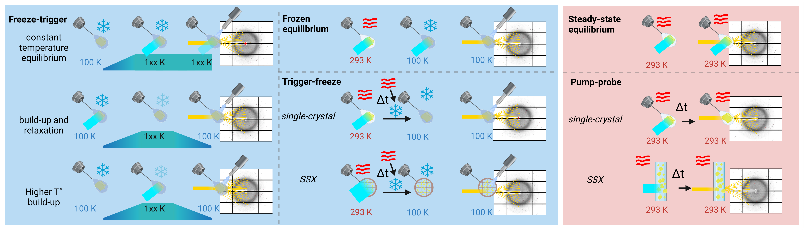
\includegraphics[width=\textwidth]{images/Introduction/Figure1.pdf}
    \hfill
    \caption{Overview of common strategies that can be used to capture the structure of reaction intermediates using light as the reaction trigger. Protocols implicating cryogenic temperature data collection are represented with a blue background: to block a reaction initiated at room temperature once an equilibrium is reached (‘frozen equilibrium’), or before it is reached (‘trigger-freeze’) or to limit the progress of a reaction by initiating it at cryogenic temperature (‘freeze-trigger’). Protocols implicating room-temperature data collection are represented on a red background: to maintain a reaction at equilibrium (‘steady-state equilibrium’) or to catch intermediates as the reaction proceeds (‘pump-probe’). For simplicity, only protocols relying on photoactivation are depicted here. Meaning of symbols: cyan rectangles, UV-visible actinic light; yellow rays, X-rays; red waves, room temperature; blue snowflake, cryogenic temperature}
    \label{fig:Figure1}
\end{figure}

Room-temperature strategies can essentially be divided into two groups. In the first, less used group, the reaction is initiated by illumination until a steady-state equilibrium is reached and data collection is then performed whilst still under illumination (‘steady-state equilibrium’; see, for instance, \cite{crossonPhotoexcitedStructurePlant2002}). In the second group, the experiment is performed under a ‘pump-probe’ sequence. The pump (i.e. laser) pulse is applied at a given time and the probe (i.e. X-ray) pulse is initiated at various delays afterwards. This strategy can be applied to single crystals or to many different microcrystals, to a point where only one still diffraction frame is acquired at most from a microcrystal. Many examples of pump-probe experiments are described in Section \ref{sec:existingfacilities}, Section \ref{sec:BR} and Section \ref{sec:otherlighttrig}. 

\section{Existing facilities and instruments for TR-SFX and TR-SSX}\label{sec:existingfacilities}
TR-SFX experiments have been performed at most existing XFELs. The first experiments were performed at the Linac Coherent Light Source (LCLS), Stanford, California, USA, which opened in 2009. There are essentially two beamlines at the LCLS hosting TR-SFX experiments: CXI (Coherent X-ray Imaging), on which the first experiment was performed with microsecond time resolution on co-crystals of Photosystem I and ferredoxin \parencite{aquilaTimeresolvedProteinNanocrystallography2012}, and MFX (Macromolecular Femtosecond Crystallography), whose first experiment was performed with hundreds of microseconds time resolution on crystals of Photosystem II \parencite{kernStructuresIntermediatesKok2018}. The other pioneering XFEL facility is SACLA in Harima Science Garden City, Hyogo Prefecture, Japan, which opened in 2011, with the first TR-SFX study being performed on beamline BL3 on crystals of bacteriorhodopsin \parencite{nangoThreedimensionalMovieStructural2016}. Beamline BL2 was used for the first time on channelrhodopsin crystals \parencite{odaTimeresolvedSerialFemtosecond2021}. Three other facilities opened later: PAL-XFEL, Pohang, South Korea in 2016, SwissFEL, Villigen, Switzerland in 2017 and EuXFEL, Schenefeld, Germany, also in 2017. The first TR-SFX experiment at SwissFEL took place on beamline ARAMIS-ALVRA using crystals of the light-driven sodium pump KR2 on a wide timescale from hundreds of femtoseconds to tens of milliseconds \parencite{skopintsevFemtosecondtomillisecondStructuralChanges2020}. The first TR-SFX experiment at EuXFEL took place on the SPB/SFX instrument using crystals of PYP at time points in two time ranges: 10-80 ps and 0.89-2.67 ms \parencite{pandeyTimeresolvedSerialFemtosecond2020}. Finally, the new XFEL facilities LCLS-II (at Stanford) and SHINE-XFEL (in Shanghai) will soon be available, as well as beamline ARAMIS-CRISTALLINA at SwissFEL.

Cryo-trapping experiments can be performed on essentially any MX synchrotron beamline, provided that the sample temperature can be precisely controlled. Polychromatic (or Laue) TR-SSX has been performed on the BioCARS beamline at the Advanced Photon Source (APS), Argonne, Illinois, USA to visualize \textBeta-lactam cleavage by a metallo-\textBeta-lactamase using ten snapshots ranging from 20 to 4000 ms \parencite{wilamowskiTimeresolvedVlactamCleavage2022}. Monochromatic TR-SSX experiments have so far been reported on a handful of beamlines. PX1 at the Swiss Light Source (SLS), Villigen, Switzerland was used with a grease injector to track the structure of late intermediates in the photocycle of bacteriorhodopsin \parencite{weinertProtonUptakeMechanism2019}. The TR-SSX capability of I24 at Diamond Light Source (DLS), Didcot, United Kingdom was demonstrated with a study of the photoswitching of the fluorescent protein rsEospa observed 1 ms after light triggering \parencite{baxterObservationCationChromophore2022}. P14.2 (T-REXX) at PETRA III, Hamburg, Germany was the first beamline to be specifically designed for TR-SSX. Its first application was the design of the hit-and-return (HARE) data collection scheme to determine three reaction snapshots for fluoroacetate dehalogenase between 30 ms and 2 s \parencite{schulzHitandreturnSystemEnables2018}. The PETRA III P14 MX beamline has also been used for TR-SSX, with submillisecond time resolution \parencite{kovalevMechanismsInwardTransmembrane2023}. Similarly, steady-state SSX experiments have been performed on the XALOC beamline at ALBA, Barcelona, Spain, also on the sodium pump KR2 \parencite{kovalevMolecularMechanismLightdriven2020}. The build-up of a steady-state equilibrium could be monitored with a time resolution of 63 ms using a serial oscillation crystallography approach on beamline ID30A-3 (MASSIF-3) at the ESRF, Grenoble, France \parencite{aumonierMillisecondTimeresolvedSerial2020}). Finally, dedicated beamlines have recently been designed and constructed at fourth-generation synchrotron sources for TR-SSX: ID29 at the ESRF and MicroMAX at MAX IV, Lund, Sweden.

\section{Potential biases to be considered}\label{sec:potentialbias}
\subsection{Crystal packing}\label{sec:packingartefact}
The first obvious artefact in TR-MX arises from the very fact that the technique requires the molecule to be crystallized, and thus it resides in a significantly different environment than in solution or in the native cellular environment, as molecules are in close interaction with symmetry-related neighbours through crystal contacts and experience a different level of hydration. As a consequence, the crowded but ordered environment in a crystal differs from the dilute environment often used in solution studies and even from the crowded, yet most often unordered, environment of a cell. Protein dynamics components may be either hindered or exacerbated, calling for a verification of whether a reaction proceeds in a similar or a significantly different manner. For instance, it has been shown by both electronic and vibrational transient absorption spectroscopies that the photocycle of PYP differs \textit{in crystallo} from that in solution \parencite{konoldConfinementCrystalLattice2020}. The nature of a few intermediate states differs (the presence of an additional state at an early stage and the absence of an intermediate state at a late stage of the photocycle \textit{in crystallo}), and the rise and decay time constants of equivalent intermediates may vary by more than one order of magnitude. The differences are proposed to be explained by a combination of reduced hydration, different viscosity and confinement in the crystal lattice. In another example, the nature of the intermediate in the photocycle of a LOV (light-oxygen-voltage-sensing) domain is conserved between the solution and the crystalline state, but the kinetics of its decay are significantly affected \parencite{aumonierSlowProteinDynamics2022}. The relaxation decay time constant increases from 6 seconds in solution to 40 s \textit{in crystallo}. This difference is likely to stem from crystal contacts, but may also originate from reduced hydration that could slow down thioether-bond rupture.

\subsection{Temperature}

During the golden age of cryo-crystallography (2000-2010), flash-cooling of crystals at cryogenic temperature was thought to minimally affect the structure of proteins. However, flash-cooling usually requires the addition of cryoprotectant small molecules to the crystal mother liquor, which may specifically bind to the active site of a protein \parencite{bukhdrukerStructuralInsightsEffects2023} and thus affect its function, which can be detected by \textit{in crystallo} optical spectroscopy control experiments in favourable cases \parencite{vonstettenAlterationFluorescentProtein2012}. Moreover, James Fraser and collaborators determined room-temperature crystal structures of proteins and compared them with the cryogenic structures. They found evidence that even though the secondary structure was conserved, a significant proportion of side-chain conformers were altered \parencite{fraserHiddenAlternateStructures2009,fraserAccessingProteinConformational2011}. This means that the conformational landscape of a protein active site can potentially suffer from artefacts stemming from flash-cooling, and the validity of cryo-trapped intermediate states should always be questioned as a matter of principle. Alternatively, freeze-trigger approaches rely on the assumption that the intermediate states populated at low temperatures resemble those of the physiological reaction. This assumption should always be validated by complementary methods, as the conformational landscape may drive the low-temperature photoreaction off the physiological pathway.

\subsection{Radiation damage}\label{sec:raddam}

Radiation damage is an issue inherent to X-ray crystallography \parencite{garmanRadiationDamageMacromolecular2010}. Global damage and specific damage can be distinguished. Global damage affects the diffraction properties of a given crystal (decrease in resolution and increase in mosaicity, unit-cell volume and scaling B factor between successive data sets), which can all be visualized on Bragg peaks (location on the image, shape, intensity; i.e. in reciprocal space). On the other hand, specific damage affects specific chemical groups (carboxylate groups, disulfide bonds, metallic cations), which can all be visualized in electron density maps; \textit{i.e.} in real space) (Fig. \ref{fig:Figure3}). Specific damage was identified by cryogenic data collection at third-generation synchrotrons around the year 2000 \parencite{burmeisterStructuralChangesCryocooled2000,weikSpecificChemicalStructural2000,ravelliFingerprintThatXrays2000}. It was soon realized that the structural changes stemming from specific radiation damage could be mixed up with, or mistaken for, those from intermediate states trapped at cryogenic temperature, and thus hamper precise identification of the latter. This was first observed for bacteriorhodopsin \parencite{matsuiSpecificDamageInduced2002} and later for other systems, some of which contained metallic cations in their active site: horseradish peroxidase \parencite{berglundCatalyticPathwayHorseradish2002}, superoxide reductase in complex with ferricyanide \parencite{adamStructureSuperoxideReductase2004} and a bacterial photosynthetic reaction centre \parencite{baxterSpecificRadiationDamage2004}. In the cases of metal-containing enzymes, the controlled X-ray-induced reduction of the cations is elegantly used to reveal the subtle details of the response of the protein to the change in oxidation state of its metal cofactor that are involved in catalysis. It thus became of utter importance in kinetic crystallography to perform control experiments in order to differentiate structural changes that can be attributed to the build-up of a reaction-intermediate state from those that would develop as a result of specific radiation damage, either of the resting-state structure or on the intermediate-state structure itself.

\begin{figure}[H] %bt!]
    \centering
    \noindent 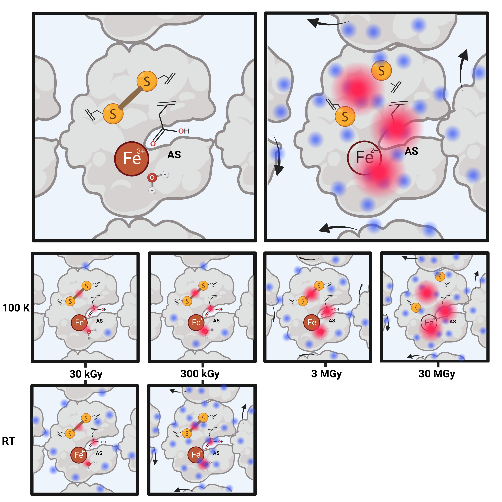
\includegraphics[width=\textwidth]{images/Introduction/Figure3.pdf}
    \hfill
    \caption{Global versus specific radiation damage. Top row, left: a single crystal of a hypothetical protein is depicted with three specific radiation damage-sensitive groups: a disulfide bridge, an oxidized metal cation and a residue with a carboxylate group located in the active site (AS). Top row, right: the crystal is affected by global damage (blue dots) with various effects, in particular that of perturbing crystal contacts upon X-ray-induced protein movement within the cell (black arrows), leading to a loss of diffraction resolution, an increase in mosaicity and increased B factors. Specific damage (red dots) develops on the aforementioned radiosensitive chemical groups, leading to disulfide-bridge reduction (rupture), metal-cation reduction and residue decarboxylation. Middle row: illustration of the damage dose scale at cryogenic temperature. Global damage builds up slowly, while specific damage builds up relatively rapidly, so as to be visible at low doses in Fourier difference maps calculated between successive data sets 1 and n, F\textsubscript{obs}(n) - F\textsubscript{obs}(1), and at high doses in F\textsubscript{calc} - F\textsubscript{obs} and 2F\textsubscript{calc} - F\textsubscript{obs} maps. The maximum acceptable dose is typically that of the Garman limit (30 MGy). Bottom row: illustration of the damage dose scale at room temperature: both types of damage build up on a similar dose scale, complicating the precise identification of specific damage. The maximum acceptable dose for a single crystal is a few hundreds of kilograys, i.e. typically one hundredth of the Garman limit.}
    \label{fig:Figure3}
\end{figure}

The revival of room-temperature crystallography at the end of the 2000s \parencite{fraserHiddenAlternateStructures2009,fraserAccessingProteinConformational2011} prompted the evaluation of how global radiation damage could affect room-temperature structures \parencite{southworth-daviesObservationDecreasedRadiation2007,lealSurveyGlobalRadiation2013} and eventually concluded that full data sets could be recorded in a few hundreds of kilograys from a single crystal. Analysis of these data sets concluded that unlike with cryogenic data sets, specific radiation damage could not be observed clearly \parencite{russiConformationalVariationProteins2017,gotthardSpecificRadiationDamage2019}. It was further suggested that only a small fraction of the molecules in the crystals that contributed to diffraction were affected by this phenomenon \parencite{gotthardSpecificRadiationDamage2019}. This hypothesis was rationalized by showing that specific and global damage occur at similar dose scales at room temperature, but at cryogenic temperature global damage develops much more slowly than its counterpart, constituting a decoupling of these two types of radiation damage. While specific damage is difficult to grasp in single-crystal data sets, the fine dose slicing permitted by SSX led to the clear visualization of specific damage to microcrystals \parencite{schubertMulticrystalDiffractionDatacollection2016,delamoraRadiationDamageDose2020}. One significant bottom line of these observations is that for oscillation MX at a synchrotron, the level of scrutiny required of an intermediate-state structure determined at cryogenic temperature may be relaxed for single-crystal data collection at room temperature, for which specific damage will not be apparent. 

The rapid loss of crystalline order in Photosystem I nanocrystals placed in an intense 100 fs X-ray pulse suggested that specific radiation damage would be an afterthought at XFELs \parencite{bartySelfterminatingDiffractionGates2012}. Yet, it has been shown that long pulses (80 fs) may induce what amounts to specific damage to ironsulfur clusters in ferredoxin by direct photo-ionization of these heavy atoms when compared with 30 fs pulses \parencite{nassIndicationsRadiationDamage2015}. Moreover, pump-probe SFX experiments using two pulses separated by a delay varying between 18 and 112 fs showed the build-up of specific damage to disulfide bonds and the protein backbone in lysozyme and thaumatin \parencite{nassStructuralDynamicsProteins2020}. This has been turned into a trick to study the structural effects of iron(III) photoreduction in the iron-binding protein FutA using a delay time of 33 ms between an attenuated and an unattenuated XFEL pulse \parencite{boltonRedoxSwitchAllows2024}. The effects of microsecond pulses in TR-SSX have only started to be studied, and should soon provide insights into the extent of both global and specific damage in this uncharted time regime.

\subsection{Light fluence}\label{sec:twophoton}

The first TR-SFX studies that were performed did not specifically address the possibility that the fluence of the pump laser illuminating the sample could affect the physiological photoreaction that was probed. As crystals of light-sensitive proteins are highly concentrated in chromophores, the penetration depth of the pump-laser photons is limited to a few micrometres to a few tens of micrometres, depending on the extinction coefficient of the chromophore at the particular wavelength used. Thus, it is tempting to increase the laser power until a meaningful signal can be visualized in a difference electron-density map calculated between a dark and a light data set. The first TR-SFX study to address the potential problem of excessive light fluence used ultrafast visible and infrared spectroscopy to probe the effect of increasing power densities on the photocycle of bacteriorhodopsin \parencite{nasskovacsThreedimensionalViewUltrafast2019}. It was concluded that above a certain threshold the chromophore can sequentially absorb two photons, leading to the excitation of a nearby tryptophan residue. However, no change in the presented structural data obtained with a moderate fluence was ascribed to the artefact identified spectroscopically at higher fluences. Miller and coworkers then proposed that in order to be sure that only a single-photon process is probed in a TR-SFX experiment, the exciting laser power should be kept at a level ensuring an excitation fluence of less than a photon per chromophore within the 1/e absorption depth \parencite{millerThreedimensionalViewUltrafast2020, besawAddressingHighExcitation2023}. The bottom line is that it is of critical importance to evaluate as precisely as possible how many photons are absorbed by crystals in a TR-SFX experiment \parencite{grunbeinIlluminationGuidelinesUltrafast2020}. Also, it is highly advisable to perform power-titration experiments, ideally via both diffraction and spectroscopy \parencite{barendsSerialFemtosecondCrystallography2022}. New instruments have been built to address the same concern for future TR-SSX experiments \parencite{engilbergeTRicOSSetupESRF2024}. One should note that a significant fraction of the incident light is scattered by the sample-carrying medium, which should be estimated and considered in the calculations. Ideally, these power-titration experiments should reveal a linear photoactivation regime, in which additional photons increase the yield of the photoreaction but do not steer it onto artefactual pathways. Performing TR-SX experiments at the maximum laser fluence in the identified linear regime will contribute to optimizing the number of necessary indexed images, thus making the most of the allocated beamtime.

\section{Data processing and analysis}\label{sec:dataprocan} %TODO

\subsection{X-ray diffraction in protein crystals}
When an X-ray beam is shone through a crystal onto an X-ray sensitive surface spots are observed (Fig.\ref{fig:DiffractionPrinciples_1} (a))\footnote{This particular diffraction shot was recorded on BM07-FIP2 (at the ESRF) and comes from the V150A variant of Twist-Cerulean, a fluorescent protein, which will be presented later (Section \ref{sec:V150A})}. These spots mark the location of Bragg peaks: areas of the detector which have received photons which interacted coherently after they were scattered by atoms of the crystal. Solving a structure with X-ray diffraction relies on elastically scattered photons, meaning that their direction is changed by their interaction with the atoms of the crystal, but their wavelength is conserved. A fraction of X-ray photons is always scattered when they go through organic matter, but crystals are a particular form of matter: they are made of a repeated motive: the unit-cell, which is defined by 3 dimension parameters \(a, b, c\) in \AA\ and three angles giving the shape \(\alpha, \beta, \gamma\) in \degree, it contains symmetrically related elements: asymmetric units. The asymmetric unit can be made of one or more monomers for protein crystals. Therefore, there is an orientation of the crystal for which the angle (\(\theta\)) between a set of symmetry atomic planes of the crystal (called \(h,k,l\), and characterised by the distance between them \(d_{h.k.l}\)), and the incident X-ray beam is such that the extra distance travelled by photons (green in Fig. \ref{fig:DiffractionPrinciples_1} (b)) after they are scattered by this plane is a multiple of the wavelength (\textlambda, blue in Fig. \ref{fig:DiffractionPrinciples_1} (b)): they are in phase after scattering (Fig. \ref{fig:DiffractionPrinciples_1} (b)). This condition is called the Bragg law \parencite{drenthPrinciplesProteinXray1999}, and is described by the following equation : 
\begin{equation}\label{eq:bragglaw}
    n\lambda=2d_{h,k,l}sin\theta
\end{equation}
\begin{figure}[H] %bt!]
    \centering
    \noindent 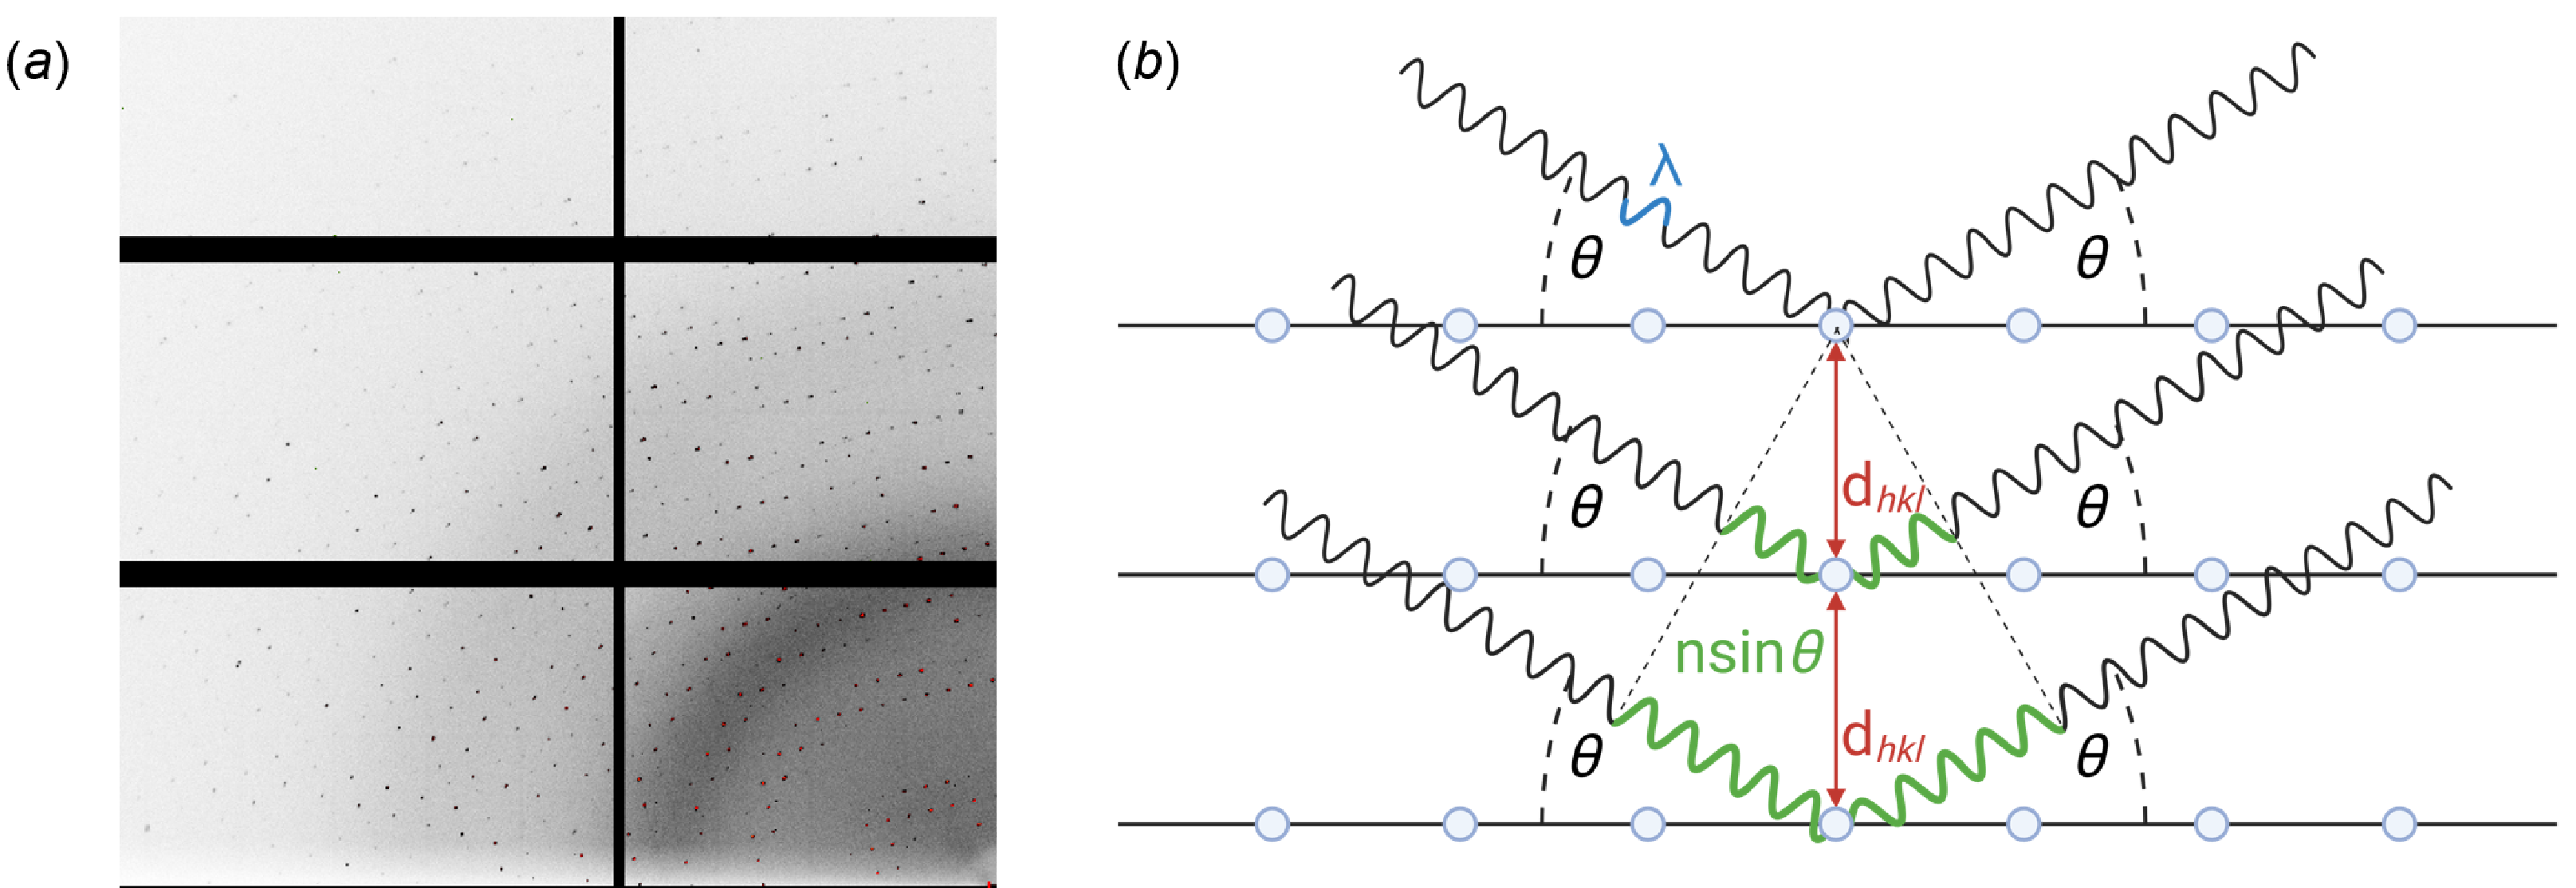
\includegraphics[width=\textwidth]{images/Introduction/Figure_analysis_1.pdf}
    \hfill
    \caption{Principles of X-ray diffraction by protein crystals : (\textit{a}) Diffraction frame  presenting diffraction spots (black to red) as well as an area of diffuse scattering (grey). (\textit{b}) Geometric representation of the Bragg law: coherent interference between diffracted X-ray waves (black sine wave) occurs only when the difference in travel path (green) for photons reflected by adjacent planes is an integer multiple of the wavelength \(\lambda\) (blue). Half the difference in travel path is equal to the distance between the adjacent symmetry planes \(d_{h.k.l}\) (red) multiplied by the sine of the incident angle \(\theta\).} \label{fig:DiffractionPrinciples_1}
\end{figure}
The atoms of the crystals form a lattice (in real space). A Fourier transform of this lattice produces a second lattice, in reciprocal space, in which every node corresponds to crystal planes (identified by their \(h.k.l\) indices) for the conditions of diffractions set by the Bragg law are met. A mathematical construct, the Ewald sphere (represented in Fig. \ref{fig:Ewald}) helps us visualise which reciprocal lattice nodes (represented by hollow dots) can be observed for a specific orientation of the crystal lattice and wavelength of the incoming X-ray beam \parencite{drenthPrinciplesProteinXray1999}: only reciprocal nodes at the surface of the sphere can be observed, and will create a Bragg peak on the detector. The observation of a Bragg peak caused by a reciprocal lattice node crossing the surface of the Ewald sphere and being measured is called a reflection. 

\begin{figure}[H] %bt!]
    \centering
    \noindent 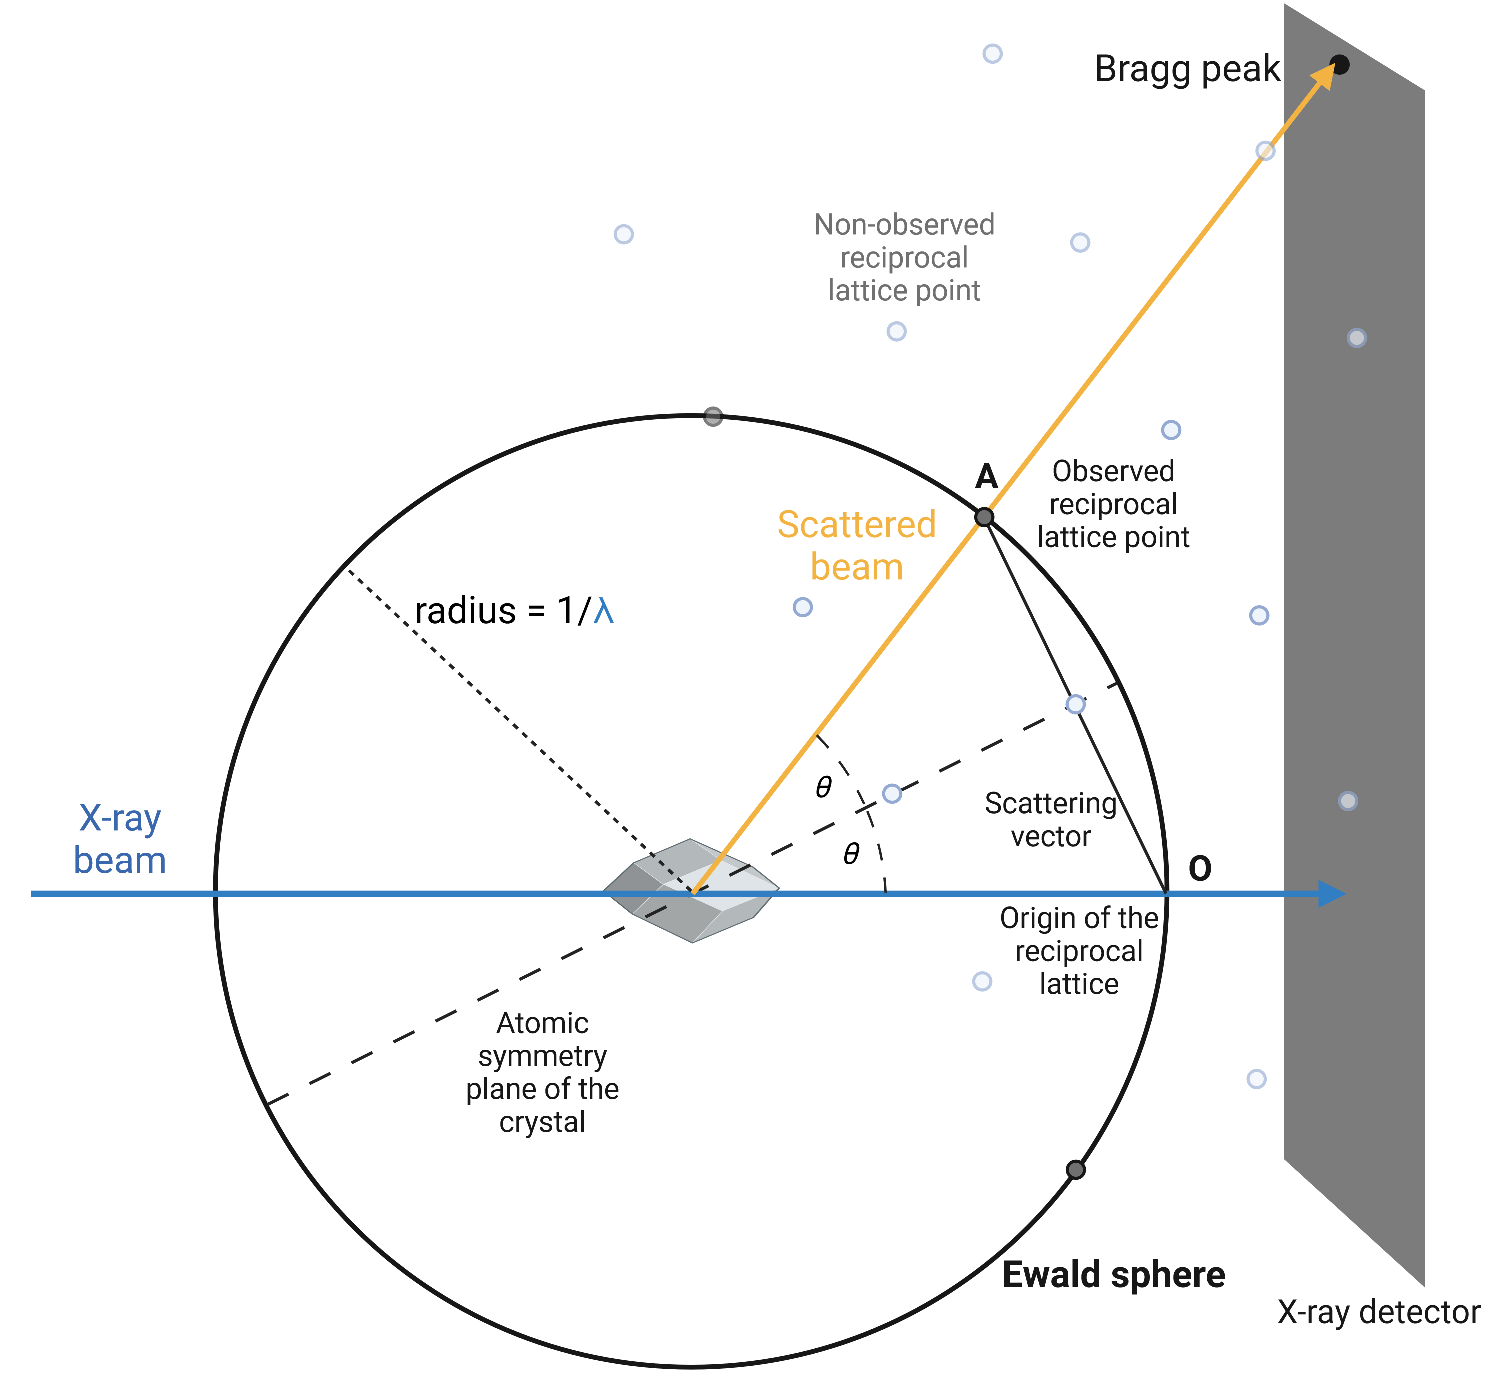
\includegraphics[width=0.8\textwidth]{images/Introduction/Ewald_sphere.pdf}
    \hfill
    \caption{The Ewald Sphere, a representation highlighting in which portion of the reciprocal lattice the conditions for diffraction set by the Bragg law are met (at the surface of the sphere). The orientation of the crystal and its symmetry planes (long dashed lines) determines the orientation of the reciprocal lattice (hollow points) and the direction of the scattered beam (yellow). The wavelength of the incoming beam (blue) determines the radius of the Ewald sphere (short dashed lines). Only reciprocal lattice nodes intersecting the sphere's surface (coloured black and grey) can be observed and will create a diffraction spot on an X-ray-sensitive surface if it is adequately placed. The vector from the origin of the reciprocal space (O) to the exit point of the scattered beam through the Ewald sphere (A) is called the scattering vector, and its length is equal to \(\frac{1}{2d_{hkl}}\)} \label{fig:Ewald}
\end{figure}

The Ewald sphere construction (Fig. \ref{fig:Ewald}) demonstrates that to observe all reciprocal nodes, crystallographers must measure over a range of \(\theta\) (crystal orientations) or \textlambda. The first TR-MX Laue (polychromatic) experiments described in Section \ref{sec:history} used a wide range of \textlambda\ to increase the total photon flux, which increases the thickness of the Ewald sphere and allows the simultaneous measurement of more reflections (Fig. \ref{fig:Ewald}). However, most MX experiments use a monochromatic X-ray beam (fixed \textlambda) and continuous variation of the crystal orientation (\(\theta\)). %The intensity of the Bragg peak measured on the detector is a function of the density of the electron (that is to say, the number and type of scattering atoms) and the scattering angle (\(\theta\)), among other things. 

In practice, because the surface of the Ewald sphere is thin (monochromatic beam with narrow bandwidth), a reciprocal lattice node is intersected, but not fully covered by the surface of the Ewald sphere (Fig. \ref{fig:Ewald}). Historically, to make sure that diffraction frames contained the scattering contribution of an entire reciprocal lattice node, crystallographers rotated or oscillated the crystal in the beam during the measurement \footnote{All data recorded this way will be referred to as rotation data or standard MX}. With this method, the reciprocal lattice is rotated into the surface of the sphere, and the covered area is two moon crescents (lunes).

\subsection{Data processing for classical crystallography}\label{sec:classic}

Any protein diffraction experiment then aims at \textbf{(1)} finding Bragg peak coordinates on the detector (referred to as spot-finding), \textbf{(2)} identifying the reciprocal lattice node they originate from (referred to as indexing), \textbf{3} integrating the Bragg peak (measuring the intensity of the scattered beam). In practice, each reciprocal lattice node is measured many times, at different scattering angles, which adds another step to the process: \textbf{4} scaling and merging different observations. Steps 1-3 were performed with XDS \parencite{kabschXDS2010}, and step 3 with AIMLESS \parencite{evansHowGoodAre2013} for all rotation data collected during this thesis. The electron density at a given point of the unit cell can be accessed through a Fourier transform of the structure factors (representing all scattering contributions from the unit cell, and obtained from the intensities by using the TRUNCATE program of the CCP4 suite \parencite{agirreCCP4SuiteIntegrative2023}). Importantly, only the intensity of a reflection (how much X-ray was scattered) is measured in MX, not the phase of the scattered X-ray beam. Nowadays, phases are almost exclusively extracted from the molecular model of another structure or \textit{in sillico} model obtained with AlphaFold \parencite{jumperHighlyAccurateProtein2021, abramsonAccurateStructurePrediction2024} or RoseTTAFold \parencite{baekAccuratePredictionProtein2021}, via molecular replacement. 

\paragraph{Spot-finding:} The first step in crystallographic data processing is to identify Bragg peaks, contiguous regions where pixels of the detectors have a reading higher than the background level \parencite{drenthTheoryXrayDiffraction1999}. This is achieved by calculating the average background level on specific concentric slices of the X-ray detector centred on the beam's position, because of the presence of diffuse X-ray scattering produced by non-crystalline elements in the sample, visible in Fig. \ref{fig:DiffractionPrinciples_1} (a).

\paragraph{Indexing} Because the detector-sample distance and X-ray wavelength are known, the coordinates of the Bragg peaks can be converted to scattering vectors. The distance between consecutive Bragg peaks in a pattern (Fig. \ref{fig:DiffractionPrinciples_1} (a)) is determined by the distance between reciprocal lattice nodes (related to the distance between the crystal lattice points). This gives access to the unit-cell parameters \parencite{kabschAutomaticIndexingRotation1988}. Then, each scattering vector (Fig. \ref{fig:Ewald}) is assigned to a crystal plane, and given \(h,k,l\) indices and the probability of each possible space group is estimated, eventually using prior knowledge from the orientation of adjacent frames.  

\paragraph{Integration} A reflection 'mask' identifying the position of all potential Bragg peaks is created from the knowledge of the crystal lattice parameters, symmetry and orientation. The background in each position is estimated taking into account scattering such as the ring visible in Fig. \ref{fig:DiffractionPrinciples_1} (a). Finally, a profile shape is determined by two parameters fitted on the strongest Bragg peaks of the frame, and fitted to each reflection taking into account the divergence of the beam, and position in the lune of the Ewald sphere \parencite{kabschXDS2010}. 

\paragraph{Scaling and merging} Experimental factors such as the length of its scattering vector, X-ray absorption by the crystal, variation of the photon flux and volume of crystal traversed by the beam during the measurement all contribute to the measured intensity of a reflection \parencite{evansHowGoodAre2013}. The onset of global radiation damage (see Section \ref{sec:raddam}) and the contribution of thermal motion (characterized by Debye-Waller factors), may lead to a gradual decrease in intensity over time. Related measurements help create a scaling profile over the detector range, and the data-collection. To ensure data quality, most crystallographers record more than the minimal angular range needed to fully sample the reciprocal space. Thus, after scaling, all measurements of the same reflection are merged to ensure a robust estimate of the intensity \footnote{According to Friedel's law, the intensity of a diffracted X-ray beam in the direction of a reciprocal lattice node \(h\) is equal to the intensity in the opposite direction \(-h\). If the experimenter is not interested in anomalous scattering, measurements arising from the diffraction in the direction \(h\) and \(-h\) can also be merged.}. 

\subsection{Merging data from several crystals}

The first attempts at protein and macromolecule crystallography required merging the data from several crystals because a single crystal would not survive its exposure to the X-ray source at ambient temperature for long enough to allow the collection of a full diffraction dataset \parencite{kendrewThreeDimensionalModelMyoglobin1958, perutzStructureHaemoglobinThreeDimensional1960, blakeStructureHenEggWhite1965}. While cryocrystallography elegantly overcame that initial issue \parencite{hopeCryocrystallographyRibosomalParticles1989}, merging data from several crystals remained a strategy to study particularly X-ray sensitive species \parencite{fedorovCrystalStructuresMolecular2003} or targets which would only crystallise in crystals too small to withstand the collection of a full dataset, even at cryogenic temperature. The main hurdle to overcome in this situation is the potential lack of isomorphism between collected datasets. Indeed, while crystallographers generally operate under the assumption that merging more data will increase the quality of the resulting datasets, that is true only when the datasets are similar enough. Such experimental strategies will be referred to as 'multi-crystal approaches'. Several strategies were developed to select the best combination of wedges from different crystals. A multi-crystal-based TR-MX approach has been developed and will be covered in Section \ref{sec:LOV2_TR-SOX}.

\subsubsection{Hierarchical Clustering Analysis} 

Hierarchical clustering analysis (HCA) groups datasets which are coherent with each other. HCA relies on the calculation of pairwise distances, based on particular metrics. A dendrogram is then constructed between each element of the set, based on that distance. Each node of this dendrogram represents a subset of wedges, and the user can survey the statistics for each subset and choose their preferred tradeoff between completeness and data homogeneity, usually measured by the \(CC_{1/2}\) \parencite{karplusLinkingCrystallographicModel2012} of the dataset. 

The most straightforward distance metric is the difference in lattice parameters, implemented in BLEND \parencite{foadiClusteringProceduresOptimal2013} \footnote{This approach was originally developed to solve the structure of a G-protein coupled receptor, which only produced small crystals \parencite{hansonCrystalStructureLipid2012}. Radiation damage, at cryogenic temperatures, increases the volume of the unit-cell \parencite{naveUnderstandingRadiationDamage2005}, Hanson and colleagues selected the populations of lattice parameters least radiation damaged. Experiments realised on non-radiation damage-sensitive samples still benefit from this approach, because crystals of different sizes might cryo-cool at different rates, and crystals maintained at room temperature might not have identical humidity levels, leading to changes in lattice parameters which can decrease the quality of the final merged dataset. However, the estimation of lattice parameters is often poor for wedges containing few images.}. The correlation coefficient of intensities in shared reflection between datasets also quantifies structural differences and is an overall more robust distance metric \parencite{giordanoApplicationHierarchicalCluster2012, zanderMeshAndCollectAutomatedMulticrystal2015, santoniHierarchicalClusteringMultiplecrystal2017, yamashitaKAMOAutomatedData2018}. 

\subsubsection{Genetic Algorithms} 

Genetic Algorithms (GA) are evolution-inspired. Wedges are originally randomly dispersed in a series of wedge sets, called a generation. First, the most 'fit' sets are selected. The fitness score proposed in \cite{zanderMergingSynchrotronSerial2016} relies on merging statistics. Then, pairwise crossovers (exchanges of wedges between sets) and mutations (substitutions of one wedge for another in a set) are performed. These steps are repeated until the algorithm converges into a set that maximises fitness. While considerably more computationally intensive than the HCA, the GA select datasets based on their merging statistics, not inner coherence. 

\subsection{Serial Crystallography}\label{sec:SX_intro}

Depending on the authors, the term 'serial crystallography' (SX) also encompasses multi-crystal approaches. In this thesis, SX refers only to the experiments where each crystal is briefly exposed to the X-ray beam only once, without rotation (described in Section \ref{sec:history}. In these experiments, all reflections measured on the detector are partially integrated (still images) \footnote{Albeit there are instances where the reflections are integrated over the wavelength of the incident beam, for pink beam crystallography \parencite{meentsPinkbeamSerialCrystallography2017} or the slightly larger bandpass of ID29 \parencite{griecoStructuralDynamicsFunctional2024}.}. 

\subsubsection{Processing serial crystallography data}

During this thesis, all SX data was processed within the CrystFEL environment \parencite{whiteCrystFELSoftwareSuite2012} which workflow is presented in Fig \ref{fig:CrystFEL}In SX, a medium carrying micro-crystals is shot by an X-ray beam (sometimes pulsed) with high frequency thereby generating a high number of images of which an important fraction does not contain diffraction. The first step of SX processing is therefore to identify images containing diffraction (hit-finding), discard all empty frames, and find the position of the Bragg peaks in hit frames (peak-finding). This is often performed on the fly, to avoid storing unnecessary images. The hit rate (\% of images containing diffraction) is monitored as a performance metric for the sample delivery system. 

Indexing still images is challenging, as the Bragg peaks measured are often smaller and weaker than those of rotation MX images. \textit{indexamajig}, the indexing tool of CrystFEL, allows the use of several indexing algorithms, one after the other, so that if the first fails, a second can be tried, and so on. We have used algorithms xGandalf \parencite{gevorkovXGANDALFExtendedGradient2019}, MOSFLM \parencite{powellRossmannFourierAutoindexing1999} and TakeTwo \parencite{ginnTakeTwoIndexingAlgorithm2016} to index, in that order. Once an indexing solution is found, CrystFEL integrates areas of potential Bragg peaks - often many more than the Bragg peaks picked up by the peak-finder - by profile fitting. The indexing rate and histograms of lattice parameters (ideally monodisperse with sharp peaks, whose parameters are coherent with the indexing solution) serve as a proxy for the quality of data collected. The indexing solution, Bragg peaks intensities and position are all stored in a text-formatted file, the stream-file. 

SX data processing requires a geometry file, describing the sample environment and detector which are often more complex than in rotation MX: they rely on multiple panel detectors and sample environment where the detector-sample distance can be unstable. Most frequently, the stream file containing the indexing solutions and reflection intensities is fed into Geoptimiser \footnote{In the last versions of CrystFEL, Geoptimiser was replaced with a much more efficient algorithm called the 'millipede approach' which has not been published by Tom White yet. }, an algorithm refining the various geometry parameters (panel positions, orientation, beam position), and a range of detector-distance values are sampled to maximise data quality and consistency. This step is often performed from a starting geometry provided by the beamline staff and using a well-known crystalline sample whose lattice parameters are stable, such as lysozyme. This is, however, becoming a lesser issue as beamlines with stable setups and fixed geometry (T-REXX at PETRA III, ID29 at the ESRF, Cristallina at SwissFEL) emerge.

In SX, each measured intensity represents a fraction of the intensity of its full reflection, exactly which fraction must be determined (partiality estimation): many partial measurements of the same intensity are merged into a full intensity: the partiality of each measurement is refined against the other measurements of the same intensity, and the other measurements present on that diffraction frame. Then, all intensities are scaled with parameters described in Section \ref{sec:classic}. The merging algorithm of CrystFEL, \textit{partialator}, performs these three steps simultaneously by iteratively refining the partiality and scaling terms of each measurement before merging. \textit{partialator} produces data quality indicators (\(CC_{1/2}\) and \(CC^\ast\) described in \cite{karplusLinkingCrystallographicModel2012,karplusAssessingMaximizingData2015}, signal/noise ratio) which are used to set to manually refine the resolution cutoff and merge again. CrystFEL outputs intensities, which are eventually converted to structure factors. 

\begin{figure}[H] %bt!]
    \centering
    \noindent 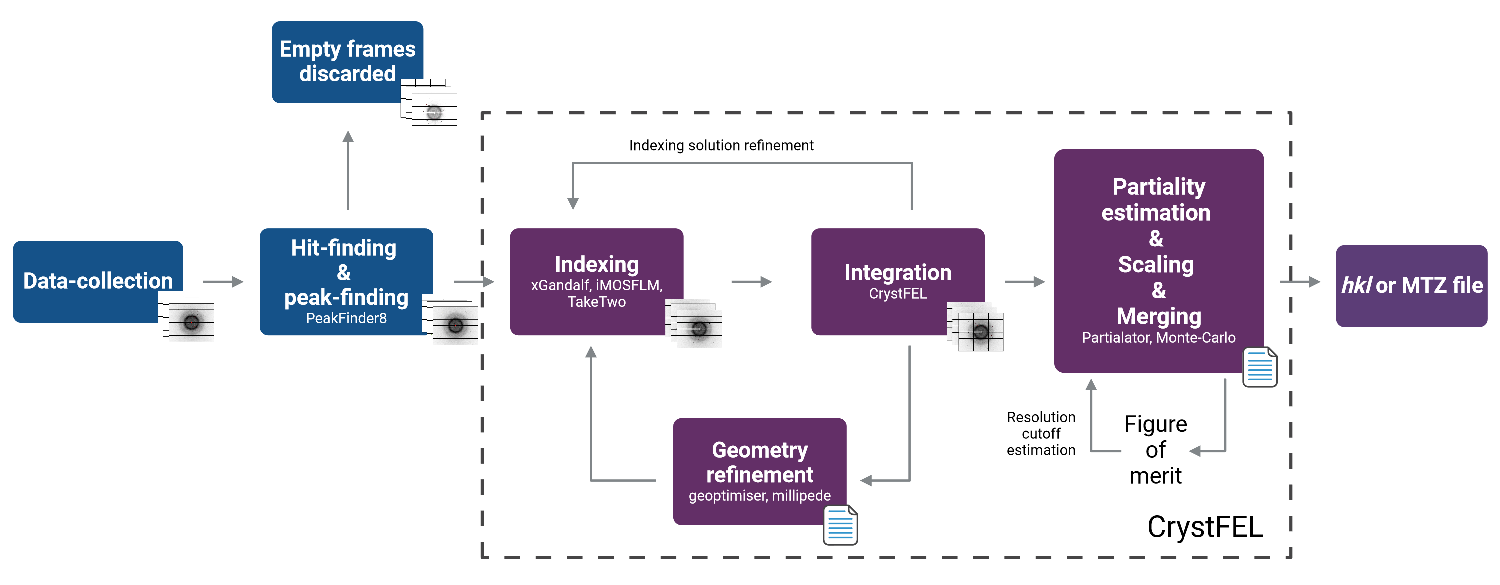
\includegraphics[width=\textwidth]{images/Introduction/SX_data-processing.pdf}
    \hfill
    \caption{SX data processing within the CrystFEL environment, step by step} \label{fig:CrystFEL}
\end{figure}

\subsection{TR-MX data analysis}

In theory, model building and refinement for all TR-MX data could be carried out right after merging, with the tools used for rotation crystallography. In practice, the contribution to diffraction in TR-MX experiments arises from a mix of resting state protein and one or more reaction intermediate states. Disentangling this mix is challenging as it involves determining both the occupancy (share of the molecules in the crystal in a current state) and the nature of these unknown reaction intermediate states.

\subsubsection{Isomorphous difference maps and how to analyse them}

The gold standard for the analysis of TR-MX data is the isomorphous \(F_{obs}(time\ point)- F_{obs}(ground\ state)\) electron density difference map \parencite{rouldIsomorphousDifferenceMethods2003}, for which the structure factors from the two datasets are scaled, and an electron density map is calculated from the structure factors resulting of their difference. Ideally, this map is mostly flat and contains local positive and negative electron density peaks highlighting the most prominent differences in the structures. This method relies on the assumption that the two datasets are mostly similar and, importantly, that their lattice parameters are similar. If the crystal lattices of both crystals are not isomorphous, the calculated map becomes meaningless as the two reciprocal lattices are sampling real-space differently. When dealing with datasets with lower signal/noise ratio, Bayesian scaling can enhance the signal in the isomorphous \(F_{obs}(time\ point)- F_{obs}(ground\ state)\) electron density difference map \parencite{ursbyImprovedEstimationStructureFactor1997}. The scaling terms and R\textsubscript{factors} produced during the scaling phase (ideally constant over resolution and <0.25) can be used as proxies for the compatibility of the two lattices. Tools to calculate real-space difference maps exist but only correct the difference in lattice parameters and won't produce a meaningful difference if the two structures are overall too different \parencite{brooknerMatchMapsNonisomorphousDifference2024}.

The most straightforward way to identify trends in a series of isomorphous \(F_{obs}(time\ point) - F_{obs}(dark)\) maps is to integrate the electron density over time in a region of interest \cite{wickstrandToolVisualizingProtein2020}. This way, specific features of the maps can be assigned time-stamps, and an overall sequence of events can be derived. A more complex solution is the deconvolution of the map series (in real space) via Singular Value Decomposition (SVD), an algebra-based (eigenvalue decomposition of a matrix) analysis technique which has been widely used in time-resolved spectroscopy \parencite{henrySingularValueDecomposition1992,henryUseMatrixMethods1997} and more recently in TR-MX \parencite{schmidtApplicationSingularValue2003}. SVD produces structural components (in the form of a real-space electron density map) and their time-dependent combination (in the form of a series of scalar indicating the strength and polarity of each component over time). SVD analysis can effectively set apart meaningful trends from noise-induced features in the series. Of note, a variation of SVD called non-negative matrix factorisation can be used to analyse standard electron density maps \parencite{christouTimeresolvedCrystallographyCaptures2023a}. During this PhD, we developed a set of tools to perform SVD analysis (Sections  \ref{sec:SVD_Methods}; \ref{sec:SVD_MmCPDII} and \ref{sec:TR-SOX_SVD}) and check the validity of the interpretation it produced (Section \ref{sec:SVD_CraCRY}). SVD and integration produce a sequence of events, based on which the models of reaction intermediate states can be built.

\subsubsection{Model building for TR-MX}

Model-building in MX consists of the iterative refinement of a set of atomic positions, but also of temperature factors, scaling factors and bulk solvent corrections, with restraints from chemical properties of the molecules in the crystal, to minimise the difference between the measured structure factors (\(F_{obs}\)), and the structure factors calculated from the model (\(F_{calc}\)). During this PhD, this step, performed with REFMAC5 \parencite{murshudovRefinementMacromolecularStructures1997, yamashitaGEMMIServalcatRestrain2023} was alternated with visual inspection and real-space refinement in COOT \parencite{emsleyFeaturesDevelopmentCoot2010}. At its core, refinement relies on R\textsubscript{work} and R\textsubscript{free}. R\textsubscript{work} quantifies the difference between \(F_{obs}\) and \(F_{calc}\): the agreement of the model with the data. R\textsubscript{free} quantifies the difference between \(F_{calc}\) and a small subset of \(F_{obs}\) (5 \%), which has not been used to refine the model. The difference between Rwork and Rfree helps detect model overfitting. Typically, MX models only contain one conformation for each amino acid and occasionally alternate conformations of specific amino acids. For these few cases, the occupancy (\% of conformation A and conformation B) is refined. In TR-MX, the model should contain several distinct copies of a great number of amino acids, corresponding to each of the reaction species existing in the crystal at the time of data collection. Each of these copies has its own set of parameters, and attempting to refine such a model would quickly lead to overfitting (revealed by a drop in R\textsubscript{work} and an increase in R\textsubscript{free}). 

The simplest approach to refine a model for TR-MX datasets is to fix all parameters for one of the copies of the protein (or entire regions of the structures) and only refine a smaller alternate model for each state, one at a time (\cite{nangoThreedimensionalMovieStructural2016}, Section \ref{sec:BR}). This method was developed to refine datasets collected with a pump-probe scheme, in which \textasciitilde two species exist at any time: a majority of the ground state (fixed) and a minority of reaction intermediate state (refined). This is how the models discussed in Chapter \ref{chap:slowprot} were refined. Alternatively, atomic positions can be varied over a trajectory to maximise the correlation between the isomorphous \(F_{obs}(time\ point) - F_{obs}(dark)\) map and a calculated \(F_{calc}(time\ point) - F_{calc}(dark)\) map (\cite{maestre-reynaSerialCrystallographyCaptures2022, maestre-reynaVisualizingDNARepair2023a}, Section \ref{sec:photoenzymes}. This approach does not require chemical restraints which is beneficial for the refinement of high-energy reaction intermediates, whose geometries strongly differ from crystallographic libraries. Finally, the crystallographic data can be used to guide MD simulations starting from a static-state model \parencite{grosInclusionThermalMotion1990,pearceMethodIntuitivelyExtracting2021}, which are then used in refinement with translation-libration-screw (TLS) modelling large segments of the protein with limited parameter weight \parencite{schroderSuperresolutionBiomolecularCrystallography2010,schroderDeformableElasticNetwork2014}.

Orthogonal to multi-copy refinement, extrapolation aims at extracting a set of structure factors corresponding to a reaction intermediate state at full occupancy, \(F_{extrapolated}\) from a dataset \(F_{obs}(time\ point)\) by subtracting the ground state structure factors \(F_{obs}(ground)\) using a Bayesian scaling term, \(w\) (equation \ref{eq:extrapolation}, \cite{genickStructureProteinPhotocycle1997}, \cite{dezitterXtrapol8EnablesAutomatic2022}). 
\begin{equation}\label{eq:extrapolation}
    F_{extrapolated} = w \times \alpha \times (F_{obs}(time\ point) - F_{obs}(ground)) + F_{obs}(ground)
\end{equation}
In equation \ref{eq:extrapolation}, \textalpha\ quantifies the occupancy. For all the methods described above, decreasing the occupancy of the reaction intermediate will cause the model to adopt conformations further different from the ground state (this is particularly true for extrapolation) \parencite{vallejosAppraisingProteinConformational2024}. Determining the occupancy of an intermediate state is pivotal in TR-MX model building. During this PhD, we developed several methods to solve this challenge, based on crystallographic data analysis (Section \ref{sec:LOV2_slow_occupancy}) or using \textit{in crystallo} optical spectroscopy as an orthogonal method to assess the occupancy of a state (Chapter \ref{chap:slowprot}, \ref{chap:online-microspec}, \ref{chap:TR-icOS} and Section \ref{sec:CraCRY_TR-icOS}).


\section{Bacteriorhodopsin: an emblematic example of fast TR-MX}\label{sec:BR}

Bacteriorhodopsin (BR) is a light-driven proton pump that is found in the membrane of the halophilic archaeon \textit{Halobacterium salinarum} \parencite{oesterheltRhodopsinlikeProteinPurple1971}, which has served as a paradigm for both the spectroscopic and structural characterization of membrane proteins \parencite{ottolenghiPhotophysicsPhotochemistryRetinal1995,hauptsCLOSINGBACTERIORHODOPSINProgress1999}. BR is composed of seven transmembrane helices, and its chromophore retinal is covalently bound through a Schiff-base linkage to a lysine residue (Lys216) located in the middle of the seventh helix (helix G). Upon the absorption of a photon by its retinal chromophore, the protein adopts a succession of spectroscopic states characterized by specific UV-Vis absorption maxima before returning to the ground state, forming a photocycle (Fig. \ref{fig:Figure4} \textit{a}). The successful crystallization of bacteriorhodopsin in lipidic cubic phases \parencite{landauLipidicCubicPhases1996} led to the determination of its crystal structure at increasing resolutions \parencite{pebay-peyroulaXrayStructureBacteriorhodopsin1997, beitlichCryoradiolyticReductionCrystalline2007}, paving the way for high-resolution structures of intermediate states in its photocycle. Because of the significant mosaicity of the crystals, the room-temperature approach using Laue diffraction never materialized, and the first period of structural characterization of the BR photocycle relied entirely on cryo-trapping \parencite{wickstrandBacteriorhodopsinWouldReal2015}.
\begin{figure}[H] %bt!]
    \centering
    \noindent 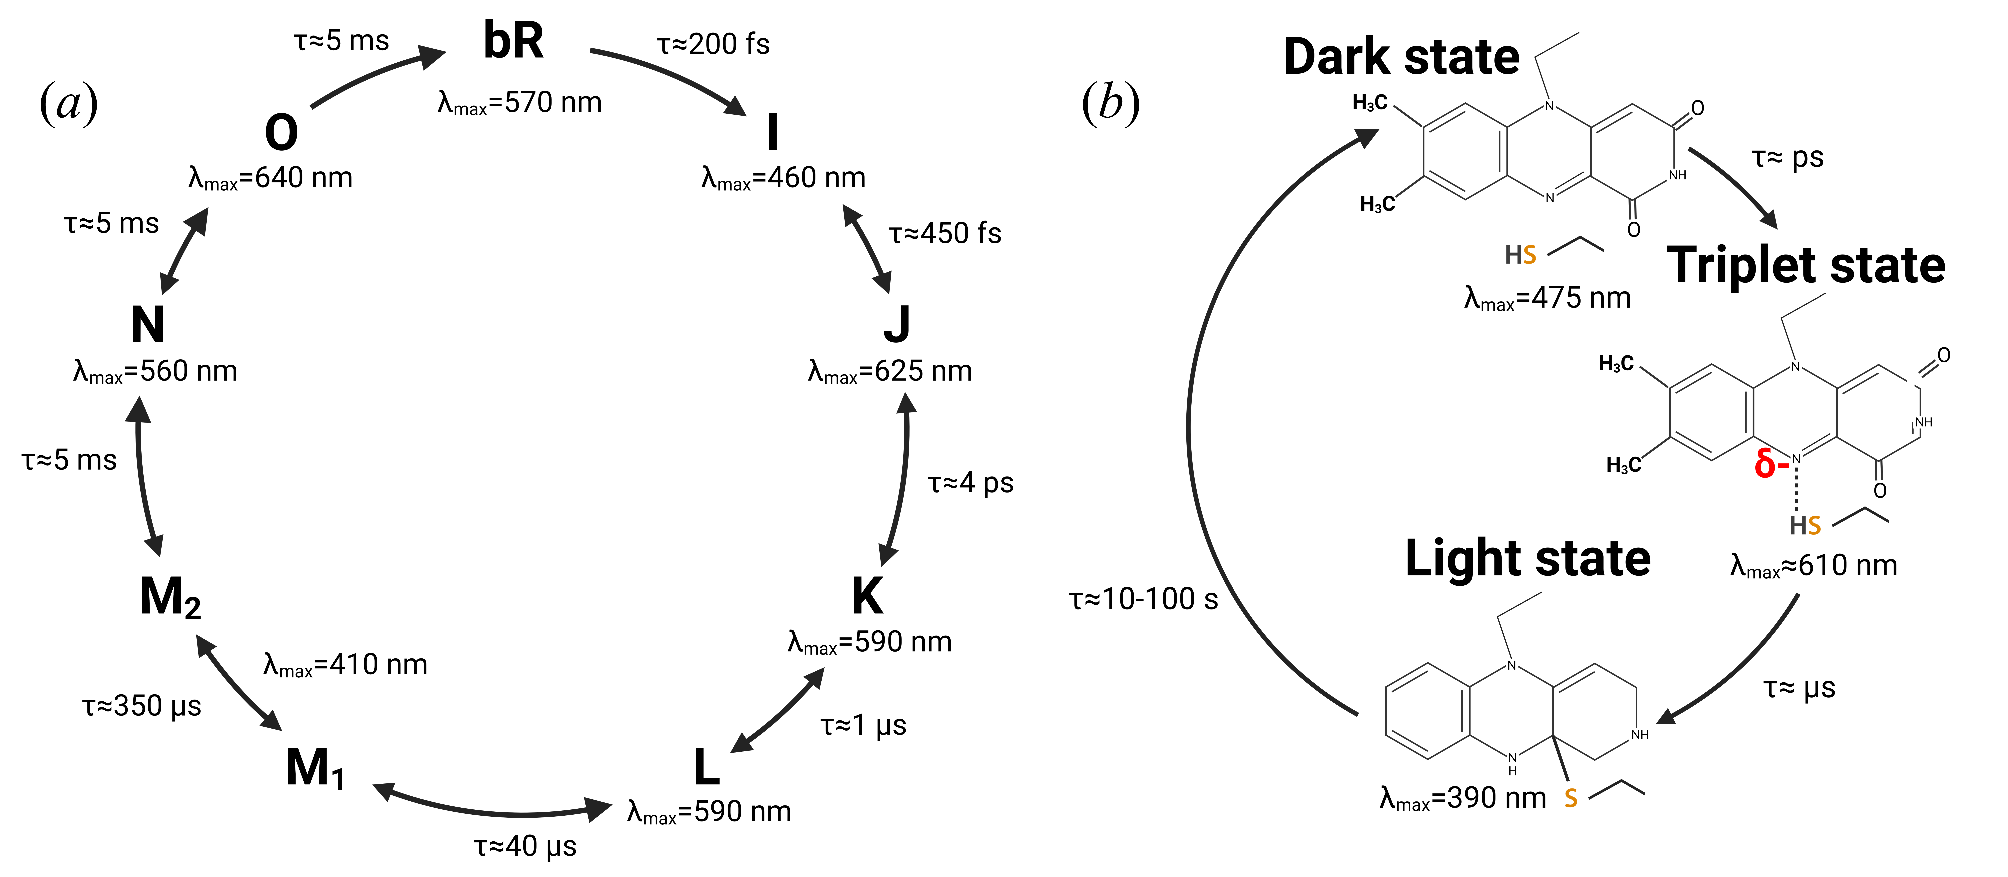
\includegraphics[width=\textwidth]{images/Introduction/Figure4_photocycles.pdf}
    \hfill
    \caption{Photocycles of (a) bacteriorhodopsin and (b) a LOV domain. }
    \label{fig:Figure4}
\end{figure}

\subsection{Cryotrapping studies}

The first crystallographic study of a BR photoreaction intermediate was that of the K state populated at low temperature (110 K) upon illumination with green light \parencite{edmanHighresolutionXrayStructure1999}. The structural changes are confined to the environment close to the chromophore, with signs of retinal isomerisation, disordering of a water molecule that was previously in a hydrogen-bond interaction with the Schiff-base nitrogen, and movement of neighbouring residues. A later study on the L state \parencite{royantHelixDeformationCoupled2000}, which was populated at a higher cryogenic temperature (170 K), revealed that the perturbation of the hydrogen-bond network had progressed towards the extracellular side of the protein. At the same time as this study, a structure of the M state was obtained \parencite{sassStructuralAlterationsProton2000}. These three studies performed on the wild-type protein provided an initial structural picture of the events following light absorption by the chromophore retinal and leading to its deprotonation \parencite{kuhlbrandtBacteriorhodopsinMovie2000}. A number of studies on BR mutants and also on wild-type BR with different trapping protocols followed, yielding conflicting results, thus providing a blurred picture of what could really be precisely achieved by cryo-trapping methods \parencite{wickstrandBacteriorhodopsinWouldReal2015}. Another complicating factor was the realization that specific radiation damage affected the structure of the ground and K states of BR at low dose \parencite{matsuiSpecificDamageInduced2002, borshchevskiyXrayRadiationInducedChangesBacteriorhodopsin2011, borshchevskiyLowdoseXrayRadiation2014}. A recent effort towards maximizing diffraction resolution provided an improved picture of the K, L and M states, most particularly regarding the presence of hydrogen bonds \parencite{borshchevskiyTrueatomicresolutionInsightsStructure2022}. Nonetheless, the controversies regarding the structure of cryotrapped intermediates in the BR photocycle set the stage for time-resolved studies at room temperature.

\subsection{XFEL studies}

After a feasibility study on the M state \parencite{noglyLipidicCubicPhase2016}, the first breakthrough XFEL study used a nanosecond pump laser and aimed to probe the structural events ranging from the K state, which builds up in picoseconds and is thus well present at nanoseconds, to the onset of the large structural changes occurring to helices that are expected in the M2 state after a build-up over several hundreds of microseconds \parencite{nangoThreedimensionalMovieStructural2016}. At 16 ns, isomerisation of the retinal is completed, displacing a tryptophan residue on helix F and initializing the perturbation of the hydrogen-bond network bridging the chromophore and the extracellular side. The perturbation progressively develops to prepare the irreversible proton transfer from the retinal Schiff-base nitrogen to the primary acceptor (Asp85) through the transient ordering of a water molecule and the concomitant release of a proton into the extracellular medium. Conversely, structural changes in the cytoplasmic part develop in the microsecond to millisecond regime, setting up the conditions for retinal reprotonation from the cytoplasm. However, the latest time point at 1.7 ms did not reveal large changes of the cytoplasmic part, calling into question whether the crystal form would not completely hinder them. 

\begin{figure}[H] %bt!]
    \centering
    \noindent 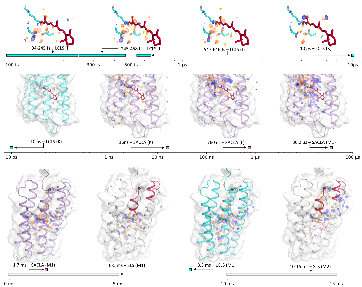
\includegraphics[width=\textwidth]{images/Introduction/Figure5_Bacteriorhodopsin.pdf}
    \hfill
    \caption{Overview of structural changes in the photocycle of BR visualized by TR-SFX and TR-SSX over 13 orders of magnitude. Fourier difference maps (yellow, negative; blue, positive) are contoured at the 3.9 RMSD level in the top row and at the 3.0 RMSD level in the middle and bottom rows, and are superimposed on the corresponding ground-state structure. Data are reprised from a TR-SFX study performed at SACLA (lilac; \cite{nangoThreedimensionalMovieStructural2016}, a TR-SFX study performed at the LCLS (cyan; \cite{noglyRetinalIsomerizationBacteriorhodopsin2018} and a TR-SSX study performed at the SLS (white; \cite{weinertProtonUptakeMechanism2019}. The parts of helices E, F and G depicted in red in the SLS structures are those that undergo large-scale displacement or disordering in the late phase of the photocycle.}
    \label{fig:Figure5}
\end{figure}

The second XFEL effort aimed to understand the very first steps in the photocycle of bacteriorhodopsin using a femtosecond laser instead \parencite{noglyRetinalIsomerizationBacteriorhodopsin2018}. This led to the visualization of the response of the protein and chromophore to the absorption of a green photon from hundreds of femtoseconds to 10 ps, covering the build-up and decay of the first three intermediates I, J and K, with the addition of an 8.33 ms time point acting as a reference for the M state, which is very consistent with the 1.7 ms time point recorded in the previous experiment (Fig. \ref{fig:Figure5}). The various snapshots are consistent with a mechanism in which the electronically excited chromophore initially samples possible isomerisation geometries (as suggested by the number of negative peaks along the retinal chain at t < 458 ps), before C13 C14 is selected (J state; 457-636 fs, rotated bond), until a twisted isomerized chromophore builds up in the K state at 10 ps. The collective motions of the primary acceptor Asp85, the neighbouring Asp212 and close water molecules during this process are proposed to illustrate how these chemical groups favour the stereoselectivity and efficiency of retinal isomerisation. A parallel study proposed a very similar view of the first steps of the response of retinal to light absorption in bacteriorhodopsin \parencite{nasskovacsThreedimensionalViewUltrafast2019}. A useful lesson from this study is the spectroscopic evidence that multiphoton absorption may occur in TR-SFX experiments, calling for a better control of light fluence see section (Section \ref{sec:twophoton}).

\subsection{Synchrotron studies}

BR has often been used as a target in the development of SX experiments at synchrotrons (SSX experiments; \cite{noglyLipidicCubicPhase2015, zanderMeshAndCollectAutomatedMulticrystal2015}. Appropriately, it became one of the first systems to successfully be used in TR-SSX experiments. Building on the TR-SFX results, Weinert and coworkers designed an experimental setup on beamline PX1 of the SLS that was able to track structural changes in the BR photocycle by illuminating a moving grease jet of crystals for 5 ms with a CW class 3R green laser diode (520 nm; \cite{weinertProtonUptakeMechanism2019} every 200 ms. The EIGER detector was operated at 200 Hz, so that the first frame of a cycle corresponded to crystals under illumination (the 0-5 ms frame), while the 39 later frames corresponded to increasing delays in a pump-probe scheme from 5-10 ms to 195-200 ms. While the diffraction data were at moderate resolution, the 5-10 ms time point fittingly showed structural features associated with the M state visualized in previous studies (Fig. \ref{fig:Figure5}). However, the following time point, 10-15 ms, revealed the build-up of an open form of the protein, with large-scale movements or disordering of the cytoplasmic parts of helices E-G, with the largest displacement (9 \AA) occurring at the tip of helix F. These changes must be associated with the N state only, as the O state has been shown to hardly be populated in crystals of BR \parencite{efremovPhysicalDetwinningHemihedrally2004}.

\subsection{TR-SFX of other microbial and non-microbial rhodopsins}

The intensive structural characterization of the BR photocycle has paved the way for the investigation of other microbial rhodopsins, which can exhibit many functions other than outward proton pumping \parencite{rozenbergMicrobialRhodopsinsLast2021}). The light-driven sodium pump KR2 from Krokinobacter eikastus was investigated at SwissFEL with time delays between 800 fs and 20 ms \parencite{skopintsevFemtosecondtomillisecondStructuralChanges2020}. The light-driven chloride pump NmHR from Nonlabens marinus has been studied by two different groups \parencite{yunEarlystageDynamicsChloride2021,mousDynamicsMechanismLightdriven2022}. In the latter study, a combination of TR-SFX and TR-SSX (between 10 ps and 300 ms at SwissFEL and between 2.5 and 55 ms at SLS) was used to structurally describe the whole photocycle of NmHR, particularly the dynamics of the transported chloride ion. Finally, the photocycle of the light-driven bacterial inward proton pump xenorhodopsin from \textit{Bacillus coahuilensis} (BcXeR) was studied at PETRA III by TR-SSX at submillisecond resolution, with the L state and M state probed with time delays of 250-750 ms and 7.5-15.0 ms, respectively \parencite{kovalevMechanismsInwardTransmembrane2023}. 

Finally, visual rhodopsins, which are not homologous to microbial rhodopsins, have started to be studied by TR-SFX. The structure of the first intermediate in the photocycle of bovine rhodopsin (from \textit{Bos taurus}), bathorhodopsin, was obtained at SwissFEL using a delay of 1 ps after excitation by a femtosecond laser, which showed that the retinal is in a distorted conformation that has cancelled a significant number of the interactions with the protein present in the dark state \parencite{gruhlUltrafastStructuralChanges2023}.

\section{LOV domains: an emblematic example of slow TR-MX}\label{sec:LOV2}

Light-oxygen-voltage-sensing (LOV) domains are a subclass of Per-ARNT-Sim (PAS) sensor domains, which are present in all kingdoms of life \parencite{taylorPASDomainsInternal1999}. In photosynthetic organisms, they constitute the light-sensing module of the blue-light photoreceptor phototropin, which controls various processes implicated in photosynthesis condition optimization, such as phototropism \parencite{christiePhototropinBlueLightReceptors2007}. An LOV domain uses a flavin mononucleotide (FMN) as a chromophore. Upon the absorption of a blue-light photon, the excited state FMN\textsuperscript{\(\ast\)} first decays into a triplet state within nanoseconds, and then forms a covalent adduct with a nearby conserved cysteine within a few microseconds \parencite{swartzPhotocycleFlavinbindingDomain2001}, which we call the ‘light’ state (Fig. \ref{fig:Figure4}\textit{b}). In the second LOV domain of phototropin, LOV2, the formation of this covalent bond induces a series of structural rearrangements that culminate in the unfolding of a helix located after the C-terminal part of the LOV domain, J\textalpha , eventually activating a serine/threonine protein kinase domain, which serves as the effector domain of the photoreceptor \parencite{harperStructuralBasisPhototropin2003}. The light state of a LOV domain returns to the dark state within tens of seconds. The distinct lifetimes of these intermediate states call for time-resolved studies involving ultrafast to slow crystallographic techniques.

\subsection{Cryo-trapping and room temperature steady-state studies}

The first attempt to determine the structure of the light state of a plant LOV2 domain was performed using the photostationary (steady-state) method at room temperature, i.e. by constantly illuminating the crystal before and during the whole X-ray data collection \parencite{crossonPhotoexcitedStructurePlant2002}. Apart from the thioether bond between the FMN and the protein, a number of side-chain rearrangements could be observed next to the chromophore due to the change in hydrogen bonding, particularly for a conserved glutamine residue next to the N5 atom of the FMN. 

A different approach was used to determine the light state of a green alga LOV1 domain \parencite{fedorovCrystalStructuresMolecular2003}. Here, a trigger-freeze approach was used: the crystals were illuminated in crystal trays before flash-cooling in liquid nitrogen. The resulting structure exhibited specific radiation damage to the thioether bond, thus requiring the merging of data from two different crystals. 

Further crystallographic studies focused on the transmission of the light signal through structural change of the adjacent helix J\textalpha . This was attempted for both a bacterial \parencite{moglichStructuralBasisLightdependent2007} and a plant \parencite{halavatyCTerminalFlankingRegions2007} LOV domain; in both cases the trigger-freeze approach was used. For the latter study, photostationary conditions were also used during room-temperature data collection. In both studies, movement of the J\textalpha helix, or part of it, was observed in the light-state structures, but no genuine unfolding was visualized.

\subsection{Monitoring of light-state build-up by a time-resolved multi-crystal oscillation approach}\label{sec:LOV2_TR-SOX}

The light state of LOV domains builds up in microseconds, rendering its mechanistic study by TR-SSX a challenge. In order to detail the progressive build-up of structural features accounting for the dark-state to light-state transition, an experimental protocol was devised by taking advantage of oscillation data sets recorded on single crystals of a plant LOV2 domain recorded under continuous illumination, the initiation of which is synchronized with the start of data collection \parencite{aumonierMillisecondTimeresolvedSerial2020}. In order to slow down light state build-up in the crystal at the population level, the photon budget was limited by tuning down the power of the exciting blue light-emitting diode (LED). Complementary \textit{ic}AS performed off-line allowed identification of the LED power that gave rise to a build-up with a time constant of about 1 s. Approximately 100 data collections were performed on single crystals with the same data-collection strategy: 1000 images of 0.5° rotation and 4.2 ms exposure each, resulting in a total collection time of 4.2 s. Each data set was separated into 15-image sub-data sets, which were merged together using a clustering algorithm, resulting in full data sets corresponding to 66 time points: 0-63 ms, 64-126 ms, ..., 4095-4158 ms. The significant number of adjacent time points made it easier to identify and model structural changes in the light state, namely on five residues surrounding the FMN chromophore, including the cysteine implicated in thioether bond formation (see the four first time points in the first timeline in Fig. \ref{fig:Figure6}\textit{a}: t <0s,t ’ 250 ms, t ’ 1 s and t ’ 3 s). The time constants derived from the various refined occupancies of protein stretches around these five residues and of the FMN averaged to 1.45 +- 0.14 s, which is qualitatively close to the value of 0.89 s separately derived by time-resolved \textit{ic}AS. This experiment demonstrated that the TR-SOX technique (time-resolved serial oscillation crystallography) could be used on a finite number of crystals to structurally probe a time-dependent phenomenon occurring at room temperature, which here was the increase in the light state population during the build-up of a steady-state equilibrium under continuous illumination. During this PhD, this methodology was further refined an applied to an other blue-light sensor (Chapter \ref{chap:CraCRY_TR-SOX}).

\begin{figure}[H] %bt!]
    \centering
    \noindent 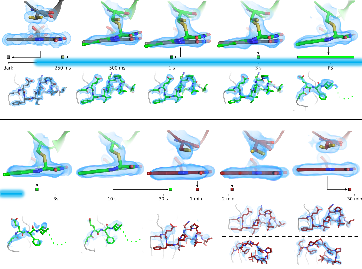
\includegraphics[width=\textwidth]{images/Introduction/Figure6_LOV2.pdf}
    \hfill
    \caption{Time-resolved structural changes in a LOV2 domain over 4 orders of time magnitude (from 63 ms to 27 min). The sequence starts with the dark state, which then proceeds to a steady-state equilibrium with the light state under continuous illumination (light blue on the timeline). After illumination has been stopped, the light state relaxes back to the dark state, yet in a different crystallographic state. The higher part of each structure features the cysteine residue and the FMN chromophore that engage in a thioether bond, the lower part represents the C-terminal part.}
    \label{fig:Figure6}
\end{figure}

\subsection{Monitoring of light-state relaxation by a time-resolved single crystal oscillation approach}
The endpoint of the experiment described in the previous section is the establishment of a steady-state equilibrium in a crystal of LOV2. The relatively slow decay time of the light state (Fig. \ref{fig:Figure4} (b)) prompted our group  to monitor how it relaxed by taking advantage of the fast acquisition rate of a Dectris EIGER X 4M detector and recording full oscillation data sets in only 1.2 s [400 images of 0.3° rotation (120° total rotation) and 3 ms acquisition time] on different crystals at various time points after termination of the illumination (Chapter \ref{chap:slowprot}), \cite{aumonierSlowProteinDynamics2022}). The structure of the first time point (t <0,i.e. under constant illumination; the last structure in the first timeline in Fig. \ref{fig:Figure6}) is that of LOV2 in a steady-state equilibrium composed predominantly of the light state and characterized by disorder of the C-terminus of the protein. As soon as the illumination is stopped, the occupancy of the thioether bond starts to decrease and electron density starts to build up on the C-terminus (the first three structures in the second timeline in Fig. \ref{fig:Figure6}). Shortly after 60 s, the diffraction data cannot be unambiguously reduced in a tetragonal space group but only in an orthorhombic space group, revealing the formation of a non-crystallographic dimer, which differs in the conformation of its C-terminus. The C-terminus of one monomer (upper row) folds into the helical conformation adopted in the dark-state structure at the beginning of the experiment, i.e. without any illumination, while that of the other monomer (lower row) eventually folds into a hook-shaped conformation (the final two structures in the second timeline). The whole relaxation is achieved 27 min after the end of illumination. This work constitutes a TR-MX study of a phenomenon occurring on a timescale of minutes to tens of minutes, which was probed with a time resolution of 1.2 s, demonstrating the feasibility of slow time-resolved diffraction studies on single crystals.

\section{Other light-activatable proteins}\label{sec:otherlighttrig}

\subsection{Photoactive Yellow Protein (PYP)}\label{sec:PYP}
PYP is a cytosolic blue-light photoreceptor from the phototrophic bacterium \textit{Halorhodospira halophila} and is implicated in negative phototaxis. It uses a 4-hydroxycinnamic acid molecule as a chromophore. Because PYP became the hallmark of time-resolved Laue crystallography, it was naturally chosen as one of the first targets to be investigated by TR-SFX. The remaining gaps in the structural understanding of its photoreaction were the events surrounding the cis/trans isomerisation step, which was expected to take place in the hundreds of femtoseconds regime, much shorter than the 100 ps time resolution of Laue crystallography. The first TRSFX study aimed to compare the quality of the produced difference electron-density maps with those obtained by Laue crystallography \parencite{tenboerTimeresolvedSerialCrystallography2014}. To this end, the well defined snapshots at 1 ms (corresponding to the most visible changes ascribed to the pR1 and pR2 states of the photocycle; that is, the movement of the S atom of the thioether bond linking the chromophore to the protein) and 10 ns (corresponding to a more challenging situation in which the three intermediate states ICT,pR1 and pR2 coexist and their deconvolution thus requires particularly good-quality data) were later chosen \parencite{pandeFemtosecondStructuralDynamics2016}. In a second step, the 142-1023 fs time domain was sampled to visualize the series of events leading to, and following, cis/trans isomerisation, which is proposed to occur between 500 and 650 fs. An additional time point at 3 ps served to characterize the fully relaxed intermediate. Overall, these studies have completed the structural description of the full PYP photocycle \textit{in crystallo}, which starts with light-induced chromophore isomerisation and proceeds to hydrogen-bond network reorganization. This eventually leads to the unfolding of two N-terminal helices, which constitutes the signalling state of the photoreceptor.

\subsection{Photoenzymes}\label{sec:photoenzymes}

For a long time, only two types of light-driven enzymes (photoenzymes) had been recognized as such: photolyases, which are DNA-repair (deoxyribonucleic acid) enzymes that convert pyrimidine dimers into a pair of pyrimidine bases under exposure to UV light \parencite{sancarStructureFunctionDNA2003}, and light-dependent protochorophyllide oxidoreductase (LPOR), which catalyses one of the last steps in chlorophyll biosynthesis \parencite{heyesMakingLightWork2005}. These two canonical photoenzymes were later joined by fatty-acid photodecarboxylase (FAP), which uses blue light to convert fatty acids to hydrocarbons \parencite{santoniHierarchicalClusteringMultiplecrystal2017}. Since the crystal structure of LPOR has been solved in the presence of the NADPH cofactor but without the substrate \parencite{zhangStructuralBasisEnzymatic2019}, time-resolved studies of its mechanism will have to wait until suitable crystals can be grown. The enzymatic photoenzyme of FAP has been studied by a wealth of biophysical techniques, including both cryo-trapping and time-resolved crystallographic approaches \parencite{sorigueMechanismDynamicsFatty2021}. The TR-SFX experiment probed events occurring 20 ps to 2 ms after light excitation. For photolyases, the mechanism of photoreduction of the FAD cofactor, which amounts to enzyme activation before the catalysis of damaged DNA repair can happen, was first deciphered by TR-SFX for a CPD (cyclobutane pyrimidine dimer) photolyase \parencite{maestre-reynaSerialCrystallographyCaptures2022} and by TR-SSX for a (6-4) photolyase \parencite{celliniStructuralBasisRadical2022}. In a second step, the whole repair mechanism of a CPD lesion by a photolyase was revealed from picoseconds to hundreds of microseconds \parencite{maestre-reynaVisualizingDNARepair2023a,christouTimeresolvedCrystallographyCaptures2023a}. It consists of the transfer of one electron from the FAD cofactor to the damaged DNA, the sequential breaking of two covalent bonds, the rearrangement of the various chemical groups involved in the reaction and, finally, the back-flipping of the two repaired DNA bases, which leads to dissociation of the enzyme-DNA complex. The complex analysis scheme we developed for that study will be detailed in Chapter \ref{chap:MmCPDII}.

\subsection{Photosystems and photoreaction centers}\label{sec:Photosystems}

A loosened definition of a photoenzyme may also apply to other systems \parencite{bjornPhotoenzymesRelatedTopics2018}. For instance, Photosystem II, the large membrane-protein complex that is responsible for the splitting of water during photosynthesis, has been extensively studied by (TR-)SFX, most notably because of the extreme sensitivity of its manganese cluster to X-ray-induced reduction precluding reliable (TR-)MX studies at synchrotrons. After an initial low-resolution TR-SFX study suggesting an elongation of the cluster \parencite{kupitzSerialTimeresolvedCrystallography2014}, a markedly higher resolution study uncovered structural changes occurring 10 ms after the sequential absorption of two photons, suggesting the formation of an oxo-bridge with the cluster \parencite{sugaLightinducedStructuralChanges2017}. The chemical nature of this bridge could later be precisely assessed as an oxyl/oxo species thanks to the higher resolution enabled by a cryo-trapping approach \parencite{sugaOxylOxoMechanism2019}. The full redox cycle of PSII (Kok’s clock) was first investigated by a TR-SFX study using multiple excitation schemes and varied time delays \parencite{kernStructuresIntermediatesKok2018}, and then by a more recent study which focuses on the last steps of the redox cycle \parencite{bhowmickStructuralEvidenceIntermediates2023}. The ultrafast events underlying the electron transfer (ET) after light absorption by a bacterial photosynthetic reaction centre was also investigated by TR-SFX\parencite{dodsUltrafastStructuralChanges2021}.

\subsection{Phytochromes}

Phytochromes are red and far-red light photoreceptors whose kinase activity is implicated in key cellular processes such as growth, germination, heat and light sensing, and phototropism in plants and fungi \parencite{chengPhytochromeSignalingNetworks2021}, photoprotection in nonphotosynthetic bacteria \parencite{davisBacteriophytochromesPhytochromeLikePhotoreceptors1999} and the synthesis of the photosynthetic apparatus in photosynthetic bacteria \parencite{giraudBacteriophytochromesAnoxygenicPhotosynthetic2008}. The structure of the chromophore-binding domain of bacteriophytochrome from \textit{Deinococcus radiodurans} (DrBph) revealed that the biliverdin chromophore is covalently bound to the PAS domain and inserted within the GAF domain \parencite{wagnerLightsensingKnotRevealed2005}. This first structure of truncated phytochrome paved the way for structural studies to understand the conversion between the red-absorbing Pr and far-red-absorbing Pfr states of the photoreceptor. Using a longer construct of DrBph that includes the additional phytochrome-specific domain PHY, Takala and coworkers showed that the GAF and PHY domains were separated by a structural element formed of two short \textBeta-strands belonging to the PHY domain: the PHYtongue. Using the ‘frozen equilibrium’ cryo-trapping strategy, they revealed that the light-induced Pr-to-Pfr conversion consists of the refolding of the tongue into an \textalpha-helix \parencite{takalaSignalAmplificationTransduction2014}. The same team attempted to visualize the details of the transition by TR-SFX by recording time points 1 and 10 ps after light excitation \parencite{claessonPrimaryStructuralPhotoresponse2020}. This study demonstrated that the twist of the D ring upon light-induced isomerisation of the chromophore drives a sequence of events (dissociation of the pyrrole water molecule and movement of the A ring and of an aspartate residue) that ultimately leads to ultrafast backbone movement and thus to destabilization of the PHY-tongue. They also performed a TR-SFX study on a different bacteriophytochrome from the myxobacterium Stigmatella aurantiaca at the later time points of 5 ns and 33 ms \parencite{carrilloHighresolutionCrystalStructures2021}. They observed a more pronounced isomerisation of the chromophore and displacement of the PHY domain both through the PHY-tongue and the long \textalpha-helix connecting the GAF and PHY domains.

\subsection{Photoswitchable fluorescent proteins}
The function of a fluorescent protein (FP) is to absorb photons around a certain energy (centred around the maximum peak of its absorption spectrum) using its chromophore, which is promoted to an excited state and then returns to the ground state by re-emitting secondary photons of lower energy. The efficiency of an FP is quantified by the ratio of emitted photons to absorbed photons, which is called the fluorescence quantum yield QY (0 < QY < 1). Deexcitation from the excited state occurs via radiative and nonradiative pathways, and the latter are minimized in an efficient FP. As a consequence, the chromophore of an efficient FP is constrained by a rigid environment, and thus the mechanism of fluorescence does not rely on atomic movements that could easily be observed by TR-SFX during the fluorescence lifetime, which is of the order of several nanoseconds. However, there is a class of FPs whose complex spectroscopic properties rely on the transformation of the chemical nature of the chromophore via isomerisation or covalent-bond breakage: the phototransformable FPs (PTFPs). The study of their phototransformation mechanism is possible by TR-SFX. The first example of a PTFP to be studied was the reversibly photoswitchable protein rsEGFP2 \parencite{coquelleChromophoreTwistingExcited2018}. Crystals of rsEGFP2 in the (non-fluorescent) off-state were excited with a 400 nm femtosecond laser, and data collection was performed 1 and 3 ps later. At 1 ps after laser excitation the chromophore exhibits a mixture of two conformations: one planar close to that of the off-state (model P) and one twisted halfway between the configurations of the off- and on- states (model T). At 3 ps model P has relaxed and there is a mixture of model T and a conformation resembling the onstate. A second study probed a later time point at 10 ns to validate that chromophore isomerisation has occurred on this timescale \parencite{woodhousePhotoswitchingMechanismFluorescent2020}. Another group chose the same protein but with a chemically modified chromophore, in which a Cl atom has been added to the terminal ring, in order to use TR-SFX to investigate whether the chromophore isomerisation process occurs via the hula-twist or the onebond-flip pathway \parencite{fadiniSerialFemtosecondCrystallography2023}. Structural changes were probed 300 fs, 600 fs, 900 fs, 5 ps, 100 ps and 1 ms after laser excitation and first revealed that the Cl atom remains on the same side of the ring, demonstrating that isomerisation occurs through the hula-twist mechanism. Surprisingly, traces of the isomerized chromophore are already present at 300 fs. Also, a constrained intermediate builds up at 600 fs and then decays by 5 ps. isomerisation is then completed by 100 ps. A TR-SSX study was applied to another reversibly photoswitchable FP (rsFP), rsEospa, to probe the nature of the isomer produced during 1 ms of exposure to laser illumination for different isomers at pH values ensuring different protonation states \parencite{baxterObservationCationChromophore2022}. Finally, the same group as in the two latter examples evolved the rsFP EosFP into rsKiiro with improved photochemical properties (which include a high photochemical quantum yield of photoisomerisation) and diffraction resolution at room temperature (better than 1.5 \AA\ for microcrystals at XFELs) in order to amplify the signal contained in the Fourier difference maps. They used a two-pulse pump-dump excitation scheme (at 400 and 515 nm, respectively) to investigate whether the ultrafast (subpicosecond) protein dynamics form part of the photoisomerisation process. By using a single-pulse excitation scheme as a control, they were able to disprove this \parencite{hutchisonOpticalControlUltrafast2023}.

\section{Examples of TR-MX studies of biological systems relying on ligand or substrate delivery}\label{sec:diffusion}

TR-SX experiments initially focused on photoreactions, for which reaction triggering is initiated with a visible laser pulse, thus minimally complicating the sample environment. In order to broaden the range of targets, sophisticated substrate/ cofactor-delivery systems had to be developed and fitted within a crowded experimental setup. There are essentially two ways of initiating a substrate/cofactor-dependent reaction. The first and more versatile method relies on the diffusion of a small molecule within the channels of a protein crystal, either by mixing of solutions (for a flow of crystals) or soaking (for a stationary crystal, to which a cofactor/substrate solution is delivered). It is worth noting that the diffusion of substrates and cofactors into microcrystals occurs on the high-microsecond, low-millisecond timescale at best \parencite{makinenReactivityCryoenzymologyEnzymes1977,schmidtMixInjectReaction2013,pandeyObservationSubstrateDiffusion2021}, which prevents access to fast to ultrafast events. Various types of sample delivery setups have been developed. Firstly, a microfluidic-based mixing capacity can be positioned upstream of a viscous or liquid sample injector \parencite{wangDoublefocusingMixingJet2014, calveyMixingInjectorEnables2016, dopplerCoflowInjectionSerial2022}. Samples can be probed within the microfluidic device itself, for instance, the 3D-printed microfluidic chip 3D-MiXD \parencite{monteiro3DMiXD3DprintedXraycompatible2020}. Alternatively, crystals can be deposited onto a moving tape (TapeDrive system) after rapid liquid mixing has occurred (this setup was used in Part \ref{part:T-Cer}, and described in Section \ref{sec:presenting_tpd_P11}, \cite{beyerleinMixanddiffuseSerialSynchrotron2017, zielinskiRapidEfficientRoomtemperature2022}). The BITS (comBination of Inject-and-Transfer System) sample-delivery method combines the advantages of the sample-injection and fixed-target approaches by injecting a pre-mixture of crystals and solutions through a needle tip onto an ultraviolet ozone-treated polyimide film held on a translation stage, horizontal and vertical motions of which permit scanning of the whole film by the X-ray beam \parencite{leeUpgradedCombinedInjectandTransfer2022}. While these techniques rely on the mixing of solutions, an alternative consists of delivering droplets of substrate/cofactor solution directly onto a crystal sitting on a sample holder, which amounts to crystal soaking. In the first such example, crystals are loaded onto a fixed-target chip onto which a substrate/cofactor solution is sprayed: this technique has been named LAMA (Liquid Application Method for time-resolved Analyses; \parencite{mehrabiLiquidApplicationMethod2019}. Of note, this approach requires the installation of a humidity-control chamber around the sample environment. Similarly, the drop-on-drop method consists of delivering bursts of picolitre-sized substrate/cofactor drops onto crystals positioned on a moving tape \parencite{butrynOndemandDropondropMethod2021}. All of these techniques have primarily been developed for room-temperature time-resolved applications, but they could be adapted for cryo-trapping approaches for timescales above the typical flash-cooling time (\textasciitilde1-100 ms depending on the crystal size) using the MMQX (millisecond mix-and-quench crystallography; \cite{clingerMillisecondMixandquenchCrystallography2021} and spitrobot \parencite{mehrabiMillisecondCryotrappingSpitrobot2023} approaches.

\begin{figure}[H] %bt!]
    \centering
    \noindent 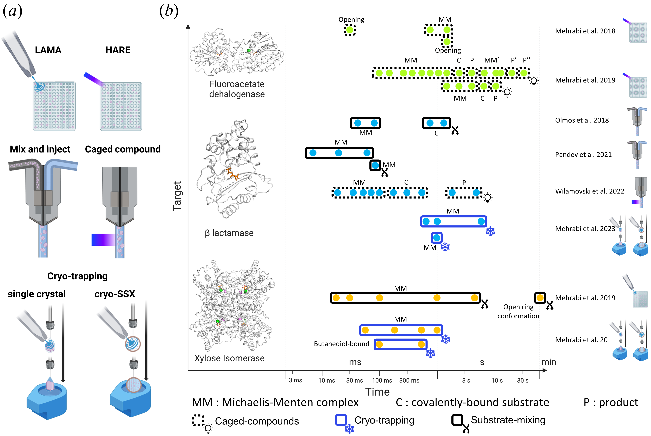
\includegraphics[width=\textwidth]{images/Introduction/Figure7_diffusion.pdf}
    \hfill
    \caption{Diffusion-based time-resolved experiments. (a) Strategies enabling the initiation of a reaction by the diffusion of a substrate or a cofactor. (b) Overview of studies conducted on emblematic targets: fluoroacetate dehalogenase (depicted using PDB entry 5k3a; \cite{mehrabiLiquidApplicationMethod2019}), \textBeta-lactamase (depicted using PDB entry 7bh5; \cite{butrynOndemandDropondropMethod2021}) and xylose isomerase (depicted using PDB entry 8aw8; \cite{mehrabiMillisecondCryotrappingSpitrobot2023}). Colour code: protein secondary structure, white; substrate, orange; ions, green (chloride ion), red [magnesium(II) ion] and lilac [manganese(II) ion].}
    \label{fig:Figure7}
\end{figure}

The second method, as already mentioned in Section \ref{sec:howtostart}, relies on the photo-induced cleavage of a protective group in a so-called ‘photocaged’ substrate/cofactor \parencite{monteiroUsingPhotocagingFast2021}. If the photocaged molecule has been co-crystallized or soaked with the crystals prior to the experiment, the limiting factor here is not the small-molecule diffusion time through the solvent channels but the ligand-release time after the decaging light pulse.

Three main examples of diffusion-based reactions studied by TR-SX have focused attention over the past years. The enzyme fluoroacetate dehalogenase (FAcD) was first used to develop the ‘hit-and-return’ (HARE) method, which enables TR-SSX for time resolutions ranging from milliseconds to tens of seconds (Fig. \ref{fig:Figure7}7a; \cite{schulzHitandreturnSystemEnables2018}). Using caged fluoroacetate, the binding of its natural substrate by FAcD was studied using an experimental protocol that minimizes the data-acquisition time. At 30 ms, active-site opening is observed for one of the two monomers in the asymmetric unit. Between 752 and 2052 ms, the substrate-bound state, or Michaelis-Menten (MM) complex, is progressively populated. At 2052 ms, the active site of the second monomer starts to open as well (Fig. \ref{fig:Figure7}\textit{b}). Using the same approach, the same authors greatly extended the time range to \textasciitilde30 s to observe four catalytic cycles of enzyme turnover (three for monomer A and one for monomer B; \cite{mehrabiLiquidApplicationMethod2019}. For monomer A, the MM complex is observed between 188 and 2052 ms. At 2256 ms, the formation of a covalent intermediate (C) is observed. The product (P) is observed at 4512 ms and is released by 6156 ms. Two further cycles are subsequently observed. A different kinetic is observed for monomer B, suggesting that substrate access to the active site is allosterically controlled.

The LAMA technique (Fig. \ref{fig:Figure7}\textit{a}) was developed by the same authors using xylose isomerase (XI; \cite{mehrabiTimeresolvedCrystallographyReveals2019}. A solution of glucose was sprayed onto XI crystals sitting in the wells of a fixed-target chip and diffraction data sets were recorded at approximate time points of 15 ms, 30 ms, 100 ms, 1 s, 4.5 s and 60 s. The binding of the substrate is maximal at 100 ms. XI appears to be idle at 1 and 4.5 s, but the glucose ring is observed to be open at 60 s, demonstrating enzymatic activity (Fig. \ref{fig:Figure7}\textit{b}). During this PhD, LAMA, in combination with HARE was used on the T-REXX beamline, to study the isomerisation of a fluorescent protein (Section \ref{sec:T-REXX}) XI was also used to demonstrate the cryotrapping capability of the spitrobot \parencite{mehrabiMillisecondCryotrappingSpitrobot2023}. They first showed that the cryoprotectant 2,3-butanediol binds preferentially to glucose within 50 and 500 ms (i.e. before flash-cooling). In the absence of 2,3-butanediol, they were able to observe full occupancy of glucose binding at 50, 250, 500 and 1000 ms.

Next, various antimicrobial resistance proteins of the \textBeta-lactamase (\textBeta-lac) type were studied using many of the abovementioned techniques and methods. Olmos and coworkers used an mix-and-inject approach to visualize the binding of an antibiotic to \textBeta-lac (time points of 30 and 100 ms) and its subsequent cleavage (500 ms and 2 s) \parencite{olmosEnzymeIntermediatesCaptured2018}. A follow-up study observed binding at shorter time points for the same antibiotic (5, 10 and 50 ms) and that of an inhibitor at 66 ms \parencite{pandeyObservationSubstrateDiffusion2021}. A caged Zn2+ approach was used at BioCARS with Laue serial diffraction to probe ten time points of the reaction of a metallo-\textBeta-lactamase with the antibiotic moxalactam from 20 to 4000 ms \parencite{wilamowskiTimeresolvedVlactamCleavage2022}. For the five time points between 20 and 100 ms, substrate binding is observed (Fig. \ref{fig:Figure7}\textit{b}). From 150 to 500 ms, a hydrolysed moxolactam intermediate is observed. The product then relaxes within the active site by 2 s and remains in place until 4 s at least. Finally, an activity-impaired \textBeta-lac was also used to test the spitrobot, which allowed the authors to characterize the inhibitor-bound structure by cryo-SSX from microcrystals (flash-cooled after 1 s) and the covalent binding of ampicillin in single crystals at time points of 0.5, 1 and 5 s \parencite{mehrabiMillisecondCryotrappingSpitrobot2023}.

\section{Aim of this thesis}

TR-MX experiments rely on data-collection schemes which are demanding in beamtime, they use sophisticated sample environments and stringent sample requirements. Processing, analysing and interpreting TR-MX data is also challenging and often requires validation of the results with complementary techniques. Because of these requirements, it remains the domain of a few, specialised groups. Further, TR-MX has yet to truly extend past light-activated systems, into the realm of reactions activated by the diffusion of a substrate (including proton or electron donors). There is also a deficit in 'fast-to-slow' TR-MX experiments sampling the \textmu s to minutes time-domain despite them being theoretically more manageable than ultrafast experiments which overall require greater amounts of sample and cannot take place at the more accessible synchrotron beamlines. Importantly, fast-to-slow TR-MX is better adjusted to the timescale at which most enzymatic reactions occur \parencite{bar-evenModeratelyEfficientEnzyme2011}.

Throughout this PhD, we encountered the aforementioned challenges within several of our own projects as well as in collaboration and developed methods and tools to address them. This thesis is structured in four parts, three of which correspond to the three biological projects of this PhD, and the last presents the tools and methods developed to make \textit{ic}OS more accessible as a technique complementing TR-MX. In Part \ref{part:T-Cer}, the pH-driven isomerisation of a cyan fluorescent protein is characterised through the use of many novel diffusion-based TR-MX environments. In Part \ref{part:LOV2}, we designed an inexpensive slow TR-MX method to probe the decay of the signalling state of a plant blue light sensor. Part \ref{part:Photolyase-Cryptochromes} presents the tools produced for analysis of TR-MX data, and the results of studies of the mechanism of DNA repair by a photolyase and signalling mechanism of a closely related cryptochrome in a large collaborative framework, as well as the continued evolution of the TR-SOX (Section \ref{sec:LOV2_TR-SOX}) technique. Finally, Part \ref{part:Spectro} presents the tools developed for \textit{ic}OS in parallel to TR-MX, which is illustrated by the study of a redox-switching iron transporter protein from a microalgae.



}
\counterwithin{section}{chapter}
\pagebreak
\part{Visualising pH-induced chromophore isomerisation of a Cyan Fluorescent Protein: kinetic vs time-resolved crystallography}\label{part:T-Cer}
\counterwithout{section}{chapter}
	{\section{A brief history of the Cyan Fluorescent Proteins}\label{sec:prior_T-Cer}
The discovery of the green fluorescent protein (GFP) in the jellyfish \textit{Aequorea victoria} \parencite{shimomuraExtractionPurificationProperties1962}, followed by its cloning \parencite{prasherPrimaryStructureAequorea1992} and the demonstration that it could be used as a marker for gene expression \parencite{chalfieGreenFluorescentProtein1994}, opened the way to a vast array of imaging techniques at the core of contemporary biology. A single mutation of the original \textit{Aequorea victoria}  protein, on position 65:S65T, simplified the fluorescent spectrum of the GFP by simplifying its fluorescence spectrum from two excitation peaks to one single peak at 488 nm, with enhanced amplitude \parencite{heimImprovedGreenFluorescence1995}. The structure of this mutant was later solved, revealing that the GFP consisted of a \textbeta-barrel structure, in which amino acids 65,66 and 67 undergo auto-catalytic cyclization of their backbone to form the chromophore of the protein (\cite{ormoCrystalStructureAequorea1996} Fig. \ref{fig:FP_chromo}).
\begin{figure}[ht] %bt!]
    \centering
    \noindent 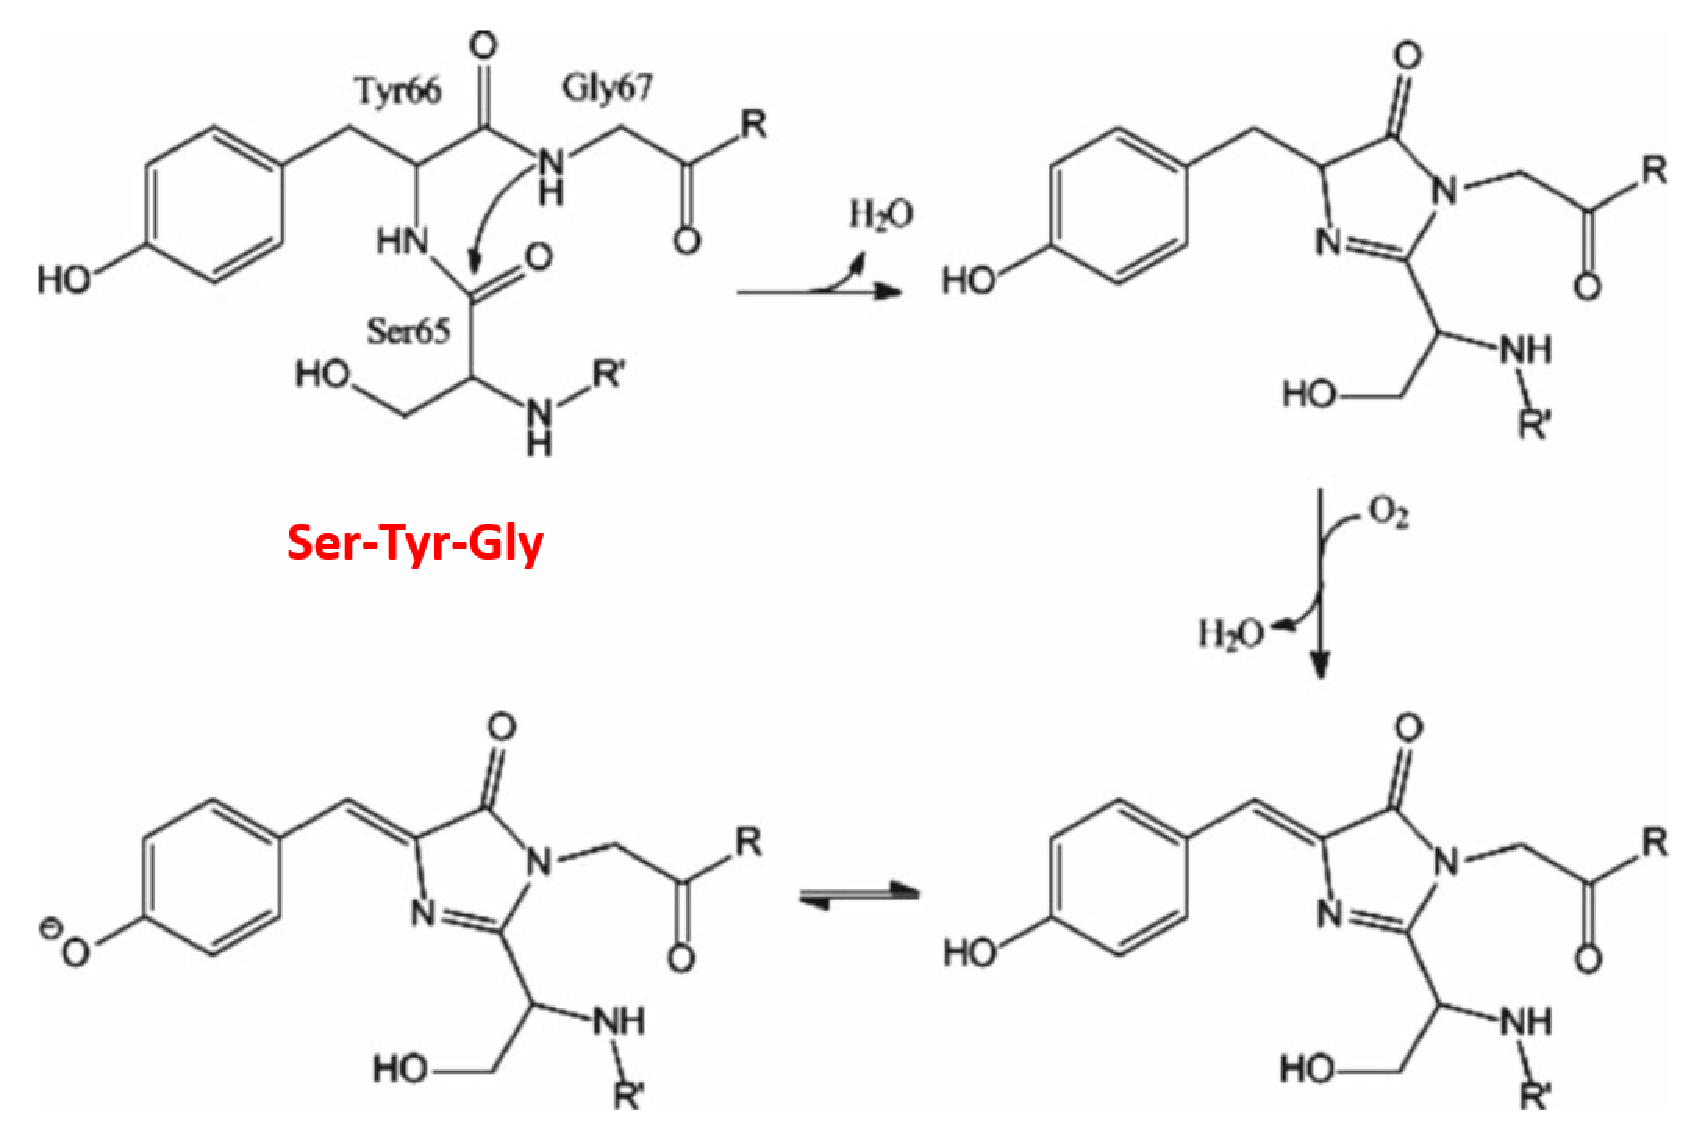
\includegraphics[width=0.6\textwidth]{images/T-Cer/GFP_autocatalytic_cyclisation.pdf}
    \hfill
    \caption{Autocatalytic cyclisation mechanism leading from a short peptide sequence (Serine-Tyrosine-Glycine) to a fluorophore. The mature, excitable chromophore of the GFP is in the anionic form. Figure reproduced from \cite{cannonRedoxSensitiveGreenFluorescent2009}}
    \label{fig:FP_chromo}
\end{figure}
The first Cyan Fluorescent Protein (CFP) was obtained by combining mutation S65T of the GFP with Y66W: replacing the aromatic residue central to the chromophore triad (\cite{heimWavelengthMutationsPosttranslational1994}, Fig. \ref{fig:CFP_isomere}). A few mutations were needed to accommodate the bulk of the bigger tryptophan, leading to the enhanced CFP (ECFP) \parencite{heimWavelengthMutationsPosttranslational1994}. However, the quantum yield of the ECFP remained low. Building on the crystal structure of the ECFP, a series of beneficial mutations were introduced, creating Cerulean \parencite{rizzoImprovedCyanFluorescent2004}. 

\begin{figure}[ht] %bt!]
    \centering
    \noindent 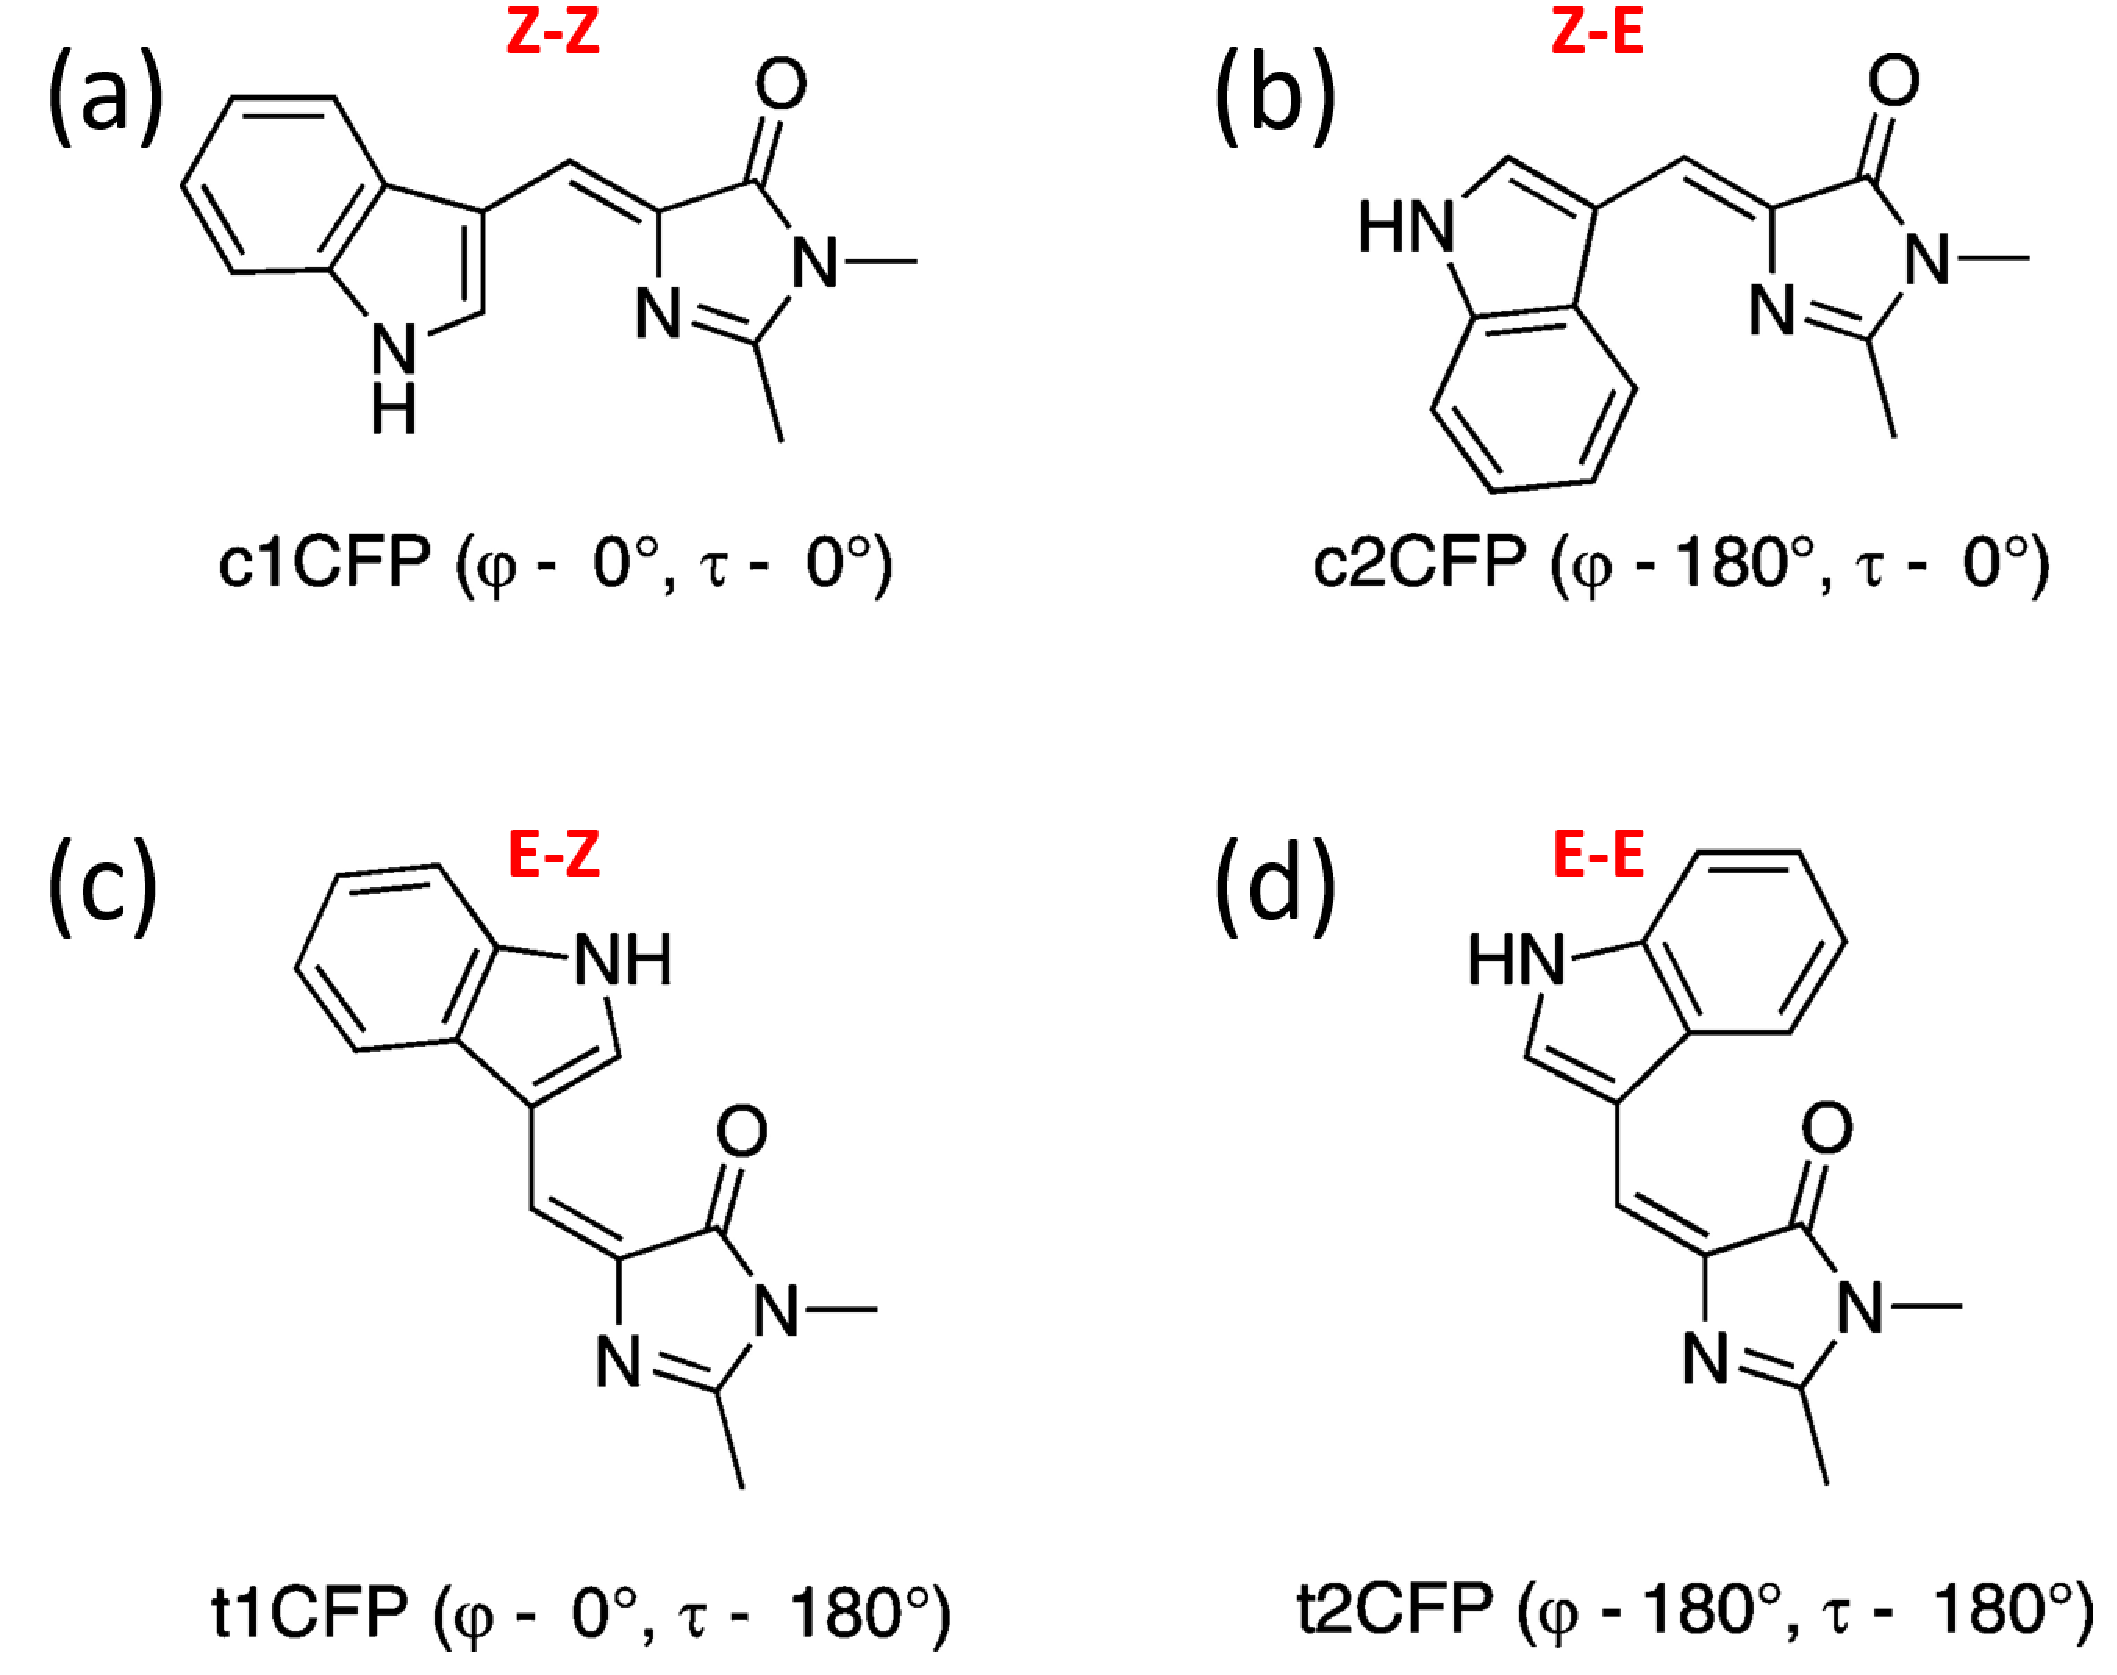
\includegraphics[width=0.8\textwidth]{images/T-Cer/CFP_isomeres.pdf}
    \hfill
    \caption{The CFP chromophore, obtained from the Threonine-Tryptophan-Glycine sequence, and its different stereochemical configurations as calculated from Density Function Theory. (a) configuration Z-Z, (b) configuration E-Z, (c) configuration E,Z and (d) configuration E-E. Figure reproduced from \cite{volianiCisTransPhotoisomerizationFluorescentProtein2008}}
    \label{fig:CFP_isomere}
\end{figure}
The first structure of Cerulean, obtained from a crystal grown at acidic pH (\cite{maloXrayStructureCerulean2007}, right panel in Fig. \ref{fig:Cerulean_pH} (a)) revealed that its chromophore adopted the configuration Z,E (Fig. \ref{fig:CFP_isomere} (b)) while the first structure of Cerulean obtained from crystals grown at neutral pH  (\cite{lelimousinIntrinsicDynamicsECFP2009}, left panel in Fig. \ref{fig:Cerulean_pH} (a)) later revealed a chromophore in configuration Z,Z (Fig. \ref{fig:CFP_isomere} (b)), where the chromophore is stabilised by a hydrogen-bond (H-bond) network encompassing S205, E222, anchoring the chromophore by its indole ring and by the carbonyl of S65 (the first amino-acid in the chromophore triad) (Fig. \ref{fig:Cerulean_pH} (b)).  The group of Antoine Royant generated variants to explore possible fluorescence-enhancing mutations. The fluorescence of one such variant, T65A, was particularly sensitive to pH, with a fluorescence pKa between 5.5 and 6.0 (Fig. \ref{supfig:Fluo_T-Cer}) vs 4.7 for Cerulean \parencite{rizzoImprovedCyanFluorescent2004}.  Similar to all GFP-like proteins, T65A adopts a beta-barrel fold, with the chromophore positioned on the central strand (Fig. \ref{fig:overall}). 

\begin{figure}
    \centering
    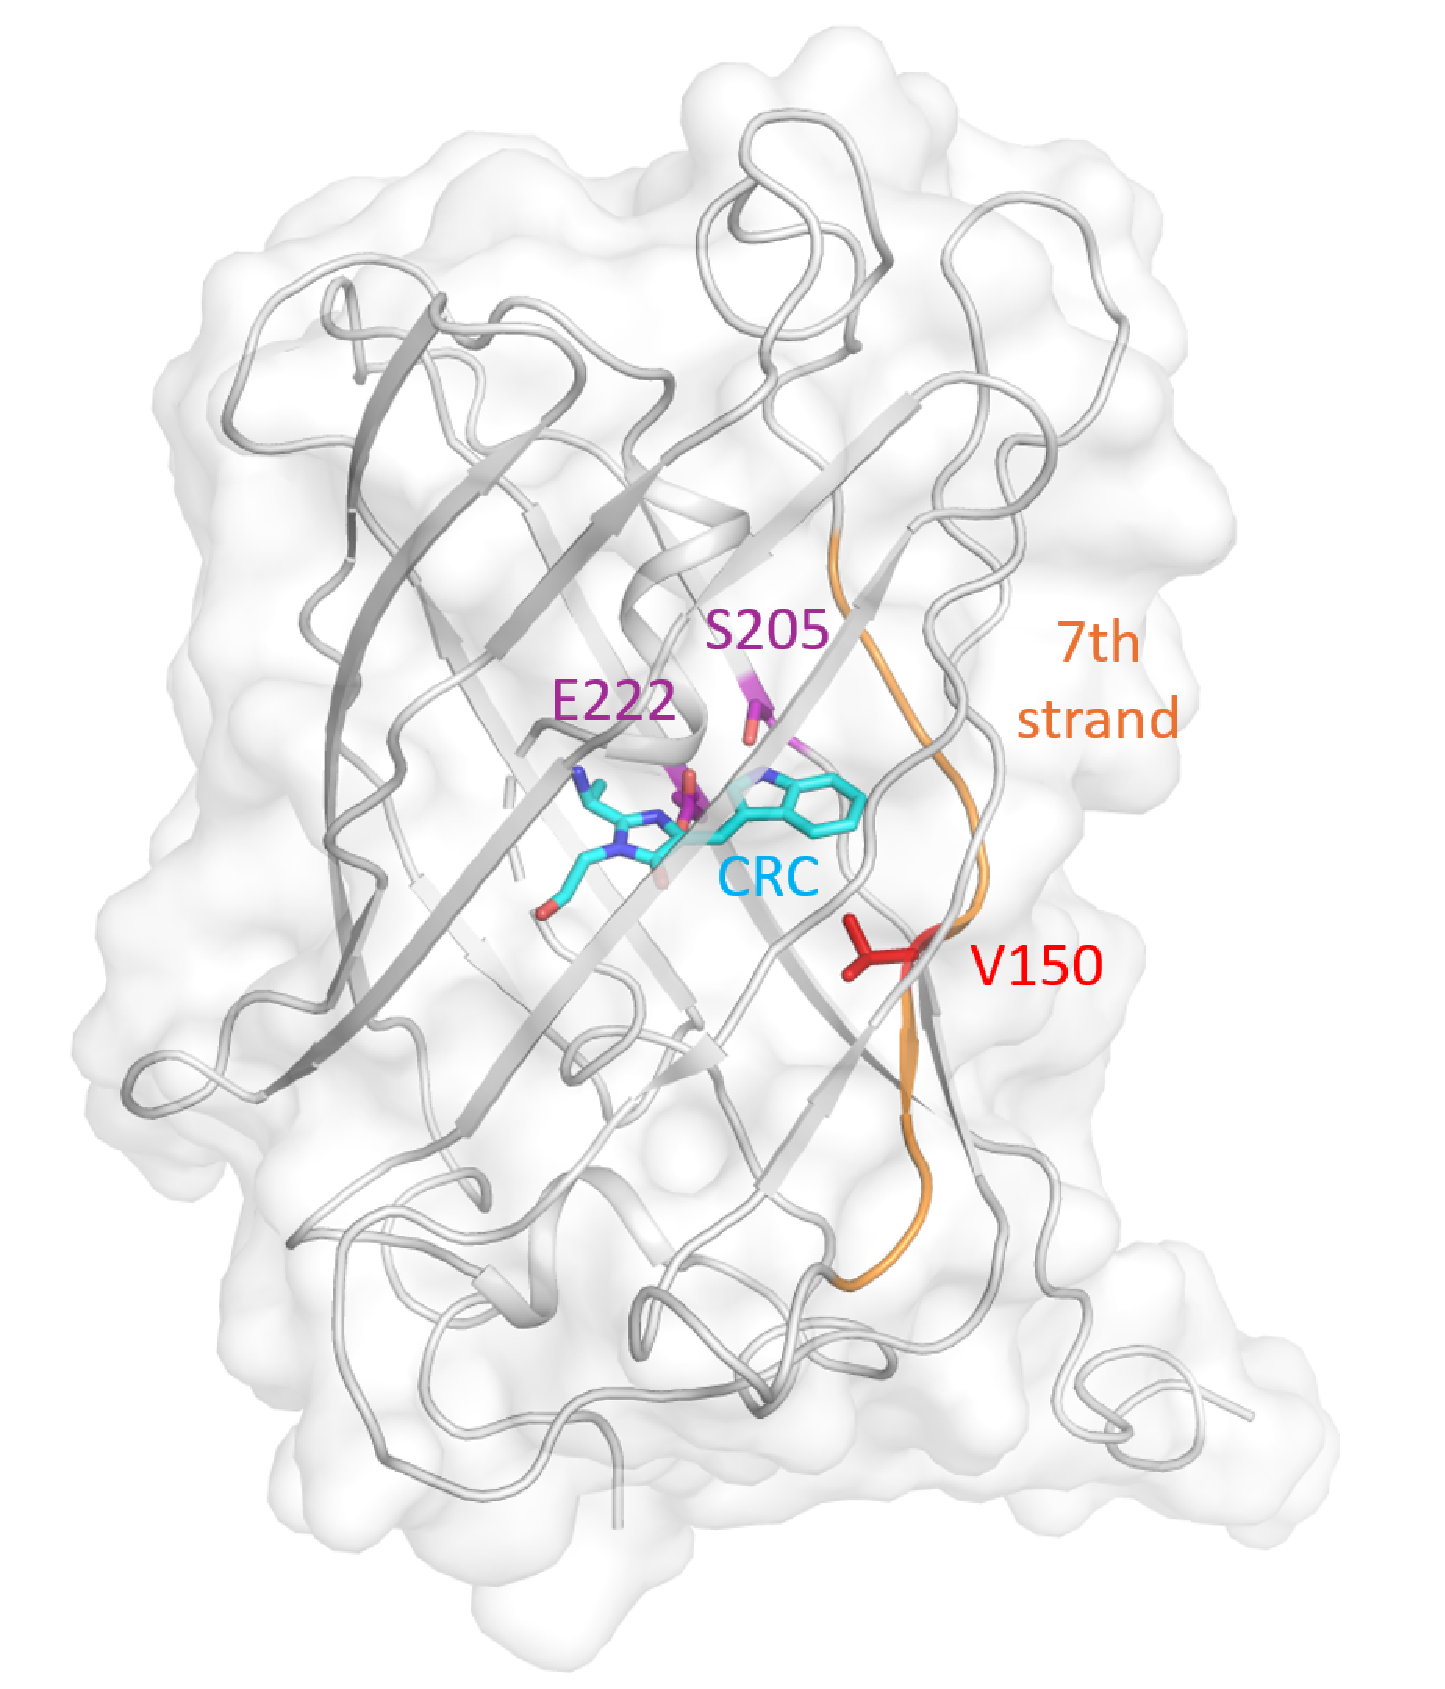
\includegraphics[width=0.7\textwidth]{images/T-Cer/Overall.pdf}
    \caption{Global view of the structure of the \textbeta-barrel structure of T65A/Twist-Cerulean variant of the Cerulean fluorescent protein. E222 and S205, involved in the H-bond network stabilising the chromophore at physiological pH, are coloured purple. V150 is coloured red and the 7\textsuperscript{th} strand of the \textbeta-barrel structure is coloured orange. }
    \label{fig:overall}
\end{figure}

Without the carbonyl from the threonine side chain in the first position of the chromophore triad, the H-bond network of the chromophore is only anchored by its indole ring (Fig. \ref{fig:Cerulean_pH} (b)). This is a potential explanation for the exacerbated sensitivity to pH of T65A: in its H-bond network, only one side of E222 is mobilised, and the entire network falls apart when E222 is protonated, whereas in Cerulean E222 conserves its H-bond with the side chain of T65, even at lower pH (Fig. \ref{fig:Cerulean_pH} (a), right panel). Once unanchored, the chromophore of T65A is free to de-excite vibrationally by rotation around its methylene bridge and, therefore, less likely to de-excite by emitting a fluorescence photon upon excitation \parencite{gotthardChromophoreIsomerStabilization2017a}. Strikingly, while the chromophore of Cerulean adopts the Z,E configuration at acidic pH (Fig. \ref{fig:Cerulean_pH} (a)) via a rotation around the CG-CB bond of the methylene bridge, the chromophore of T65A adopts the E,Z configuration at lower pH (Fig. \ref{fig:Cerulean_pH} (b)), corresponding to a rotation around the CA2-CB bond of the methylene bridge.
\begin{figure}[H] %hbt!]
    \centering
    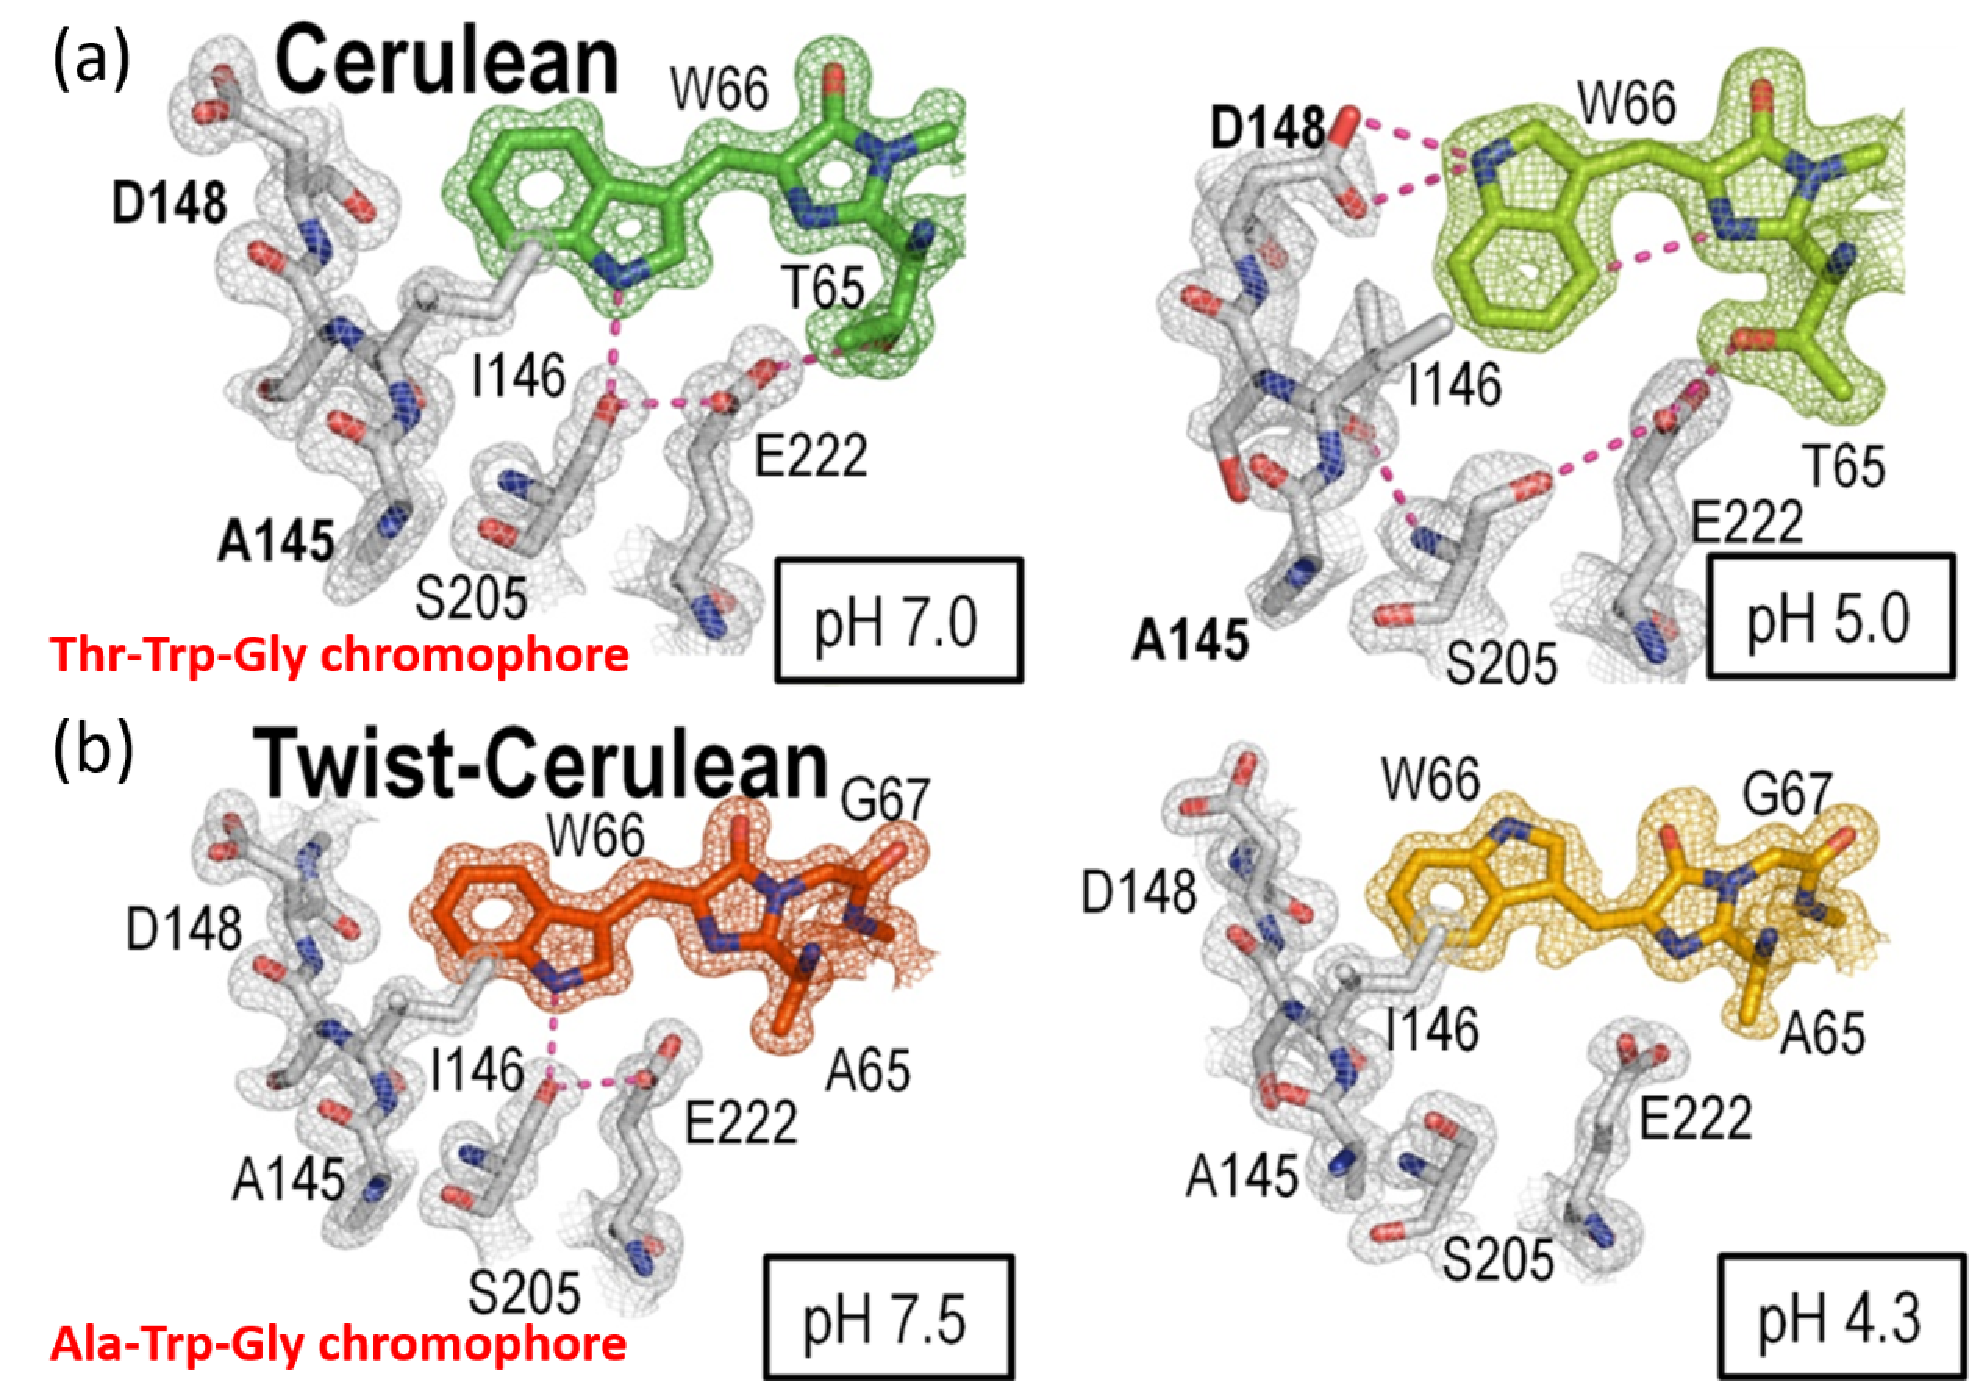
\includegraphics[width=\textwidth]{images/T-Cer/Cer-Tcer_pH.pdf}
    \hfill
    \caption{CFPs chromophore configuration at neutral and acidic pH \textbf{(a)} the cerulean fluorescent protein \textbf{(b)} the T-Cer variant. Structures collected and figures prepared by David von Stetten.}
    \label{fig:Cerulean_pH}
\end{figure}

As the pH drops from neutral to acidic, the transition from configuration Z,Z to Z,E for Cerulean, and Z,Z to E,Z for T65A is accompanied by a blue shift of their main UV-vis absorption band (Fig. \ref{fig:pH_TRspectroinsolution}, unpublished data from the team of Hélène Pasquier, Université Paris-Saclay).  When followed by time-resolved UV-vis absorption spectroscopy in solution after the protein at neutral pH (Tris, pH 8.0) is mixed with an acidic pH buffer (sodium acetate, pH 5.0), the isomerisation process occurs over several hours in Cerulean (Fig. \ref{fig:pH_TRspectroinsolution} (a)). In stark difference, the absorption band of T65A blue loses its two peaked structure and blue shifts in 80 ms (Fig. \ref{fig:pH_TRspectroinsolution} (b)) and remains stable afterwards (Fig. \ref{supfig:Fluo_T-Cer}). Its fast isomerisation earned it the nickname 'Twist-Cerulean" (T-Cer).
\begin{figure}[H] %hbt!]
    \centering
        \noindent 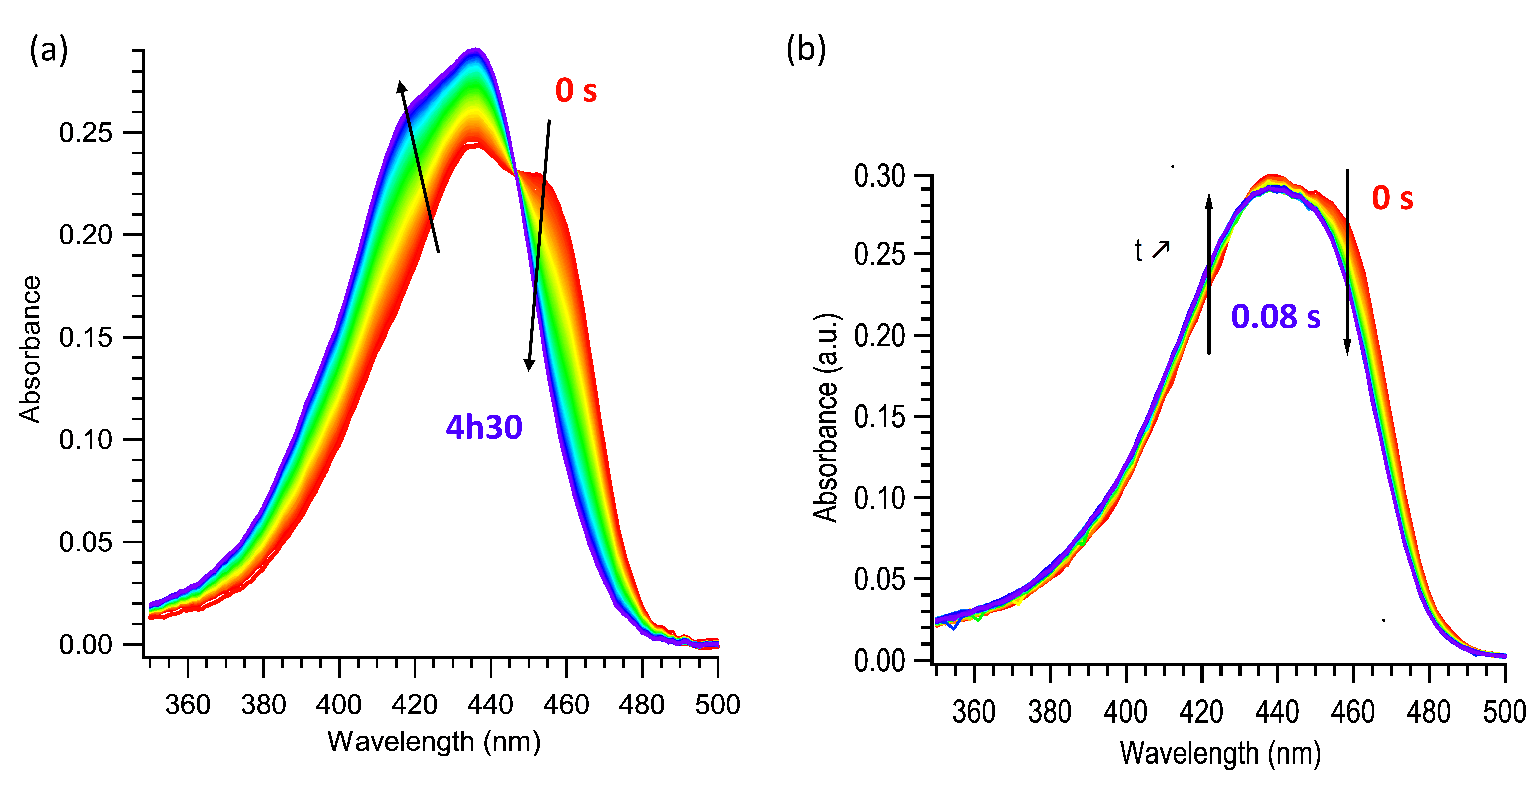
\includegraphics[width=\textwidth]{images/T-Cer/insolution_spectro_time.pdf}
    \hfill
    \caption{pH-drop-induced isomerization of the chromophore of Cerulean (a) and T-Cer (b), followed by in-solution absorption spectroscopy after the protein in a neutral pH buffer (Tris, pH 8.0) is mixed with an excess of acidic pH buffer (sodium acetate, pH 5.0) using a stopped-flow device. Spectra go from red (0 s) to blue (4h30 for Cerulean and 80 ms for T-Cer). Figure prepared by Helène Pasquier}
    \label{fig:pH_TRspectroinsolution}
\end{figure}
The surroundings of a fluorophore are tightly packed to maximize fluorescence efficiency. It is intriguing that the important configuration change from Z,Z to E,Z can happen so fast in such a cramped space. The configuration switch presumably occurs over a time scale (80 ms), perfectly matching the capability of the emerging TR-SSX beamlines (particularly beamline ID29 at the ESRF).  Further, at acidic pH, the chromophore of T-Cer adopts a configuration (E,Z) that had not previously been observed for tryptophan-based fluorophores, with altered spectroscopic properties which could serve as the backbone for a  pH-sensing fluorescent protein. 

\vspace{10mm}

Therefore, this project aims to structurally characterise the pH-drop-induced switch of from the reference configuration Z,Z to the novel configuration E,Z in T-Cer, on the \textmu s - s time-domain.

\subsection{List of structures}

Throughout the T-Cer project, several X-ray crystallography structures were determined; they are described in Table \ref{tab:structure-list} (at the end of the section), and will be presented in the coming sections. 
\clearpage
\begin{sidewaystable}[h]
    \begin{tabular}{c>{\centering\arraybackslash}p{0.02\linewidth}>{\centering\arraybackslash}p{0.03\linewidth}>{\centering\arraybackslash}p{0.1\linewidth}>{\centering\arraybackslash}p{0.07\linewidth}c>{\centering\arraybackslash}p{0.07\linewidth}>{\centering\arraybackslash}p{0.08\linewidth}>{\centering\arraybackslash}p{0.07\linewidth}>{\centering\arraybackslash}p{0.02\linewidth}>{\centering\arraybackslash}p{0.02\linewidth}>{\centering\arraybackslash}p{0.02\linewidth}}
         \hline
         Name & pH&   time-point (s)&Sample environnement&  temperature&  beamline &  construct&  precipitant &  resolution (\AA)&  \multicolumn{3}{c}{lattice parameters}\\
         \hline
         & &   &&  &  &  &  &  &  a&  b& c\\
         REF& 8&   &MX&  100 K&  ID30B-ESRF&  T-Cer&  PEG&  1.2&  50.9&  62.7& 69.4\\
         2D& 4&   &MX&  100 K&  ID30B-ESRF&  T-Cer&  PEG&  1.3&  51.6&  62.1& 64.6\\
         8D& 4&   &MX&  100 K&  ID30B-ESRF&  T-Cer&  PEG&  1.4&  51.5&  62.0& 64.5\\
         15D& 4&   &MX&  100 K&  ID30B-ESRF&  T-Cer&  PEG&  1.1&  51.3&  59.2& 64.1\\
         30D& 4&   &MX&  100 K&  ID30A3-ESRF&  T-Cer&  PEG&  1.4&  52.2&  62.6& 65.2\\
         REF-TPD-1& 8&   &Tape-drive&  220 K&  P11-DESY&  T-Cer&  PEG&  1.8&  51.7&  62.8& 70.7\\
         760MS-TPD-1& 8&   0.760&Tape-drive&  220 K&  P11-DESY&  T-Cer&  PEG&  1.8&  51.7&  62.8& 70.7\\
         REF-LAMA& 8&   &Fixed-target&  220 K&  P14-2-DESY&  T-Cer&  PEG&  1.7&  51.9&  62.7& 72.4\\
         3S-LAMA& 8&   3&Fixed-target&  220 K&  P14-2-DESY&  T-Cer&  PEG&  2.3&  50.9&  63.2& 66.0\\
         REF-TPD& 8&   &Tape-drive&  220 K&  P11-DESY&  T-Cer&  PEG&  2.0&  52.0&  63.0& 72.6\\
         3S-TPD-Ac& 8&   3&Tape-drive&  220 K&  P11-DESY&  T-Cer&  PEG&  1.9&  52.0&  63.7& 66.8\\
         8S-TPD-Ac& 8&   8&Tape-drive&  220 K&  P11-DESY&  T-Cer&  PEG&  2.1&  52.0&  63.7& 66.8\\
         300MS-TPD-Ci& 8&   0.300&Tape-drive&  220 K&  P11-DESY&  T-Cer&  PEG&  1.9&  52.0&  63.0& 72.6\\
         1S-TPD-Ci& 8&   1&Tape-drive&  220 K&  P11-DESY&  T-Cer&  PEG&  1.9&  52.0&  63.0& 72.6\\
         3S-TPD-Ci& 8&   3&Tape-drive&  220 K&  P11-DESY&  T-Cer&  PEG&  2.1&  52.0&  63.7& 66.8\\
         8S-TPD-Ci& 8&   8&Tape-drive&  220 K&  P11-DESY&  T-Cer&  PEG&  2.1&  52.0&  63.7& 66.8\\
         16S-TPD-Ci& 8&   16&Tape-drive&  220 K&  P11-DESY&  T-Cer&  PEG&  2.1&  52.0&  63.7& 66.8\\
         REF-TPD-ID29 & 8&   &Tape-drive&  220 K&  ID29-ESRF&  T-Cer&  PEG&  2.2&  51.5&  62.5& 71.0\\
         60S-TPD& 8&   60&Tape-drive&  220 K&  ID29-ESRF&  T-Cer&  PEG&  2.4&  53.0&  63.0& 66.0\\
         150S-CT-S& 8&   150&MX&  100 K&  ID23-2-ESRF&  T-Cer-s&  (NH\textsubscript{4})\textsubscript{2}SO\textsubscript{4}&  1.3&  51.9&  62.5& 66.2\\
         180S-RT-S& 8&   180&MX&  220 K&  ID23-2-ESRF&  T-Cer-s&  (NH\textsubscript{4})\textsubscript{2}SO\textsubscript{4}&  2.2&  52.0&  63.7& 67.7\\
         REF-ALD& 8&   &ALD&  220 K&  PXI-SLS&  T-Cer-s&  (NH\textsubscript{4})\textsubscript{2}SO\textsubscript{4}&  2.2&  51.5&  62.5& 70.5\\
         150S-ALD& 8&   150&ALD&  220 K&  PXI-SLS&  T-Cer-s&  (NH\textsubscript{4})\textsubscript{2}SO\textsubscript{4}&  2.5&  51.6&  61.8& 66.2\\
         300S-ALD& 8&   300&ALD&  220 K&  PXI-SLS&  T-Cer-s&  (NH\textsubscript{4})\textsubscript{2}SO\textsubscript{4}&  2.7&  51.5&  61.1& 65.5\\
         8-V150A& 8&   &MX&  100 K&  BM07-ESRF&  T-Cer-s&  (NH\textsubscript{4})\textsubscript{2}SO\textsubscript{4}&  1.1&  51.1&  62.3& 69.4\\
         4-V150A& 4&   &MX&  100 K&  BM07-ESRF&  T-Cer-s&  (NH\textsubscript{4})\textsubscript{2}SO\textsubscript{4}&  1.3&  51.2&  62.6& 70.1\\
         10S-V150A& 8&   &MX&  100 K&  BM07-ESRF&  T-Cer-s&  (NH\textsubscript{4})\textsubscript{2}SO\textsubscript{4}&  1.0&  51.2&  62.4& 69.1\\
         \hline
    \end{tabular}
    \caption{List of structures of T-Cer and T-Cer-s}\label{tab:structure-list}
\end{sidewaystable}

\section{Preparing the TR-SSX experiment with atomic resolution static structures} \label{sec:ageing}
The isomerisation of the chromophore of T-Cer occurs after a pH drop, therefore we can solve structures of the initial state (pH 8.0, chromophore in the configuration Z,Z) and end state (pH 4.0, chromophore in the configuration E,Z) of the reaction by crystallising T-Cer at physiological and acidic pH. Having access to models refined from high-resolution structures for at least the initial and ground state is beneficial when dealing with a mix of species which are difficult to pull apart.  
\subsection{T-Cer at physiological pH}
This is why the reference structure of T-Cer at pH 8.0 (\textbf{REF}, Table \ref{tab:structure-list}) was reproduced with the conditions described in Section \ref{sec:mat_cryst}. In REF, the chromophore adopts the Z,Z configuration and features the T-Cer H-bond network between E222, S205 and the indole ring of the chromophore (Fig. \ref{fig:T-Cer_pH8vs4} (a)). The maxima in UV-vis absorption signature of T-Cer in solution and \textit{in crystallo} are close (maxima at 438 and 460 nm) (Fig. \ref{supfig:pH8_spec}).
\begin{figure}[H] %bt!]
    \centering
        \noindent 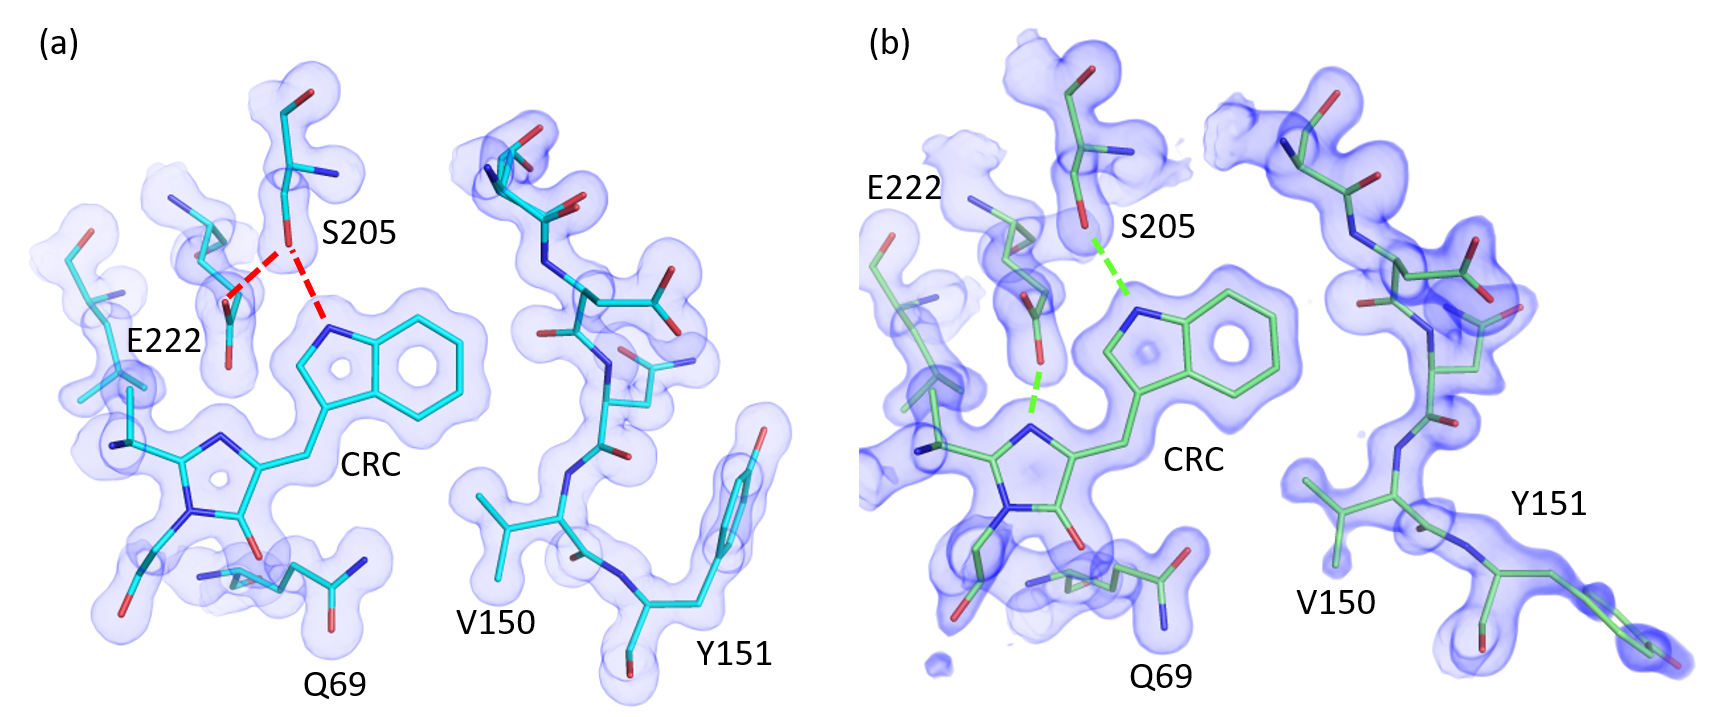
\includegraphics[width=\textwidth]{images/T-Cer/T-Cer_pH8vs4.png}
    \hfill
    \caption{Characterisation of T-Cer crystallised at pH 8: (a) Overview of the chromophore (CRC) environment in a structure of T-Cer at neutral pH (1.2 \AA\  resolution, 2\(F_{obs} - F_{calc}\) electron density map contoured at 1.0 \textsigma\ level) collected on beamline ID30b, at the ESRF, red dashed lines represent H-bonds. The chromophore adopts the Z,Z configuration, the carboxyl head of E222 is H-bonded to the hydroxyl group of S205. That same hydroxyl is H-bonded to the indole ring of the chromophore. (b) In the first structure of T-Cer solved from a crystal grown at pH 4.0, 2D (1.2 \AA\ resolution), the configuration Z,Z (lime) is fully populated, S205 is H-bonded to the chromophore, but E222 is no longer H-bonded to S205. The electron density on V150 and Y151 is not as well-defined as for nearby amino acids.}
    \label{fig:T-Cer_pH8vs4}
\end{figure}
\subsection{The structure of T-Cer at acidic pH reveals a metastable Z,Z configured chromophore}
Then, to produce an end-state structure, T-Cer was crystallised at pH 4.0 (conditions in Section \ref{sec:mat_cryst}). Here, we expected a high-resolution structure containing the chromophore in the configuration E,Z. Instead, the chromophore in the first structure of T-Cer solved from a crystal grown at acidic pH was in the Z,Z configuration (Table \ref{tab:structure-list}, Fig. \ref{fig:T-Cer_pH8vs4} (b)). 

\vspace{2mm}

The chromophore isomerisation happens over 80 ms in solution. Therefore, it is reasonable to assume that the chromophore of T-Cer would have isomerised into the configuration E,Z almost instantly when the protein sample was mixed with the pH 4.0 mother liquor, and certainly before crystallisation could happen. And yet, the carboxylic head of E222 is rotated by 20 \degree in the pH 4.0 structure, compared to its position in the REF structure, its H-bond with S205 is severed and it is now H-bonded to the N2 atom of the imidazolinone ring of the chromophore instead (Fig. \ref{fig:T-Cer_pH8vs4} (b)). This reconfiguration of the H-bond network reveals that E222 is indeed protonated in the acidic pH structure. 
This project was founded under the hypothesis that the chromophore adopted the configuration Z,Z at physiological pH, and switched to E,Z at acidic pH in 80 ms. Being able to observe a stable chromophore in the Z,Z configuration at pH 4.0 contradicted one of our hypotheses, as it suggested that the configuration of the chromophore was not (only) pH-dependent. 

\subsection{Crystals of T-Cer cryo-cooled at different delays after they appeared reveal a slow build-up of the E,Z configuration over weeks}

The first structure of T-Cer at pH 4.0 was solved from a crystal cryo-cooled two days after it had grown (overnight). Crystals were fished from the same plate several times to reproduce these results. As a result, the structures of T-Cer at pH 4.0 came from crystals cryo-cooled 8, 15 and 30 days after they had grown, the resulting crystal structures are named \(n\)D where \(n\) is the number of days separating crystal growth (usually overnight) and crystal cryo-cooling (trapping the species contained in the crystal at that time). Accordingly, the first structure (represented in Fig. \ref{fig:T-Cer_pH8vs4} (b)) will be referred to as structure 2D. 

To our surprise, structures 15D and 30D contained a mixture of both configuration and the configuration E,Z exclusively, respectively (Fig. \ref{fig:T-Cer_pH8vs4} (b) and (c)). It appeared that the fraction of E,Z configured chromophore was building up in the crystals as they were left in their crystallisation drop (aged).  

\vspace{2mm}

In 8D, the thinning electron density on V150 suggests it has become flexible (Fig. \ref{fig:ageing_struc} (a)). The spike of electron density under the indole ring of the chromophore suggests that a low occupancy population of the E,Z configuration has appeared. Additionally, the electron density around the imidazolinone ring  has broadened, indicating the coexistence of many alternatively confirmed species that cannot be modelled. Accordingly, E222 is further tilted towards the imidazolinone ring, presumably following its movement.

In 15D, a 55/45 mix of configurations Z,Z (green) and E,Z (purple) and their respective networks of alternate conformations can be observed (Fig. \ref{fig:ageing_struc} (b)). In the E,Z configuration, the imidazolinone ring  retreats into the chromophore pocket, presumably to give the indole head of the chromophore some space to isomerise. There is no electron density (or negligible amounts) between the reference and translated conformations of V150. 


It appears that the slow transition of the 7th strand over days/month that controls the isomerisation \textit{in crystallo} as in structure 30D, the chromophore is entirely E,Z configured and the 7\textsuperscript{th} strand is now stable, in its 'opened' position. Q69 has adopted a new configuration, and a stable water molecule stabilises the indole ring of the chromophore (Fig. \ref{fig:ageing_struc} (c)). Upon closer inspection, the position of V150 in structure 2D would clash with the E,Z configuration of the chromophore. In structure 30D, V150 is translated a full 1 Å outward of the chromophore pocket. Nearby amino acids of the 7\textsuperscript{th} strand are also translated outward, to a lesser degree. 
\begin{figure}[H] %bt!]
    \centering
        \noindent 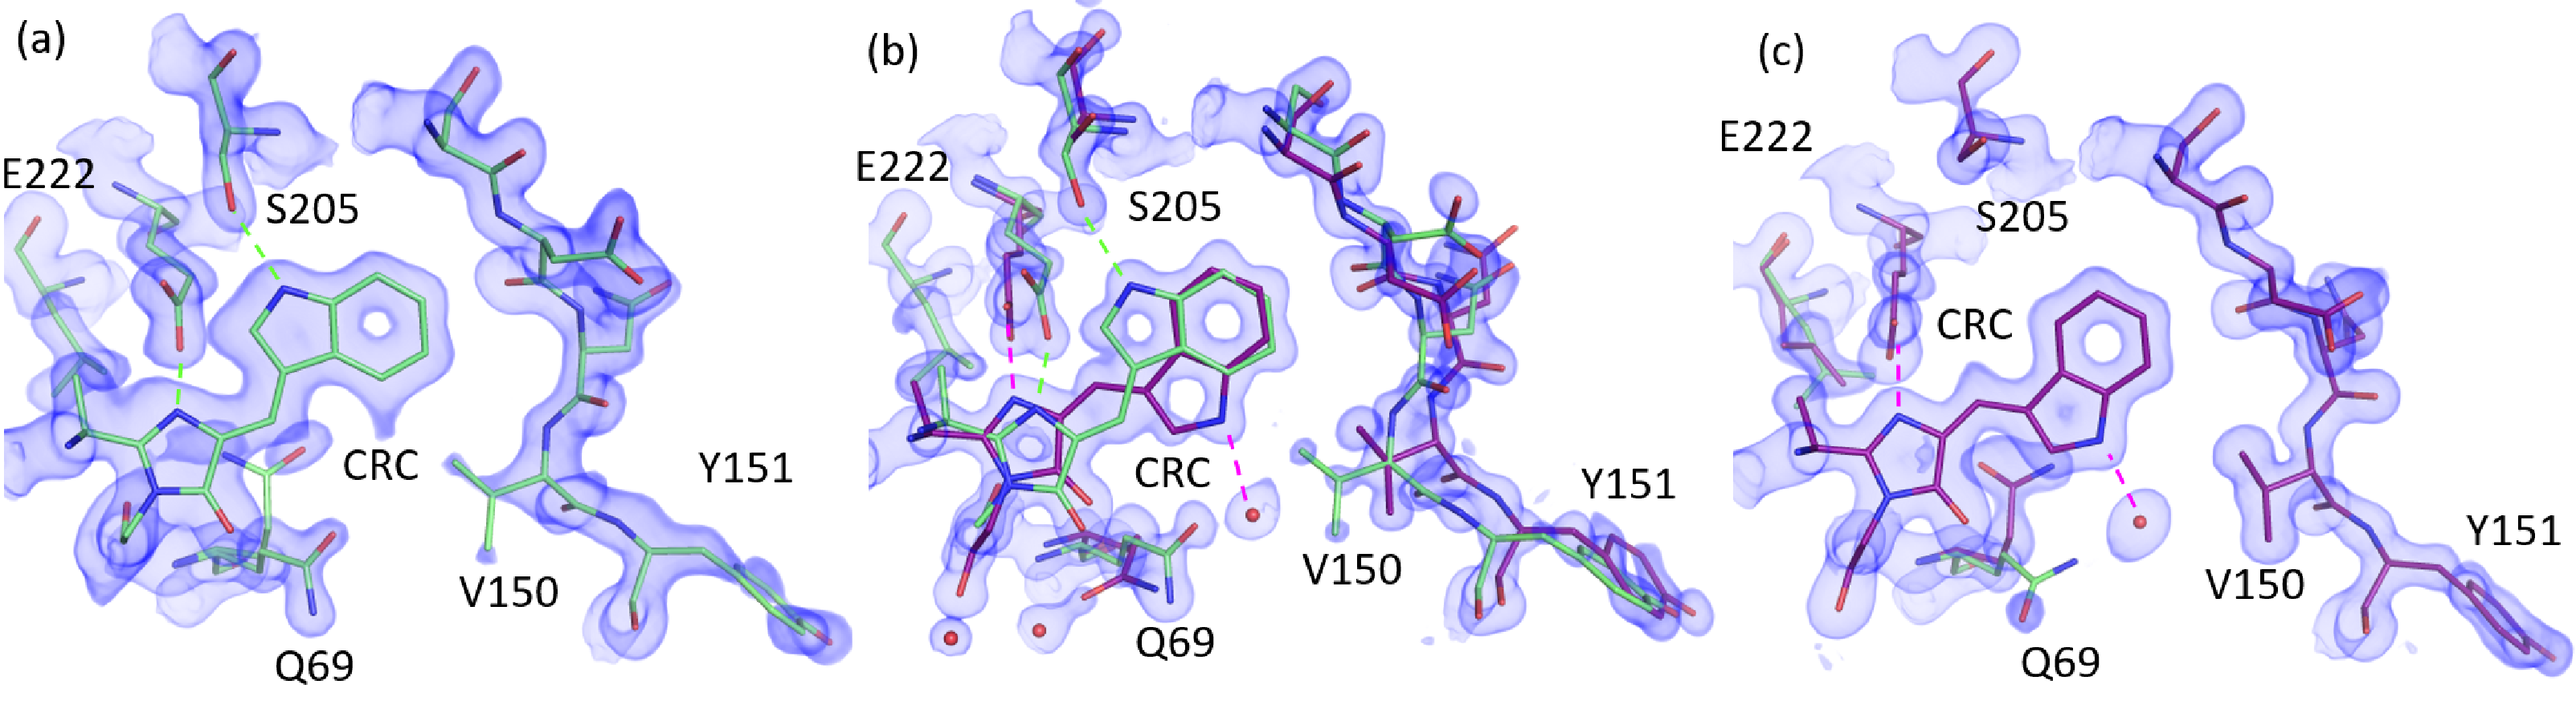
\includegraphics[width=\textwidth]{images/T-Cer/ageing_struc.pdf}
    \hfill
    \caption{Ageing of T-Cer crystals grown at pH 4.0 evidenced via structures of T-Cer cryo-cooled at increasing delays after the crystals appeared. 2\(F_{obs} - F_{calc}\) electron density map contoured at 1.0 r.m.s.d, overlaid on the refined models for the Z,Z conformed (green) and E,Z conformed (purple) species present in the crystal. Dashed lines (green or magenta) represent H-bond networks of both species (respectively Z,Z and E,Z conformed) (a) In 8D (1.4 \AA\ resolution), hint of electron density supporting the low occupancy presence of the configuration E,Z can be seen on the chromophore. The chromophore remains mostly in the Z,Z configuration. S205 and E222 are still engaged in the same H-bond network as in 2D. The electron density on V150 has thinned. (b) In 15D (1.1 \AA\ resolution), both the Z,Z and E,Z configurations can be observed for the chromophore, as well as alternate conformations for S205 and E222, and the 7\textsuperscript{th} strand, one is similar to the conformation in 2D (lime, Z,Z configuration, 55 \% occupancy) and one corresponds to the E,Z configuration (purple, 45 \%). In the latter species, the chromophore is supported by a novel H-bond network, where S205 is disengaged and points upwards, E222 is still H-bonded to the N2 atom of the imidazolinone ring, but has rotated 180 \degree. In addition, the region of the 7\textsuperscript{th} strand is pushed back to allow the E,Z configuration of the chromophore to exist, with V150 being translated of a full 1 \AA. Finally, a novel stable water position, H-bonded to the indole ring of the chromophore, occupies the space freed by the retreat of Q69. (c) The chromophore in 30D (1.4 \AA\ resolution) is fully converted, with only the E,Z configuration of the chromophore and its corresponding alternate conformation network (purple) remaining.}
    \label{fig:ageing_struc}
\end{figure}

The study of the build-up of the E,Z configuration over time (dubbed the 'ageing phenomenon') yielded several insights, altering our working hypothesis that the chromophore adopts the Z,Z configuration at physiological pH, and E,Z configuration at low pH. 
\begin{enumerate}
    \item T-Cer crystallises with its chromophore in the Z,Z configuration. 
    \item At acidic pH \textit{in crystallo}, a metastable (\textasciitilde 2 weeks of half-life) species of T-Cer whose chromophore is in the Z,Z configuration (species MZZ, best represented by structure 2D) initially exists.
    \item MZZ can exist because of a slow reorganisation of the chromophore pocket, involving the 7\textsuperscript{th} strand of the \textbeta-barrel. 
\end{enumerate}

This casts doubts on the configuration of the chromophore in the species formed in 80 ms in solution: does the observed blue-shift correspond to a switch from configuration Z,Z to configuration E,Z, or is the chromophore of T-Cer still in the configuration Z,Z at the end of the experiment? 



\subsection{Matching the X-ray structures of T-Cer to spectroscopic intermediates with UV-vis absorption spectroscopy in solution and \textit{in crystallo}.}
In order to answer that question, we needed to bridge the gap between the species present at the end in-solution time-resolved experiment and our structures of ageing T-Cer. First, we needed to characterise the UV-vis absorption spectroscopy signature of T-Cer over pH in a non-time-resolved manner. 
\subsubsection{The UV-vis absorption spectroscopy signature of T-Cer in solution over pH}
Absorption spectra of T-Cer in solution were recorded from pH 8.0 (blue) to 3.0 (red) Fig. \ref{fig:T-Cer_insolution_pH_static}. From pH 8.0 (blue) to 5.5 (yellow-green), the main absorption band of T-Cer's chromophore loses its two-peak structure, and the centre of mass of the peak blue shifts from 438 nm to 436 nm, as in the time-resolved absorption spectroscopy experiment (Fig. \ref{fig:pH_TRspectroinsolution} (b)). The starkest change occurs between pH 5.5 (yellow-green) and 5.0 (orange), where the main absorption band's centre of mass is significantly blue-shifted to 427 nm (an 11 nm shift from that of the reference state). It further blue-shifts to 423 nm at pH 3.5. Then, at pH 3.0, the centre of mass of the peak reaches 410 nm, probably after the chromophore is exposed to the solvent upon acid-induced denaturation of the protein.
\begin{figure}[H] %bt!]
    \centering
        \noindent 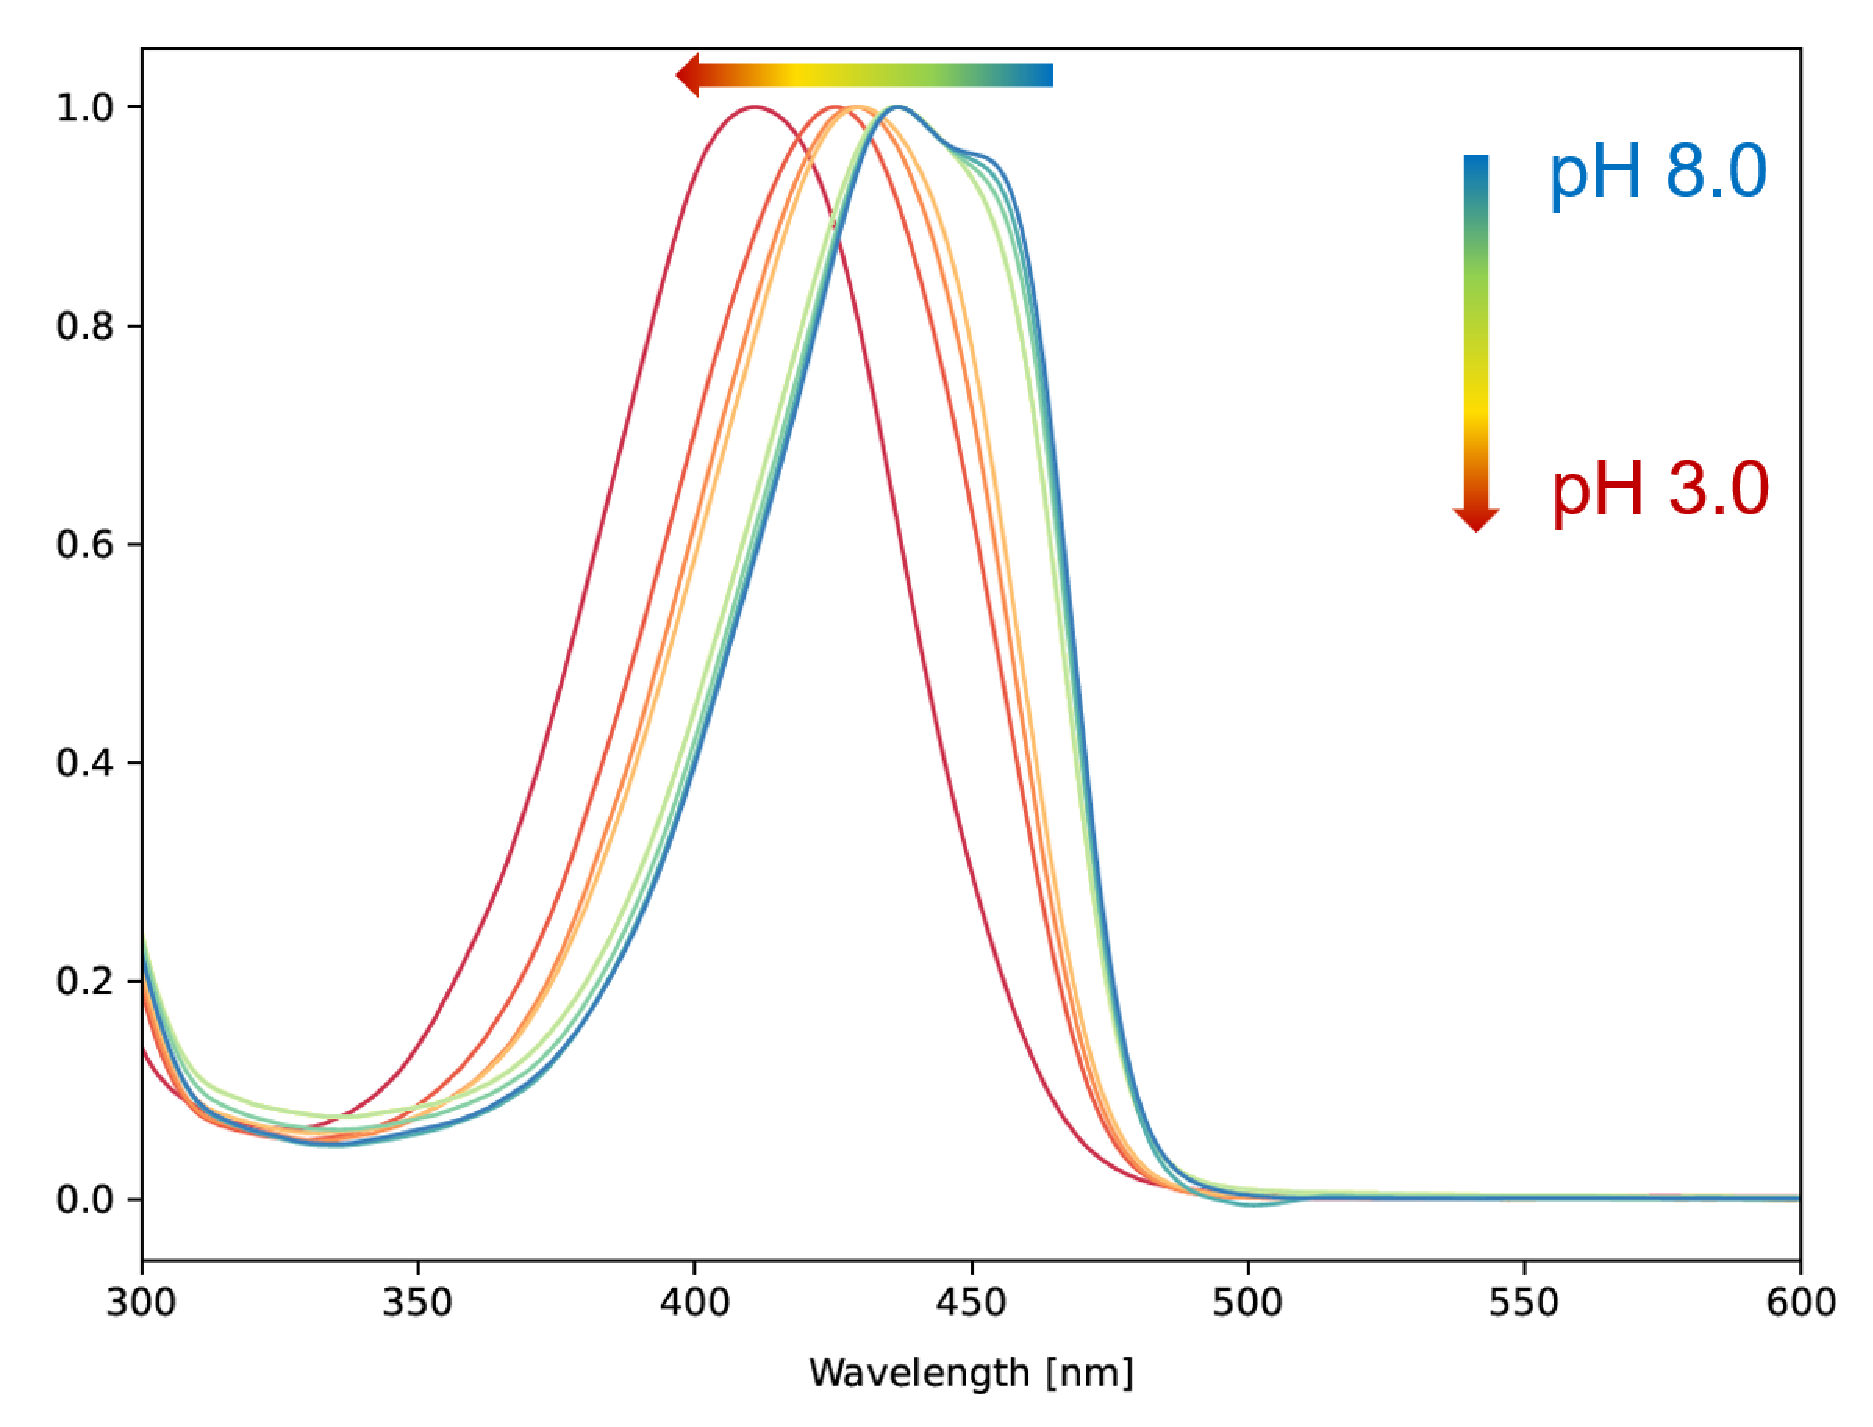
\includegraphics[width=0.6\textwidth]{images/T-Cer/In_solution_static_T-Cer.pdf}
    \hfill
    \caption{absorption spectra of T-Cer in solution from pH 8.0 (blue) to 3.0 (red). At neutral pH, the absorption spectroscopy spectrum features a main absorbance peak centred around 435 nm and a shoulder around 450 nm. From pH 8.0 to 6.0, this shoulder is progressively lost. From pH 6.5 to 5, the main absorption band blue-shifts to 430 nm. From pH 5 to pH 4, the main absorption band blue-shifts further to 425 nm.}
    \label{fig:T-Cer_insolution_pH_static}
\end{figure}

\subsubsection{The evolution of the \textit{ic}AS spectrum of T-Cer crystals as they 'age'}
Then, \textit{ic}AS spectra were recorded on crystals cryo-cooled at several points during the 'ageing' process to potentially match their spectroscopic signature with those of the time-resolved pH drop spectroscopy experiment and steady pH points. The spectra are named s\(n\)D accordingly.

In s1D (coloured red, Fig. \ref{fig:ageing_spec}) have a wide absorption band centred on 425 nm, with shoulders at 420, 438 and 450 nm  This most likely corresponds to a mix of species, which probably includes the reference stable Z,Z chromophore (responsible for the 438 and 460 nm shoulders). 

In s2D (coloured orange in Fig. \ref{fig:ageing_spec}), the shoulders at 438 nm and 460 nm disappear, blue-shifting the centre of mass to 420 nm. In s3D:s5D (respectively coloured yellow and light-orange in Fig. \ref{fig:ageing_spec}), the shoulder at 410 nm grows, resulting in a further blue shift of the centre of mass of the absorption band. In s9D:s11D (coloured green to teal in Fig. \ref{fig:ageing_spec}), the shoulder at 410 nm disappears, and the entire band red-shifts to 425 nm. Finally, in s15D (coloured blue spectrum in Fig. \ref{fig:ageing_spec}), the centre of mass of the absorption band is further red-shifted to 430 nm, with a shoulder at 460 nm. 

The 410:420 nm species observed for s2D:s5D, corresponding to MZZ, do not match the last spectrum measured 80 ms after the mixing-induced pH drop during the time-resolved spectroscopy experiment in solution, whose absorption is maximal at 438 nm. Neither do they match the UV-vis spectra of T-Cer in solution at pH 4.0, whose absorption band is maximal at 430 nm. s15D much better matches the spectrum of T-Cer in solution at pH 4.0. However, a shoulder at 460 nm, absent in solution, remains in the spectrum of the 15D crystal, perhaps because it contains a mix of configurations Z,Z and E,Z. \textbf{We can retain the hypothesis that the species formed at pH 4.0 in solution exhibits a chromophore in the E,Z configuration.}

\begin{figure}[H] %bt!]
    \centering
        \noindent 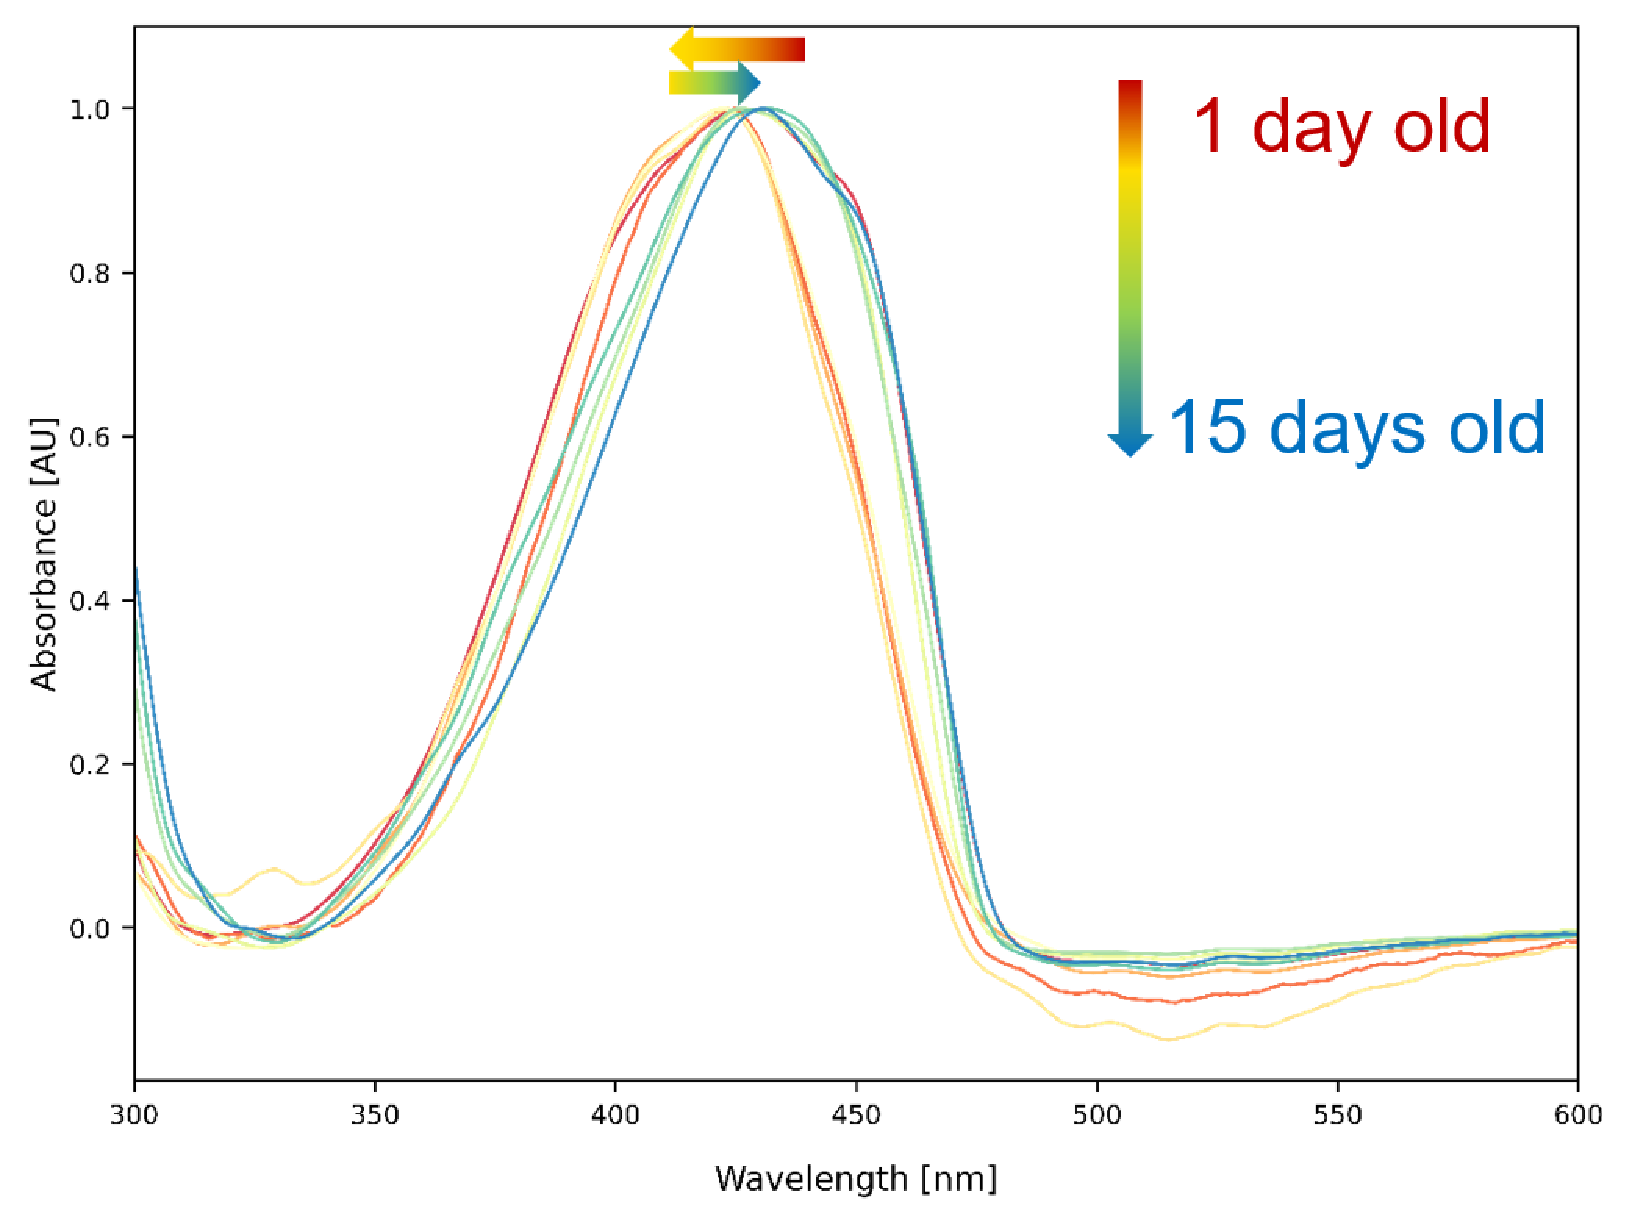
\includegraphics[width=0.7\textwidth]{images/T-Cer/ageing_spectra.pdf}
    \hfill
    \caption{\textit{in crystallo} absorption spectra of T-Cer crystals at pH4 over time. In a 1D crystal (red curve), the main absorption band of the spectrum is wide, with a main peak at 425 nm, and shoulders at 420, 425, 435 and 450 nm. In a 2D crystal (orange curve), the main peak of the absorption band is now at 425 nm. In a 3D, 4D and 5D crystal (light orange to bright yellow curves), the main absorbance peak is at 425 nm, and the shoulder at 420 nm has increased in relative height. In 9D and 13D crystals (faded yellow and green curves), the absorption band features only one wide peak centred at 430 nm. After two weeks (blue curve), the absorption band features a main peak at 430 nm and a small shoulder at 450 nm.}
    \label{fig:ageing_spec}
\end{figure}

It appears that the crystalline artefact is not the existence of the E,Z configuration, but rather a prohibited movement of the 7\textsuperscript{th} strand, allowing MZZ to exist, and which exhibits a significantly more blue-shifted absorption band. Several hypotheses, including decreased hydration and mechanical hindrance by the presence of crystal packing points and very close monomers, can explain this prohibited dynamics \textit{in crystallo} (discussed in Section \ref{sec:packingartefact}). The rigidity of the 7\textsuperscript{th} strand is particularly unexpected because this strand is dynamic in Cerulean \parencite{lelimousinIntrinsicDynamicsECFP2009}.

Nevertheless, the sequence of structural reconfiguration leading up to the appearance of configuration E,Z during the 'ageing phenomenon' can serve as a putative model for the sequence of events occurring during the switch from configuration Z,Z to E,Z after a pH drop.

Of note, the lattice parameters in \(n\)D are noticeably shrunk compared to that of REF. This is most pronounced for the C-axis of the unit cell, which is 5 \AA\ shorter in \(n\)D Table \ref{tab:structure-list}. 

\subsection{Atomic resolution structures of T-Cer reveal a different conformation of the C-terminus at physiological and acidic pH}

As for the 'mechanical hindrance' hypothesis, the C-terminal \textalpha-helix of T-Cer (non-visible in published structures of Cerulean \parencite{maloXrayStructureCerulean2007, gotthardCapturingBluelightActivated2023}) is conformed differently REF (green) and \(n\)D (cyan) (Fig. \ref{fig:T_Cer_cter}). In \(n\)D (cyan in Fig. \ref{fig:T_Cer_cter}), the c-terminal \textalpha-helix is positioned near Y200 and Y151, two amino acids which are required to move during the translation of the 7\textsuperscript{th} strand (zoomed-in red rectangle in Fig. \ref{fig:T_Cer_cter}). The additional bulk of the helix could prevent the movement of the 7\textsuperscript{th} strand and thereby prohibit chromophore isomerization. In REF, the C-terminus is positioned away from the \textbeta-barrel. 

\vspace{2mm}

Therefore, T-Cer might be more flexible \textit{in crystallo} when the crystals are grown at pH 8.0. We tried to verify this hypothesis by soaking T-Cer crystals grown at pH 8.0 into pH 4.0 mother liquor, but they did not survive the soak. 

\begin{figure}[H] %bt!]
    \centering
        \noindent 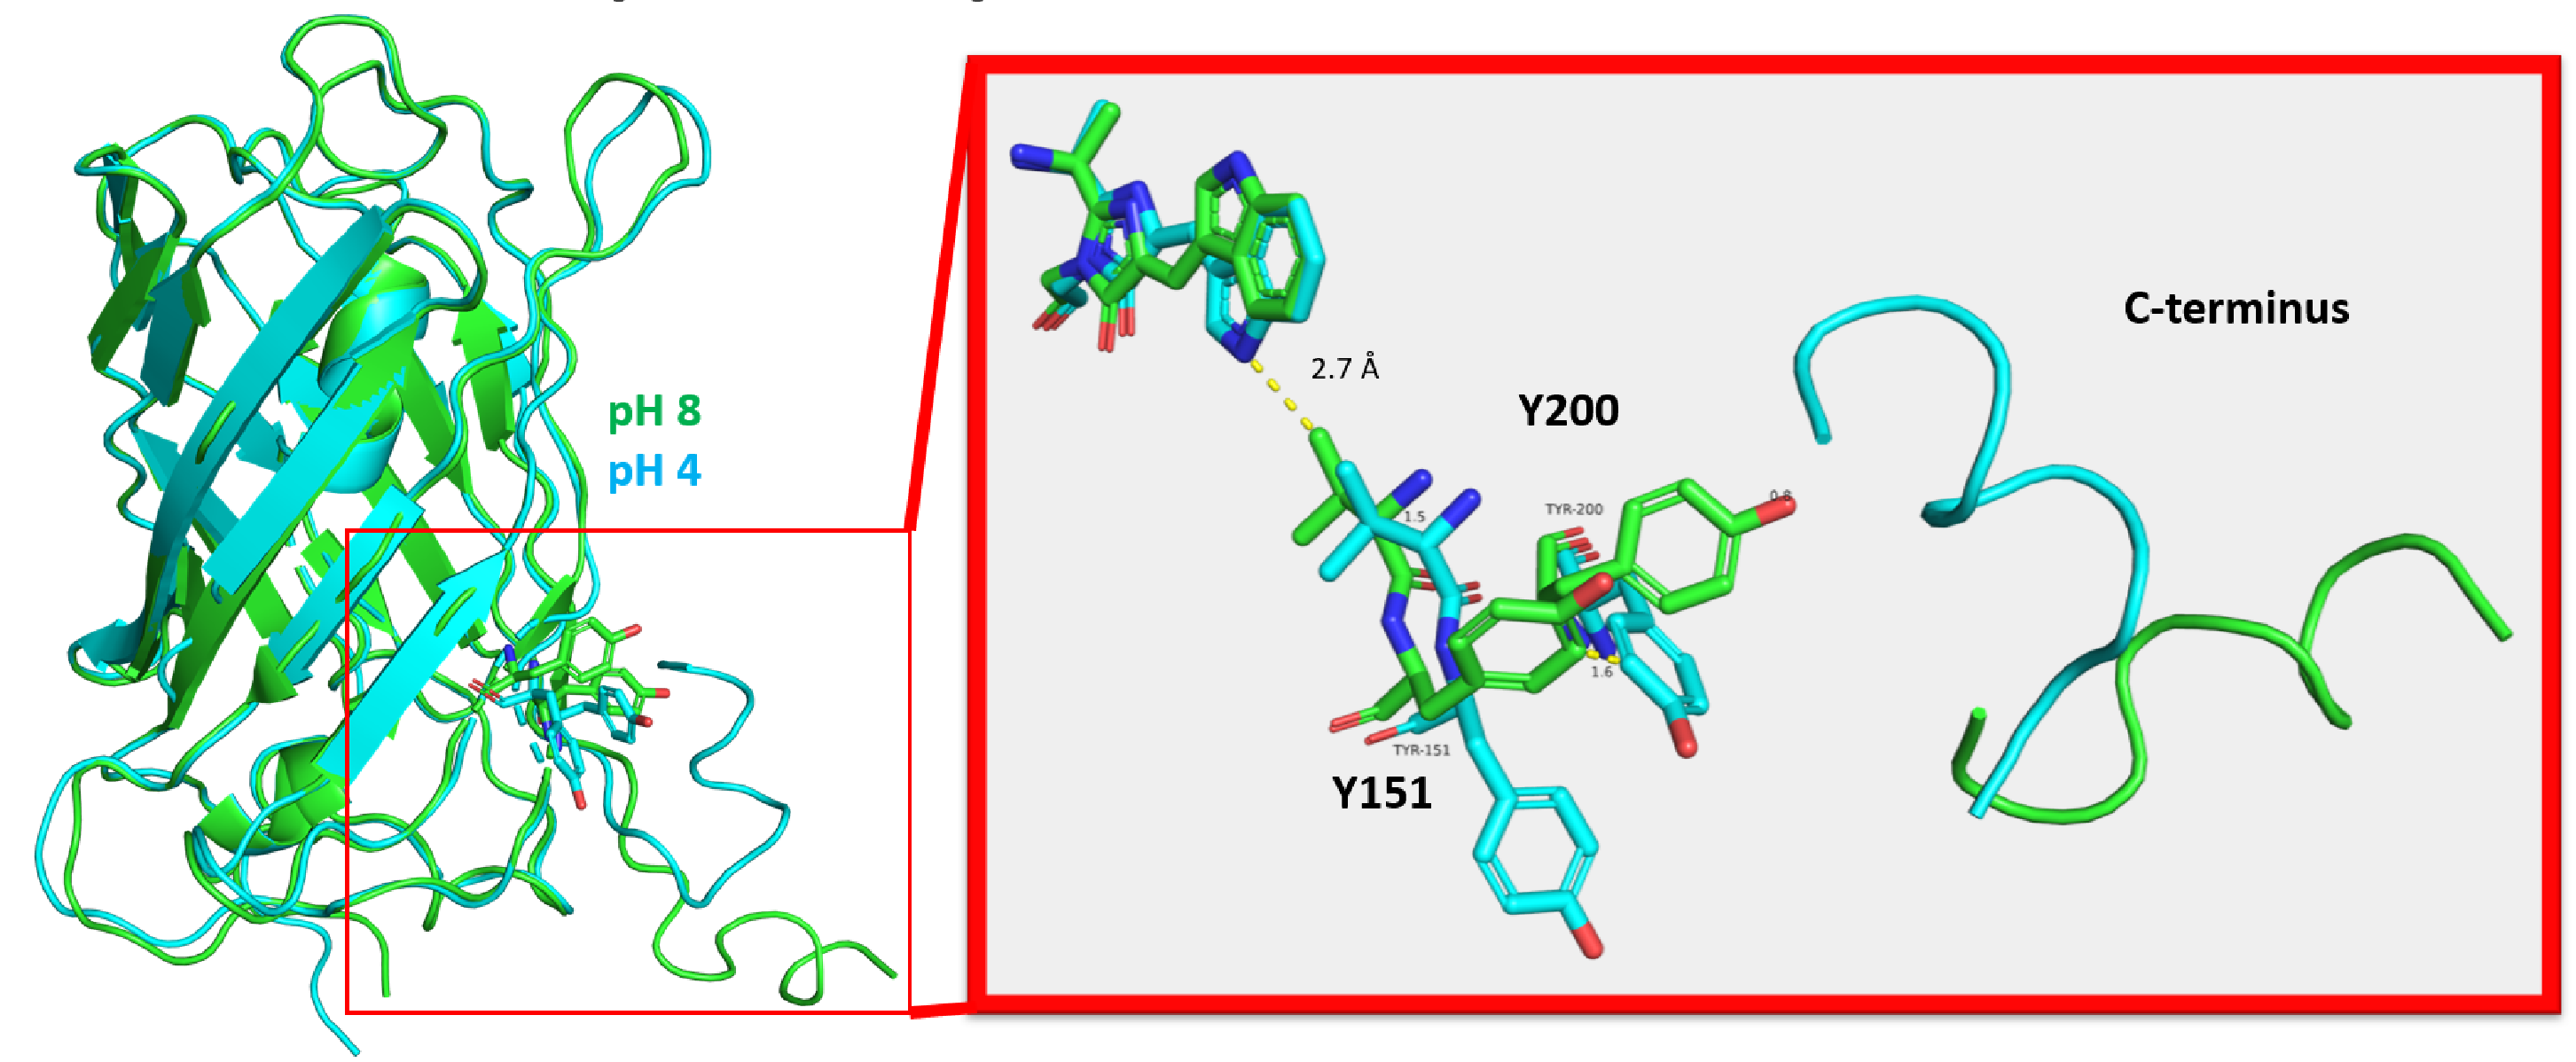
\includegraphics[width=\textwidth]{images/T-Cer/C-ter_T-Cer.pdf}
    \hfill
    \caption{Comparison of REF (blue) and 2D (green) structures revealing a different conformation of the C-terminus of T-Cer at acidic and neutral pH, which govern the dynamics of the 7th \textbeta sheet of T-Cer. In crystals obtained at neutral pH, the helix is angled at approximately 90 \degree from the \textbeta-barrel of the chromophore. In crystals obtained at pH 4.0, the helix is positioned along the \textbeta-barrel, close to the 7\textsuperscript{th} strand of the barrel. The tip of the helix in 2D comes close to the position of Y200 and Y151. This hinders the flip of Y200 and Y151, which occurs concurrently with the change of conformation of V150.}
    \label{fig:T_Cer_cter}
\end{figure}

\textbf{To assess whether the chromophore of crystals grown at pH 8.0 would switch from configuration Z,Z to configuration E,Z when the pH in the crystal was lowered, we performed a series of TR-SSX experiments, where the state of T-Cer micro-crystals was probed at various delays after they had been mixed with an acidic solution. }

\section{TR-SSX appraisal of the reaction of T-Cer to a mixing-induced pH drop}

The first TR-SSX experiment took place remotely (due to the COVID-19 health crisis) at beamline P11. Microcrystals of T-Cer were produced by the P11, in DESY team using the protocol described in Section \ref{sec:microcrystallisation}, and mixed with a pH 4.0 mother liquor solution using the CFEL tape-drive \parencite{beyerleinMixanddiffuseSerialSynchrotron2017, zielinskiRapidEfficientRoomtemperature2022} (scheme and setup described in Section \ref{sec:presenting_tpd_P11}). 

\subsection{First tape-drive experiment at P11}

Datasets were recorded 67 to 760 ms after mixing (Table \ref{tab:structure-list}) to sample the time regime defined by the time-resolved UV-vis spectroscopy experiment in solution (Section \ref{sec:prior_T-Cer}). Unfortunately, no meaningful difference between reference and time-points could be observed in the electron density, neither by calculating an \(F_{obs}(time\ point) - F_{obs}(reference\mbox{-}state)\) difference map nor by refining the datasets (reference of the experiment (REF-TPD-1 and 760 ms time-point 760MS-P11 are represented in Fig. \ref{fig:tpd1}). Of note the crystalline lattice of REF-TPD-1 is slightly expanded (1 \AA\ on the C-axis, Table \ref{tab:structure-list}) compared to that of REF, which is expected between datasets collected at room temperature (220K) and cryogenic temperature (100K). 

\vspace{2mm}

Several improvements of the experimental scheme were made for the following beamtimes. T-Cer was submitted to limited proteolysis to increase its flexibility \textit{in crystallo} (Section \ref{sec:limited_proteolysis}). Crystals were mixed with 1M pH 4.0 buffer instead of pH 4.0 mother liquor to decrease viscosity and produce an excess of protons after mixing. 

\subsection{Fixed-target LAMA experiment at P14-2 TREXX}\label{sec:T-REXX}

Using the fixed target liquid dispensing setup described in Section \ref{sec:LAMA}, a datasset was recorded three seconds after the microcrystals of T-Cer were shot by a droplet of pH 4.0 sodium acetate (3S-LAMA, \ref{tab:structure-list}), as well as a reference (REF-LAMA).

In 3S-LAMA, the head of E222 is rotated 30 \degree clockwise, also away from the indole ring of the chromophore and H-bonded to the imidazolinone ring  and S205 is tilted towards E222, away from the indole ring of the chromophore (both are coloured in purple in Fig. \ref{fig:T-Cer_TREXX_results} (b)). Additionally, the electron density is lost on the side-chain of Y151. However, the chromophore and the rest of the chromophore pocket are identical (or comparable) in REF-LAMA and 3S-LAMA (Fig. \ref{fig:T-Cer_TREXX_results} (c)). 

\vspace{2mm}

The 3S-LAMA contains the structure of MZZ, where E222 is protonated, but the chromophore is still in the Z,Z configuration because the 7\textsuperscript{th} strand has not moved yet.
\begin{figure}[H] %bt!]
    \centering
        \noindent 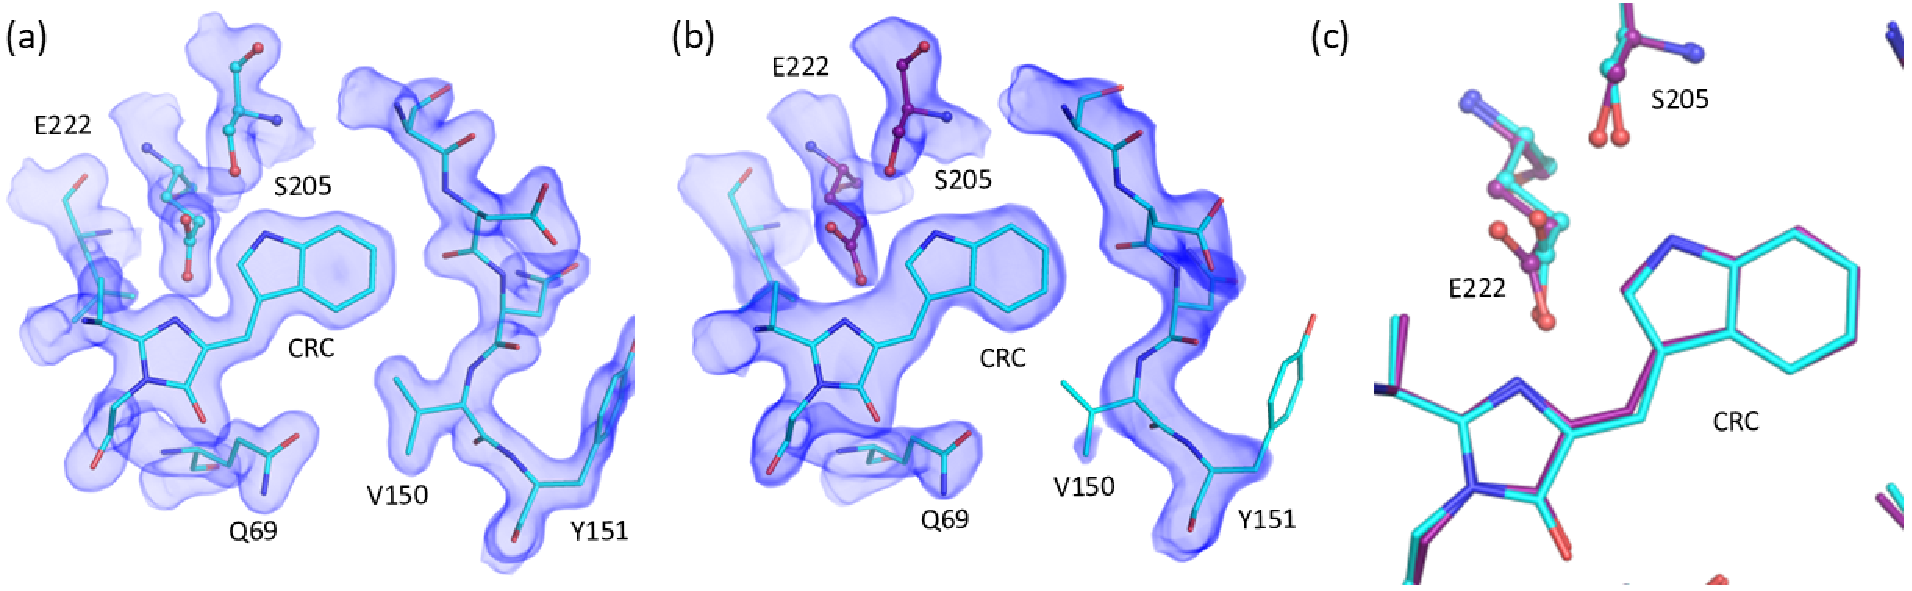
\includegraphics[width=\textwidth]{images/T-Cer/TREXX_results.pdf}
    \hfill
    \caption{Results of the T-REXX beamtimes : \(2F_{obs} - F_{calc}\) electron density map contoured at 1.5 \textsigma\ level (a) REF-LAMA (1.7 \AA\ resolution) features a well-defined V150, Y151 as well as an engaged S205 and E222, and Z,Z chromophore. (b) 3S-LAMA (2.3 \AA\ resolution) where Y151 and V150 have flexible side-chains. S205 is tilted upwards, and E222 is disengaged (30 \degree clockwise rotation). These signs suggest that the pH drop has occurred, but the isomerization has not. (c) Superposition of the atomic models of REF-LAMA (cyan) and 3S-LAMA (purple) revealing the difference in orientation of S205 and E222.}\label{fig:T-Cer_TREXX_results}
\end{figure}

\subsection{Second tape-drive mixing experiment at P11}\label{sec:P11-2}

Microcrystals were mixed with 1M pH 4.0 buffer using the fast mixing nozzle of the CFEL tape drive (setup described in Section \ref{sec:presenting_tpd_P11}). Both sodium acetate (Section \ref{sec:acetate}) and sodium citrate (Section \ref{sec:citrate}) were trialled. 

\subsubsection{Sodium acetate}\label{sec:acetate}
Time points were recorded 3 s (3S-TPD-Ac) and 8 s (8S-TPD-Ac) after the crystals were mixed with sodium acetate to validate the reproducibility of the results obtained at T-REXX and further explore the timeline. The reference state of this experiment, REF-TPD, is equivalent to REF-LAMA.

3S-TPD-Ac closely resembles 3S-LAMA (rotated carboxylic head of E222 and tilt of S205, (Fig. \ref{fig:T-Cer_P11-2_Ac_results} (b)). In 8S-TPD-Ac, V150 becomes slightly dynamic (Fig. \ref{fig:T-Cer_P11-2_Ac_results} (c)), but S205 seems to have returned to its initial position (only the model of 3S-TPD-Ac, coloured purple, differs from REF-TPD in Fig. \ref{fig:T-Cer_P11-2_Ac_results} (d)). It is clear that both 3S-TPD-Ac and 8S-TPD-Ac match the structure of MZZ. 
\begin{figure}[H] %bt!]
    \centering
        \noindent \includegraphics[width=\textwidth]{images/T-Cer/T-Cer_tpd_P11-2_acetate.pdf}
    \hfill
    \caption{Structures of T-Cer after a pH drop induced by mixing with Sodium acetate, 2\(F_{obs} - F_{calc}\) electron density maps contoured at 1.0 \textsigma\ level (a) REF-TPD (2.0 \AA\ resolution) featuring a well-defined V150, Y151 as well as an engaged S205 and E222, and Z,Z chromophore. (b) 3S-TPD-Ac (1.9 \AA\ resolution) S205 (purple) is tilted away from the chromophore. E222 exists in two conformations (green and purple), which are both rotated away from the chromophore. The electron density on Y151 is less defined.  (c) 8S-TPD-Ac (2.2 \AA\ resolution) S205 is back to its initial conformation (coloured in cyan). E222 is fully rotated away from the chromophore (coloured in purple). V150 and Y151 have lost stability. (d) Superposition of refined models for REF-TPD (cyan), 3S-TPD-Ac (purple) and 8S-TPD-Ac (blue), showing the progressive rotation of E222 away from the chromophore and the tilt of S205 at 3s. V150 and nearby amino acids are backing away from the chromophore.: }\label{fig:T-Cer_P11-2_Ac_results}
\end{figure}


\subsubsection{Sodium citrate}\label{sec:citrate}
Time points were recorded 300 ms (300MS-TPD-Ci) and 1 s (1S-TPD-Ci) after mixing  as comparison points with the results of the first beamtime (Supplementary section \ref{sec:P11-1}).  Time points recorded 3 s (3S-TPD-Ci) and 8 s (8S-TPD-Ci) after the crystals were mixed with sodium citrate to serve as comparison points were found to be identical to 3S-TPD-Ac and 8S-TPD-Ac. A last time-point was recorded 16 s after mixing (16S-TPD-Ci) to sample the long-term dynamics of the chromophore. 

In 300MS-TPD-Ci, E222 exists in two conformations (Fig. \ref{fig:T-Cer_P11-2_Ci_results} (a)), which are both rotated away from S205. One is H-bonded to the imidazolinone ring  of the chromophore (MZZ-like, purple) and one is H-bonded to a stable water molecule (not represented) positioned in the background of Fig. \ref{fig:T-Cer_P11-2_Ci_results} (a) (cyan). From 1S-TPD-Ci to 16S-TPD-Ci (Fig. \ref{fig:T-Cer_P11-2_Ci_results} (b) and (c)), only the MZZ-like conformation of E222 remains. 
\begin{figure}[H] %bt!]
    \centering
        \noindent \includegraphics[width=\textwidth]{images/T-Cer/T-Cer_tpd_P11-2_citrate.pdf}
    \hfill
    \caption{Structures of T-Cer after a pH drop induced by mixing with Sodium citrate. All 2\(F_{obs} - F_{calc}\) electron density maps are contoured at 1.0 \textsigma\ level (a) In 300MS-TPD-Ci (1.9 \AA\ resolution), E222 exists in two conformations, which are both rotated away from the chromophore. The electronic density on V150 is still well-defined, but that of Y151 is slightly less defined.  (b) In 1S-TPD-Ci (1.9 \AA\ resolution), E222 is fully rotated away from the chromophore. The side chains of V150 and Y 151 are only partially covered by electron density. (c)  In 16S-TPD-Ci (2.1 \AA\ resolution), E222 is fully rotated away from the chromophore. The side chains of V150 and Y 151 are well covered by electron density, but their strand has moved 0.1 \AA\ away from the chromophore.}\label{fig:T-Cer_P11-2_Ci_results}
\end{figure}

\subsubsection{Discussion of the results produced in TR-SSX beamtimes}\label{sec:discussion_P11_2}

While it has not fully stabilised in the MZZ-like conformation yet, E222 is likely protonated in 300MS-TPD-Ci (Fig. \ref{fig:T-Cer_P11-2_Ci_results} (a)). In comparison, the H-bond between S205 and E222 is intact in 760MS-TPD-1 (Supplementary figure \ref{fig:tpd1} (b)).  Consequences of a pH drop could be observed this time in the ms time-domain, while it they could not in the first beamtime. \textbf{The limited proteolysis step and use of 1M pH buffer succeeded in increasing the flexibility of T-Cer \textit{in crystallo} and/or decreasing the diffusion time of protons in the crystal.}

\vspace{2mm}

Thanks to these advances, the diffusion of protons in the crystals occurs on almost the same time scale as the configuration switch in solution, which would make a TR-SSX able to monitor the mechanism of transition from configuration Z,Z to E,Z after a pH drop. However, despite this advance, all datasets recorded past 300 ms contain a species akin to MZZ, whose chromophore is still in the Z,Z configuration. A trend corresponding to a slight outward translation of V150 (0.1 \AA\ at most) over time can be sighted when modelled from the recorded time points (Fig. \ref{fig:T-Cer_P11-2_Ac_results}), but the system seems stuck in the MZZ state, blocked by the rigidity of the 7\textsuperscript{th} strand.

We can therefore answer some of the questions raised previously. Even in crystals of T-Cer grown at pH 8.0, the packing of T-Cer crystals is clearly inhibiting the movements of the 7\textsuperscript{th} strand, which are needed for the configuration switch. We cannot discern the mechanism underlying the fast switch from configuration Z,Z to E,Z with TR-MX, because even if the isomerisation was to occur \textit{in crystallo}, we could only observe metastable species, and not the reaction intermediate leading from one to another. Finally, our best model so far for this transition is the sequence of events occurring during the ageing phenomenon, which allowed us to observe some of these metastable species. 

Nevertheless, the early response of T-Cer \textit{in crystallo} to a pH drop is now characterised. T-Cer can serve as a commissioning tool for mixing-based TR-SSX setups. 

\section{Commissioning of a Tape-drive setup on ID29}\label{sec:ID29}

In September 2022, beamline ID29 (described in Section \ref{sec:presenting_ID29} was commissioned. During the first beamtime involving external users, T-Cer was used as a commissioning target for a novel tape drive setup (described in Section \ref{sec:lubeck}), as part of an ongoing collaboration with the group of Manfred Roessle in Lubeck. Microcrystals of proteolyzed T-Cer (prepared with the protocol described in Section \ref{sec:limited_proteolysis} and \ref{sec:microcrystallisation}) were mixed with 1 M pH 4.0 sodium citrate via a T-junction and exposed to the beam of ID29 60 s (60S-TPD) later. This was the first genuine TR-MX experiment of the beamline.

In 60S-TPD, E222 adopts the characteristic rotated MZZ-like conformation (Fig. \ref{fig:ID29_results} (b)), the expected reaction to a pH drop, which validates the mixing capabilities of this tape-drive setup. 

\vspace{2mm}

Additionally, S205 and Y151 appear to be dynamic (no longer covered by electron density). Finally, V150 has backed away by 0.3 \AA\ (Fig. \ref{fig:ID29_results} (c)). The movement of the 7\textsuperscript{th} strand has started in 60S-TPD: it is in a more advanced state than in 16S-TPD-Ci. This is coherent with the increased mixing-exposure delay and confirms that, \textit{in crystallo}, T-Cer keeps evolving very slowly over time after a pH drop. 
Whether the isomerisation can happen after a pH drop remains uncertain, however.
\begin{figure}[H] 
    \centering
        \noindent \includegraphics[width=\textwidth]{images/T-Cer/ID29_tape-drive_results.pdf}
    \caption{Results of the ID29 tape drive beamtime. 2\(F_{obs} - F_{calc}\) electron density map contoured at 1 r.m.s.d overlaid on key amino acids of the chromophore pocket. (a) In REF-TPD-ID29 (2.2 \AA\ resolution), the H-bond coordination of the chromophore is comparable to that of the cryogenic neutral pH structure, and all amino acids of the 7\textsuperscript{th} strand are well resolved. (b) 60S-TPD (2.4 \AA\ resolution) features the characteristic rotation of the carboxylic head of E222 (purple). In addition, the density on S205 is not well resolved, indicating that it has now become flexible. Both the side chains of V150 and Y151 have lost some of their electron density, indicating an increase in the flexibility of the 7\textsuperscript{th} strand. Finally, one side of N69 is no longer resolved, indicating that it has now become flexible. (c) superposition of the reference state (cyan) and 60s (purple) models, highlighting the rotation of E222 away from S205 as well as the movement of N69. The entire strand of the 7\textsuperscript{th} strand is coherently moving away from the chromophore (0.3 \AA\ distance between the C\textalpha of both V150). Finally, Leu 42 now exhibits an additional conformation (purple).}\label{fig:ID29_results}
\end{figure}

\section{Short T-Cer construct with enhanced flexibility enables \textit{in crystallo} chromophore isomerisation}

We identified two factors preventing the configuration switch of T-Cer's chromophore \textit{in crystallo} after a mixing-induced pH drop: the main one is the rigidity of the crystalline packing, which prevents a necessary movement of the 7\textsuperscript{th} strand, and the lesser one is the viscosity of the crystal suspension, which slows down diffusion. 

To further increase the flexibility of T-Cer \textit{in crystallo}, a construct where the C-terminus is removed (T-Cer-s) was designed (Section \ref{sec:short}). To decrease the viscosity of the crystal suspension, a new crystallisation condition and protocol were designed, where the precipitant is now NH\textsubscript{4})\textsubscript{2}SO\textsubscript{4}.  

To assess whether these innovations allow the switch of the chromophore of T-Cer-s from configuration Z,Z to E,Z \textit{in crystallo}, crystals were soaked in pH 4.0 sodium citrate. 

\subsection{Soaking T-Cer-s crystals obtained in ammonium sulfate}\label{sec:soaking}

\subsubsection{Soaking and cryo-trapping}

One such crystal, cryo-cooled after 150 s of soaking (150S-CT-S) features a negative \(F_{obs} - F_{calc}\) peak on the nitrogen atom of the indole ring of configuration Z,Z, and a twin positive peak corresponding to the position of the nitrogen atom of the indole ring in configuration E,Z configuration  (Fig. \ref{fig:T-Cer-soak-struc} (a)). 

In 150S-CT-S, a negative electron density peak on the carboxylic head of E222 indicates its departure from the REF-like conformation (Fig. \ref{fig:T-Cer-soak-struc} (a)). Additional negative peaks on the side chains of V150 and Y151, coupled with an array of positive peaks on the solvent side of the 7\textsuperscript{th} strand, indicate that it is partially 'translated'. A negative peak on the carbon of N69, coupled with a positive, two-sided density pattern above it, perfectly reflects the difference in conformation of N69 between the MZZ state and aged crystals (Fig. \ref{fig:T-Cer_pH8vs4} (b) and (d)). Positive peaks on the side of the imidazolinone ring  suggest that it moves up lightly, to allow to switch to configuration E,Z. Finally, a faint positive peak between V150 and N69 even hints at the existence of the new stable water molecule coordinating the chromophore when it is in the E,Z configuration, visible in Fig. \ref{fig:ageing_struc} (c).

\vspace{2mm}

\textbf{This is irrefutable proof that the switch from configuration Z,Z to configuration E,Z can occur \textit{in crystallo}, and validates the relevance of using the T-Cer-s construct and crystallising in  (NH\textsubscript{4})\textsubscript{2}SO\textsubscript{4}. }

Cryo-cooling crystal can favour specific conformations \parencite{fraserHiddenAlternateStructures2009,fraserAccessingProteinConformational2011}. The E,Z configuration has, so far, only been observed at cryogenic temperature; to validate its relevance, it was important to assess whether it could also be observed at room temperature. 

\subsubsection{Soaking, and collection at room temperature.}

A crystal was soaked for 60 s and mounted on the goniometer directly, protected by the flow of a humidity controller \parencite{sanchez-weatherbyImprovingDiffractionHumidity2009}, and collected after 180 s in total (180S-RT-S).

180S-RT-S showcases similar features as 150-CT-S, most notably a positive peak under the chromophore, indicating the existence of the E,Z configuration  ((Fig. \ref{fig:T-Cer-soak-struc} (b)). Features identified on E222, N69 and the full 7\textsuperscript{th} strand are also present and stronger than in 150-CT-S despite the lower resolution of 180S-RT-S.

\textbf{We can, at long last, validate that the E,Z configuration of the chromophore is induced by dropping the pH from 8.0 to 4.0 in a T-Cer-s crystal. }

Two questions are immediately prompted by this finding: (1) Is this E,Z configured species the same as that which is formed at acidic pH in solution? (2) If so, how fast does the configuration switch happen \textit{in crystallo}?

\subsubsection{\textit{in crystallo} configuration switch, monitored by \textit{ic}AS}

Crystals of T-Cer-s grown at neutral pH (sGS-CT) were soaked for 30 s (s30S-CT) and 120 s (s120S-CT), then cryo-cooled using the cryo-stream of the main \textit{ic}OS setup before their \textit{ic}AS spectra were recorded. 
 
The main absorption band of sGS-CT (coloured blue in Fig. \ref{fig:T-Cer-soak-struc} (a)) is blue-shifted from 440 nm to 410 nm in s30S-CT (orange) while conserving its two-peaked nature. It red-shifts back to 430 nm in s120s-CT (green), which matches the signature of T-Cer in solution at pH 4.0 (red spectrum in Fig. \ref{fig:T-Cer_insolution_pH_static}). All spectra recorded after longer soaks than s120s-CT showcased the same signature. 

\vspace{2mm}

\textbf{We can validate that the E,Z configured species created by a pH drop in a T-Cer-s crystal is very likely the same species formed in solution at acidic pH. }

\vspace{2mm}

The E,Z configured species forms within 120 s and not before 60 s in smaller (\(100 \times 20 \times 20 \) \textmu m\textsuperscript{3}) crystals of T-Cer-s. Even though it is much slower than in solution, characterising this transition could prove interesting. 
\begin{figure}[H] %bt!]
    \centering
        \noindent \includegraphics[width=\textwidth]{images/T-Cer/T-Cer_soaking.pdf}
    \hfill
    \caption{Soaking macro-crystals (\(\sim 200 \times 50 \times 50\) \textmu m\textsuperscript{3}) of T-Cer-s obtained in ammonium sulfate. Electron difference density map (\(F_{obs} - F_{calc}\) contoured at 3.0 r.m.s.d, positive peaks in blue, negative peaks in gold. and overlaid on the model for REF-S. (a) 150S-CT-S (1.3 \AA\ resolution), contoured at 3.0 \textsigma\ level) The negative peak on the nitrogen atom of the indole ring in the chromophore, along with a positive peak \textasciitilde 3.5 \AA\ lower, where the nitrogen atom would be in configuration E,Z,  suggests that part of the chromophore has changed from the Z,Z configuration to the E,Z configuration. Additionally, a small negative peak on E222 indicates a loss of some of the neutral pH conformation of E222. Pairs of peaks on each side of the amino acids of the 7\textsuperscript{th} strand are backing away from the chromophore. Negative peaks on the side chains of V150 and Y151 show that a fraction of them are becoming flexible. A negative peak on the head of N69 shows that it is also becoming partially flexible. 
    (b) 180-RT-S (2.2 \AA\ resolution) features a positive peak where the nitrogen atom of configuration E,Z would be. There is also a strong negative peak on V150 and Y151, as well as positive peaks on the outer side of the 7\textsuperscript{th} strand amino acids, indicating the backing-away movement and enlargement of the chromophore pocket. A positive peak on the bottom right of Y150 indicates that it has partially tilted to adopt its low pH conformation. A negative peak on N69 indicates that it has become partially flexible too. 
    (c) sGS-CT (blue), s30S-CT (orange) after s120S-CT (green) represented with coloured arrows indicating the transitions between them. sGS-CT is similar to sGS (Fig. \ref{supfig:pH8_spec}). In s30S-CT, the main absorption band of the chromophore has blue-shifted to feature a peak at 410 nm and a weaker one at 435 nm. In s120S-CT (green), the main absorbance peak has red-shifted to 430 nm, and the absorption band presents shoulders at 450 nm and 400 nm., similar to s15D (blue in Fig. \ref{fig:ageing_spec})}\label{fig:T-Cer-soak-struc}
\end{figure}

\subsection{Monitoring the rise of the E,Z configuration via TR-MX with the ALD setup}

Thanks to a collaboration with Takashi Tomizaki, beamline scientist of beamline PXI - X06SA (PXI) at the Swiss Light Source (SLS), Paul Scherrer Institute (PSI), we were offered commissioning beamtime for the TR-MX setup developed on PXI, using an Acoustic Levitation device (ALD, \cite{tsujinoUltrasonicAcousticLevitation2016, kepaAcousticLevitationRotation2022}, described further in Section \ref{sec:ALD}). Crystals of T-Cer S were collected in their reference state (REF-ALD), 150 s (150S-ALD) and 300 s (300S-ALD) after they had been mixed with acidic buffer (protocol described in section \ref{sec:ALD_protocol})

In 150S-ALD and 300S-ALD, E222 has adopted the MZZ-like conformation, which validates that the crystals have been subjected to a pH drop (Fig. \ref{fig:ALDresults} (b) and (c)). However, the entire scaffold of T-Cer-s, on the side of V150, is displaced compared to the reference state in datasets collected after mixing, while the top of the \textbeta-barrel, specifically the loop carrying P192, is displaced towards the inside of the barrel. This deformation movement has not been observed in any of the previous experiments. In both 150S-ALD and 300S-ALD, however, the chromophore remained entirely in the Z,Z configuration. 

Additionally, dehydration of the sample could be observed for the 150 s and 300 s time point datasets: the drop containing the crystals shrunk over time. This phenomenon was so pronounced that the height of the nanodisk had to be adjusted (lowered) to collect the 300 s dataset. 

\vspace{2mm} 

Therefore, while this experimental scheme succeeded in inducing a pH drop in T-Cer-s crystals, the lack of humidity control made it unfit for probing long delays after mixing. The crystals of T-Cer dehydrated, which has been shown to prevent isomerisation (Section \ref{sec:soaking_protocol}).  
\begin{figure}[H] 
    \centering
        \noindent \includegraphics[width=\textwidth]{images/T-Cer/ALDresults.pdf}
    \caption{Structures of datasets collected with the ALD setup. 2\(F_{obs} - F_{calc}\) electron density maps of T-Cer-s crystals at neutral pH, reference state, contoured at 1.0 r.m.s.d (a) REF-ALD (2.2 \AA\  resolution). (b) 150S-ALD, (2.5 \AA\  resolution), showing the movement of the 7\textsuperscript{th} strand away from the chromophore, as well as the rotation of E222 and flexibility of Y151 (c) In 300S-ALD, (2.7 \AA\  resolution), Y151 appear to be completely dynamic, while S205 is completely disengaged with the chromophore.}\label{fig:ALDresults}
\end{figure}

\subsection{Discussion}

Crystals of T-Cer-s grown in  (NH\textsubscript{4})\textsubscript{2}SO\textsubscript{4} based crystallisation conditions displayed enhanced flexibility \textit{in crystallo} and tolerated soaking experiments better than T-Cer crystals grown in PEG, up to the point that the switch from configuration Z,Z to configuration Z,Z could finally happen \textit{in crystallo} in seconds, and not days. However, despite these improvements, the configuration switch remained much slower than in solution and crucially too slow to be studied by TR-MX. 

V150 holds a pivotal role in controlling the configuration of the chromophore of T-Cer. \textit{In crystallo}, it de-correlates the isomerization of the chromophore from the pH, by adding in a 'lag period' corresponding to the large-scale rearrangement of the 7\textsuperscript{th} strand, which must be completed to move V150 out of the way of the E,Z configuration. The mutation T65A on Cerulean created a fast-switching variant in solution. Mutating V150 to a less bulky amino acid could remove the dependency of the isomerization on the movements of  the 7\textsuperscript{th} strand and create a fast isomerising variant \textit{in crystallo}.

\section{Elucidating the gating effect of V150 on the isomerization of T-Cer's chromophore} \label{sec:V150A}
\subsection{High-resolution structures of the new variant V150A at neutral and acidic pH}
Ready-to-freeze crystals (protocol described in Section \ref{sec:highrescryst}) of a construct of T-Cer-s where V150 is replaced by a less bulky alanine, V150A (described in section \ref{sec:V150A}) were grown at pH 8.0 (8-V150A) and 4.0 (4-V150A), fished and cryo-cooled using the cryo-stream of the beamline.  

The chromophore of 8-V150A is mainly (80 \%) adopting the same configuration as in REF, with H-bonded S205 and E222 (cyan in Fig. \ref{fig:V150Astructure} (a)). However, a small population (20 \%) adopts an 'untethered' conformation while still being in the Z,Z configuration (not unlike MZZ), where the chromophore is no longer H-bonded to S205, and is now angled down, slightly more towards A150 (green in Fig. \ref{fig:V150Astructure} (a)). Interestingly, though, the conformation of E222 is not significantly affected by the existence of the untethered chromophore. 

Strikingly, the chromophore in 4-V150A adopts the Z,E configuration (purple in Fig. \ref{fig:V150Astructure} (c)) observed in crystals of Cerulean obtained at slightly acidic pH (5.0) (Fig. \ref{fig:Cerulean_pH} (a), \parencite{gotthardChromophoreIsomerStabilization2017a}. A lower occupancy 'untethered' Z,Z configuration remains (cyan in Fig. \ref{fig:V150Astructure} (c)). The entire chromophore pocket of 8-V150A is involved in a network of alternate conformation coordinating the Z,E (purple in Fig. \ref{fig:V150Astructure} (c)) and Z,Z (grey in Fig. \ref{fig:V150Astructure} (c)) configurations of the chromophore. The change of conformation of the amino acids in the chromophore pocket to accommodate the Z,E configuration is massive, most notably, D148 flips inside the chromophore pocket from the outside of the \textbeta-barrel (purple vs grey conformations of D148 in Fig. \ref{fig:V150Astructure} (c)).

V150A was intended to be a 'fast switching' variant \textit{in crystallo}. Therefore, we needed to assess whether the chromophore would switch configuration after a pH drop, and if so, whether it would switch to the E,Z or Z,E configuration. Finally, we needed to ascertain whether V150A was indeed a fast-switching variant, regardless of the configuration to which it switched. 

\subsection{Soaking crystals of V150A}

A crystal of V150A grown at pH 8.0 was soaked for 10 s in pH 4.0 buffer (10S-V150A) before being cryo-cooled (detailed procedure in \ref{sec:soaking_protocol}). Longer soaks were not tolerated by the crystals. 

The chromophore of 10S-V150A has fully adopted the 'untethered' Z,Z configuration, which was marginally present in 8-V150A (green in Fig. \ref{fig:V150Astructure} (b)). S205 is almost entirely disengaged in 10S-V150A (purple conformation, 80\% occupancy in Fig. \ref{fig:V150Astructure} (b)), which at the very least supports a 60 \% conversion from the 'neutral pH' Z,Z configuration to the untethered Z,Z configuration. Finally, E222 is also fully disengaged from S205 and is particularly dynamic (Adopting an array of conformation between the green and purple conformation modelled in Fig. \ref{fig:V150Astructure} (b)), which supports it being in the protonated, glutamic acid, state. The rest of the chromophore pocket (grey in Fig. \ref{fig:V150Astructure} (b)) is unaffected. 

\vspace{2mm}

A short soak in pH 4.0 buffer produced a large difference between 8-V150A and 10S-V150, suggesting that V150A crystals are more susceptible to pH drops. However, despite E222 being protonated, the chromophore remains in the configuration Z,Z in 10S-V150A. In fact, V150A does not appear to switch configuration upon pH drop, at least before the crystals fall apart. \textbf{Therefore, V150A is not a fast-switching variant in crystallo. }
\begin{figure}[H] 
    \centering
        \noindent \includegraphics[width=\textwidth]{images/T-Cer/V150A_2.pdf}
    \caption{Atomic models of  V150A at different pH, with corresponding 2\(F_{obs} - F_{calc}\) electron density map overlaid on key amino acids of the active site, contoured at 1 \textsigma\ level (a)  8-V150A (1.1 \AA\ resolution) showing a network of alternate conformations of the chromophore,  S205 and E222. (b) 10S-V150A showing a unique conformation of the chromophore, and a network of alternate conformations encompassing S205 and E222, where the position of the hydroxymethyl group of S205 is replaced by a stable water molecule once it is no longer H-bonded to the chromophore. (c) 4-V150A (1.0 \AA\ resolution), showing the chromophore in alternate configuration Z,Z or Z,E. Coordinated with the two configurations of the chromophore, a network of alternate conformations comprises almost all amino acids in the chromophore pocket.}\label{fig:V150Astructure}
\end{figure}
\subsection{Discussion}

Removing the bulky side-chain of V150 did not produce the expected  \textit{in crystallo} fast-switching variant. Contrary to the original intention, it seems removing some of the bulk of the side chain of V150 has not restored the correlation between the configuration of the chromophore and pH \textit{in crystallo}, but further decreased it by de-correlating the configuration of the chromophore from the protonation state of E222, as evidenced by the existence of the 'untethered' conformation of the chromophore in 8-V150A, which remains in the Z,Z configuration without the need for stabilisation via the H-bond network involving S205 and E222. 

\vspace{2mm}

Because the chromophore's imidazolinone ring no longer moves with E222 as it gets protonated and because more space is made available to it, it ceases to switch to the more volume-conserving E,Z configuration and chooses the Z,E configuration instead. This proves that the breathing motions of the 7\textsuperscript{th} strand govern the pathway of the configuration switch. 

\vspace{2mm}

Finally, the lattice parameters of 8-V150A, 4-V150A and 10S-V150A are virtually identical (Table \ref{tab:structure-list}), which proves that there is some degree of correlation between the transition from configuration Z,Z to E,Z and the lattice parameter shrinkage over pH observed for T-Cer and T-Cer-s (Table \ref{tab:structure-list}).

\vspace{2mm}

Therefore, two novel insights can be produced from the study of the V150A variant:
\begin{itemize}
    \item The pH sensing capability of T-Cer is intrinsically tied to the presence of a bulky amino acid, pushing its chromophore against S205 and E222. 
    \item The configuration adopted by the chromophore at acidic pH is governed by directions of freedom made available by the 7\textsuperscript{th} strand of the \textbeta-barrel. 
\end{itemize}



\section{Methods}\label{sec:T-Cer_methods}

\subsection{Transformation, Expression and Purification of T-Cer}
Vectors bearing the T-Cer construct were transformed into the Escherichia coli host strain BL21 (Invitrogen) and grown on ampicillin (100 mg/ml) selective agar plates. Cells were grown in ZYP-5052 medium supplemented with ampicillin (100 mg/ml) at 37°C until an optical density of 1.2 at 600 nm was reached. ZYP-5052 (10g tryptone, 5g yeast extract, 25 mM (NH\textsubscript{4})\textsubscript{2}SO\textsubscript{4}, 50 mM KH\textsubscript{2}PO\textsubscript{4}, 50 mM Na\textsubscript{2}PO\textsubscript{4}, 0.05 D-glucose, 0.5 \% Glycerol and 0.2 \% A-lactose, pH adjusted to 7.0) was used instead of standard LB medium because Sylvain Aumonier obtained better yields with it during his PhD \parencite{aumonierTimeresolvedMonochromaticSynchrotron2019}. Protein expression was then induced with 0.1 mM IPTG and cells were grown overnight at 37°C. Cells were harvested and centrifuged at 4000 g for 20 min at 4 \degree C. Pellets were resuspended in 25 ml of lysis buffer [50 mM Tris pH 8.0, 300 mM NaCl, 0.25 mg/ml lysozyme, 400 mg/ml DNAse I, 20 mM MgSO\textsubscript{4}, 1 tablet of the EDTA-free protease inhibitor cocktail cOmplete (Roche, Basel, Switzerland)] per litre of centrifuged medium and frozen at -80°C. Thawed pellets were sonicated at 40\% intensity following a 20s on / 40s off pattern, then cell debris were centrifuged at 15 000 g, for 45 min at 4 \degree C. The protein was purified from the clarified lysate using a nickel affinity column (His-Trap HP 5 ml, GE HealthCare) and cleaned with a first step at 10 mM imidazole and a second at 20 mM imidazole then eluted against an imidazole gradient (50 mM Tris pH 8.0, 300 mM NaCl, 20–1000 mM imidazole over 70 ml). Collected fractions were then dialyzed against 100 mM Tris pH 8.0 and 300 mM NaCl buffer to remove imidazole. A second purification step consisted of size-exclusion chromatography (HiLoad 16/600 Superdex 75 pg, GL, GE HealthCare) in a 50 mM Tris pH 8.0 buffer, after which the purified protein was concentrated to 20 mg/ml.

\subsection{Crystallisation of T-Cer}\label{sec:mat_cryst}
T-Cer macro-crystals grow overnight using the hanging-drop vapour diffusion technique. Close to physiological pH (7-8), the condition us buffered using HEPES, with 50 mM MgCl\textsubscript{2} and using PEG 4000 (Sigma, BioUltra) as a precipitant, with concentrations varying from 10 to 20 \%. These conditions are detailed in \cite{lelimousinIntrinsicDynamicsECFP2009,aumonierTimeresolvedMonochromaticSynchrotron2019}. To crystallise T-Cer at a lower pH, HEPES was substituted for MES (pH 6.5,6.0) and then sodium citrate (pH 5.5-4.0).  T-Cer crystallises in space group P2\textsubscript{1}2\textsubscript{1}2\textsubscript{1}, with a solvent content of 42 \%, its lattice parameters are displayed in Table \ref{tab:structure-list}.

\subsubsection{From macro-crystals to microcrystals} \label{sec:microcrystallisation}
Obtaining a size homogeneous micro-crystalline slurry with the ‘traditional’ vapour diffusion methods is challenging, because the trajectory of the medium in the drop through the phase diagram is not easy to ascertain, and therefore the time spent in the metastable (growth) zone cannot be estimated accurately for each drop \parencite{bealeSuccessfulSamplePreparation2019}. Furthermore, there are ‘edge effects’ at the interface of evaporation, creating inhomogeneously sized crystals. As a consequence, a condition producing the desired size of crystal in a drop of 1-2 \textmu l might no longer produce the desired crystals once the volume is scaled up. Finally, scaling up crystal production past a certain point with hanging drop vapour diffusion is impossible, as the crystalline slurry will need to be harvested and pooled into a larger container, and a significant portion of the sample will be lost during that step. 

This is why most SX experiments are performed with crystals grown in batches. In its simplest form, batch crystallisation relies on hitting the nucleation zone right as the protein is mixed with the precipitants \parencite{mcphersonPreparationAnalysisProtein1982}. Because there is no evaporation and subsequent concentration of the crystallisation solutions, the only variable to change in a protein batch over time is the protein concentration in the solution, decreasing as crystallisation happens. This makes for a much simpler trajectory in the phase diagram (see Fig. \ref{fig:Crystallisation_T-Cer} (a)).
Hitting the nucleation zone right as the different components of a batch crystallisation condition are mixed is challenging. Controlling crystal size with this method means being able to ensure the correct number or nucleation point (which is governed by the time spent in the nucleation zone) and the correct amount of crystal growth (which is governed by the combined times spent in the nucleation zone and meta-stable zone). This is impossible for most systems. Fortunately, the nucleation step can be 'bypassed' by using crystal seeds: extremely small crystalline particles which will act as a platform for crystal growth or facilitate nucleation \parencite{mcphersonPreparationAnalysisProtein1982,bergforsSeedsCrystals2003}. With this method, controlling the number of crystals becomes as simple as controlling the number of seeds added to the medium (provided 'natural' nucleation does not happen). Further, the batch condition can be aimed directly at the (usually much larger) meta-stable zone (Fig. \ref{fig:Crystallisation_T-Cer} (b) represents examples of a trajectory attainable with seeded batch crystallisation). This means that the only variable to adjust to get correctly sized crystals is the time spent in the meta-stable zone, which is much more manageable. 
\begin{figure}[H] %bt!]
    \centering
        \noindent 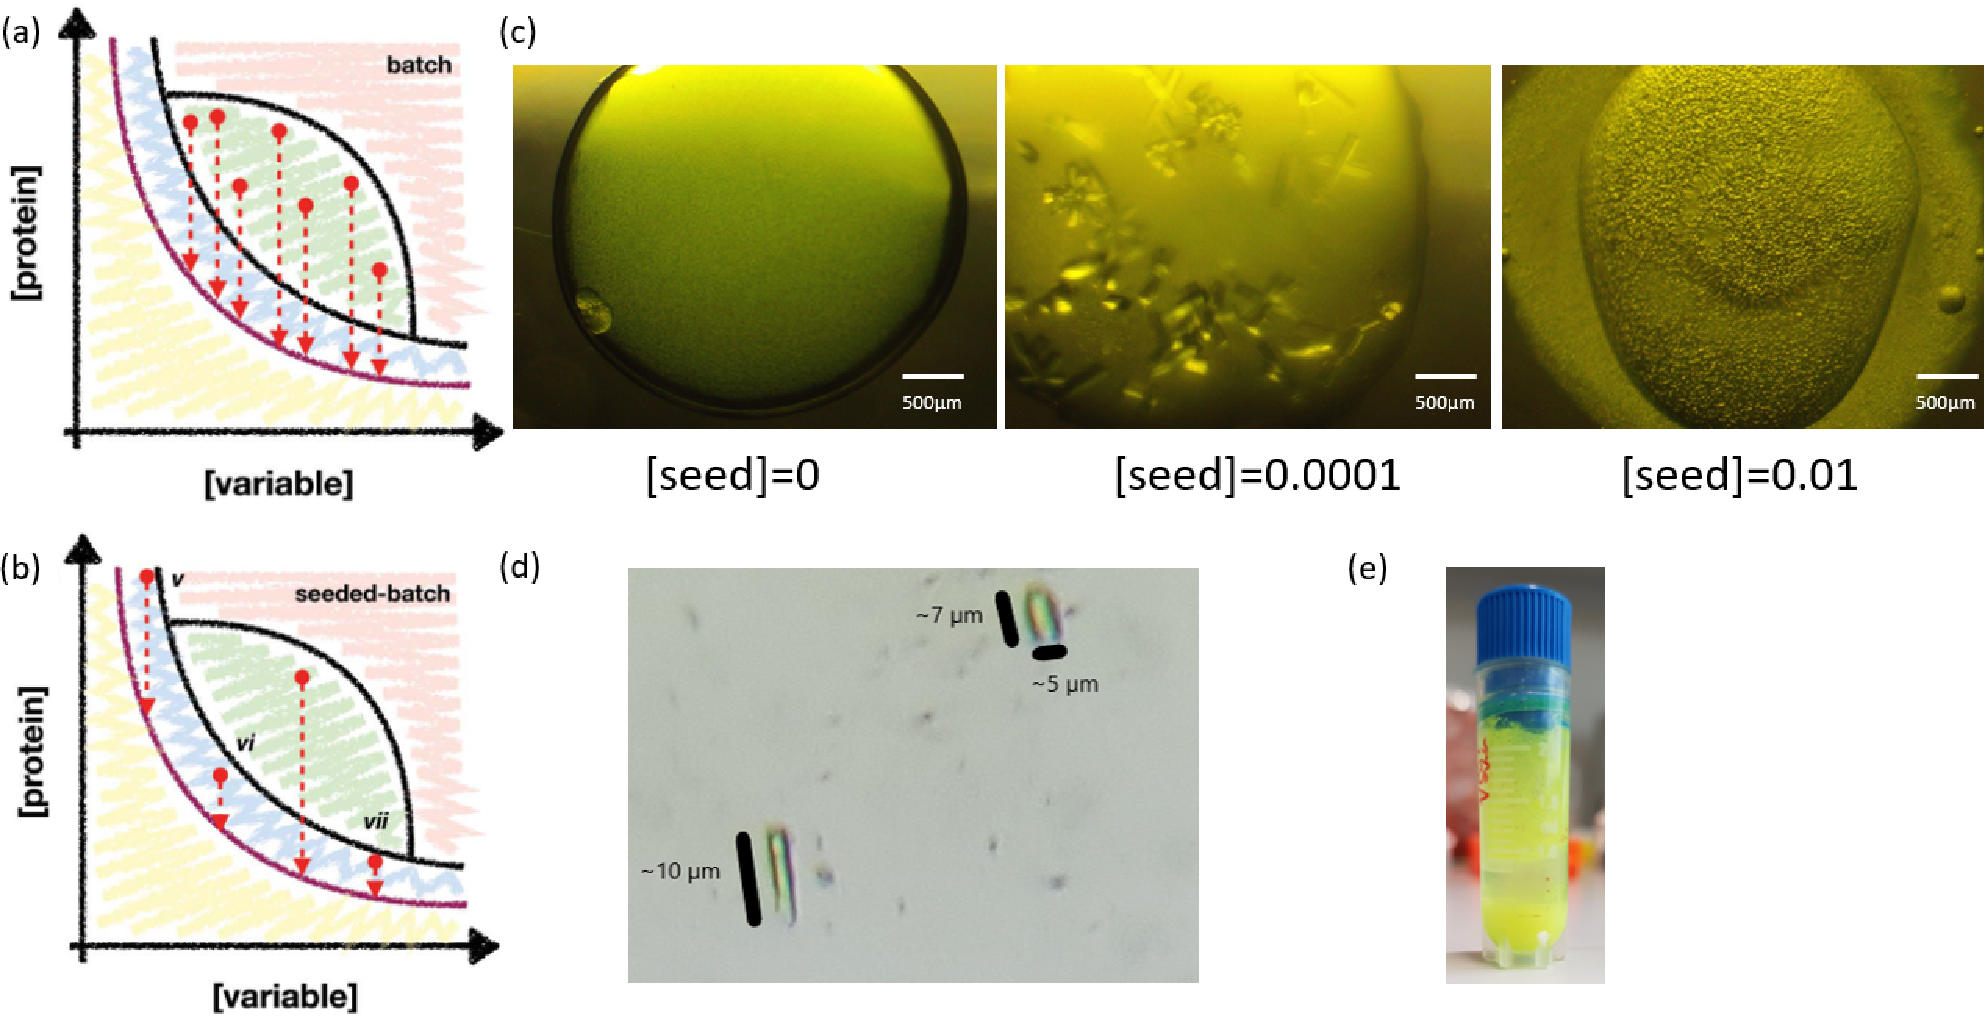
\includegraphics[width=\textwidth]{images/T-Cer/Crystallisation_T-Cer.pdf}
    \hfill
    \caption{Engineering microcrystals of T-Cer. (a) Schematic phase diagram of a batch crystallisation experiment. The nucleation zone is coloured in green, the meta-stable zone is coloured in blue and the precipitation zone is coloured in red. The red dotted arrow represents possible linear, downward trajectories taken by crystallisation batches as the concentration of protein in solution decreases with crystallisation. (b)  Schematic phase diagram of a seeded batch crystallisation experiment. The colour codes are unchanged from (a). The use of seeds allows to exploitation of a much larger zone of the phase diagram because hitting the nucleation zone is no longer needed since crystal growth can occur around seeds, as evidenced by trajectories V, VI and VII. Both (a) and (b) are reproduced from \cite{bealeSuccessfulSamplePreparation2019} (c) 10 \textmu l micro-batches of T-Cer set-up with identical crystallisation conditions (100 mM HEPES at pH 8.0;  20 \% PEG; 50 mM MgCl\textsubscript{2}; 1:3 protein), but seeded with increasing concentration of crystal seeds. If no seeds are added to the mix, only phase transition is visible in the batch. If 1 \textmu l of a 1/1000 diluted seed stock is added to the mix, \textasciitilde 50 large (\(100 \times 100 \times 50\) \textmu m\textsuperscript{3}) crystals grow. If 1 \textmu l of a 1/10 diluted seed stock is added to the mix, a slurry of micro-crystals grows.  (d) Crystals grown in the final conditions scaled for a batch volume of 1.5 ml (100 mM HEPES at pH 8.0;  25 \% PEG; 50 mM MgCl\textsubscript{2}; 1:3 protein), with a constant thickness of \textasciitilde 5 \textmu m. (e) Sample tube sent to PETRA III in prevision of the beamtime, with clear sedimentation of the crystal pellet.}
    \label{fig:Crystallisation_T-Cer}
\end{figure}
Crystal seeds of T-Cer were first prepared by crushing large (\textasciitilde 500 \textmu m) crystals fished from 12 hanging drop wells using a tissue grinder (protocol described in \parencite{aumonierTimeresolvedMonochromaticSynchrotron2019}). The large crystals were re-suspended in a solution with the same composition as their mother liquor and reference for 5 minutes. The resulting slurry was stored in an Eppendorf tube and characterised under a microscope. This approach is quick and straightforward, but large (> 10 \textmu m) particles remain in the solution, amid smaller barely visible seeds. This introduces inhomogeneity in the size distribution of crystals grown with seeded batches. To solve the size inhomogeneity issue, the large crystals harvested were crushed with ceramic seeding beads (Hampton research, HR4-781 - Seed Bead Ceramic Kit) instead of a tissue grinder. 6 seeding beads were added to an Eppendorf tube containing large crystals harvested and re-suspended in 200 \textmu l, before it was shaken for 25 minutes using a vortex 'hands-off' attachment, at medium speed to minimise friction-induced heat. The resulting seed suspension was observed under a microscope to validate that it contains only \textasciitilde  \textmu m or smaller particles.

Microbatches are medium-sized (10 \textmu l) droplets set in sitting drop plates, covered in oil to prevent evaporation (See \cite{chayenMicrobatchCrystallizationOil1992} for a precise description of the method). They were used to bridge the gap between known hanging drop vapour diffusion conditions yielding microcrystals of T-Cer and the desired batch condition.  Microcrystals of T-Cer can reliably be obtained via the hanging-drop vapour diffusion method with the following conditions: 30\% PEG 4000, 100 mM HEPES pH 8.0, 50mM MgCl2, 1/1 ratio of 20 mg/ml T-Cer. Arrays of micro-batch trials were started around this condition screening for protein concentration (by adjusting the protein/mother-liquor ratio of the mix) and precipitant concentration. The micro-batches were set in sitting drop plates to allow daily observation with a microscope.  It is possible to identify conditions where the concentration of T-Cer seeds governs crystal growth, as evidenced by the absence of crystal growth if no seeds are supplemented (first panel of Fig. \ref{fig:Crystallisation_T-Cer} (c)), and the strong variation in crystal size depending on the concentration of T-Cer seeds provided (visible in the second vs the last panel of Fig. \ref{fig:Crystallisation_T-Cer} (c)). If the desired state has been reached, the crystallisation can be 'quenched' by centrifuging the crystals at a moderate (3000 G) speed and resuspending them in a mother liquor of identical composition, without T-Cer.  Finally, the sedimentation of thin sand-like particles is a telltale sign of a successful batch crystallisation (Fig. \ref{fig:Crystallisation_T-Cer} (e)). 

These trials allowed to converge on an optimal condition of 20\% PEG 4000, 100 mM HEPES pH 8.0, 50 mM MgCl2, 1/1000 final dilution of the seed stock and 13.3 mg/ml final concentration of T-Cer for crystal growth.  This condition yielded crystals of a homogeneous thickness (5 \textmu m, Fig. \ref{fig:Crystallisation_T-Cer} (d)). Several sample tubes (Fig. \ref{fig:Crystallisation_T-Cer} (e)) were sent to PETRA III to plan the beamtime. Crystals were also grown on-site with the help of the P11 beamline staff, using seeds made from one of the sent batches, showcasing the robustness of this protocol. 

\subsubsection{Growing high-resolution diffracting crystals}\label{sec:highrescryst}

The size of the crystal was increased to further enhance the diffracting resolution. This was achieved by using a PEG concentration of 10 \%, too low to allow nucleation of the protein on its own (See Fig. \ref{fig:Crystallisation_T-Cer} (c)), and further decreasing the concentration of crystal seeds supplemented to 1/100 000. Protein concentration was maintained at 20 mg/ml. As a result, the sample which would have been used for the growth of many \textasciitilde 20-50 crystals was funnelled into the growth of 1 - 3 larger (\(\sim 200 \times 100 \times 100 \) \textmu m\textsuperscript{3}) crystals. Transferring a crystal into a drop of cryo-protectant causes mechanical stress, for instance, T-Cer and its variants' crystals melt when they are soaked in glycerol. As a final step, we used the crystallisation condition outlined above, supplemented with 20 \% V/V glycerol, and produced large, cryoprotected T-Cer crystals.

\subsubsection{Ammonium sulfate crystallisation condition to improve mixing}\label{sec:ammonium}

PEG, as a viscous agent, has been shown to inhibit the transfer of protons from the bulk solvent to the chromophore pocket of the GFP \parencite{saxenaProteinDynamicsControl2005}. This is due to PEG inhibiting protein dynamics and preventing the normal function of proton shuttling pathways. PEG also slows down the diffusion rate of small molecules in crystals and their mother liquor (\cite{makinenReactivityCryoenzymologyEnzymes1977}, Tomizaki Takashi (PSI), Sylvain Engilberge (IBS), personal communication \footnote{In particular, the diffusion rate of several coloured dyes in protein crystals and their mother liquor was assed with the acoustic levitation device currently being commissioned on PXI \parencite{tsujinoUltrasonicAcousticLevitation2016,kepaAcousticLevitationRotation2022}. Picoliter liquid dispensers were used to project droplets of dies on droplets containing protein crystals. The mixing time was assessed using a high-speed camera. Mixing times were noticeably higher (tens of seconds for PEG-based crystallisation conditions vs 100s of ms for salt-based conditions).}). PEG is also known to block substrate diffusion channels \parencite{barrettInsightsRedoxPartner2004}. T-Cer crystals are obtained in very high molecular weight (4000) PEG. These long molecules induce molecular crowding, which could also participate in slowing down the movements of the \textbeta-sheets in T-Cer and T-Cer-s crystals. 

Fluorescent proteins have been crystallised in salt-based conditions before. A survey of the Protein Data Base, as well as a personal communication from Nicolas Coquelle, directed me to the crystallisation condition of rsEGFP2 at neutral pH used for the TR-SFX measurements of \cite{coquelleChromophoreTwistingExcited2018}. However, T-Cer-s is significantly different from rsEGFP2. As a consequence, T-Cer transitioned from soluble to semi-amorphous particles (Fig. \ref{fig:T-Cer-NH4} (a)) without ever crystallising. Screening around the condition did not yield any crystalline particles. 

Based on the personal experience that rounds of seeding would improve the quality of crystals and microcrystals, a seeded crystallisation trial was prepared in a condition containing both PEG 4000 and ammonium sulfate, with seeds prepared from crystals grown in PEG-based conditions with the P 2\textsubscript{1} 2\textsubscript{1} 2\textsubscript{1} crystal packing. This trial proved that crystals could be grown if the crystallisation drop was seeded in a condition containing 15\% PEG and 0.5 M ammonium sulfate (Fig. \ref{fig:T-Cer-NH4} (b)). The crystals grown in these conditions were harvested to make a new preparation of crystal seeds (see Section \ref{sec:microcrystallisation} for the protocol). The process was repeated several times, with increments of 5 \% diminution of the concentration in PEG, and 0.25 M augmentation of the concentration in ammonium sulfate, and using the previous trial as a base for the preparation of seeds. The final condition contained only 100 mM of Hepes and 2 M ammonium sulfate and yielded satisfyingly sized homogeneous micro-crystals (Fig. \ref{fig:T-Cer-NH4} (c)). The size of the micro-crystals can be adjusted by varying the concentration of crystal seeds. 
\begin{figure}[H] %bt!]
    \centering
        \noindent 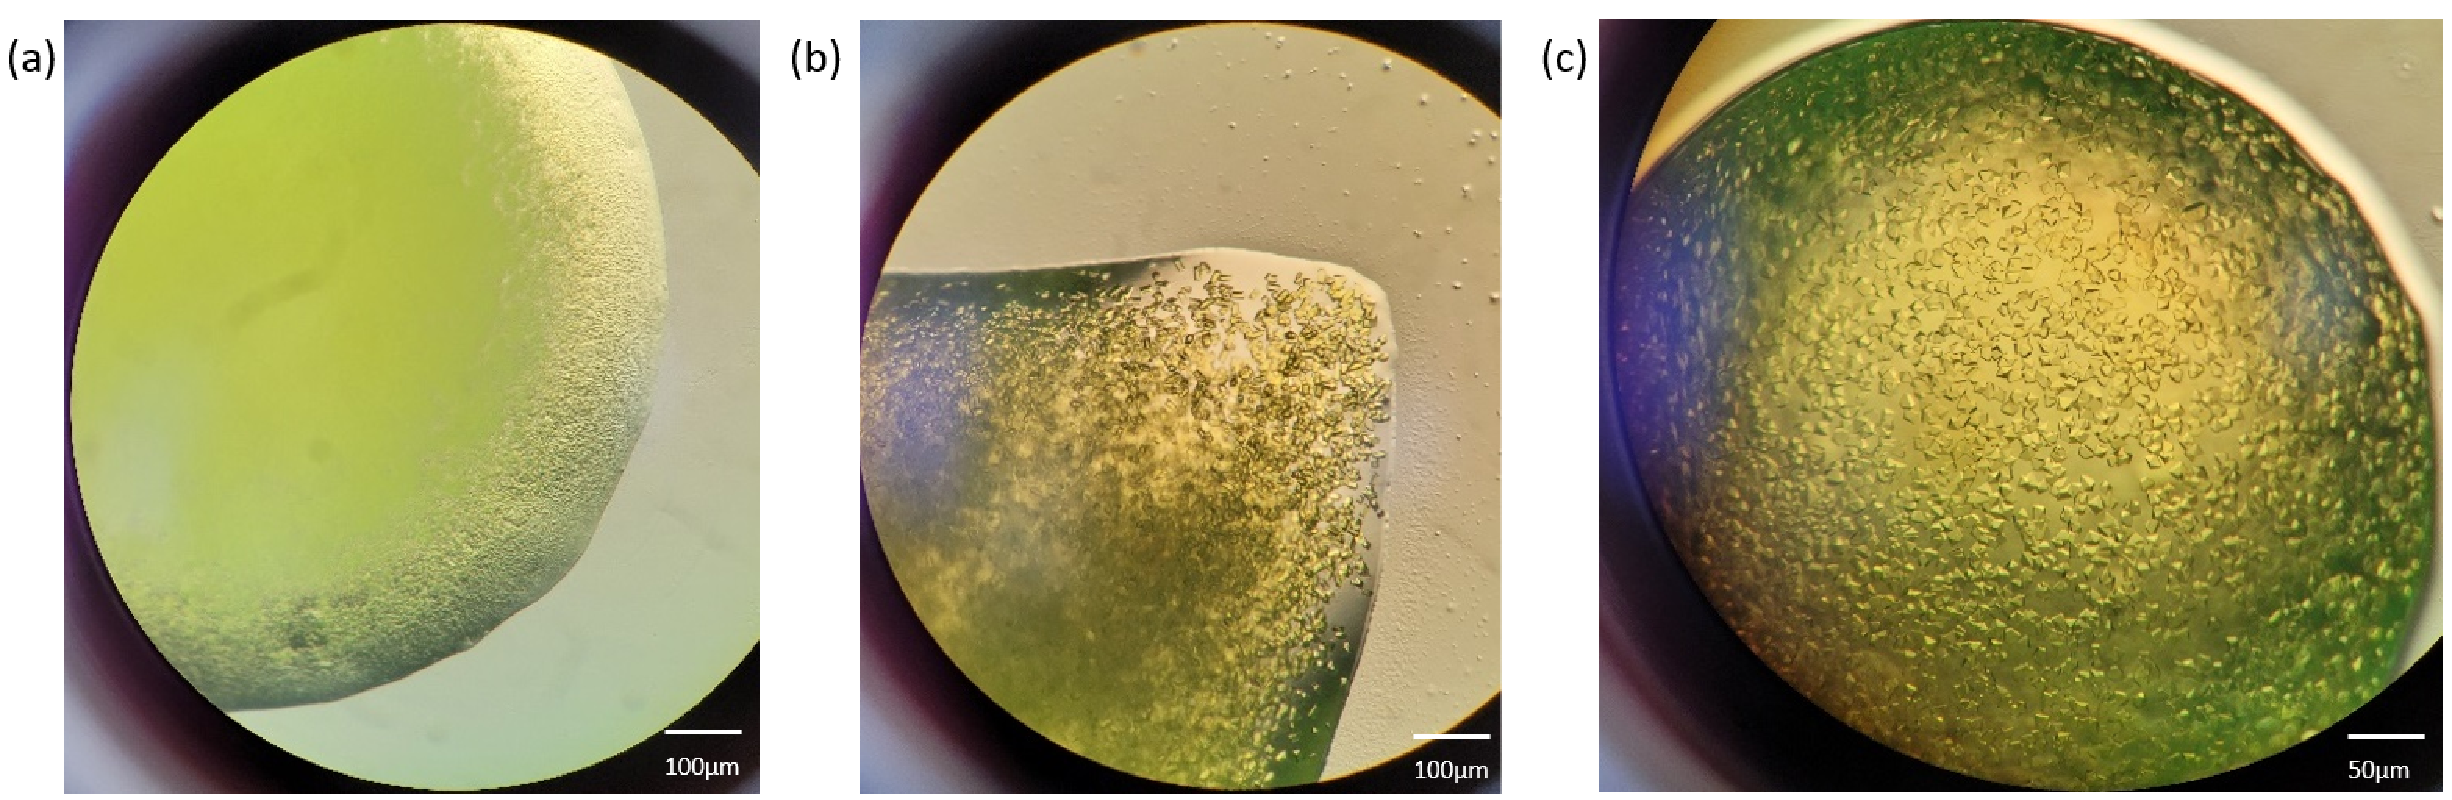
\includegraphics[width=\textwidth]{images/T-Cer/NH4_crystallisation_T-Cer-s.pdf}
    \hfill
    \caption{Engineering a crystallisation condition for T-Cer-s in ammonium sulfate. (a) Hanging drop vapour diffusion crystallisation trial of T-Cer-s. The mother liquor contains 100 mM HEPES pH 7.0 and 2 M ammonium sulfate. Only extremely small amorphous particles formed. The yellow colour of the particles indicates that T-Cer-s is not denatured. (b) Cross-seeded mixed precipitant crystallisation condition: the mother liquor contains 100 mM HEPES pH 7.0, 1M ammonium sulfate and 10 \% PEG 4000. It is seeded with T-Cer-s crystal seeds diluted 1/1000. Rectangular prism-shaped crystals (of size \(20 \times 20 \times 50 \) \textmu m\textsuperscript{3}) grew in 3 days, with a very homogeneous distribution of size.  (c) Ammonium sulfate only crystallisation condition: the mother liquor contains 100 mM HEPES pH 7.0 and 2 M ammonium sulfate. It is seeded with a preparation made from crystals grown in a mixed precipitant condition. Bi-pyramid-shaped microcrystals (of size \(20 \times 20 \times 20 \) \textmu m\textsuperscript{3}) grew in 3 days, with a very homogeneous distribution of size.}\label{fig:T-Cer-NH4}
\end{figure}
This crystallisation condition was ported to batch crystallisation with a 1:2 ratio of protein to mother liquor, a conserved final ammonium sulfate and pH buffer concentration, and a concentration of seeds divided by 3. 


\subsection{Limited proteolysis of T-Cer enhances its flexibility \textit{in crystallo}}\label{sec:limited_proteolysis}
The plasmid of T-Cer does not contain a cleavage site between the HIS-tag used for the affinity purification step and the rest of the protein, it is therefore not possible to remove it during the purification. Further, this HIS-tag is located at the C-terminus. As previously discussed (see Section \ref{sec:ageing}), the C-terminus of T-Cer adopts a different position depending on the pH. For crystals obtained at neutral pH (that is to say, all T-Cer crystals used for TR-MX experiments over the course of this project), the C-terminus is positioned away from the main \textbeta barrel of T-Cer, angled at 90 \degree. This tail is composed of semi-flexible (only the main chain is visible in the electron density map) and rigid (fully ordered, all of the amino acids are visible in the electron density) amino acids.  Upon examining the crystal packing of T-Cer at neutral pH, it appears that the C-terminal tail is stuck between neighbouring symmetry mates (Fig. \ref{fig:limited_proteolysis} (a)).  In particular, Y237 near the end of the C-terminus, is perfectly ordered and creates a crystal-contact point with the backbone of K45 from a symmetry mate. While not visible, the bulky HIS-tag is still present in the crystals and constitutes an additional source of crowding in that region of the unit cell.  

The appearance of the E,Z configuration of the chromophore after a pH drop likely requires the same movement of the 7\textsuperscript{th} strand as observed during the ageing phenomenon (Section \ref{sec:ageing}). This movement is hindered \textit{in crystallo}, which is likely in part a consequence of the rigidity of the C-terminus (Fig. \ref{fig:T_Cer_cter}). Therefore, removing the C-terminal tail of T-Cer from the protein before crystallisation might increase the flexibility of T-Cer in its crystalline form. 

Limited proteolysis has been utilised by the group of Antoine Royant (and its former members) to trim flexible parts of a protein and facilitate its crystallisation \parencite{aumonierTimeresolvedMonochromaticSynchrotron2019,gotthardCapturingBluelightActivated2023}.  In his thesis, Sylvain Aumonier describes the incubation of T-Cer with trypsin as a way to control the nucleation rate of the protein and improve his micro-crystallisation trials. The most 'accessible' part of T-Cer is its C-terminus; it is therefore likely that the main consequence of the limited trypsination of T-Cer was the removal of the tail. 

At the end of the purification, right before crystallisation, T-Cer was incubated with increasing concentration of Trypsin (5 \textmu g/ml to 5 mg/ml), and without Trypsin at 37 \degree C for 1h \footnote{This is a reproduction of the protocol detailed in Section 2.1.3 of \cite{aumonierTimeresolvedMonochromaticSynchrotron2019}. T-Cer is extremely thermostable (unfolding temperature of 84.8\degree C, unpublished data).}.  Running the incubated sample on an SDS-PAGE migration gel revealed the appearance of an additional, slightly lower molecular weight band (lanes 3:6 of Fig. \ref{fig:limited_proteolysis}) (b)) than the non-incubated proteins (lanes 1 and 8 of Fig. \ref{fig:limited_proteolysis}) (b)). This suggests that trypsin has indeed cleaved part of the protein, reproducing results of \cite{aumonierTimeresolvedMonochromaticSynchrotron2019}. 

Importantly, Trypsin self proteolyses extremely quickly. As an example, Trypsin incubated at 37 \degree C for 1h appeared as extremely low molecular weight fragments in SDS-PAGE migration. In order to obtain a band on the gel, Tryspin had to be loaded directly from the extemporaneously thawed stock, kept at 4\degree C  (lane 7 in Fig. \ref{fig:limited_proteolysis} (b)). It is therefore safe to assume that Trypsin has fully self-propolysed before the crystallisation batch is set. 
\begin{figure}[H] %bt!]
    \centering
        \noindent 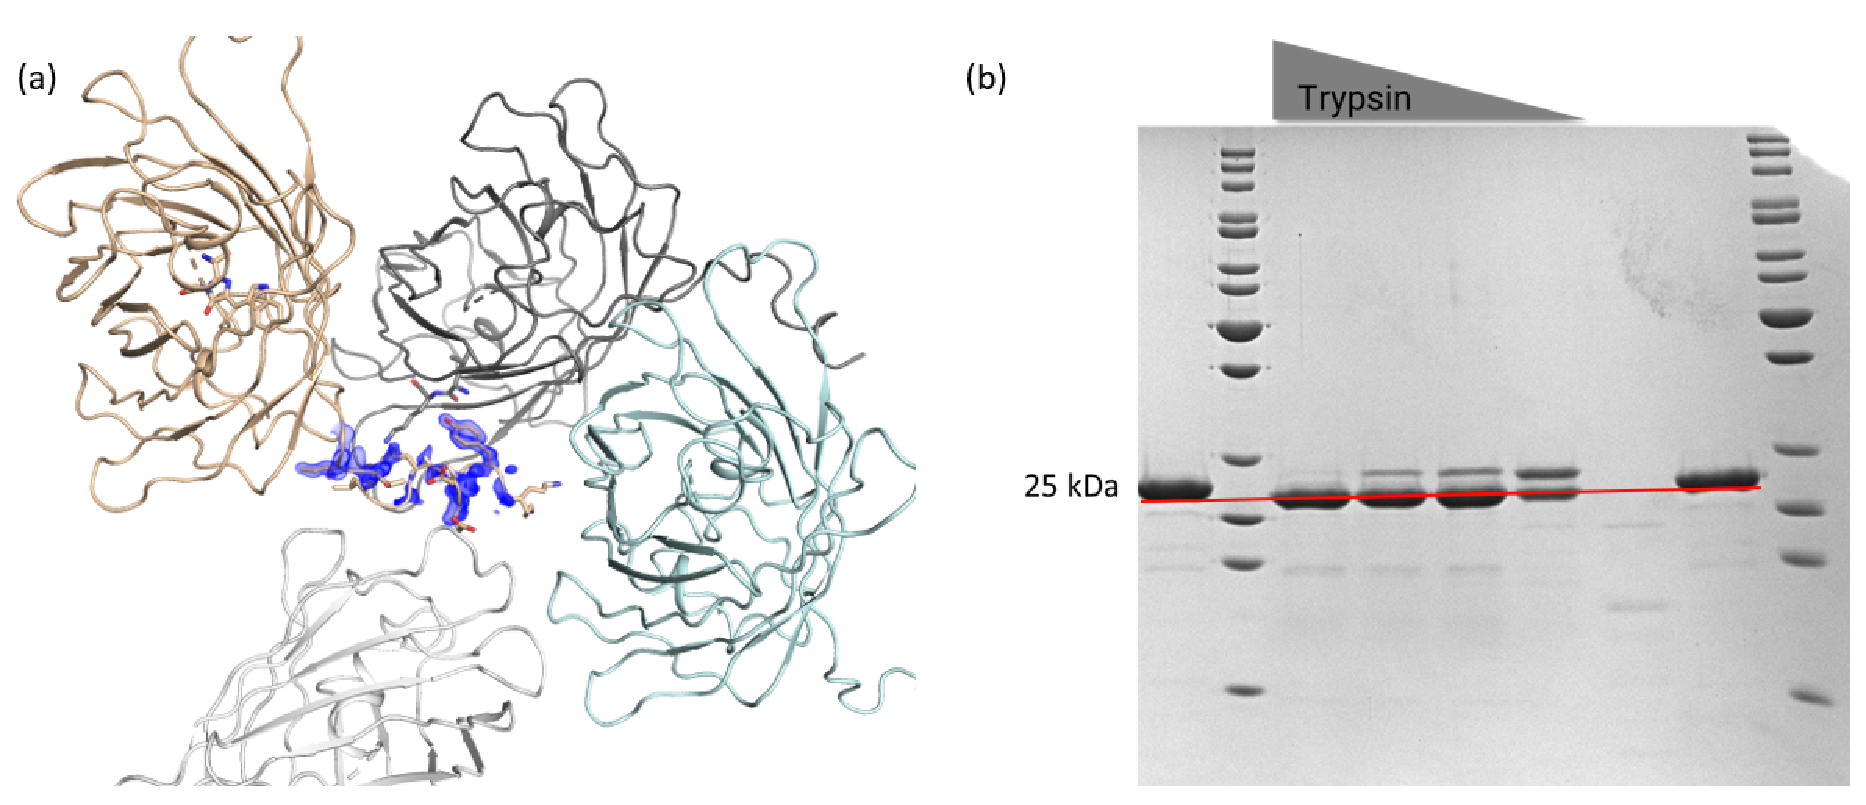
\includegraphics[width=\textwidth]{images/T-Cer/Limited_proteolysis.pdf}
    \hfill
    \caption{Limited proteolysis to remove the C-terminal tail of T-Cer. (a) Structure of symmetry-related molecules in a neutral-pH crystal of T-Cer. The electron density (2\(F_{obs} - F_{calc}\), 1.11 \AA\  resolution) map is represented on its C-terminal tail contoured at 1 \textsigma\ level Three of its symmetry mates (grey, pale-cyan and white) are also represented. The C-terminal tail of T-Cer at neutral pH is trapped between three symmetry mates, rigidifying it. Tyrosine 237 establishes an H-bond with the carbonyl of Lys 45 from the grey monomer, further stabilising it. This interaction is  a crystal packing point. (b) SDS-Page migration of purified T-Cer. Lanes contain (from left to right):\\
    1. T-Cer incubated at 37 \degree C without Trypsin\\
    2. Molecular weight ladder\\
    3. T-Cer and 1/10 diluted Trypsin stock\\
    4. T-Cer and 1/50 diluted Trypsin stock\\
    5. T-Cer and 1/100 diluted Trypsin stock\\
    6. T-Cer and 1/1000 diluted Trypsin stock\\
    7. Trypsin from the stock (non-incubated)\\
    8.T-Cer incubated at 37 \degree C without Trypsin\\
    9. Molecular weight ladder\\
    The red bar shows the migration front from both full-length T-Cer lanes. All conditions of T-Cer incubated with Trypsin (lanes 3:6) showcase a band of slightly lower molecular weight than non-incubated T-Cer, presumably cleaved T-Cer. Lanes  4,5 and 6 show an increasingly weaker band of the same molecular weight as non-cleaved T-Cer. The lower molecular weight band grows with Trypsin concentration, and the T-Cer molecular weight band decreases with Trypsin concentration.}\label{fig:limited_proteolysis}
\end{figure}
In preparation for the Hamburg trip, large crystals of T-cer cleaved with the protocol described above, obtained at neutral pH, were soaked in 1 M pH 4.0 Sodium Citrate buffer and cryo-cooled after a minute. They exhibited shrunken lattice parameters, which was an improvement from the results of previous soaking experiments (described at the end of Section \ref{sec:ageing}). This suggested that using pure pH buffer for the pH drop and limited proteolysis for sample preparation were indeed improvements to the protocol.

In addition to the micro-crystalline sample of T-Cer sent to Hamburg from Grenoble, T-Cer was also expressed, proteolysed and crystallised onsite directly to ensure sample quality. 

\subsubsection{Effect of the proteolysis on the lattice parameter distribution}
The C-axis of the unit cell in REF-LAMA and REF-P11-2 (crystallised with proteolysed T-Cer) is 72.6 \AA\ long (Table \ref{tab:structure-list}), a 2 \AA\ increase compared to that of REF-TPD-1 (crystallised with full-length T-Cer, Table \ref{tab:structure-list}), which supports the idea that the limited proteolysis step affects the protein packing. Otherwise, REF-LAMA is identical to REF-TPD-1 and REF, which validates that the proteolysis step does not affect the chromophore pocket. 

3 s after proteolysed crystals are shot with a droplet of sodium acetate, distinct populations (70 \AA\ long C-axis and 66.8 \AA\ long C-axis) are observed in the distribution of lattice parameters (Table \ref{tab:structure-list}). 3S-LAMA corresponds to the most abundant, short-axis population. 

The same phenomenon occurs 3 s and 8 s after proteolysed crystals are mixed with sodium acetate (Table \ref{tab:structure-list}).  Interestingly, the mix of population is only observed 3 s after mixing with sodium citrate, and the 8 s population distribution is homogeneous (short axis). 3S-TPD-Ac, 3S-TPD-Ci and 8S-TPD-Ac correspond to the 66.8 \AA\ population.

The existence of several species in the distribution of lattice parameters during serial data processing with CrystFEL is puzzling. This may be a consequence of an inhomogeneous cleavage of the C-terminus by the limited proteolysis step, leading T-Cer to form crystals made of monomers all cleaved in the same way, which difference is only visible once their crystalline lattice has been deformed by the pH drop. 

\subsection{A truncated T-Cer construct with enhanced flexibility \textit{in crystallo}}\label{sec:short}

Removing the C-terminus of T-Cer via limited proteolysis increased the flexibility of T-Cer \textit{in crystallo}. However, the precise cleavage site of Trypsin could not be identified in structures of proteolysed crystals, and the limited proteolysis might have created different populations in the distribution of lattice parameters after the pH drop (Section \ref{sec:discussion_P11_2}). To more reliably produce flexible crystals, a construct where this C-terminus is lacking was ordered. 

\subsubsection{Constructs design}
The T-Cer construct used so far (described in \cite{aumonierTimeresolvedMonochromaticSynchrotron2019}) did not feature a TEV cleavage site between the purification HIS-tag and the main body of the protein. Any new constructs ordered would have to include such a site so that the tag could be removed before crystallising. However, T-Cer is extremely thermo-stable with a melting point temperature of \( 84.8 \pm 0.2 \degree C \) (unpublished data). The affinity chromatography step in the purification protocol of T-Cer (Section \ref{sec:T-Cer_methods}) can therefore be replaced with an incubation at high temperature to precipitate remaining contaminants. This approach prevents the introduction of 'non-physiological' sequence elements (the HIS-tag or the trailing ends of a cleavage site) in the construct. 

Exactly how short GFP family fluorescent protein can be has been investigated in the past to create more easily expressing proteins. For the GFP, amino acids 7 to 229 are needed for proper autocatalytic cyclisation of the residues forming the chromophore, and therefore, for the fluorescence \parencite{liDeletionsAequoreaVictoria1997}. T-Cer is considerably different from the GFP, and truncation of the N-terminus wasn't needed per se. Therefore, the truncated construct of T-Cer (T-Cer-s) was ordered from amino acids 1-229.

A variant of T-Cer-s with an HIS-tag and a TEV cleavage site in the N-terminal position was ordered as a fallback solution.

\subsubsection{Purification of T-Cer-s}

Expression and Cell lysis of T-Cer-s are carried out with the same protocol as T-Cer (Section \ref{sec:T-Cer_methods}), except DNAse is replaced with benzonase. This change is needed since soluble strands of DNA will withstand the heat shock and remain as contaminants. The bulk of them have to be cleaved or removed before any column-based purification step because of the risk of clogging or damaging the columns. Even then, long strands of DNA remain in the soluble fraction, as evidenced by the blurring of bands on the SDS-PAGE gel migration represented on the second track of Fig. \ref{fig:T-Cer-s_purif} (a). 

Immediately after the soluble fraction has been isolated, it is incubated at 80 \degree C for 20 minutes. The incubated sample is centrifuged at 20 000 G for 10 minutes at room temperature, and the supernatant is isolated. After the heat shock, an important amount of  protein contaminants remain as evidenced by the many bands present on track 5 of the SDS-PAGE gel migration represented in Fig. \ref{fig:T-Cer-s_purif} (a). An additional ammonium sulfate precipitation has thus been added to the protocol. 

To perform ammonium sulfate precipitation, the supernatant is transferred in a beaker with a stirring magnet at room temperature. Ammonium sulfate is incrementally added until the solution reaches 2 M. The suspension is then centrifuged again at 20 000 G for 10 minutes at room temperature, and the pellet (containing mostly contaminants) is discarded. Ammonium sulfate is added again until the solution reaches 2.2 M, causing T-Cer-s to precipitate. After centrifugation at 20 000 G for 10 minutes at room temperature, a visual inspection can validate that T-Cer-s is fully in the pellet (it is yellow-coloured). The isolated pellet is resuspended in 100 mM Tris pH 7.0, then dialysed overnight to remove salts. 

An anion exchange chromatography is used to remove left-over protein contaminants and pieces of DNA. The pH of the storage buffer for T-Cer-s was changed from pH 8.0 to 7.0 so that it would be 1.5 above its isoelectric point (5.5) and therefore allow anion exchange. The sample is loaded on the column, and nucleic acids (evidenced by the high 260 nm (purple) / 280 nm (blue) ratio of the first peaks in chromatogram in Fig. \ref{fig:T-Cer-s_purif} (b) as well as the absence of bands on lanes 6-7 of the gel presented in (b))  flow through. Then a gradient from 0 to 20\% of 1.5M NaCl is used to remove remaining contaminants (fractions 58-64 on Fig. \ref{fig:T-Cer-s_purif} (b), contaminant bands visible on lanes 8. and 9. of (a)), forming two distinct peaks. T-Cer-S unbinds at 17 \% (255 mM NaCl), forming an elongated absorbance peak at 435 nm (Fig. \ref{fig:T-Cer-s_purif} (b)). 

After anion exchange, the sample still contains visible traces of protein contaminants (Fig. \ref{fig:T-Cer-s_purif} (b), track 11.). A final step of size-exclusion chromatography with the same protocol as T-Cer (Section \ref{sec:T-Cer_methods}) is used to remove them.
\begin{figure}[H] %bt!]
    \centering
        \noindent 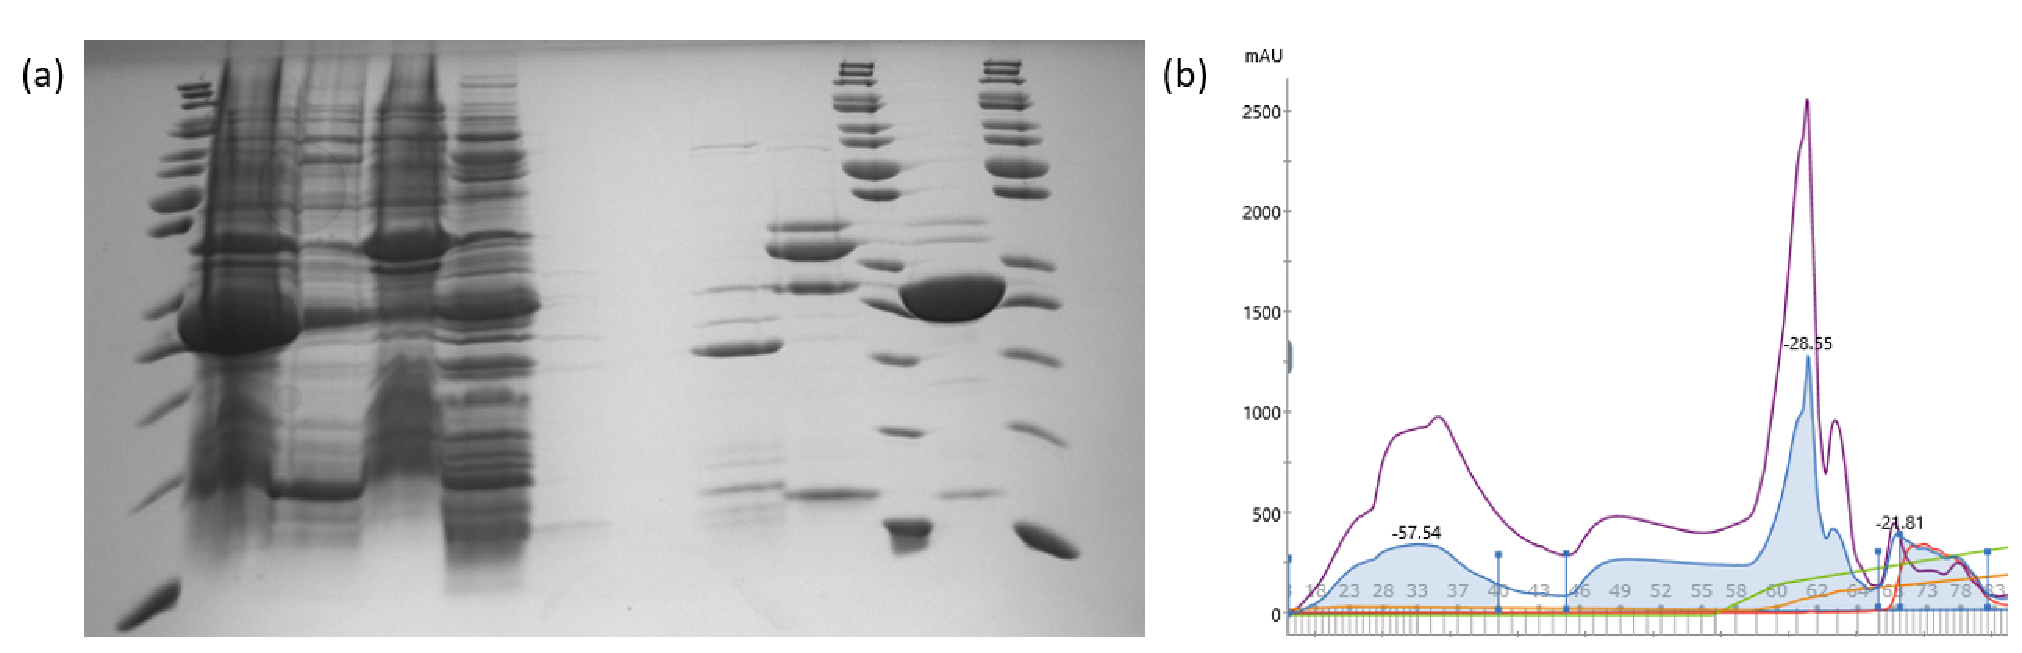
\includegraphics[width=\textwidth]{images/T-Cer/T-Cer-s_purification.pdf}
    \hfill
    \caption{Additional purification steps for T-Cer-s. (a) SDS-Page gel-migration of the sample over the purification protocol:
    1. Molecular Weight Ladder
    2. Soluble fraction after expression 
    3. Non-soluble fraction after expression 
    4. Heat precipitated fraction 
    5. Post heat shock supernatant 
    6. Anion exchange chromatography: fraction 33 (flow-through)
    7.  Anion exchange chromatography: fraction 49 (Wash)
    8. Anion exchange chromatography: fraction 61 (first contaminant peak)
    9. Anion exchange chromatography: fraction 63 (second contaminant peak)
    10. Molecular Weight Ladder
    11. Anion exchange chromatography: fraction 70-82 T-Cer-s peak
    12.  Molecular Weight Ladder
T-Cer-s is present in the soluble fraction after expression. This supernatant is still heavily contaminated and contains strands of nucleic acids (blurring of the bands on track 2). T-Cer-s is the most abundant protein after heat shock (25 kDa band on track 5), but a lot of contaminant proteins remain. The peak isolated using the specific absorbance peak of T-Cer-s still contains small amounts of contaminants. 
    (b) Chromatogram of the anion exchange purification step, the x-axis is volume, grey markings are fractions. Absorbance at 260 nm (nucleic acids) is plotted in purple, Absorbance at 280 nm (proteins) in blue, concentration of NaCl (0-1.5M), and Absorbance at 435 nm (T-Cer-s main absorbance peak) in red. The flow-through and wash fractions (0-55) exhibit a high UV260/UV280 ratio and no band on the SDS-PAGE track corresponding, indicating the presence of nucleic acids. The first and second peaks appearing during the gradient exhibit a constant UV260/UV280 ratio; they contain mostly protein contaminants which are visible on the SDS-PAGE migration on lanes 8 and 9. Finally, fractions 70-82 contain T-Cer-s, as evidenced by the peak of absorbance at 435 nm.}\label{fig:T-Cer-s_purif}
\end{figure}
The crystals used for the soaking experiments (Section \ref{sec:soaking}) were of size \(\sim 200 \times 50 \times 50 \) \textmu m\textsuperscript{3}, to reproduce the conditions of the upcoming ALD beamtime on beamline PXI (Section \ref{sec:ALD}). 
\subsubsection{Soaking and cryo-trapping}

T-Cer-s crystals were first soaked in 0.8 M pH 4.0 pH buffer, 20\% glycerol (for cryo-protection) then cryo-cooled after set delays by plunging them in liquid nitrogen. Strikingly, crystals of T-Cer grown in ammonium sulfate seemed to tolerate 20 \% glycerol much better than crystals grown in PEG. The crystal structures were collected on beamline ID23-2 at the ESRF \parencite{nanaoID232AutomatedHighperformance2022}. The electron density maps of all crystals soaked for shorter than 150 s did not exhibit features supporting the presence of the E,Z configuration (which is why only 150S-CT-S is shown. 

The identification of this very low (\textasciitilde 10 \%) occupancy of the E,Z state in 150S-CT-S was helped by the good diffraction resolution (1.3 \AA\ after soaking) of the crystals. This is an undeniable sign that the Z,Z to E,Z configuration switch can happen inside of a crystal. However, datasets cryo-trapped after 150 s do not contain more of the E,Z configuration. 

For V150A crystals, a very short soak was achieved by rapidly passing the crystal through a drop of 20\% glycerol, 0.8 M sodium citrate at pH 4.0, and immediately mounting it on the axis on BM07-FIP2. The (conservatively) estimated delay between the beginning of soaking and the cryo-cooling is 10 s. Because the crystal had not been co-crystallised with glycerol and because the pH drop visibly damaged it, the crystal diffracted to a slightly lower 1.3 \AA\ resolution. 

\subsubsection{Soaking and room-temperature collection}\label{sec:soaking_protocol}

The crystals were soaked for 1 minute in 1 M pH 4.0 sodium citrate buffer and then mounted on beamline ID30a3 - MASSIF3 \parencite{vonstettenID30A3MASSIF3Beamline2020} at room temperature, under the stream of a humidity controller \parencite{sanchez-weatherbyImprovingDiffractionHumidity2009}. Rotation diffraction datasets were collected after a set delay (comprising the time needed to search and lock the experimental hutch of the beamline). The collection of a complete dataset for T-Cer-s crystals takes 1.4 s, which is negligible compared to several-minute delays. The flux of the beamline was limited to 10 \%, in the 16 mA filling mode of the ESRF storage ring, so that the total dose deposited during a dataset would not exceed 300 kGy, to minimise global radiation damage while maintaining resolution. The dose was calculated with RADDOSE3D \parencite{zeldinRADDOSE3DTimeSpaceresolved2013}.

Because of the lower flux, and inherent lower order at room temperature, the diffraction resolution of collected datasets was moderate, 2.2 \AA\ at best. 

Importantly, this soaking protocol is not robust: soaking for more than 150 seconds is needed to observe electron density features of the E,Z configuration, but past that point, there seemed to be no correlation between soaking time and the occupancy of the fully converted species in the crystals. Further, some crystals never exhibited signs of the E,Z configuration, no matter how long their soaking time was. Crystals of T-Cer-s were also extremely brittle and sensitive to mechanical stress during and after the soak in pH 4.0 buffer (with or without glycerol) and any movement was liable to break them into very fine pieces.  Probably, the presence of turbulence in the droplet of pH buffer used to soak the crystal at the very beginning of the soak is needed to maximise the diffusion rate, but too much turbulence will kill the crystals.

A high level of humidity (99 \%) had to be maintained for the isomerization to happen at room temperature. The dependency on humidity was so pronounced that crystals mounted in an orientation where the loop was not perpendicular to the humid air stream, and which were shielded from the humid air flow stopped evolving, and never exhibited signs of the E,Z configuration. 

\subsection{Variant V150A of T-Cer-s}

A variant where V150 from the His-tagged version of T-Cer-s (See Section \ref{sec:short} for a description of the plasmids) is replaced by an Alanine was designed. The choice of mutating V150 to an alanine instead of a glycine was motivated by the need to keep a certain level of constraint around the chromophore so that it would still adopt the Z,Z configuration at neutral pH.  T-Cer-s was chosen as a scaffold to maximise the \textit{in crystallo} flexibility. Finally, there was no guarantee that this variant would retain the high thermo-stability of T-Cer. This is why variant V150A of T-Cer-s (V150A) was ordered with a HIS-tag. 

V150A was expressed and purified in the same conditions as T-Cer (Section \ref{sec:T-Cer_methods}). 

 The first V150A crystals were obtained via cross-seeding from T-Cer crystals, using the crystallisation conditions described in Section \ref{sec:T-Cer_methods}, with the same methodology that was used to obtain crystals of T-Cer-s with space group P 2\textsubscript{1} 2\textsubscript{1} 2\textsubscript{1} (Section \ref{sec:newspacegroup}). A seed solution prepared from the first V150A crystals was used for a second round of crystallisation. 

For high-resolution data collection on BM07-FIP2, V150A was crystallised using the methodology described in Section \ref{sec:highrescryst}. Rectangular prism-shaped crystals grew over a week.

\section{X-ray data collection}
For cryogenic-temperature (100 K) data collection, T-Cer and variants crystals are cryo-protected in their mother liquor, supplemented with 20 \% glycerol. While Cerulean crystals tolerate soaking in ethylene glycol better than glycerol, ethylene glycol binds inside the chromophore pocket and alters the spectroscopic properties of the protein \parencite{vonstettenAlterationFluorescentProtein2012}. The crystals were cryo-cooled by plunging them in liquid nitrogen. 

\subsection{Collecting high-resolution structures with a flat beam flat beamline BM07-FIP2}\label{sec:highrescol}
Tuning the crystal size with the method described in Section \ref{sec:highrescryst} enabled us to collect them on BM07-FIP2 (FIP2). FIP2 uses one of the bending magnets of the synchrotron, instead of an undulator \footnote{All MX beamlines of the structural biology group of the ESRF, as well as P11 and P14 /P14-2 at DESY use undulators as X-ray sources, because they produce a more focused flux.}. Bending magnets produce a more modest flux (\(\sim5 \times 10^{11}\) photons/s), and a less focused beam. The optics of FIP2 are designed to produce a nearly flat beam profile \footnote{As opposed to the gaussian shaped beam profile of the other beamline in the structural biology group of the ESRF}, with a considerably larger focal cross section (\(\sim200 \times 200 \) \textmu m\textsuperscript{3}, which can then be cut by slits). With a flat beam profile, the X-ray dose is homogeneously deposited into the crystal volume, making the most of it. The increased diffracting volume in turn allows the collection of a full dataset on a lower dose budget without compromising the diffracting power. Operating on a tight dose budget is important to collect a high-resolution MX structure, as high-resolution reflections are most sensitive to global radiation damage \parencite{garmanRadiationDamageMacromolecular2010}. Finally, crystals were collected with a reduced flux (\(\ 7.3 \times 10^{10}\) photons/s), long exposure time collection (1 s per image) strategy, which is optimal for high resolution (Aswin Chari, Gleb Bourenkov, personal communication), producing the structures presented in Section \ref{sec:V150A}.

Teasing these apart the configuration of the chromophore and conformations of the amino acids in the chromophore pocket of 8-V150A and 4-V150A was only possible because of the very high resolution (1 \AA\ resolution, but limited by the position of the detector of BM07-FIP2 and the X-ray photon energy, 12.8 kEv, at the time of the collection). 

\subsection{UV-vis absorption spectroscopy}

\subsubsection{In solution spectroscopy}
Spectra of T-Cer in solution at different pH points were recorded using a two-beam spectrophotometer (Jasco V-530), in a quartz cuvette, at a concentration of 0.8 mg/ml, in a buffer consisting of 100 mM HEPES (pH 8.0:7.0) or 100 mM MES (pH 6.5:6.0) or 100 mM sodium citrate (pH 5.5:4.0).

\subsubsection{\textit{ic}AS}
Unfortunately, the \textit{in crystallo} UV-vis absorption spectroscopy spectrum of 150-CT-S (Fig. \ref{fig:T-Cer-soak-struc} (a)) was hard to read because several rounds of mounting and dismounting on the beamline and on \textit{ic}OS had caused ice to form. 

To replicate it, spectra of T-Cer crystals were recorded on the main setup of the \textit{ic}OS platform, at the ESRF \parencite{vonstettenCrystalloOpticalSpectroscopy2015}, while maintained at 100K by a cryo-stream (Oxford 800). The crystals were cryocooled in liquid nitrogen and cryoprotected with glycerol. 

To time the transition between the configurations of the T-Cer-s chromophore, smaller (\(\sim 100 \times 20 \times 20 \ \) \textmu m\textsuperscript{3}) T-Cer-s crystals were grown at pH 8.0, and soaked in in 0.8 M pH 4.0 pH buffer then cryo-cooled on the cryo-stream of the \textit{ic}OS lab main setup 

sGS-CT (coloured blue in Fig. \ref{fig:T-Cer-soak-struc} (a)) is only slightly blue-shifted compared to sGS ( full line in Fig. \ref{fig:T-Cer_pH8vs4}), with a two-peaked absorption band maximised at 440 and 467 nm. 

\parencite{vonstettenCrystalloOpticalSpectroscopy2015} so that \textit{ic}AS could be measured (Fig. \ref{fig:T-Cer-soak-struc} (c)).

\subsection{Sample environment and endstations used}
\subsubsection{The CFEL tape drive mounted on beamline P11}\label{sec:presenting_tpd_P11}

Beamline P11 is a standard high-throughput MX beamline, with a focused beam size of \(4 \times 9 \) \textmu m\textsuperscript{3}, and a flux of \(10^{13}\) photons/s, at an energy level of 12 keV. It is operated by the Deutsches Elektronen-SYnchrotron (DESY). P11 can accommodate a TR-SSX setup, called the CFEL tape drive \parencite{beyerleinMixanddiffuseSerialSynchrotron2017,zielinskiRapidEfficientRoomtemperature2022}. This particular setup is suited for mixing-collection delays from the 100s of ms to the tens of seconds and allows fast mixing.

Diffusion of small molecules in crystals occurs on the us-ms timescale \parencite{makinenReactivityCryoenzymologyEnzymes1977}. Further, protein crystals are obtained in solutions often containing high concentrations of salt or viscous precipitant, further slowing down diffusion. This is why specific experimental setups have been developed to initiate reactions in crystals via diffusion. Two main approaches can be retained for this: 

\begin{itemize}
    \item A microfluidic setup specifically designed to create turbulence and mix a substrate solution with a suspension of crystals via convection. 
    \item Depriving the crystals of their mother liquor to bathe them in a solution containing the substrate. 
\end{itemize}

Both these approaches have weaknesses: nozzles designed to create turbulence are also prone to clogging and require that crystals do not exceed a specific size, whereas depriving the crystals of their mother liquor means specific devices must be used to maintain their hydration level. 

The tape drive setup was developed by the team of Dominik Oberthür at the Centre for Free Electron Laser Science (CFEL, Hamburg). \parencite{beyerleinMixanddiffuseSerialSynchrotron2017,zielinskiRapidEfficientRoomtemperature2022} relies on the first approach. For the experiment, two 70 um glass capillaries are plugged into a fast-mixing nozzle. Capillary 1 (left in Fig. \ref{fig:tape drive}) contains the suspension of microcrystals and is inserted in the nozzle. Capillary 2 (right in Fig. \ref{fig:tape drive}) contains an acidic pH solution which will be mixed with the crystal slurry to lower the pH of the crystals. Both capillaries are plugged into a fast-mixing nozzle (red zoomed rectangle in Fig. \ref{fig:tape drive}). This nozzle is designed to create a turbulent flow at the point of contact of both channels to minimise the mixing time. The mix is immediately deposited on a tape which is rolled to bring the sample to the point of interaction with the X-ray beam (yellow in Fig. \ref{fig:tape drive}). Both tape speed and the distance between the position of the beam and that of the point of deposit of the tape can be adjusted, allowing precise control over the delay between the beginning of mixing and exposure to the X-ray beam. With this technique, time points from 300 ms to tens of seconds can be achieved. Of note, this does not take into account the mixing and \textit{in crystallo} diffusion times, which might exceed 300 ms. 
All variables (tape speed, flows of each capillary, nozzle-beam distance) of the experiments are controlled in a graphical interface. The flow of each capillary must be adjusted to prevent clogging while still allowing fast mixing. This last parameter must be optimised ahead of the actual data collection and adjusted during the beamtime. 
Finally, live indexing feedback is provided. Live indexing is ubiquitously used as the primary feedback on a serial crystallography experiment (see Section \ref{sec:dataprocan}). It can validate that crystals are indeed being shot by the X-ray beam and that they diffract to an appropriate resolution. 

\begin{figure}[H] %bt!]
    \centering
        \noindent 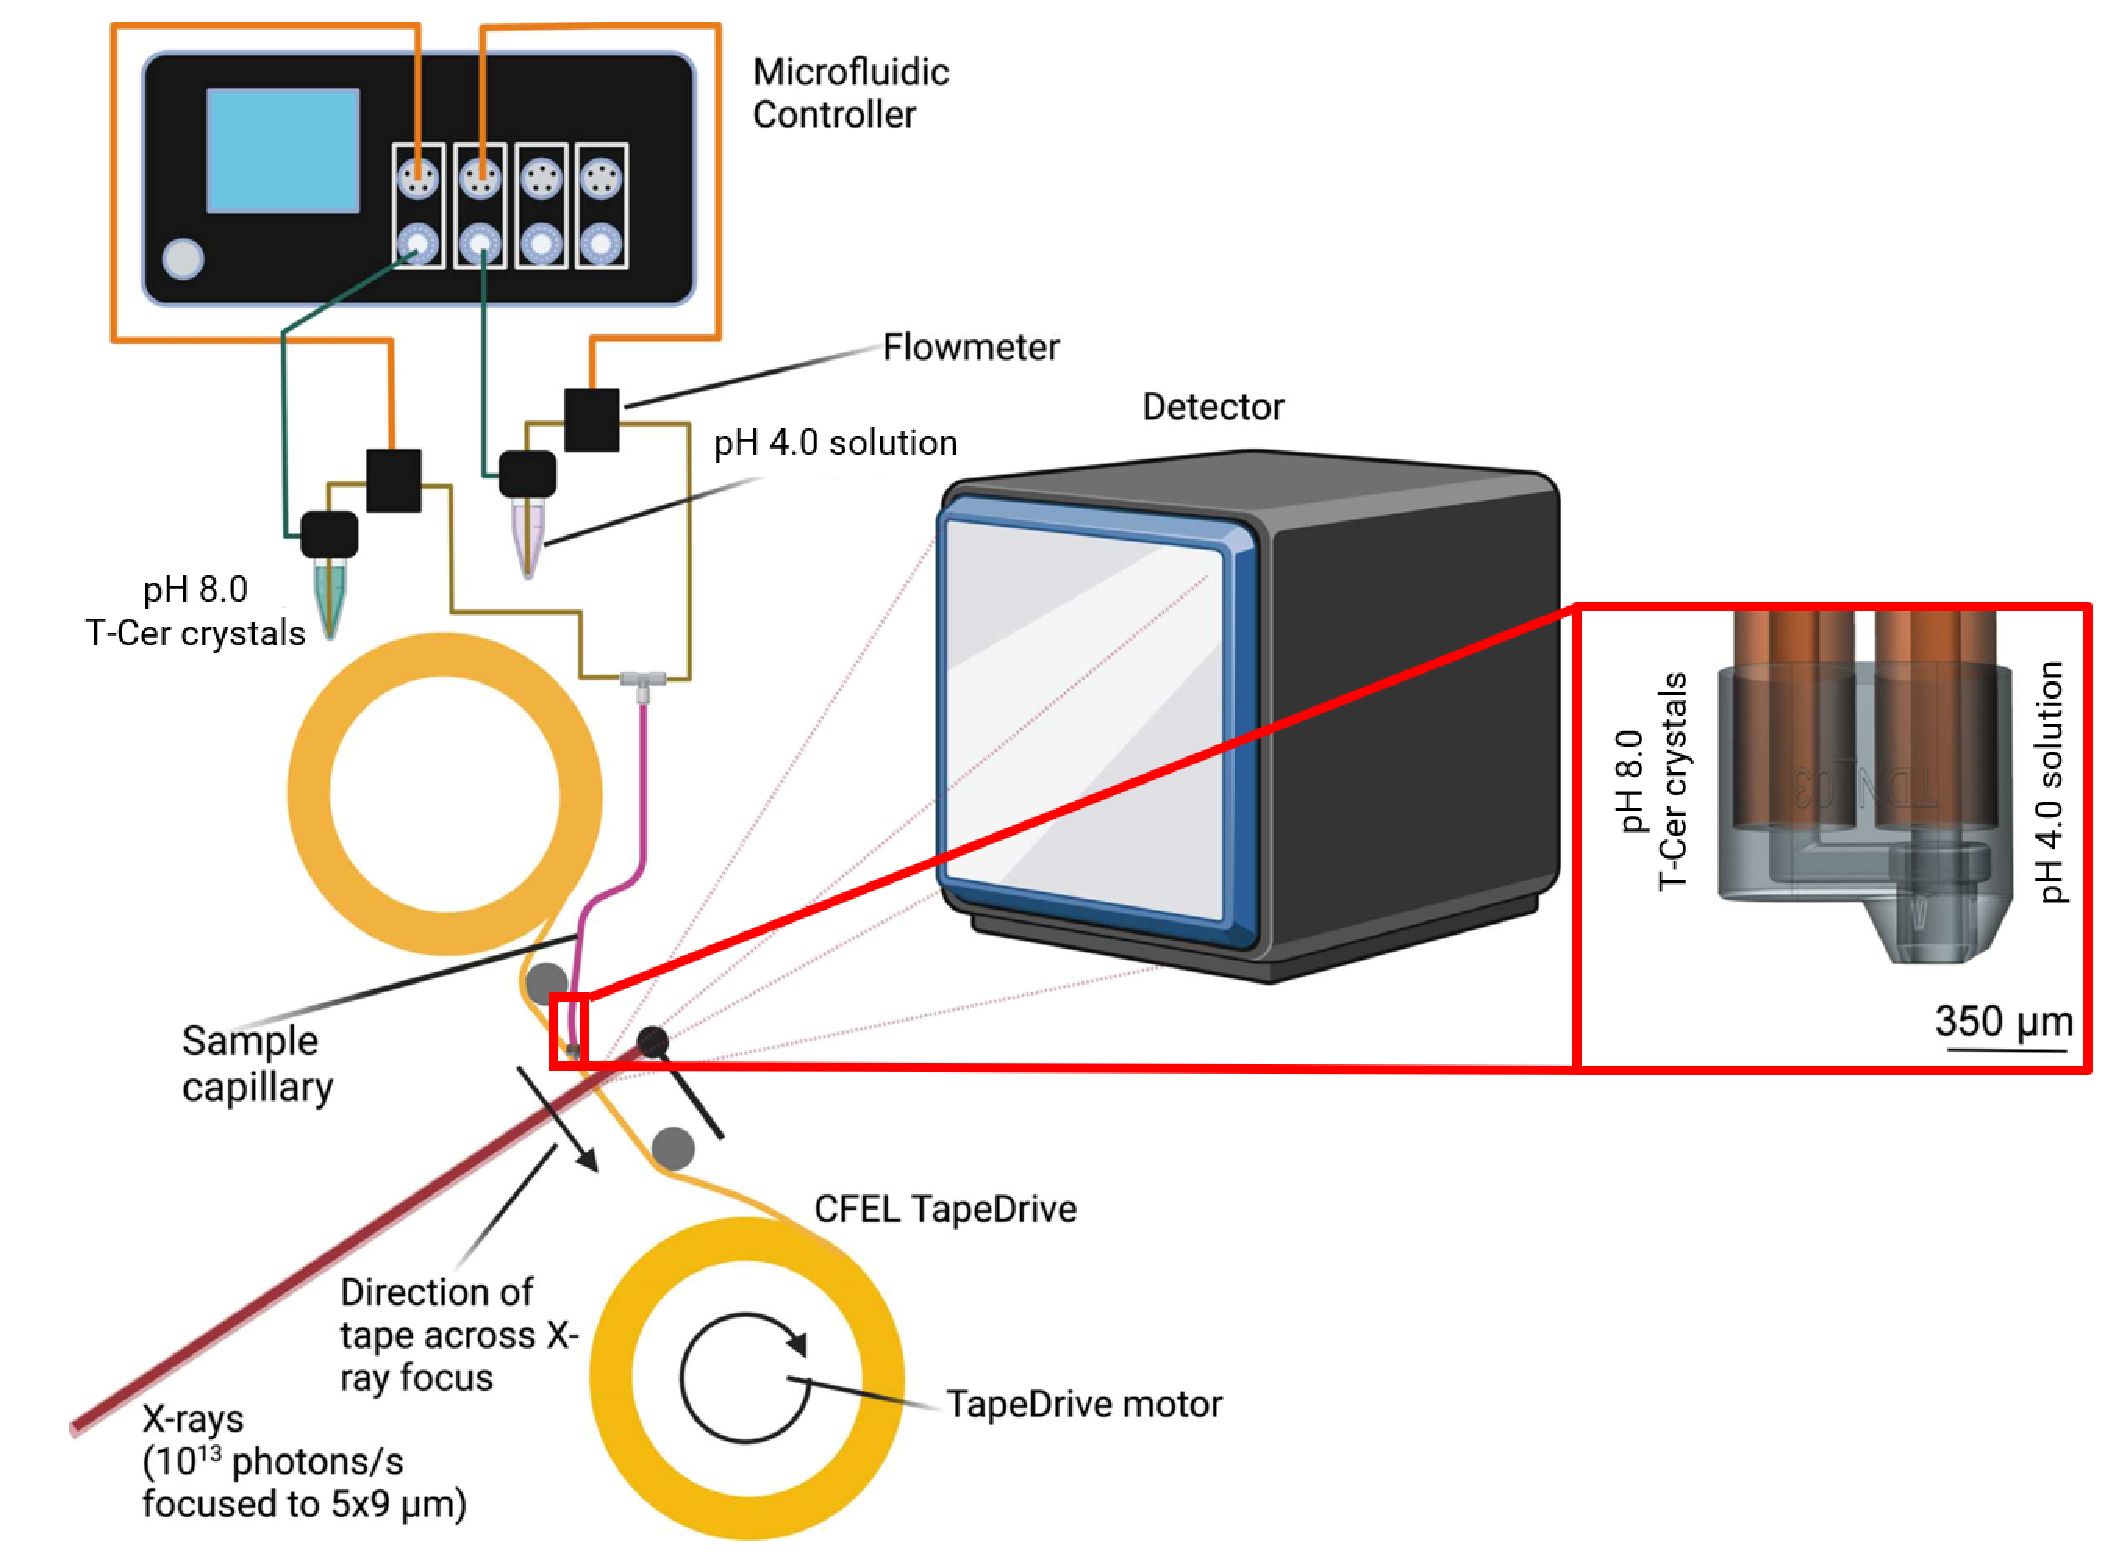
\includegraphics[width=\textwidth]{images/T-Cer/tape-drive_schematic.pdf}
    \hfill
    \caption{Schematic representation of the experiment planned at beamtime P11 (PETRA III). A first capillary (left) brings a slurry of microcrystals of T-Cer, suspended in pH 8.0 mother liquor to a fast-mixing nozzle. A second capillary flows pH 4.0 mother liquor (right). At the end of the nozzle, both flows meet, and the resulting mix is deposited on the tape. The end of the nozzle can be considered as t=0 (beginning of mixing). The delay between the beginning of the mixing and the X-ray exposure is determined by the speed of the tape and the distance between the nozzle position and the X-ray beam position. This delay constitutes the investigated time point. This figure is adapted from \cite{zielinskiRapidEfficientRoomtemperature2022} and \cite{henkelJINXEDJustTime2023}}
    \label{fig:tape drive}
\end{figure}

Compared to the anterior ‘mix-and-inject’ setups (see Section \ref{sec:diffusion}), the tape drive setup is considerably less sample intensive (meaning that a lower volume of crystal slurry is needed to collect the same amount of diffraction images). This is because viscous or liquid jetting devices require flowing the sample at a relatively high speed to ensure stable jets (of note, this issue is considerably more pronounced for liquid jets). 

During the first experiment, happening in June 2021, the suspension of T-Cer microcrystals at neutral pH was mixed with an acidic pH mother liquor (same proportion of PEG and MgCl\textsubscript{2}, and 100 mM of pH 4.0 sodium citrate instead of pH 8.0 HEPES). This solution was chosen so that only the pH of the crystals would be affected by the mixing, and the concentration of every other molecule would be maintained. 

\subsubsection{Fixed-target setup coupled with LAMA on T-REXX}\label{sec:LAMA}

Before the second tape drive experiment on P11, two TR-SSX beamtimes were organised on beamline P14-2 (T-REXX) operated by the EMBL Hamburg.  T-REXX is the secondary hutch of beamline P14, where the X-ray beam is further focused to 10 \textmu m, with a flux of \(10^{12}\) photons/s. The beam on T-REXX is continuous (the beam is produced by a synchrotron source \footnote{Synchrotrons can be considered pulsed to some extent given that photons are generated only when an electron passes through an undulator or a bending magnet. This property is at the core of pump-probe Laue crystallography experiments carried out in the early 2000' \parencite{srajerPhotolysisCarbonMonoxide1996, moffatLaueDiffractionTimeresolved2019}. For standard MX experiments and SSX experiments, synchrotron sources can reasonably be approximated as continuous.} and is not chopped to create pulses) As discussed previously, the T-REXX beamline was the first beamline ever designed specifically for TR-SSX experiments (see Section \ref{sec:existingfacilities}), and has been at the forefront of TR-SSX development ever since.  

T-REXX and uses a fixed-target crystal delivery strategy with a robust sample environment \footnote{The beamline can be used and has been used with other sample delivery strategies. Nonetheless, the overwhelming majority of beamtimes are fixed-target experiments, and this standardisation is part of the beamline's strength.} combining humidity control, ligand dispensal and a unique collection scheme. Microcrystals of protein are pipetted on silicon nitride etched chips, containing wells \parencite{muellerFixedTargetMatrix2015}. Excess mother-liquor is sucked by a vacuum pump, bringing the crystals in the wells (full loading protocol is detailed in \cite{schulzHitandreturnSystemEnables2018}). The loaded chip is then mounted on the beamline, where the entire sample environment is contained in a humidity chamber to ensure a homogeneous level of hydration for all crystals of the chip (the sample environment utilised at T-REXX is schematised in Fig. \ref{fig:T-Cer_TREXX}). Picoliter droplets of ligands - 1M Sodium Acetate at pH 4.0 for this beamtime - can be dispensed right on one of the wells etched onto the chip using the LAMA method \parencite{mehrabiLiquidApplicationMethod2019}, before the sample present into that well is exposed to the X-ray beam. This is the second approach outlined in Section \ref{sec:presenting_tpd_P11}, it maximises the ligand/crystal ratio since the crystals have previously been isolated from their mother liquor. During data collection, a crystal is first shot by the picoliter liquid dispenser and brought to the X-ray beam after a set delay via a raster movement (schematised as a blue trace in Fig. \ref{fig:T-Cer_TREXX}). A single fixed-target chip has upwards of 20,000 wells; for a delay of 1s, shooting and then exposing all wells means a minimal collection time of more than five hours. In order to circumvent this issue, the Hit-And-Return (HARE, \cite{schulzHitandreturnSystemEnables2018}) collection scheme was developed to interleave shooting and collection, significantly decreasing the time needed to collect a chip, down to \textasciitilde 20 min. In good conditions, a complete time point can be recorded under one hour. 

\begin{figure}[H] %bt!]
    \centering
        \noindent 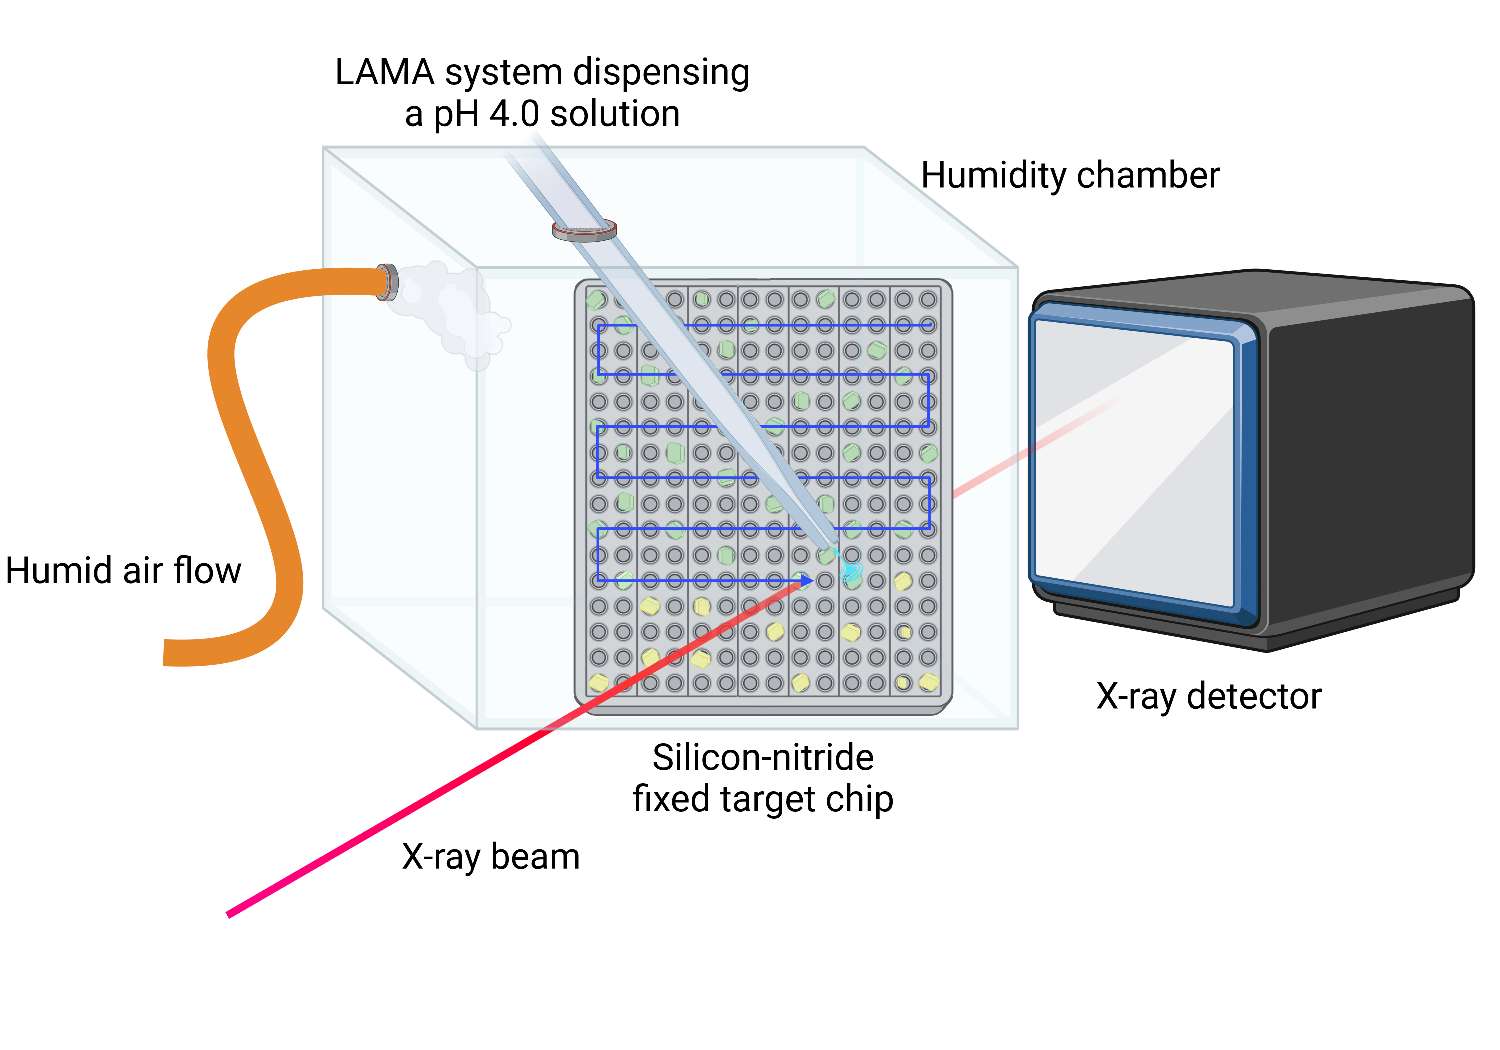
\includegraphics[width=\textwidth]{images/T-Cer/T-REXX_LAMA.pdf}
    \hfill
    \caption{Representation of the setup used on beamline P14-2 T-REXX. Microcrystals of T-Cer grown at neutral pH (yellow, in the figure) are loaded on silicon nitride HARE chips using the protocol described in \cite{mehrabiHAREChipEfficient2020}. The crystals are maintained in a humid atmosphere during loading, mounting and data collection to preserve them at room temperature. The chip is translated into the beam so that every other row is scanned (blue trajectory) to avoid cross-contamination of the wells. For each well, a nanoliter droplet of 1M pH 4.0 Sodium Acetate (schematised as a blue droplet in the figure) is first deposited using the LAMA system (\cite{mehrabiLiquidApplicationMethod2019}, schematised by the elongated pipette in the figure), inducing a pH drop in the crystals (schematized as a colour change from yellow to green in the figure). After a set delay, the crystal is exposed to the X-ray beam (red in the figure) for diffraction data collection.}\label{fig:T-Cer_TREXX}
\end{figure}

The resolution of the reference dataset (REF-LAMA, containing 30 000 indexed patterns) is 1.7 \AA, better than that of the dataset collected on P11 (REF-TPD-1). This suggests that the resolution of the datasets collected on P11 previously was limited by the detector position, not by the diffraction capabilities of T-Cer micro-crystals.

\subsubsection{Characteristics of beamline ID29}\label{sec:presenting_ID29}

Beamline ID29 was one of the main beamline refactoring projects happening within the frame of the Extremely Brilliant Source (EBS) upgrade plan of the ESRF, making the ESRF the first fourth-generation synchrotron source. ID29 was built with serial crystallography in mind, with the aim to maximise the increased flux available after the EBS upgrade.

The post-EBS storage ring produces a beam that is \(10^2\) times more brilliant than it was before the upgrade \parencite{griecoStructuralDynamicsFunctional2024}. The horizontal emittance of the storage ring was also greatly reduced, producing a more focused beam with a circular cross-section (Fig. \ref{fig:ID29_beamline} (a)). ID29 uses a multi-layer monochromator, producing a 1 \% bandwidth beam, with the consequence of increasing photon flux since fewer photons emitted by the electrons passing through the undulator are filtered out. Combined, these two upgrades bring the photon flux of ID29 into the range of \( 10^{15}\) photons/s. 

This drastically increased photon flux allows for decreased X-ray exposure time for the collection of a diffraction frame while maintaining the signal/noise ratio. To produce such short exposure times, the beam of ID29 is chopped into pulses. The beamline uses a primary chopper (Fig. \ref{fig:ID29_beamline} (c)), consisting of a disk, pierced with slits on its diameter, aligned parallel to the beam and rotating at high speed. X-rays are transmitted only when the slits are aligned with the beam path. An important benefit of this chopper is to decrease the heat load downstream: the beam is only shone on the optics during the pulse. When operated at 231.25 Hz, its standard speed, this chopper produces pulses of 90 \textmu s (Fig. \ref{fig:ID29_beamline} (f)). This chopper defines the repetition rate of the beamline. By changing the speed of the chopper and spacing between the slits (two sides of the chopper are visible in Fig. \ref{fig:ID29_beamline} (d), with different spacings between the slits), the repetition rate of the beamline can be increased 925 Hz. 
\noindent The beamline also uses a secondary chopper (Fig. \ref{fig:ID29_beamline} (e)), consisting in a disk aligned perpendicular to the path of the X-ray beam, and pierced with a unique hole is used to further decrease the duration of the X-ray pulse if needed. When both choppers are used, the duration of an X-ray pulse can be decreased to 10 \textmu s (Fig. \ref{fig:ID29_beamline} (f)). The pulse sequence of ID29 is defined by the orbital clock of electrons in the storage ring (meaning it takes its phase is synchronised with the filling of the ring, and its base frequency is 925 kHz, a multiple of the orbital frequency of the bunches). The clock is replicated by two CITY modules: one for the choppers and a second one near the diffractometer. The sequence of events for data collection is propagated from that second CITY module to the instruments of the beamline (diffractometer, X-ray detector, \textit{ect}) by the SSXbox.

Because the beam of ID29 has a 1\% bandwidth, the Ewald sphere it projects on the reciprocal lattice of protein crystals has a 'thicker' surface (Fig. \ref{fig:ID29_beamline} (b) (see Section \ref{sec:dataprocan} for a more detailed explanation of the relation between wavelength, bandwidth, and the shape of the Ewald sphere surface). Because of this, reciprocal lattice points can be slightly or fully encompassed by the surface of the Ewald sphere (Fig. \ref{fig:ID29_beamline} (b)), and reflection will be slightly integrated over wavelength, increasing the size, intensity, and slightly elongating the diffraction spots (Fig. \ref{fig:ID29_beamline} (c)). This increased intensity and size of the diffraction spots should theoretically help with the indexing of still diffraction images, and the reflections produced with a 1\% beam contain information from a more complete Bragg peak, which should theoretically decrease the amount of indexed pattern needed for a full dataset (See Section \ref{sec:dataprocan} for the difference between using still SX diffraction images and standard rotation MX diffraction images).

\begin{figure}[H] 
    \centering
        \noindent 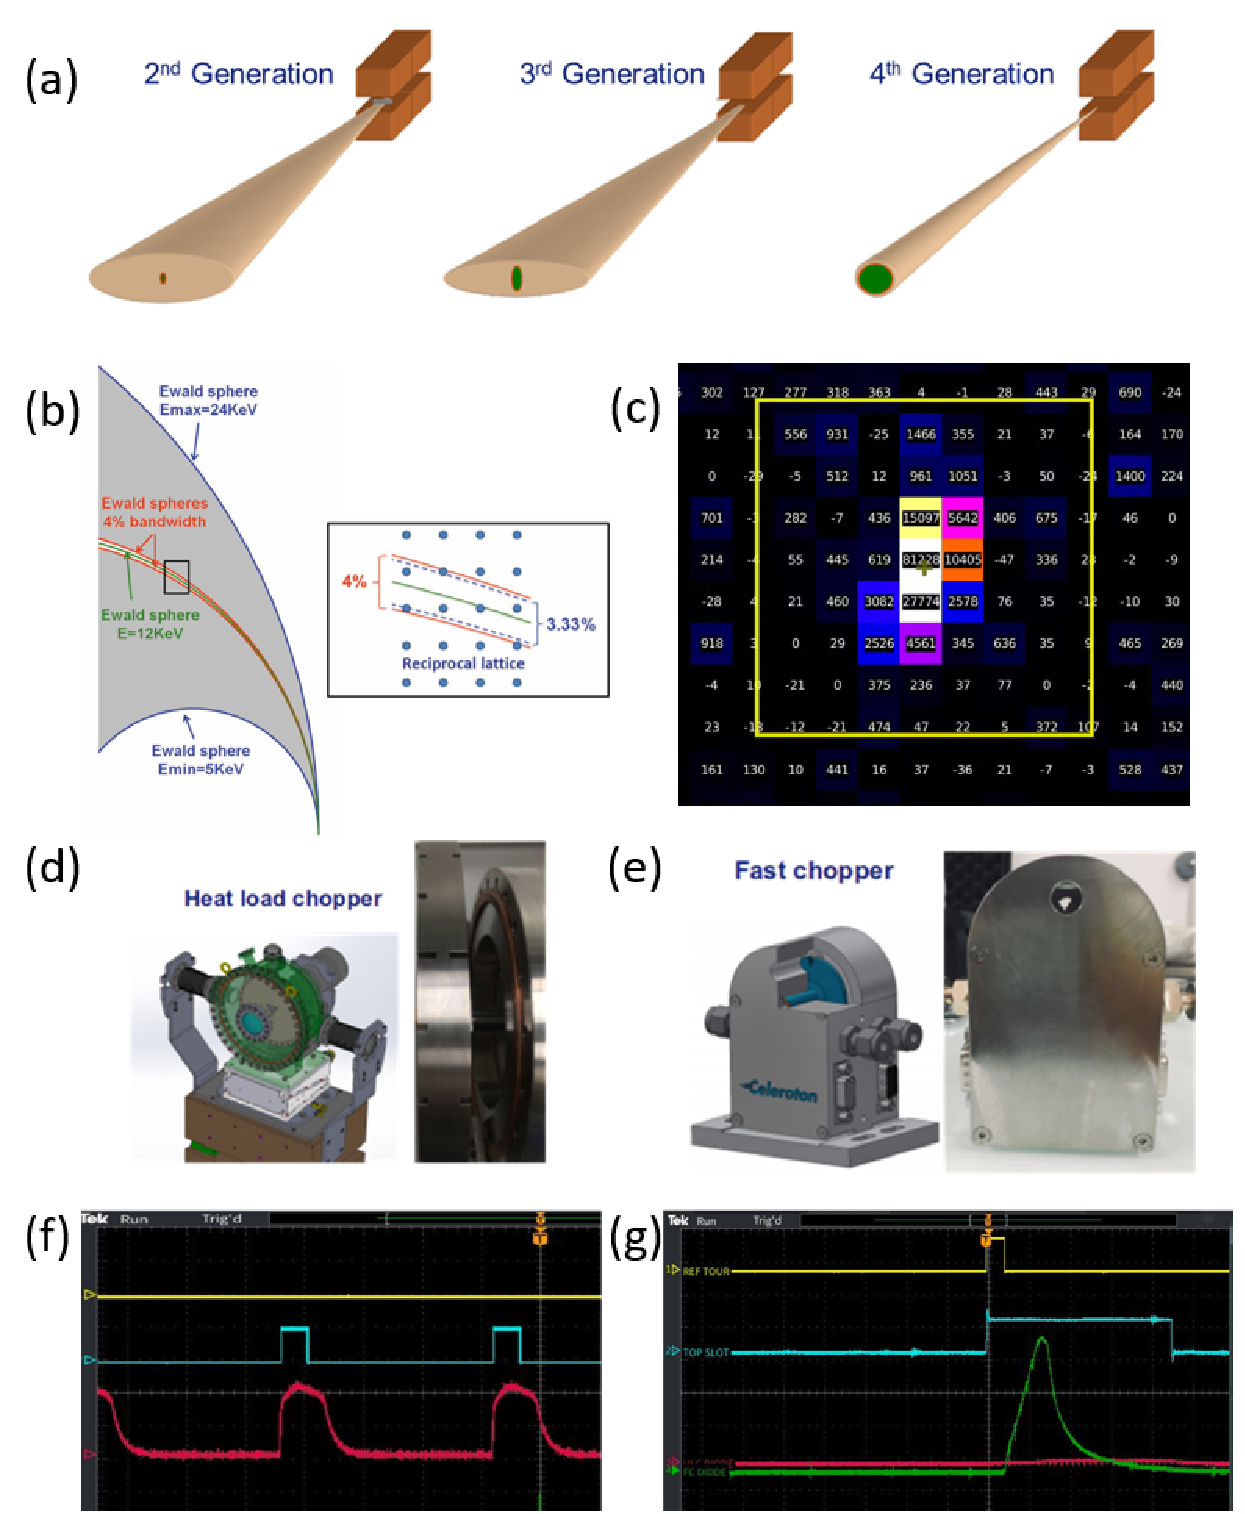
\includegraphics[width=0.8\textwidth]{images/T-Cer/ID29_beamline.pdf}
    \caption{Technical upgrades making the ID29 beamline. (a) Schematic representation of the image of the X-ray beam after an undulator for 2nd, 3rd and 4th generation synchrotron. After the Extremely Brilliant Source upgrade, bringing the ESRF to the 4th generation synchrotron, the tail of the beam (beige coloured) is no longer horizontally elongated. As a consequence, the X-ray beam after the undulator has a tighter cross-section. (b) Schematic representation of the consequence of using a slightly poly-chromatic X-ray beam on the Ewald sphere for X-ray crystallography. Standard MX beamlines have a negligible bandwidth (green trace), ID29 has a 1 \% bandwidth, which increases the cross-section of the Ewald sphere and allows reflections from reciprocal lattice points to be more fully integrated (red trace) (reproduced from \cite{dejoieUsingNonmonochromaticMicrobeam2013}, importantly, in this figure, the bandwidth is of 4 \%, that of ID29 is of 1\%) (c) Diffraction spot from an image collected on ID29, exhibiting an elongated shape as the reflection in integrated over wavelength. (d) The primary X-ray beam chopper, consisting of a slitted disc (green, first panel) rotating at high speed, aligned parallel to the beam path (black tube, first panel). The X-ray beam passes through the black tube in the first panel and is only transmitted when the beam is aligned with one of the slits visible on the second panel. This chopper defines the base frequency of the beamline and decreases the heat load by cutting the continuous beam of the synchrotron into usable pulses.  (e) The secondary chopper, consisting of a disc pierced with a unique hole, rotates at high speed and is positioned perpendicular to the X-ray beam. The X-rays are only transmitted when one of the holes is aligned with the beam path,  creating a shorter pulse. The hole has a scaled pyramid shape, meaning that by adjusting the height of the secondary chopper, the width of the hole -and therefore the duration of the X-ray pulse - can be changed from 10 to 20 or 30 \textmu s. (f) Pulse sequence of ID29 when only the primary chopper is used, the readout from the X-ray diode is plotted in red, and blue is the TTL signal to the detector from the CITY module. (g) Pulse sequence of ID29 when both choppers are used, the readout from the X-ray diode is plotted in green, and blue is the TTL signal to the detector from the CITY module. The X-ray pulse is 10 \textmu s long}\label{fig:ID29_beamline}
\end{figure}
ID29 produces intense \textmu s long X-ray pulses, which are slightly integrated over wavelength. It is the only synchrotron beamline capable of achieving a time resolution in the range of the \textmu s for TR-SSX at the moment \footnote{TR-SSX excludes techniques such as TR-Laue crystallography, which can achieve ps time resolution \parencite{moffatLaueDiffractionTimeresolved2019}, and Hadamard Transform TR-MX \parencite{yorkeTimeresolvedCrystallographyUsing2014}. Further, a beamline is currently being built with the same design as ID29 at the MAX VI synchrotron source in Lund, Sweden. It was, at the time of writing this manuscript, not yet operating.}. It is, therefore, uniquely suited for TR-SSX experiments.
\begin{table}
    \centering
    \begin{tabular}{|c|c|} \hline 
         Energy& 11 - 15 keV\\ \hline 
         Bandwidth& 0.4\% and 1\% (\textdelta E/E)\\ \hline 
         Flux& \(\sim 3 \times 10^{15}\) photons/s\\ \hline 
         Beamsize& \(4 \times 2 \mu m ^2\)\\ \hline 
         Beam divergence& \(1.9 \times 0.7\) mrad\\ \hline 
         Exposure time (fast chopper and heat-load chopper)& 10 - 20 - 30 \textmu s\\ \hline 
         Exposure time (heat-load chopper)& 90 \textmu s\\ \hline 
         Repetition rate& 231.25 hz\\ \hline
    \end{tabular}
    \caption{Capabilities of the beamline ID29}
    \label{tab:ID29_stats}
\end{table}

\subsubsection{The Lübeck tape drive}\label{sec:lubeck}

In September 2022, the commissioning of beamline ID29 started. T-Cer-s (construct described in Section \ref{sec:short}) was proposed as a target to test the TR-SSX capabilities of the beamline using a novel tape drive setup, as part of an ongoing collaboration with the group of Manfred Roessle in Lubeck. This was the first genuine TR-MX experiment of the beamline. That beamtime aimed to repeat the protocol carried out at P11 (Section \ref{sec:presenting_tpd_P11} and \ref{sec:P11-2}), with improvements made to the construct (will be discussed, later, in Section \ref{sec:short}) and to the crystallisation condition (will be discussed, later, in Section \ref{sec:ammonium}). Unfortunately, it turned out the version of the setup used at the time could not accommodate crystal suspensions in which mother liquor was under a certain degree of viscosity. The less viscous crystallisation condition engineered to shorten mixing and diffusion times was also more prone to micro-crystal settling. As the crystal settled, clumps formed which rendered the crystal flow non-continuous and caused clogging in the sample capillaries. Therefore, the decision was taken during the beamtime to switch back to the sample used for the P11 and T-REXX beamtimes, which could crystallise overnight. A dataset was recorded using proteolysed T-Cer crystals grown in PEG to complete the data recorded on P11 (Section \ref{sec:P11-2}). 

The tape drive setup used for this experiment on ID29 was developed by the team of Manfred Rößle at the Technical Applied University of Lübeck (TH Lübeck, Germany). Contrary to the P11 tape drive, it is positioned horizontally, with the tape flowing from top to bottom (Fig. \ref{fig:ID29_tpd} (a)). This tape drive setup also features a secondary blotting tape, made of cellulose, designed to suck the excess liquid around the crystal once they have been deposited on the sample tape (Fig. \ref{fig:ID29_tpd} (a)), reducing X-ray scattering by the liquid and therefore the backreference on diffraction images. This improves data quality (Lahey-Rudolph \textit{et al.}, in preparation). 

Prior to being brought to the tape by Teflon capillaries (Fig. \ref{fig:ID29_tpd} (b)), the sample is stored in Hamilton syringes. The flow of the sample is controlled by the force exerted on the syringe, determined by a paced motor. In order to limit the settling of the crystal due to gravity, the syringe oscillates 90 \degree. 

The setup designed by the Lübeck team was intended for the study of light-activated reactions, using a light source as the pump of the pump-probe experimental scheme. To make it compatible with mixing TR-MX experiments, we added a T-junction to the sample capillary (Fig. \ref{fig:ID29_tpd} (b)). Upstream of this T-junction, a new capillary brings a pH 4.0 buffer, mixing it with the sample to initiate the pH drop. The flow of the pH buffer capillary was maintained higher than that of the crystal capillary to ensure that mixing would produce a pH 4.0 environment. The delay between mixing and X-ray exposure could be adjusted by changing the flow in each capillary. Importantly, this setup can only probe long delays (>30 s) after mixing.
\begin{figure}[H] 
    \centering
        \noindent 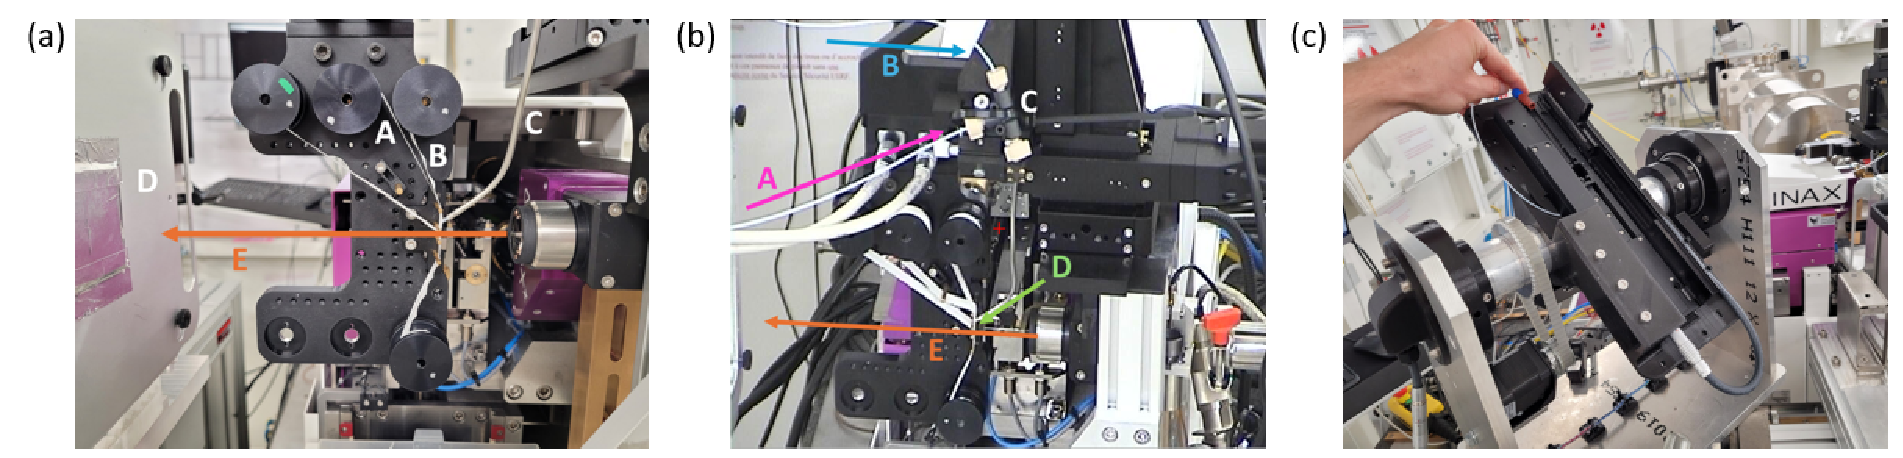
\includegraphics[width=\textwidth]{images/T-Cer/ID29_tape-drive.pdf}
    \caption{tape drive setup of the ESRF. (a) Overview of the sample environment, taken perpendicular to the X-ray beam path (E, orange). The tape drive scaffold is visible in black in the background of the image. In addition to the P11 setup, a secondary blotting tape made of cellulose (A) grazes the tape on which the sample is deposited, made of pierced mylar (B) from behind to remove excess liquid. The small holes in the sample tape allow liquid to be sucked away by capillarity. The sample is brought by a Teflon capillary guided in a metal sleeve (C). X-ray diffraction images can be collected with high acquisition rates using the Jungfrau detector (D). (b) The setup was used to record the dataset 60 seconds after mixing. pH 4.0 buffer is brought by a Teflon capillary (A)  Neutral pH T-Cer crystals are brought from a Hamilton syringe in a second capillary (B). Both capillaries are plugged into a T-junction (C), and the mixed sample is brought to the sample tape by the outgoing Teflon capillary (D). The flow in capillaries A and B can be adjusted to reach the desired time of travel between the T-junction and the point of exposure to the X-ray beam (E). (c) Anti-settling device: the Hamilton syringe containing microcrystals of T-Cer, plugged into capillary A, lies on a bed, oscillating between -45 \degree and 45 \degree to limit the settling of microcrystals by gravity, which can cause clumps of crystals and clogging of the capillaries.}\label{fig:ID29_tpd}
\end{figure}
At neutral pH, in their reference state, the micro-crystals of T-Cer produced overnight diffracted to 2.2 \AA\ resolution (Fig. \ref{fig:ID29_results} (a)). While the edge of the detector was set at 2f.0 \AA, the lower resolution of this reference state structure compared to that collected on T-REXX and P11 is very likely linked to the limited size of the sample, as a result of the short time between setting up the crystallisation batch and data collection. All amino acids in the chromophore pocket are in their neutral pH conformation (Fig. \ref{fig:ID29_results} (a)). 

\subsubsection{The acoustic levitation device}\label{sec:ALD}

Briefly, the ALD setup deployed on beamline PXI X06SA at the Swiss Light Source (SLS) \parencite{tsujinoUltrasonicAcousticLevitation2016, kepaAcousticLevitationRotation2022} relies on maintaining a droplet containing crystals in the beam focal point at constant rotation. A picoliter liquid dispenser is used to mix a ligand in the droplet, and diffraction data is acquired at a set delay after the mixing has begun. This setup utilises the \(\sim 100 \times 100 \) \textmu m\textsuperscript{3} configuration of the beam. Therefore, it requires large crystals. Because the droplet can be maintained in place for an extended duration, this setup is able to investigate longer delays than the tape drive and fixed targets used previously, and thus is particularly suited for the study of the pH drop-induced isomerization of T-Cer's chromophore. 

The flux on beamline PXI X06SA is weaker than that of the ESRF beamlines (\(10^{12}\) photons/s). While a disadvantage for standard cryogenic temperature MX data collections, this is less relevant for RT-MX experiments, where the flux must be limited to collect data for extended periods without causing too much radiation damage. 

The acoustic levitation device (ALD) setup deployed on beamline PXI X06SA (Fig. \ref{fig:T-Cer_ALD} (a,b)) relies in a large piezoelectric transducer (Langevin horn, marked with letter A in Fig. \ref{fig:T-Cer_ALD} (a)) producing an ultrasonic wave. It produces acoustic waves with a wavelength of \textasciitilde 9 mm (resonance frequency of \textasciitilde 38 kHz), and is facing a concave acoustic reflector (marked with letter 'B' in Fig. \ref{fig:T-Cer_ALD} (a)) \parencite{tsujinoUltrasonicAcousticLevitation2016}. When the distance between the piezoelectric transducer and the reflector is a multiple of half that wavelength, pressure nodes are created by the standing waves. The force of the acoustic radiation pressure in these nodes exceeds that of gravity, allowing objects loaded at this position to remain in levitation.  

When a crystal is sitting in a droplet levitated by acoustic pressure, acoustic streaming of air at the surface of the droplet causes it to rotate \parencite{zhaoInternalCirculationDrop1999}. This is ideal for a crystallography measurement as it will ensure that all orientations of the crystal(s) are presented to the X-ray beam. However, the rotation speed of a droplet in the acoustic radiation pressure node is difficult to estimate, and the rotation speed of a crystal trapped in the droplet might be different due to inner liquid currents in the droplet. In these conditions, estimating the 'oscillation range' of the crystal during the integration time of a diffraction frame is extremely challenging at best. 

To improve that aspect, Takashi Tomizaki and collaborators designed nanodisks with blades reminiscent of that of a helicopter \parencite{kepaAcousticLevitationRotation2022}. The nanodisks used for this beamtime (marked with the letter 'F' in Fig. \ref{fig:T-Cer_ALD} (b)) are made of polyimide foils, with a diameter of 4 mm, and four tiny blades (they correspond to the Type 2 disks described in \cite{kepaAcousticLevitationRotation2022}). By varying the difference between the static pressure at the centre and on the edge of the pressure node, the rotation speed of the disks can be adjusted from 20 rotations per second to less than one rotation per second. With such high rotation speed, collecting a complete dataset is extremely fast, provided the acquisition rate of the detector is high enough. This is why this setup utilises a Jungfrau 4M or an Eiger 1M, which can operate at 3 kHz. A small volume of mother liquor can be pipetted on the nanodisks.

However, because the droplet is larger than the crystals, crystals come and go in and out of the beam as the droplet rotates. Further, in order to ensure a high hit rate, several crystals are loaded in each levitating droplet, which inevitably leads to some images containing diffraction from two differently oriented crystal lattices. Therefore, the data collected with this setup are processed as SX data, and processed with the workflow detailed in Section \ref{sec:dataprocan}, except measured reflections were merged with the Monte-Carlo merging approach proposed in the process\_hkl tool, which performed better than \textit{partialator} for non-partial reflection measurement.

The ALD setup utilises nanolitres droplet dispensers (BioFluidix PipeJet nano dispenser) to mix ligands into the levitating drop containing crystals and initiate reactions in the protein crystals. The droplet dispensers are symmetrically mounted in opposing positions on each side of the levitation position (marked with the letter 'C' in Fig. \ref{fig:T-Cer_ALD} (a) and (b)). Both nanolitre dispensers are carefully aligned so that the force of the incoming nanolitre droplets (visible on the second panel of Fig. \ref{fig:T-Cer_ALD} (c)) 'cancel out', which prevents the levitating nanodisk from being knocked out of the pressure node by the impact of one droplet. The impact of both nanolitre droplets creates a strong convection movement in the levitating drop, as evidenced by its deformation visible in the third panel of Fig. \ref{fig:T-Cer_ALD} (c).

Thanks to this design, diffraction data can be collected while or directly after the levitating drop is shot by ligand droplets. Thanks to the high collection rate of the detectors, short time points in the ms time window can be achieved. 



\subsubsection{TR-MX experimental scheme with the ALD setup}\label{sec:ALD_protocol}

Mixing-probe delays were determined using a TTL pulse generator controlling both pH buffer dispensing and the initiation of the collection sequence of PXI (opening of the shutter and recording of diffraction images by the detector). The experimental sequence was designed to control the volume of pH buffer dispensed (by choosing the number of rapid sequential firing of each nanolitre dispenser), and the duration of the data collection was set to 1s. 

3-4 crystals of T-Cer-s were first pipetted onto a nanodisk, in a droplet of 3 \textmu l. The nanodisk was then manually mounted (with tweezers) into the middle acoustic radiation pressure node of the setup so that the droplet would be hanging under the levitating nanodisk (Fig. \ref{fig:T-Cer_ALD} (c)). Upon release from the tweezers, it immediately started to spin. The experimental hutch of PXI was then searched and locked. The nanodisk height had to be adjusted for the slight variation in the weight of the sample caused by the pipetting volume uncertainties. The intensity of the acoustic wave was slightly increased or decreased until the bottom of the levitating drop (where most crystals were) was on the beam position, using the high-speed camera (circled region on the screen in all panels of Fig. \ref{fig:T-Cer_ALD} (c) marks the beam position). Then the experimental sequence was manually started: 10 rapid shots of each nanolitre dispenser, then after a set delay, X-ray data collection for 5 s to limit radiation damage. In practice, most frames recorded more than 2 s after the opening of the X-ray shutter were discarded during data processing because the onset of global radiation damage limited their resolution.

\begin{figure}[H] %bt!]
    \centering
        \noindent 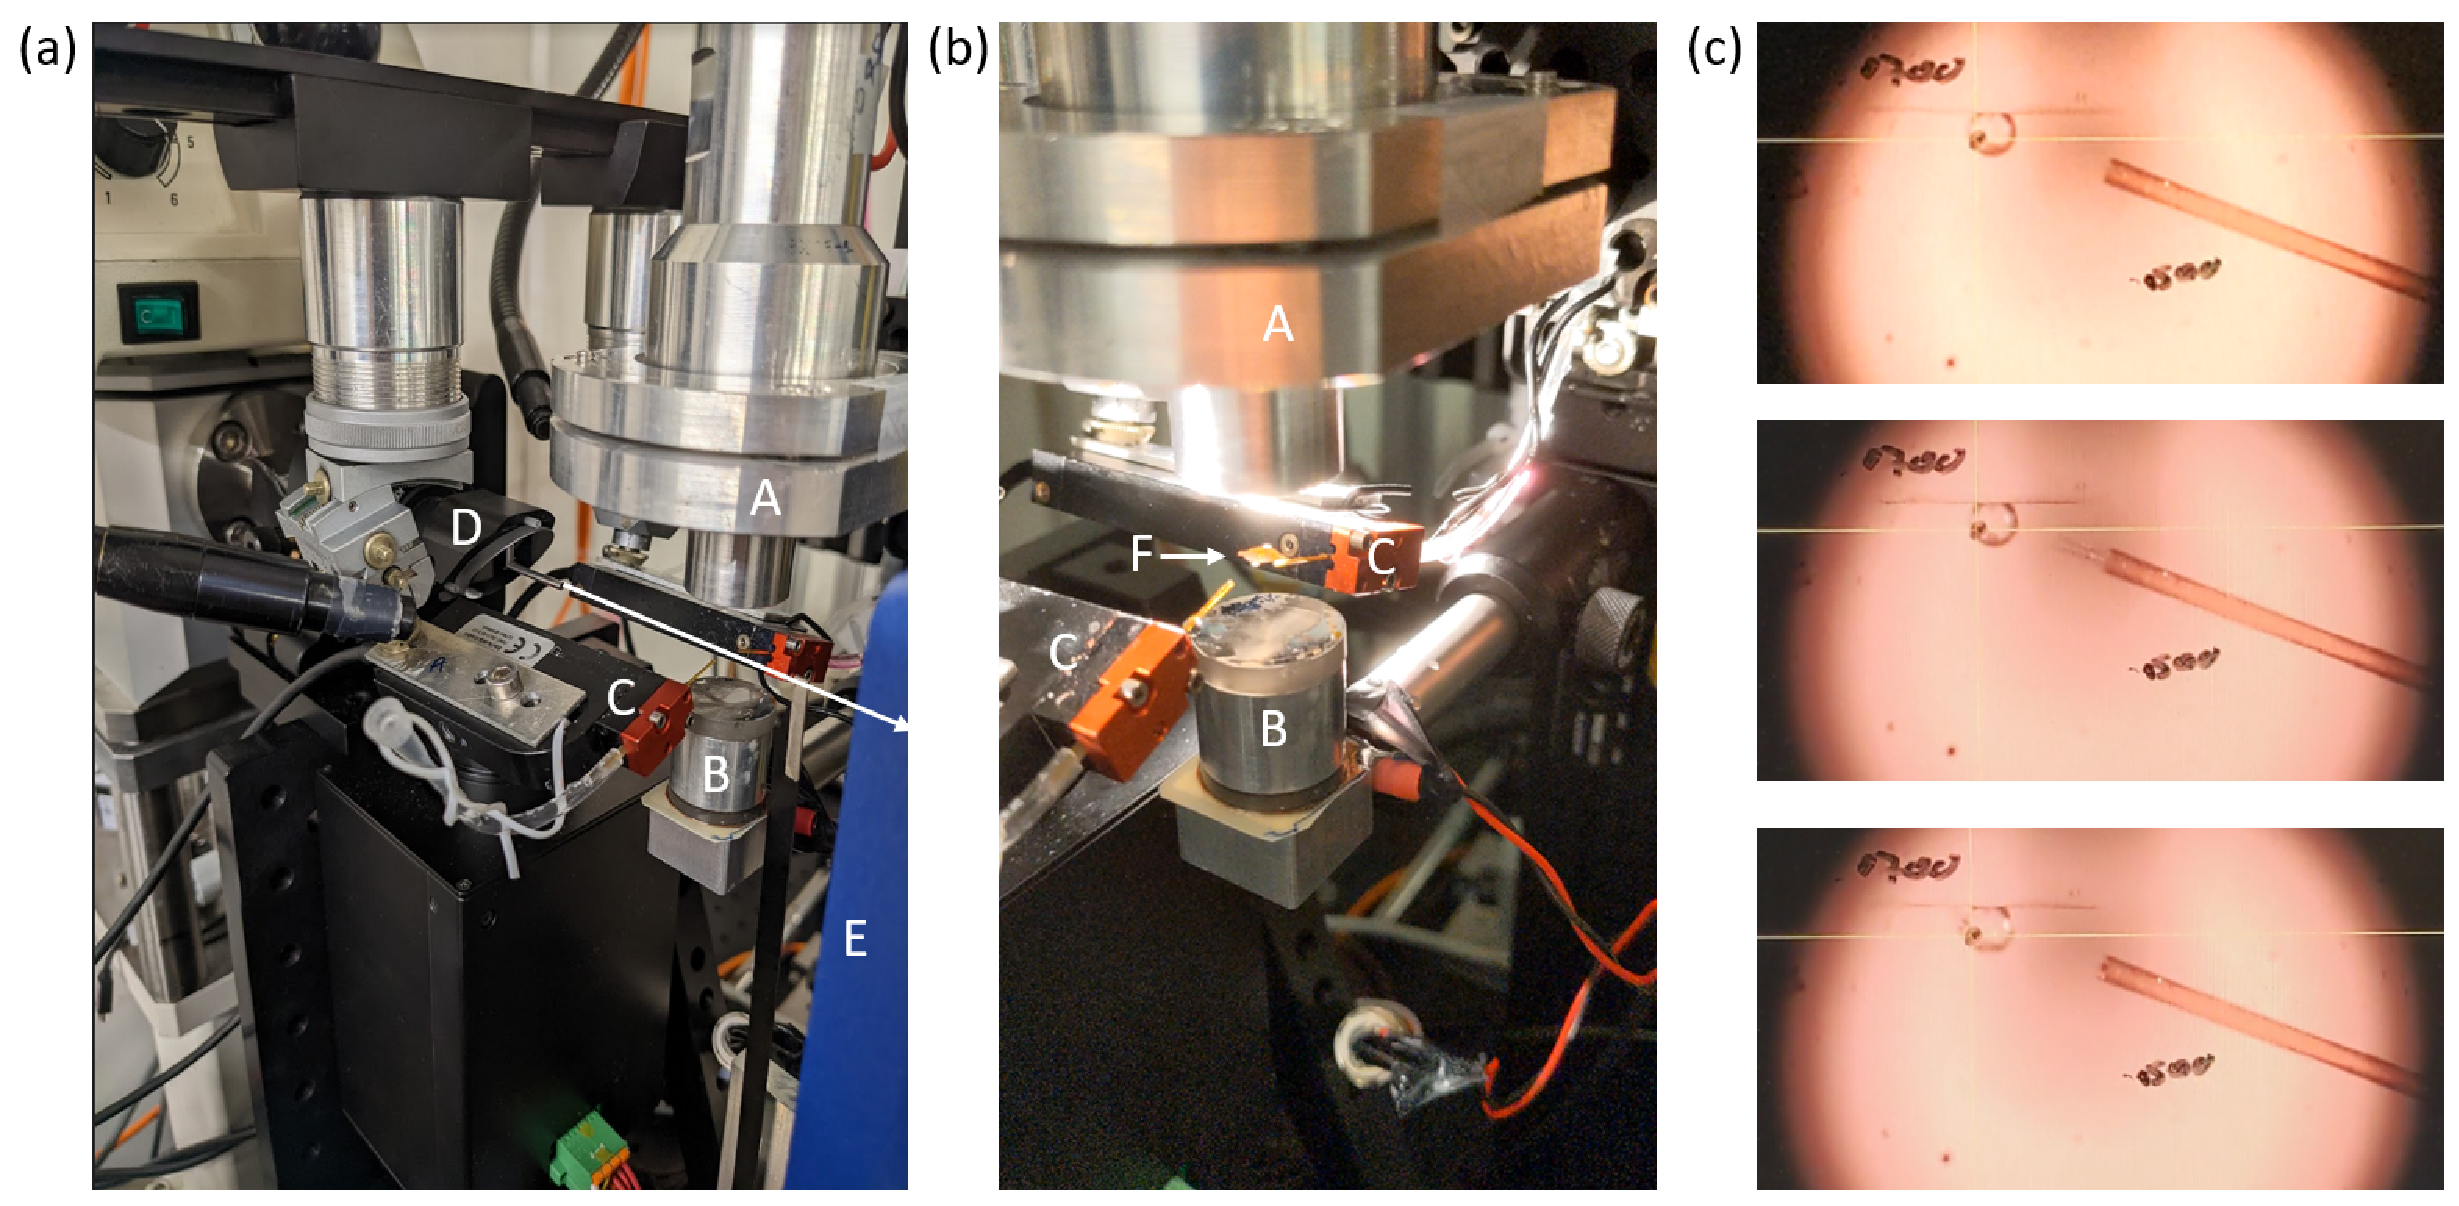
\includegraphics[width=\textwidth]{images/T-Cer/ALD_setup.pdf}
    \caption{Acoustic Levitation Device used on beamline PXI. (a) Overview of the setup from the detector side. A: Ultrasonic transducer; B: acoustic wave reflector; C: Picoliter dispenser (\textbf{REF}); D: X-ray capillary, the path of the X-ray beam is represented by a white arrow; E: Eiger 1 M detector. (b) close-up view of the setup, A-C same as in (a), F: nanodisk rotating in the standing wave zone. (c) Selected frames captured by the off-axis high-speed camera, showing the nanodisk rotating at the sample position (the droplet hanging from it contains T-Cer-s crystals), then the instant when the picoliter-sized droplet of pH buffer is ejected, and finally, the deformation of the crystal droplet on impact.  The droplet remains stable in the X-ray beam focal point, even during mixing with the picoliter droplets, thanks to the symmetrical positions of the liquid dispensers.}\label{fig:T-Cer_ALD}
\end{figure}

Importantly, the current iteration of the ALD setup does not provide a way to maintain the crystal's humidity, which effectively limits the delays achievable as the sample will eventually dry out.  

\subsection{Rotation X-ray data Processing and analysis}

All standard MX data presented in this chapter were recorded on the beamlines of the Structural Biology Group or on the CRG beamline BM07-FIP2 at the ESRF. Datasets were indexed with XDS \parencite{kabschXDS2010} and scaled with aimLESS \parencite{evansHowGoodAre2013} within the autoPROC environment from Global Phasing \parencite{vonrheinAdvancesAutomatedData2018}. 

\subsection{Serial Crystallography data processing}

All serial crystallography data were processed within the CrystFEL environnement \parencite{whiteCrystFELSoftwareSuite2012,whiteProcessingSerialCrystallography2019}. A workflow of data processing for serial crystallography is presented in the introduction of this thesis (Sec. \ref{sec:SX_intro}). The indexing step was carried out with xGandalf \parencite{gevorkovXGANDALFExtendedGradient2019}, TakeTwo and \parencite{ginnTakeTwoIndexingAlgorithm2016}, iMOSFLM \parencite{powellRossmannFourierAutoindexing1999} used in this order. Data recorded on the T-REXX (Section \ref{sec:T-REXX}) beamline were first processed using their auto-processing pipeline and then re-processed offline on the ESRF cluster using CrystFEL 0.10. As an example of serial crystallography data processing, a brief workflow of the steps used for this dataset will be given. Data recorded at the Swiss Light Source (Sec. \ref{sec:ALD_protocol}) was processed during the beamtime using the PSI resources, and then again at the ESRF. 

\subsection{Example of serial crystallography data processing}

In the following subsections, I will present an example of the procedure used to process new serial-crystallography data, using the example of the Tape-drive data collected in December 2021 (Sec. \ref{sec:P11-2}).

The CrystFEL software \parencite{whiteProcessingSerialCrystallography2019} consists of a wrapping for several tools used to process serial crystallography data starting from the image files, all the way to a set of merged structure factors (.mtz or .hkl file). Some of these tools are developed externally (mostly the indexing programs as well as some of the peak-finders), while others are part of the CrystFEL environnement.  The CrystFEL package also features a graphical interface, which is the most convenient way of inspecting images and setting parameters for each steps. However, the scaled-up processing of a sufficient number of images for a full serial crystallography dataset will require the use of a dedicated processing facility with multithreading capability. 

The most convenient way to load images in CrystFEL is to prepare a 'list file', where each line is the path to an image file (in the case where they were saved with the .cbf format):
\begin{verbatim}
/path/to/the/image/file_00001.cbf
/path/to/the/image/file_00002.cbf
/path/to/the/image/file_00003.cbf
...
\end{verbatim}
If the images are produced by modern Dectris detectors, they will be stored in .h5 files, and the list file should feature on each line the path to the .h5 file containing the frame, followed by the frame number:
\begin{verbatim}
/path/to/the/image/file_00000.h5 //0
/path/to/the/image/file_00000.h5 //1
/path/to/the/image/file_00000.h5 //2
...
/path/to/the/image/file_00001.h5 //0
/path/to/the/image/file_00001.h5 //1
...
\end{verbatim}

Along with the list of images, CrystFEL requires a geometry file (.geom), which contains information about the detector to sample distance, wavelength, orientation and positions of the different panels of the detectors, as well as the eventual regions of the detector which should be masked. Most of this information is usually filled in before the beamline by the beamline's staff; however, because of the more 'hands-on' nature of the SSX sample environments, the sample-detector distance might need to be re-estimated for each beamtime or run. The procedure used to refine that value will be described below. 

\subsubsection{Peak height and background estimation}

The first step to process serial crystallography data is to inspect the images to derive the parameters needed for peak-finding. Each combination of beamline/sample delivery setup and detector will produce images with a different intensity profile\footnote{The background level and peak level of the tape-drive experiment carried out on beamline P11 can be assessed in Fig. \ref{fig:CrystFEL_analysis} (b).}.

This information will be used by the peak-finding algorithm, which will detect areas of the detector that are likely diffraction Bragg peaks. Several algorithms are shipped with CrystFEL; the most robust algorithm and most used is Peakfinder8. It relies on the calculation of radial averages and comparing it to the local standard deviation and background level to determine whether a set of 'hot' pixels correspond to a bragg peak. This algorithm was initially implemented within the Cheetah serial crystallography analysis environment \parencite{bartyCheetahSoftwareHighthroughput2014}. Peakfinder8 requires a rough estimate of the ratio between the average background level and the level of the strongest Bragg peaks, the number of 'hot pixels' by Bragg peaks. It is often useful to limit the maximal and minimal resolution at which peak search is performed. This will avoid diffusion based artefacts around the center of the diffraction frames and limit the number of diffraction peaks to make the indexing step faster. 

\begin{figure}[H] 
    \centering
        \noindent 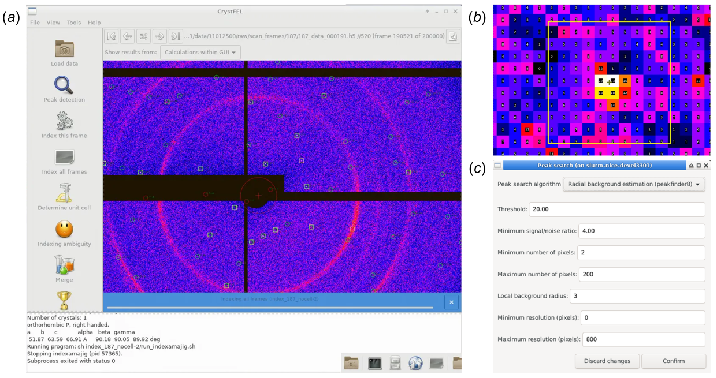
\includegraphics[width=\textwidth]{images/T-Cer/CrystFEL_peak.pdf}
    \caption{(a) Interface of CrystFEL 0.9, as available on the ESRF clusters at the time of data-processing. The diffraction frame showed was collected on P11. (b) Close-up view of a bragg peak, correctly picked up by the peak-finder, colour code corresponds to the photon count, written on the pixels. (c) peak-finder settings of PeakFinder8 used for this frame.}\label{fig:CrystFEL_analysis}
\end{figure}



Once the peak-finder settings (Fig. \ref{fig:CrystFEL_analysis} (c)) are set and tested on 10-20 frames to ensure that they are robust, indexing of all frames can proceed. 


\subsubsection{Indexing: Lattice parameters and geometry refinement}



Peak-finding, indexing and integration can be carried out for all frames at once using the \texttt{indexamajig} command, shipped with CrystFEL (Fig. \ref{fig:CrystFEL_analysis} (a)). The indexing procedure for still images is described in Sec. \ref{sec:SX_intro}. In it, the peak-finding algorithm, as well as its settings and the indexing algorithm(s) can be specified as follows: 

\begin{verbatim}
    indexamajig -i frames_1_999.lst
                -p T-Cer_ground-state_UC.cell
                -g T-Cer.geom
                -o ${j}_${n}.stream
                -j 16
                --peaks=peakfinder8
                --threshold=4
                --min-snr=4
                --int-radius=2,3,4
                --min-peaks 3
                --indexing=xgandalf-latt-cell,dirax-latt-cell,mosflm-latt-cell
                --xgandalf-fast-execution
                --multi
\end{verbatim}

The indexing algorithms use the peak list drafted for each frame potentially containing diffraction (hit-list) to determine the crystal lattice type and orientation if possible, leading to a set of "indexed lattices" (of which more than one can be detected on a given frame, if the \texttt{- -multi} flag is passed). The indexing algorithms can operate on prior knowledge of the lattice type and lattice parameters, but for a first round of indexing where geometry must be refined, it is often useful to run the indexing step first without prior knowledge. 

Since the indexing step is the most time-consuming, it is often wise to run the \texttt{indexamajig} command for packets of frames of 1000's or more so that more tasks can be filed at once to the cluster. \texttt{indexamajig} stores all found hits and indexing solutions, as well as integration results in a text-based file called a 'stream file', which can weigh up to several tens of gb. The files produced by different runs of \texttt{indexamajig} can be concatenated to produce a file containing all indexed frames. This stream file can be analysed first with the \texttt{cell\char`_explorer} function shipped with CrystFEL, which produces a histogram of all lattice parameters for indexed lattices, which can be further segregated into solutions. This histogram, as well as the 'indexing rate' (\% of lattices indexed over the number of images), is used to assess the quality of the indexing job. 

In order to assess the detector-sample distance (\texttt{clen}, for \textit{camera length} in the geometry file) in the tape-drive experiment, the indexing step is run with increasing values of detector-sample distance. The sample-detector distance value for which the histogram is the most centred on the expected values and distribution of the parameters are most Gaussian-shaped, as well as giving the highest number of correctly indexed lattices is the correct sample-detector distance. 

This method of geometry refinement is now deprecated, as newer versions of CrystFEL come with the \texttt{- -geopti} flag in the \texttt{indexamajig} command, which performs the geometry refinement simultaneously with the indexing, using a millipede approach. 

Once the detector-sample distance is refined satisfyingly and the layout and orientation of the detector pannel have been validated, \texttt{cell\char`_explorer} can be used to draft 

The integration step is performed for all frames after indexing, however, the partialities of each observation of a reflection as well as the lattice parameters for all indexed frames, must be refined. This is performed during the merging step.

\subsubsection{Merging: defining the resolution cutoff}

Merging data in CrystFEL is almost exclusively performed with \texttt{partialator}, a tool performing partiality correction and scaling before merging. The partiality correction accounts for the relative differences in intensity for a reflection based on the different orientations \parencite{ginnRevisedPartialityModel2015}. For the tape-drive data collected on beamline P11, partialator ran as below:

\begin{verbatim}
    partialator -i my.stream
                -o merged.hkl 
                -y 222 
                --max-adu=7000  
                --model=xsphere 
                --iterations=3
                --push-res=0.6
\end{verbatim}

The default behaviour of partialator is to enforce a resolution cutoff for each frame, the \texttt{- -push-res} flag is here to ensure that the cutoff enforced corresponds \texttt{0.6} nm\textsuperscript{-1} over the detected resolution limit for each crystal. This value is determined by comparing the data quality while increasing the \texttt{- -push-res} value and selecting the value yielding the best data quality. 

The figure of merit for each run of partialator can be calculated with the \texttt{check\char`_hkl} command as described below:

\begin{verbatim}
    check_hkl -i my.stream 
                -p T-Cer.cell
                --highres=2.1
\end{verbatim}

\texttt{check\char`_hkl} calculates Rsplit, (\(CC_{1/2}\) and \(CC^\ast\) for each resolution shell. The determination of the resolution cutoff for the set of structure factors produced by a given run of \texttt{partialator} involves running \texttt{check\char`_hkl} with increasingly lower \texttt{- -highres} values until a threshold of 35 \% of \(CC^\ast\) is met for the highest resolution shell. 

\subsubsection{Processing facilities used}

Data recorded at P11 (Section \ref{sec:P11_1} and \ref{sec:P11-2}) were processed on the MaxVI cluster, using their installation of CrystFEL 0.9, with contribution by the Oberthür group (Centre for Free Electron Laser science, CFEL). 

Data recorded at the PSI (Section \ref{sec:ALD}) were processed using the installation of CrystFEL 0.8 on the PSI cluster. Additionally, for this beamtime, we also refined the geometry using geoptimiser and incremental steps of detector-distance, starting from a geometry file from a previous beamtime provided by the beamline staff. A dataset was collected on lysozyme crystals, and detector-sample distance was sampled until data quality was maximised. Data recorded were initially processed rapidly onsite to provide feedback to the experiment and then more carefully processed remotely during the weeks after the beamtime, thanks to the access to the PSI cluster.

\subsubsection{Structure refinement of T-Cer}
All structures of T-Cer and its variants were refined with Refmac5 \parencite{murshudovRefinementMacromolecularStructures1997}. Occupancy refinement was also carried out in Refmac5; for 10 cycles of refinement, occupancies were refined after the fifth cycle and after the final cycle. Occupancy groups (needed by Refmac for occupancy refinement) were automatically defined using an in-house script parsing pdb files, written for that purpose (Supplementary Materials \ref{sup:occupancy}).

\subsubsection{Analysis of TR-SSX data for T-Cer}\label{sec:TRSSXanalysis}
The first step of TR-MX data analysis is calculating \(F_{obs}(time\ point) - F_{obs}(reference\mbox{-}state)\) difference electron density maps to identify the main differences created by the initiation of a reaction in the crystal. Unfortunately, the lattice of T-Cer is transformed by the pH drop (Table \ref{tab:structure-list}). In our TR-SSX experiments, time points and reference state were not isomorphous, which prevents the calculation of such a map. As a fallback option, we analysed T-Cer data with \(F_{obs}(time\ point) - F_{calc}(reference\mbox{-}state\ model)\) difference electron density maps, obtained after rigid-body refinement of the reference state model of the experiment against the time point structure factors. This approach is inspired by that deployed in \cite{maestre-reynaSerialCrystallographyCaptures2022}. 

We did not observe mixes of reference/reaction-intermediate in the datasets collected during our TR-SSX experiments; instead, the datasets contained homogeneous reaction intermediates. This was surprising, however, mixes of species are observed mostly in TR-MX experiments utilising the pump-probe scheme, using a light source as the pump, where the pump power is not sufficient to excite the entire crystal because of fear of non-linear activation effects \ref{sec:twophoton}. While the reactions triggered within activated molecules are more synchronised with this experimental scheme (because the pump duration is kept small compared to the pump-probe delay), a significant part of the molecules in a crystal is still in the reference state. Mixing experiments are not pump-probe: after mixing, an excess substrate is provided, and the limiting factor is the diffusion rate of the substrate in the crystal until all molecules in the crystals are effectively provided with an excess of substrate.

We used micro-crystals (5 \textmu m thick), in which the time-scale of small molecule diffusion is estimated to be completed the \textmu s time-scale \parencite{schmidtMixInjectReaction2013, olmosEnzymeIntermediatesCaptured2018}, which is much shorter than the long delays between mixing and collection (300 ms to several minutes) that we sampled. This is why it was always possible to refine the structure of the species present in our micro-crystals. Furthermore, changing the pH of T-Cer crystals triggers widespread changes dispersed in several regions of T-Cer (particularly at contact points of the crystalline lattice). This is not easily visualised by a difference electron density map, therefore we chose to represent the refined atomic models and matching \(2F_{obs}(time\ point) - F_{calc}(time\ point\ model)\) electron density maps. 


% The absence of a mix of reaction-intermediate in the time point data collected both at T-REXX and P11 was a surprise. Indeed, mixtures of states are frequent in datasets recorded during TR-MX experiments. However, most TR-MX operate with a pump-probe scheme, using a light source as the pump, where the pump power is not sufficient to excite the entire crystal because of fear of non-linear activation effects \ref{sec:twophoton}. While the reactions triggered within activated molecules are more synchronised with this experimental scheme (because the pump duration is kept small compared to the pump-probe delay), a significant part of the molecules in a crystal is still in the reference state. Mixing experiments are not pump-probe: after mixing, an excess substrate is provided, and the limiting factor is the diffusion rate of the substrate in the crystal until all molecules in the crystals are effectively provided with an excess of substrate. Given that most time points were recorded at rather long (>100 ms) delays, and that the microcrystals used for the experiments were \textasciitilde 5 \textmu m thick (Fig. \ref{sec:microcrystallisation} (d)) it is likely that the diffusion time is negligible compared to the delays in all time points except the first (300 ms) one, and that all molecules in the crystal are in effect, synchronous. Importantly, this might not be true anymore when soaking large crystals. 



\section{Conclusion}

The aim of the T-Cer project was twofold: the reaction of T-Cer to a pH drop was intended as a benchmark for diffusion-based TR-MX endstations and sample environments, and we wanted to understand how the configuration switch of a bulky chromophore could occur in the tightly packed environment of the chromophore pocket. This was based on the knowledge that the chromophore of T-Cer adopts two largely distinct configurations at neutral and acidic pH, which could be probed by TR-MX as the switch of configurations happened within 80 ms after a mixing-induced pH drop in solution. 

The discovery of the metastable Z,Z configures species at pH 4.0 \textit{in crystallo} early on, proved that the configuration of the chromophore does not depend solely on pH (and on the protonation state of E222), but is also gated by the movement of a large region of the 7\textsuperscript{th} strand of the \textbeta-barrel scaffold of T-Cer. 

We discovered that this large movement was prevented \textit{in crystallo} because of the rigidity of the crystalline packing, therefore prohibiting the confirmation switch. Using limited proteolysis and an excess of protons, we enhanced the reaction of T-Cer sufficiently for it to be used as a commissioning tool for several setups despite the lack of a configuration switch \textit{in crystallo}.  

As for understanding the isomerisation mechanism, we validated that the protonation of E222 was the first step with TR-SSX experiments. We validated the sequence of event proposed by the 'ageing phenomenon' by observing a pH drop-induced configuration switch from Z,Z to E,Z via cryo-trapping and room-temperature MX, made possible by a truncated construct and an (NH\textsubscript{4})\textsubscript{2}SO\textsubscript{4}-based crystallisation conditions. The changes caused by the pH drop in soaked crystals perfectly reproduced the changes slowly at pH 4.0 during the transition from the metastable Z, Z configuration, to the stable E,Z configuration.

\vspace{2mm}

\textbf{After E222 is protonated, the imidazolinone ring  of the chromophore retreats in the cavity, allowing the rotation of the indole ring around both bonds of the methylene bridge, which puts pressure on V150 and causes an outward breathing motion. Finally, a new coordination network for the E,Z configuration, involving N69 and a stable water molecule, is set up.}

Finally, the design of a variant lacking the bulky side chain of V150 revealed that the pressure from the 7\textsuperscript{th} strand pushed the chromophore against the E222 and S205 H-bond network, governing both the pH-dependence of the chromophore configuration and the pathway of isomerisation from neutral to acidic pH. 

\vspace{2mm}

To summarise, the T65A mutation introduced in Cerulean gave some degree of freedom to the A65/S67 region of the chromophore and, therefore, to the imidazolinone, allowing faster and more volume-conserving switch to configuration E,Z. However, by allowing more ample movements of the indole ring, the T65A/V150A mutation removes the coupling between the position of the imidazolinone and the protonation state of E222, and allows the switch to configuration Z,E which requires more volume. 

\vspace{2mm}

Identifying the previously overlooked role of V150 in governing the pH sensitivity is an important step in understanding the dynamics of the CFP family and perhaps designing a pH sensor out of T-Cer. 

With the project having stemmed far from its original \textmu s/ms TR-MX purpose, it was decided to prioritise other projects, which were more aligned with the global scope of this PhD. 

Nevertheless, this project provided me with an opportunity to learn the technique of TR-SSX and develop methods to produce crystals exhibiting enhanced protein dynamics or techniques yielding very high-resolution structures. }

\pagebreak
\part{LOV2: the blue light sensor as target for slow time-resolved crystallography}\label{part:LOV2}

	{Phototropins are higher plant blue-light photoreceptors which regulate the response to excessive- or low-light levels, leading to, for instance, phototropism or chloroplast movement, through two distinct light, oxygen or voltage-sensing (LOV) domains, LOV1 and LOV2 \parencite{christieStericInteractionsStabilize2007}. LOV domains, which belong to the larger Per–Arnt–Sim (PAS) family of small-molecule binding receptors \parencite{taylorPASDomainsInternal1999}, non-covalently bind the blue-light absorbing chromophore flavin mononucleotide (FMN). Under blue-light illumination, a covalent bond is formed between FMN and a nearby cysteine residue within microseconds, constituting a photoadduct \parencite{salomonPhotochemicalMutationalAnalysis2000, swartzPhotocycleFlavinbindingDomain2001,kasaharaPhotochemicalPropertiesFlavin2002}. The photoadduct then relaxes in the dark within tens to hundreds of seconds, depending on the nature of the domain (LOV1, LOV2), physicochemical parameters (pH, temperature) and the species \parencite{kasaharaPhotochemicalPropertiesFlavin2002}. The formation of the photoadduct is associated with structural changes in the LOV1 and LOV2 domains, most notably the unfolding of the C-terminal helix of LOV2, J\textalpha, which leads to the activation of a serine/threonine kinase domain \parencite{harperStructuralBasisPhototropin2003,harperDisruptionLOVJa2004}. 

Due to their light sensitivity, LOV domains have been subject to several kinetic crystallography studies, including at room temperature, as early as 2002 \parencite{crossonPhotoexcitedStructurePlant2002, fedorovCrystalStructuresMolecular2003, halavatyCTerminalFlankingRegions2007}. However, these studies focused on the build-up of a photoequilibrium within crystals under constant illumination at room temperature, and none were performed in a genuine time-resolved manner. This means that the many orders of time magnitude between the build-up of the first intermediate state (in nanoseconds) and the relaxation to the ground state (in minutes) have yet to be characterized with a pump-probe crystallographic approach. 



In previous work \parencite{aumonierMillisecondTimeresolvedSerial2020}, we attempted to characterize, with the shortest time resolution possible, the build-up of the photoadduct population within single crystals of the LOV2 domain of phototropin 2 from \textit{Arabidopsis thaliana} (AtPhot2LOV2, or LOV2 in short). This was achieved by recording full oscillation datasets on a series of 88 single crystals, having first synchronized the start of data collection on the X-ray detector with the illumination of the crystal with a blue LED used for actinic purposes. Time-resolved datasets were constructed by the hierarchical clustering analysis directed merging of 15-image wedges corresponding to the same 63 ms time segment during the data collection. In this way, we obtained structural snapshots showing the progressive conversion of the resting state population of a crystal into a photostationary equilibrium, reached with a time constant of 1.4 s with the chosen illumination conditions, composed of approximately two-thirds photoadduct and one-third resting state. This method, termed TR-SOX (time-resolved serial oscillation crystallography) resulted in a time resolution of 63 ms which could, in principle, be increased or decreased by varying the number of merged images. 

The large difference in timescale between the build-up and decay of the photoadduct (microseconds versus seconds) prompted us to investigate the relaxation of the photostationary equilibrium using a classical crystallography approach, i.e. by recording full datasets from single crystals at various time points, up to 20 min after the end of crystal illumination (Chapter \ref{chap:slowprot}).

Additionally, trials for an SSX experiment on beamline ID23-2 at the ESRF \parencite{nanaoID232AutomatedHighperformance2022} led to the recording of a dark structure and a structure illuminated for 36 ms on microcrystals of LOV2 (Chapter \ref{chap:SSX_LOV2}). 

These two studies were carried out using a construct obtained from a miniSOG \parencite{torraTailingMiniSOGStructural2019} construct, with a set of back-mutations. This construct features a truncated J\textalpha tail. Constructs of the original LOV2 sequence, without J\textalpha, with J\textalpha and with a halved J\textalpha were also ordered, expressed and purified, but only the construct which did not contain J\textalpha was crystallised (Supplementary, \ref{supchap:new_constructs}. 

\chapter{Slow protein dynamics probed by time-resolved oscillation crystallography at room temperature}\label{chap:slowprot}
\vspace{10mm}

% The development of serial crystallography over the last decade at XFELs and synchrotrons has produced a renaissance in room-temperature macromolecular crystallography (RT-MX) and fostered many technical and methodological breakthroughs designed to study phenomena occurring in proteins on the picosecond-to-second timescale. However, there are components of protein dynamics that occur in much slower regimes, of which the study could readily benefit from state-of-the-art RT-MX. Here, the room-temperature structural study of the relaxation of a reaction intermediate at a synchrotron, exploiting a handful of single crystals, is described. The intermediate in question is formed in microseconds during the photoreaction of the LOV2 domain of phototropin 2 from \textit{Arabidopsis thaliana}, which then decays in minutes. This work monitored its relaxation in the dark using a fast-readout EIGER X 4M detector to record several complete oscillation X-ray diffraction datasets, each of 1.2 s total exposure time, at different time points in the relaxation process. Coupled with \textit{in crystallo} UV–Vis absorption spectroscopy, this RT-MX approach allowed the authors to follow the relaxation of the photoadduct, a thioether covalent bond between the chromophore and a cysteine residue. Unexpectedly, the return of the chromophore to its spectroscopic ground state is followed by medium-scale protein rearrangements that trigger a crystal phase transition and hinder the full recovery of the structural ground state of the protein. In addition to suggesting a hitherto unexpected role of a conserved tryptophan residue in the regulation of the photocycle of LOV2, this work provides a basis for performing routine time-resolved prote\textit{in crystallo}graphy experiments at synchrotrons for phenomena occurring on the second-to-hour timescale.



\section{Introduction}
Macromolecular crystallography emerged in the 1950s with the first structure determination of a protein, myoglobin \parencite{kendrewThreeDimensionalModelMyoglobin1958}. At that time, room-temperature macromolecular crystallography (RT-MX), requiring the use of several crystals to overcome radiation damage, was the norm until the quest for the structure determination of a ribosome demonstrated the advantage of collecting diffraction data at cryogenic temperature \parencite{hopeCryocrystallographyRibosomalParticles1989}. Here, the slowing down of radiation damage meant that complete diffraction datasets could be collected from a single crystal and, as a consequence, RT-MX fell out of favour except for niche experiments such as Laue studies in the context of time-resolved crystallography \parencite{moffatLaueDiffractionTimeresolved2019} or the investigation of the conformational landscape of enzymes \parencite{fraserHiddenAlternateStructures2009}. The development of serial crystallography for time-resolved applications first at XFELs \parencite{schlichtingSerialFemtosecondCrystallography2015}, then at synchrotrons \parencite{pearsonSerialSynchrotronCrystallography2020}, triggered a genuine revival of user interest in RT crystallography, which exploited the use of faster detectors \parencite{owenExploitingFastDetectors2014}, the reassessment of both global \parencite{lealSurveyGlobalRadiation2013} and specific radiation damage \parencite{gotthardSpecificRadiationDamage2019}, and data collections at temperatures well above RT \parencite{doukovInstrumentationExperimentalProcedures2020}. Taken together, these advances have revitalized the use of RT-MX, particularly to better explore protein dynamics \parencite{fraserAccessingProteinConformational2011, woldeyesPluribusUnumNo2014, bhabhaKeepMovingDiscovering2015, russiConformationalVariationProteins2017}. 


Combining X-ray crystallography with \textit{ic}AS, we then monitored the relaxation of the photoadduct population and obtained similar \textit{in crystallo} time constants from the two methods. Unexpectedly, we observed that, after a time corresponding to twice the relaxation time constant, the space group of the crystals changed from \textit{P}4\textsubscript{3}2\textsubscript{1}2 to \textit{P}2\textsubscript{1}2\textsubscript{1}2\textsubscript{1}, suggesting that the \textit{in crystallo} relaxation of the photoadduct population leads to a phase transition. The change in space-group symmetry is explained by the re-ordering of the C-terminal region of the protein into two distinct conformations in adjacent monomers in the crystal, which is correlated with the flipping of a tryptophan side chain. These results provide a framework for the study of complex protein dynamics occurring on the second-to-hour timescale using classical macromolecular crystallography at room temperature.
\section{Materials and methods}\label{sec:LOV2_methods}

\subsection{Protein expression, purification and crystallization}
The gene coding for the AtPhot2LOV2 domain and the transformation protocol were carried out as previously described in our study of photoadduct build-up \parencite{aumonierMillisecondTimeresolvedSerial2020}. However, expression, purification and crystallization protocols were improved compared with those described in our previous work, and are thus briefly detailed here. AtPhot2LOV2 was produced in Escherichia coli BL21 cells grown at 37\degree C in 2YT medium supplemented with ampicillin at 100 mg ml\textsuperscript{-1} until an optical density at 600 nm of 0.6 to 1.0 was reached. Protein expression was then induced by adding 2 g of arabinose per litre of culture and leaving the cells overnight at 15\degree C. Cells were then harvested and centrifuged at 4000g for 20 min at 4\degree C. Pellets were resuspended in 20 ml of lysis buffer (100 mM Tris pH 7.8, 500 mM NaCl, 0.25 mg ml\textsuperscript{-1} lysozyme, 400 mg ml\textsuperscript{-1} DNAse I, 10 mM MgSO4 and 1 tablet of cOmplete, EDTA-free Protease Inhibitor Cocktail) per litre of centrifuged medium and frozen at -80\degree C. Thawed pellets were sonicated 5 times 30 s on ice followed by centrifugation at 15 000g for 45 min at 4\degree C. The lysate was loaded on a His-Trap HP 5 ml column (GE HealthCare). Elution was performed with a slow imidazole gradient (10 to 300 mM in 25 column volumes). The fractions containing the protein were pooled and dialysed overnight in 20 mM TRIS pH 7.8, 100 mM NaCl. The protein solution was concentrated at 3 to 4 mg ml\textsuperscript{-1} and loaded on a Superdex 75 10/300 GL (GE HealthCare) size-exclusion chromatography column equilibrated in 20 mM Tris pH 7.8 buffer. Eluted fractions were pooled and concentrated to 5 mg ml\textsuperscript{-1}. The protein was crystallized in classic 24-well Linbro-style plates with 1 ml per well of mother liquor composed of 100 mM MES pH 6.0, 4 to 9 \%  PEG 8000 and 50 to 200 mM calcium acetate in 2 ml drops (1:1 ratio). Ovoid crystals of \textasciitilde 100 x 50 x 50 mm3 to 200x 100 x 100 mm\textsuperscript{3} grew in 3 to 7 days at 18\degree C.
\subsection{Actinic illumination setup}
The same actinic illumination setup [Fig. S1(\textit{a}) of the supporting information] mounted on a cryostream holder was used for both UV–Vis absorption measurements and X-ray data collection [Figs. S1(\textit{b}) and S1(\textit{c})]. The actinic light, a blue LED emitting at 470 nm (M470F3, Thorlabs) was collimated via a 600 mm fibre to the entrance of a 5x objective positioned 37 mm from the sample position where it produced a 2 mm focal spot. Crystals were mounted in crystal-harvesting loops on the rotation axis of the goniometer, centred in the middle of the focal spot and illuminated for 1 min before experimental measurement. With this experimental setup, a 100 x 50 mm\textsuperscript{2} crystal surface received 2.0 mW of actinic light
\subsection{UV–Vis absorption spectroscopy}
\textit{In crystallo} and solution (Fig. \ref{fig:LOV2slowespectro}) UV–Vis absorption spectra were recorded at the icOS Laboratory at the European Synchrotron Radiation Facility (ESRF) \parencite{vonstettenCrystalloOpticalSpectroscopy2015} at room temperature using a humidity controlling device (HCLab, Arinax) \parencite{sanchez-weatherbyImprovingDiffractionHumidity2009} maintained at an experimentally determined humidity level of 98.5\% to preserve samples from desiccation. The incident white light was provided by a DH2000-BAL lamp (Ocean Optics) connected to the setup via a 200 mm optical fibre and focused at the sample position with a 15 x reflective objective. The transmitted light was collimated via the second reflective objective and transmitted via a 400 mm fibre to a QE65Pro spectrophotometer (Ocean Optics). Actinic illumination was provided by a dedicated setup described above [Fig. S1]. Optimal crystal orientation was achieved by rotating the crystal on the goniometer rotation axis until the signal-to-noise ratio of the spectrum was maximal, which implies minimization of the baseline and corresponds to the light path direction as close as possible from the normal of the crystal faces along the smaller dimension. Spectra were recorded every 500 ms after light illumination for a total acquisition time of 5 min. Devices were synchronized using the ESRF OPIOM module. Spectra within a time series were smoothed through a Savitsky–Golay filter using a polynomial function of degree 3 and a window width of 21 data points, then the average absorbance between 600 and 850 nm was subtracted from every spectrum so that each shared the same baseline. An exponential decay model was then fitted on the absorbance at 390 nm from each spectrum in a series. The in-house Python scripts used for this processing are available at \href{https://github.com/ncara/icOS}{https://github.com/ncara/icOS}.
\subsection{X-ray diffraction data collection}
All diffraction data were collected at room temperature on beamline ID30A-3 \parencite{vonstettenID30A3MASSIF3Beamline2020} at the ESRF. Each crystal was manually mounted on the goniometer and, as for experiments at icOS (see above), the humidity level was maintained at 98.5\%. In this study, 27 datasets were collected, each with a 0.3\degree oscillation range, corresponding to 120\degree total rotation, for a total exposure time of 1.2 s. The photon flux was \textasciitilde1.2 x 10\textsuperscript{12} photons s\textsuperscript{-1} leading to an estimated dose per dataset, as calculated with RADDOSE-3D \parencite{zeldinRADDOSE3DTimeSpaceresolved2013}, reported in Table S1 of the supporting information. Between two and seven individual datasets were collected at distinct positions from a total of eight crystals. The actinic LED was triggered manually from the outside of the experimental hutch via a 5 V pulse generator connected to the LED via the patch panel of the hutch. Delays reported in Table S1 for time-resolved datasets correspond to the time between the end of the actinic illumination and the opening of the X-ray shutter. All the X-ray data collections were performed in the dark. Crystal harvesting and centring were performed under a safe red light.
\subsection{X-ray diffraction data processing and structure refinement}
Diffraction data were processed using the autoPROC pipeline \parencite{vonrheinAdvancesAutomatedData2018} and STARANISO \parencite{tickleSTARANISO2018}. Indexing and integration were performed with XDS \parencite{kabschXDS2010} in the two possible space groups (\textit{P}4\textsubscript{3}2\textsubscript{1}2 to \textit{P}2\textsubscript{1}2\textsubscript{1}2\textsubscript{1} and \textit{P}2\textsubscript{1}2\textsubscript{1}2\textsubscript{1}) using the ‘-symm’ option in autoPROC. The integrated intensities were scaled and merged in AIMLESS \parencite{evansHowGoodAre2013} and POINTLESS \parencite{evansIntroductionDataReduction2011} from CCP4 \parencite{winnOverviewCCP4Suite2011}. Dark, photostationary and R\textsubscript{xxxx''} structures were solved by molecular replacement using PHASER with the PDB entry 6qqk \parencite{gotthardSpecificRadiationDamage2019} as the search model. Structures were completed and improved in Coot \parencite{emsleyFeaturesDevelopmentCoot2010} before refinement with phenix.refine \parencite{liebschnerMacromolecularStructureDetermination2019}. Models were then optimized through iterative rounds of refinement and model building. The final refinement rounds were carried out with the hydrogen atoms in riding positions to improve the geometry but were omitted for the final deposition in the Protein Data Bank. Model quality was validated using MolProbity \parencite{chenMolProbityAllatomStructure2010}. Refinement statistics are summarized in Table S2. Figures were prepared with PyMOL (version 2.4.0; The PyMOL Molecular Graphics System, Schrödinger, LLC). Diffraction images for all 27 datasets have been deposited in the open repository Zenodo under the doi: \href{https://doi.org/10.5281/zenodo.7002447}{https://doi.org/10.5281/zenodo.7002447}.
\subsection{Occupancy estimation}\label{sec:LOV2_slow_occupancy}

Occupancy refinement using the script presented in Supplementary section \ref{sup:occupancy} did not converge, owing probably to the limited refinement. Thus, a procedure adapted from the refinements carried out in \cite{nangoThreedimensionalMovieStructural2016} was drafted instead. A chimeral model was built from the D-state model (represented in Fig. \ref{fig:LOV2slowdiffstates} (a)), with alternate conformation from the L-state model (represented in Fig. \ref{fig:LOV2slowdiffstates} (c)) for the flavin cofactor, Q489, F470, C426 and N458. For those selected residues and cofactors, the occupancies of each state were varied from 0 to 1, and the resulting model was refined (three cycles of B-factor refinement, via phenix.refine \parencite{liebschnerMacromolecularStructureDetermination2019}). The height of the different electron density peak between C426 and the C4a atom of the FMN in the \(F_{obs} - F_{calc}\) electron density map resulting from that refinement was assessed (Fig. \ref{fig:occupancies}), and the dark/L-state combination of occupancies which minimised the peak was chosen. 

\begin{figure}[H] %bt!]
    \centering
    \noindent 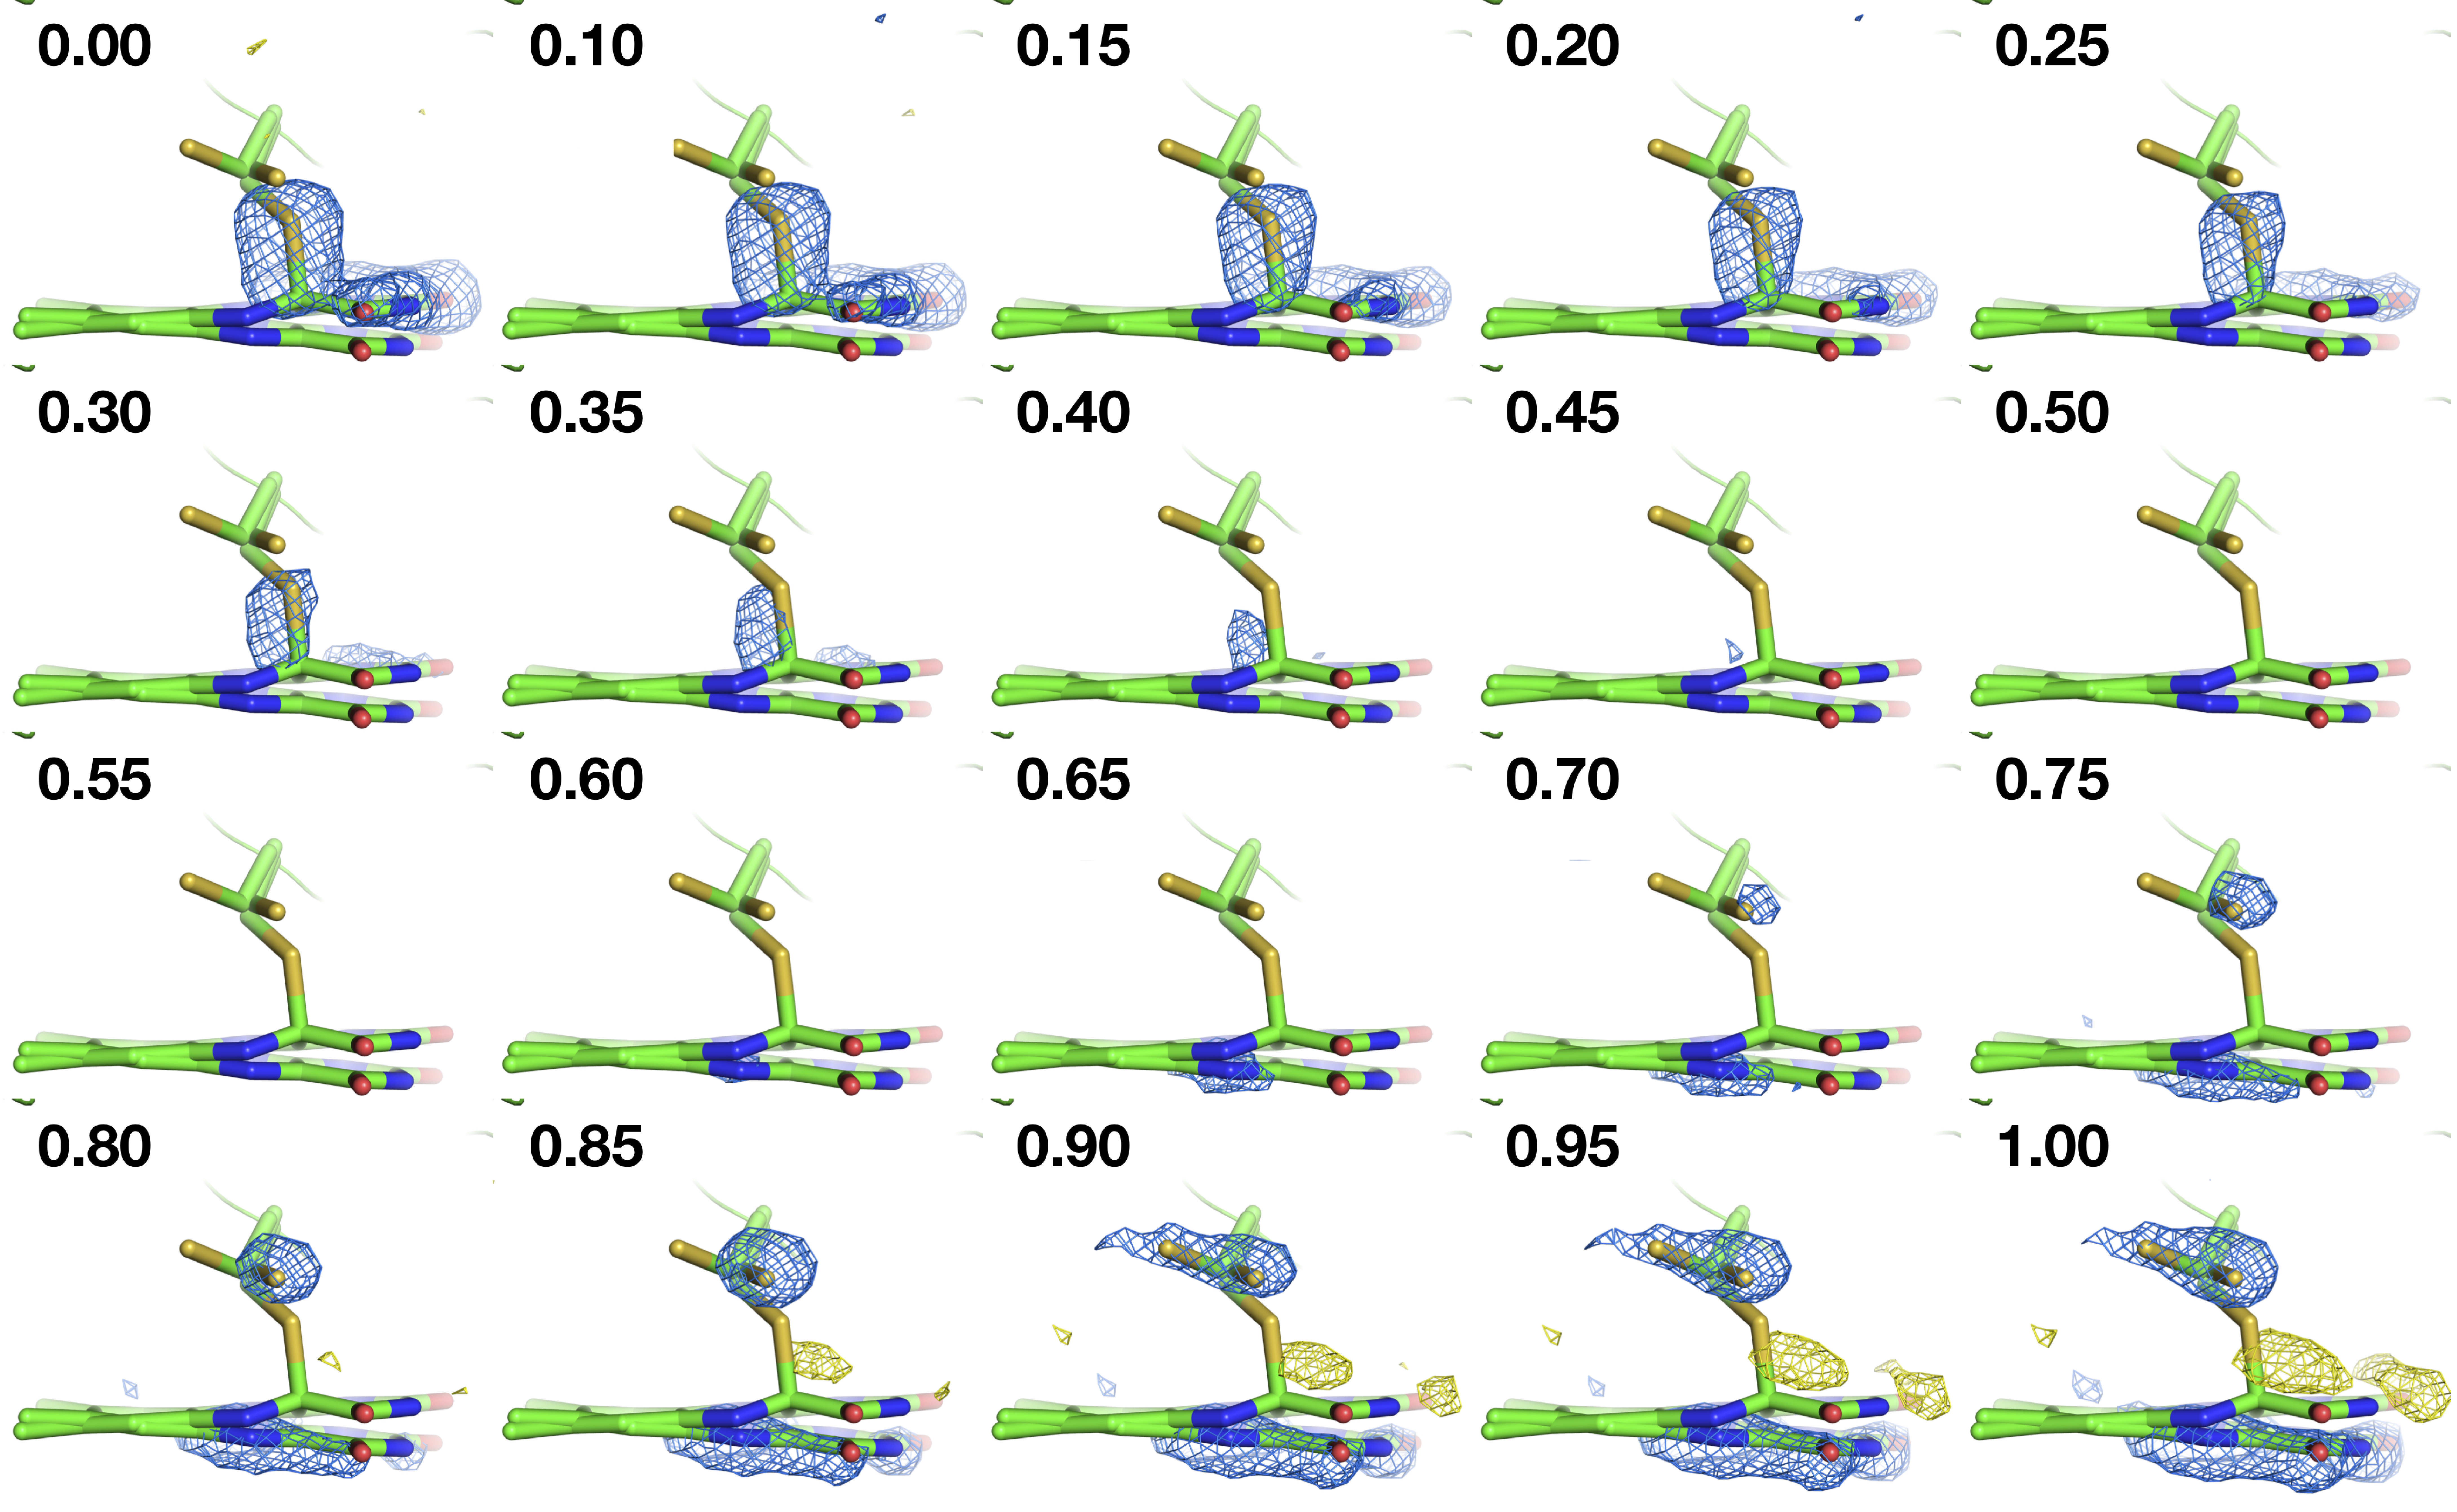
\includegraphics[width=\textwidth]{images/LOV2/FigS6.pdf}
    \hfill
    \caption{Identification of the adduct occupancy in the R\textsubscript{7”} dataset. \(F_{obs} - F_{calc}\) electron density contoured at a \(\pm 3 \sigma\) level (positive in blue and negative in yellow) around the region of the adduct for a series a chimer with adduct occupancies ranging from 0 to 1 by steps of 0.05. The occupancy minimizing difference map peaks here is 0.50.}
    \label{fig:occupancies}
\end{figure}

\section{Results}
\subsection{Experimental design}
Under blue-light irradiation, the ground state of LOV2 (called D, for dark) is first converted to a short-lived triplet state (called T, for triplet), which is then converted on a microsecond timescale to a long-lived intermediate state (called L, for light) containing a photoadduct formed by a covalent bond between the sulfur atom of a cysteine residue (C426) and the C4a carbon atom of the FMN chromophore [Fig. \ref{fig:LOV2slowexpscheme}(\textit{a})]. Constant light irradiation leads to the build up of a photostationary (PS) equilibrium between the intermediate Lstate and a state spectroscopically, but not structurally, resembling the ground state (called D'). Our study aimed to probe the relaxation of the PS equilibrium over the course of tens of minutes with a potential time resolution of \textasciitilde1 s. To this end, we applied an identical time scheme to our samples [Fig. \ref{fig:LOV2slowexpscheme}(\textit{b})], corresponding to a certain time period in the ground state (crystal or solution maintained in the dark), 1 min in the PS equilibrium (sample maintained under illumination of a blue LED brought to the sample position by the setup described in Section 2.2) and an \textasciitilde30 min period in the dark, during which the PS equilibrium relaxes to a ground state that is different from ground state D, called D''. When required, the PS equilibrium was reset at the end of the \textasciitilde30 min period with 1 min light irradiation time.

\begin{figure}[H] %bt!]
    \centering
    \noindent 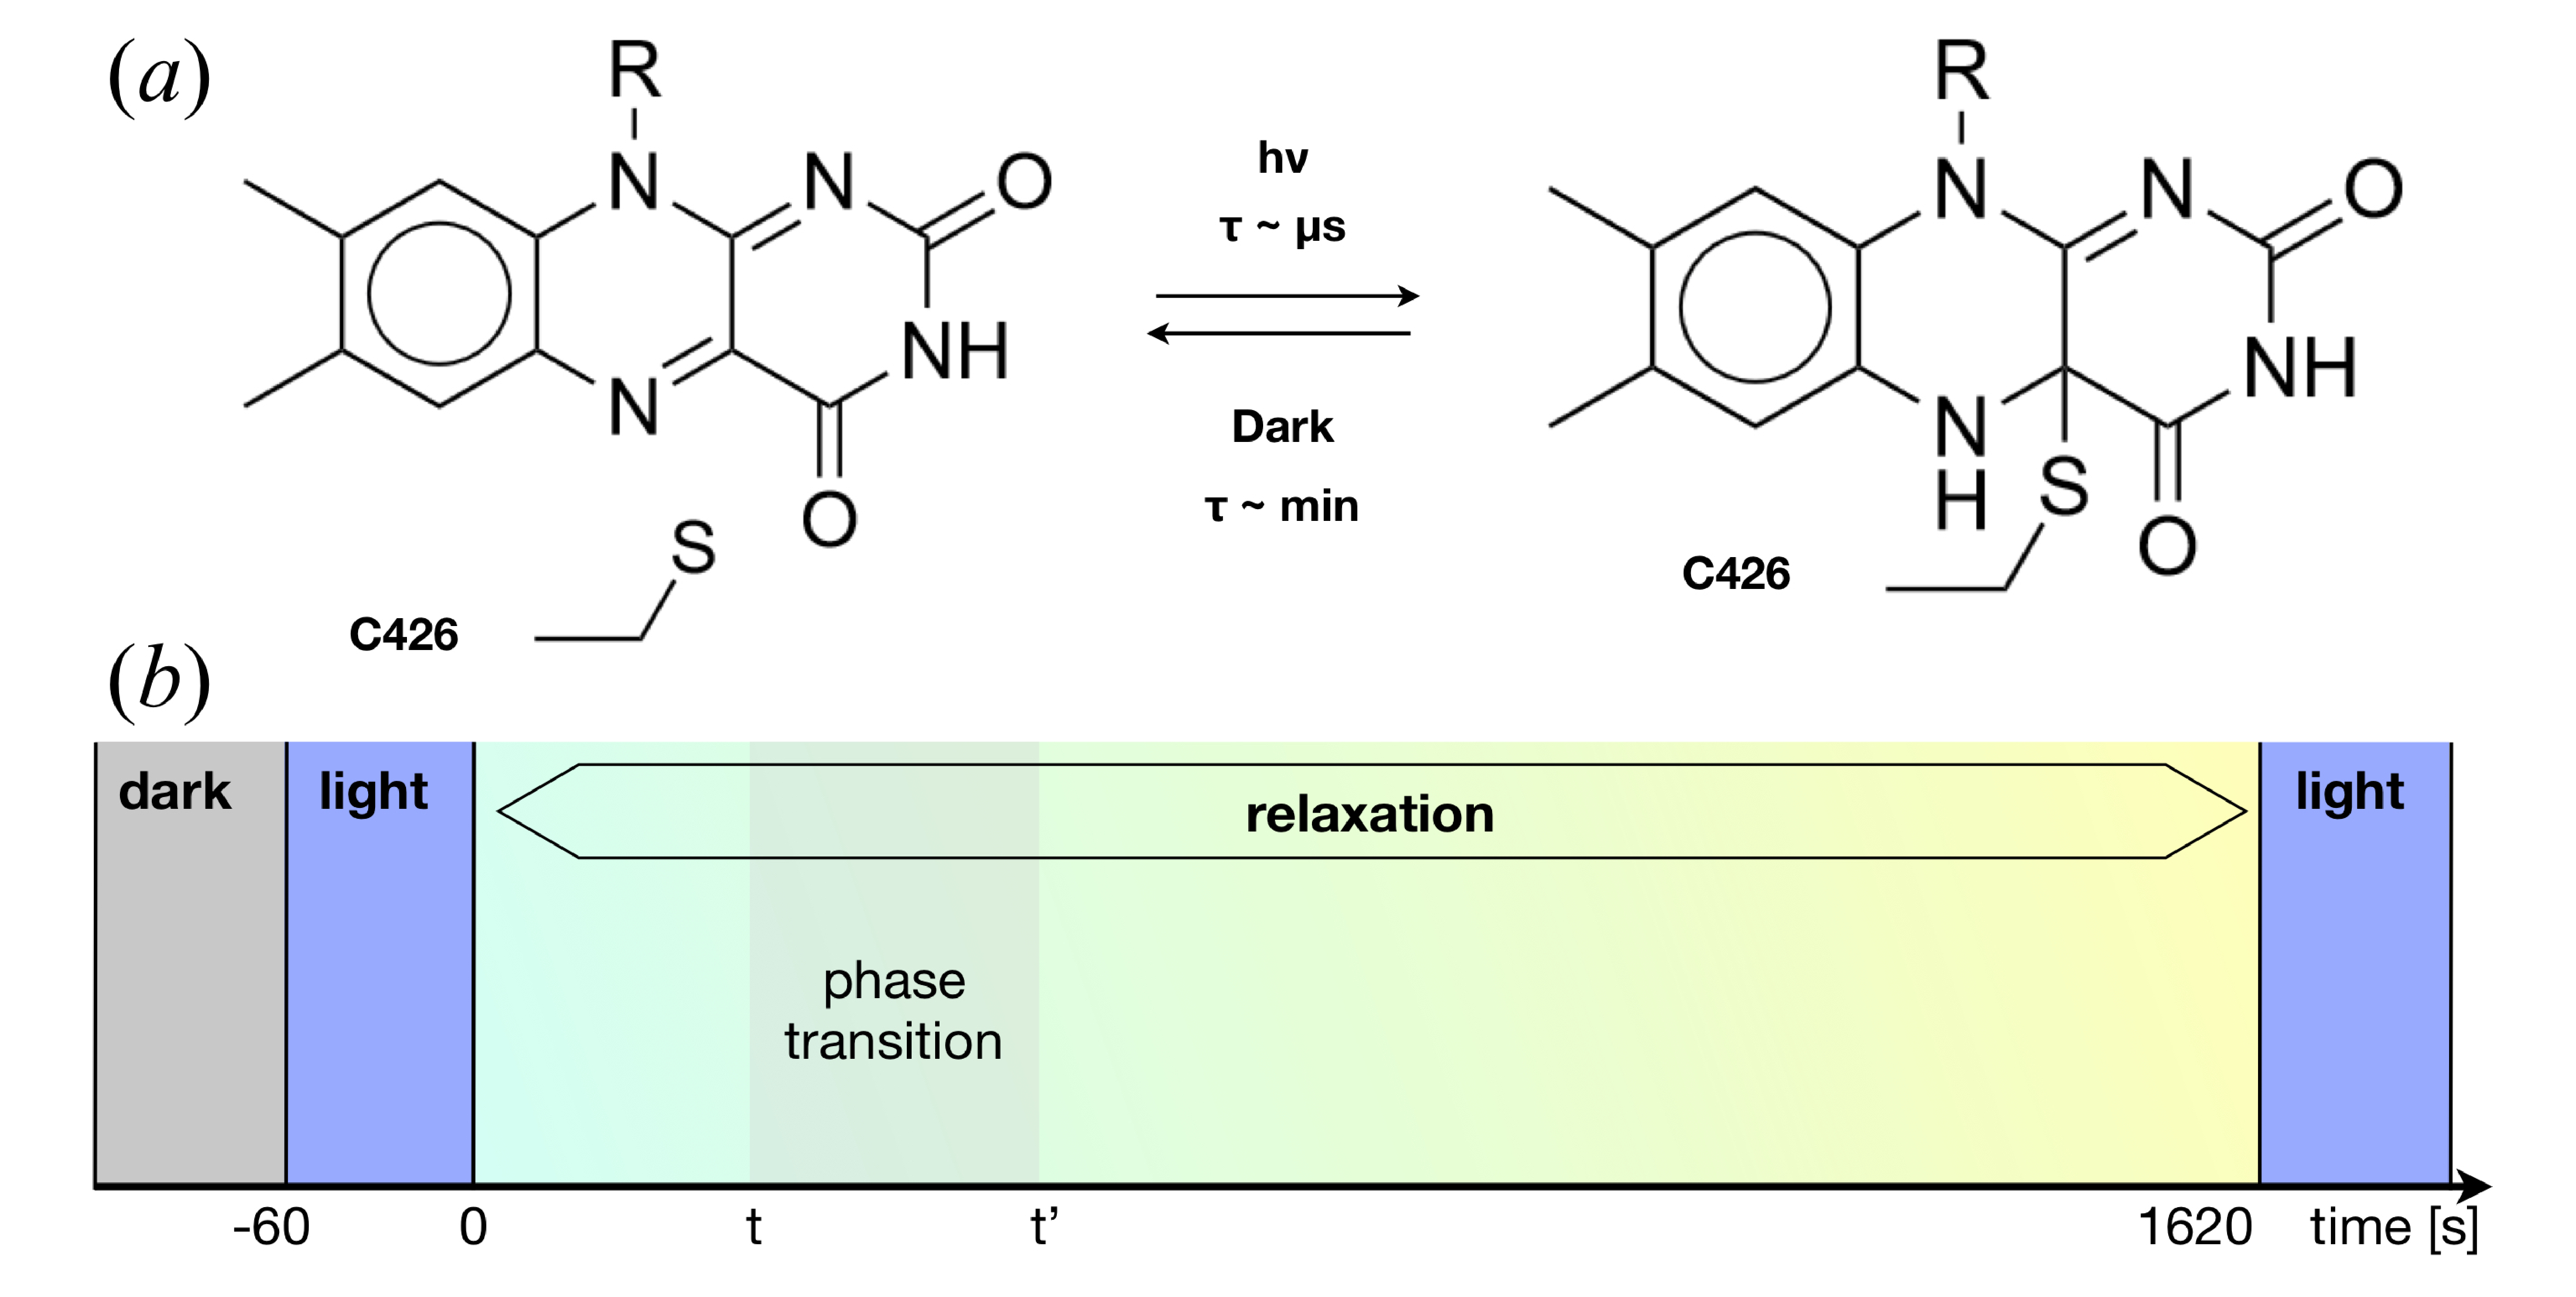
\includegraphics[width=\textwidth]{images/LOV2/LOV2slow_Fig1.pdf}
    \hfill
    \caption{\textit{a}) Reversible formation upon light irradiation of a covalent thioether bond between the sulfur atom from the C426 side chain of LOV2 and the C4a atom of the isoalloxazine ring of the FMN. (\textit{b}) Schematic of the time domains explored in this study. The ground state of LOV2 is probed in the dark (grey). A photostationary equilibrium between the ground state and the photoadduct is built up under steady blue-light illumination for 60 s (blue). Relaxation of the photoadduct is monitored over 1620 s (cyan to yellow gradient). The existence of a crystalline phase transition (light grey) is probed during the relaxation process.}
    \label{fig:LOV2slowexpscheme}
\end{figure}

A preliminary round of experiments using a similar experimental design suggested the existence of a crystalline phase transition occurring between 100 and 200 s after the end of illumination \parencite{aumonierTimeresolvedMonochromaticSynchrotron2019}. The choice of time points targeted in this study aimed to confirm this hypothesis and understand its cause, which may be related to the relaxation of the photoadduct itself. We first studied the relaxation of the PS equilibrium by UV–Vis absorption spectroscopy in concentrated solutions of LOV2, then in LOV2 crystals, to determine the relaxation time constants. We then carried out structural studies using RT-MX.
\subsection{Spectroscopic characterization of photoadduct relaxation at room temperature}
The ground state D of LOV2 absorbs maximally at 446 and 475 nm both in solution and \textit{\textit{in crystallo}} (present study), whereas the L-state absorbs maximally at 390 nm \parencite{swartzPhotocycleFlavinbindingDomain2001}. In order to monitor the relaxation of the L-state, we specifically monitored the absorbance decay at 390 nm. In solution samples, relaxation occurs with a time constant of 6.0 s [Fig. \ref{fig:LOV2slowdiffstates}(\textit{a}) and \ref{fig:LOV2slowdiffstates}(\textit{b})], whereas in crystals, it occurs around one order of magnitude slower, with a relaxation time constant of 40 s [Fig. \ref{fig:LOV2slowdiffstates}(\textit{c}) and \ref{fig:LOV2slowdiffstates}(\textit{d})], suggesting that crystal contacts slow down the formation of the ground state D''.

\begin{figure}[H] %bt!]
    \centering
    \noindent 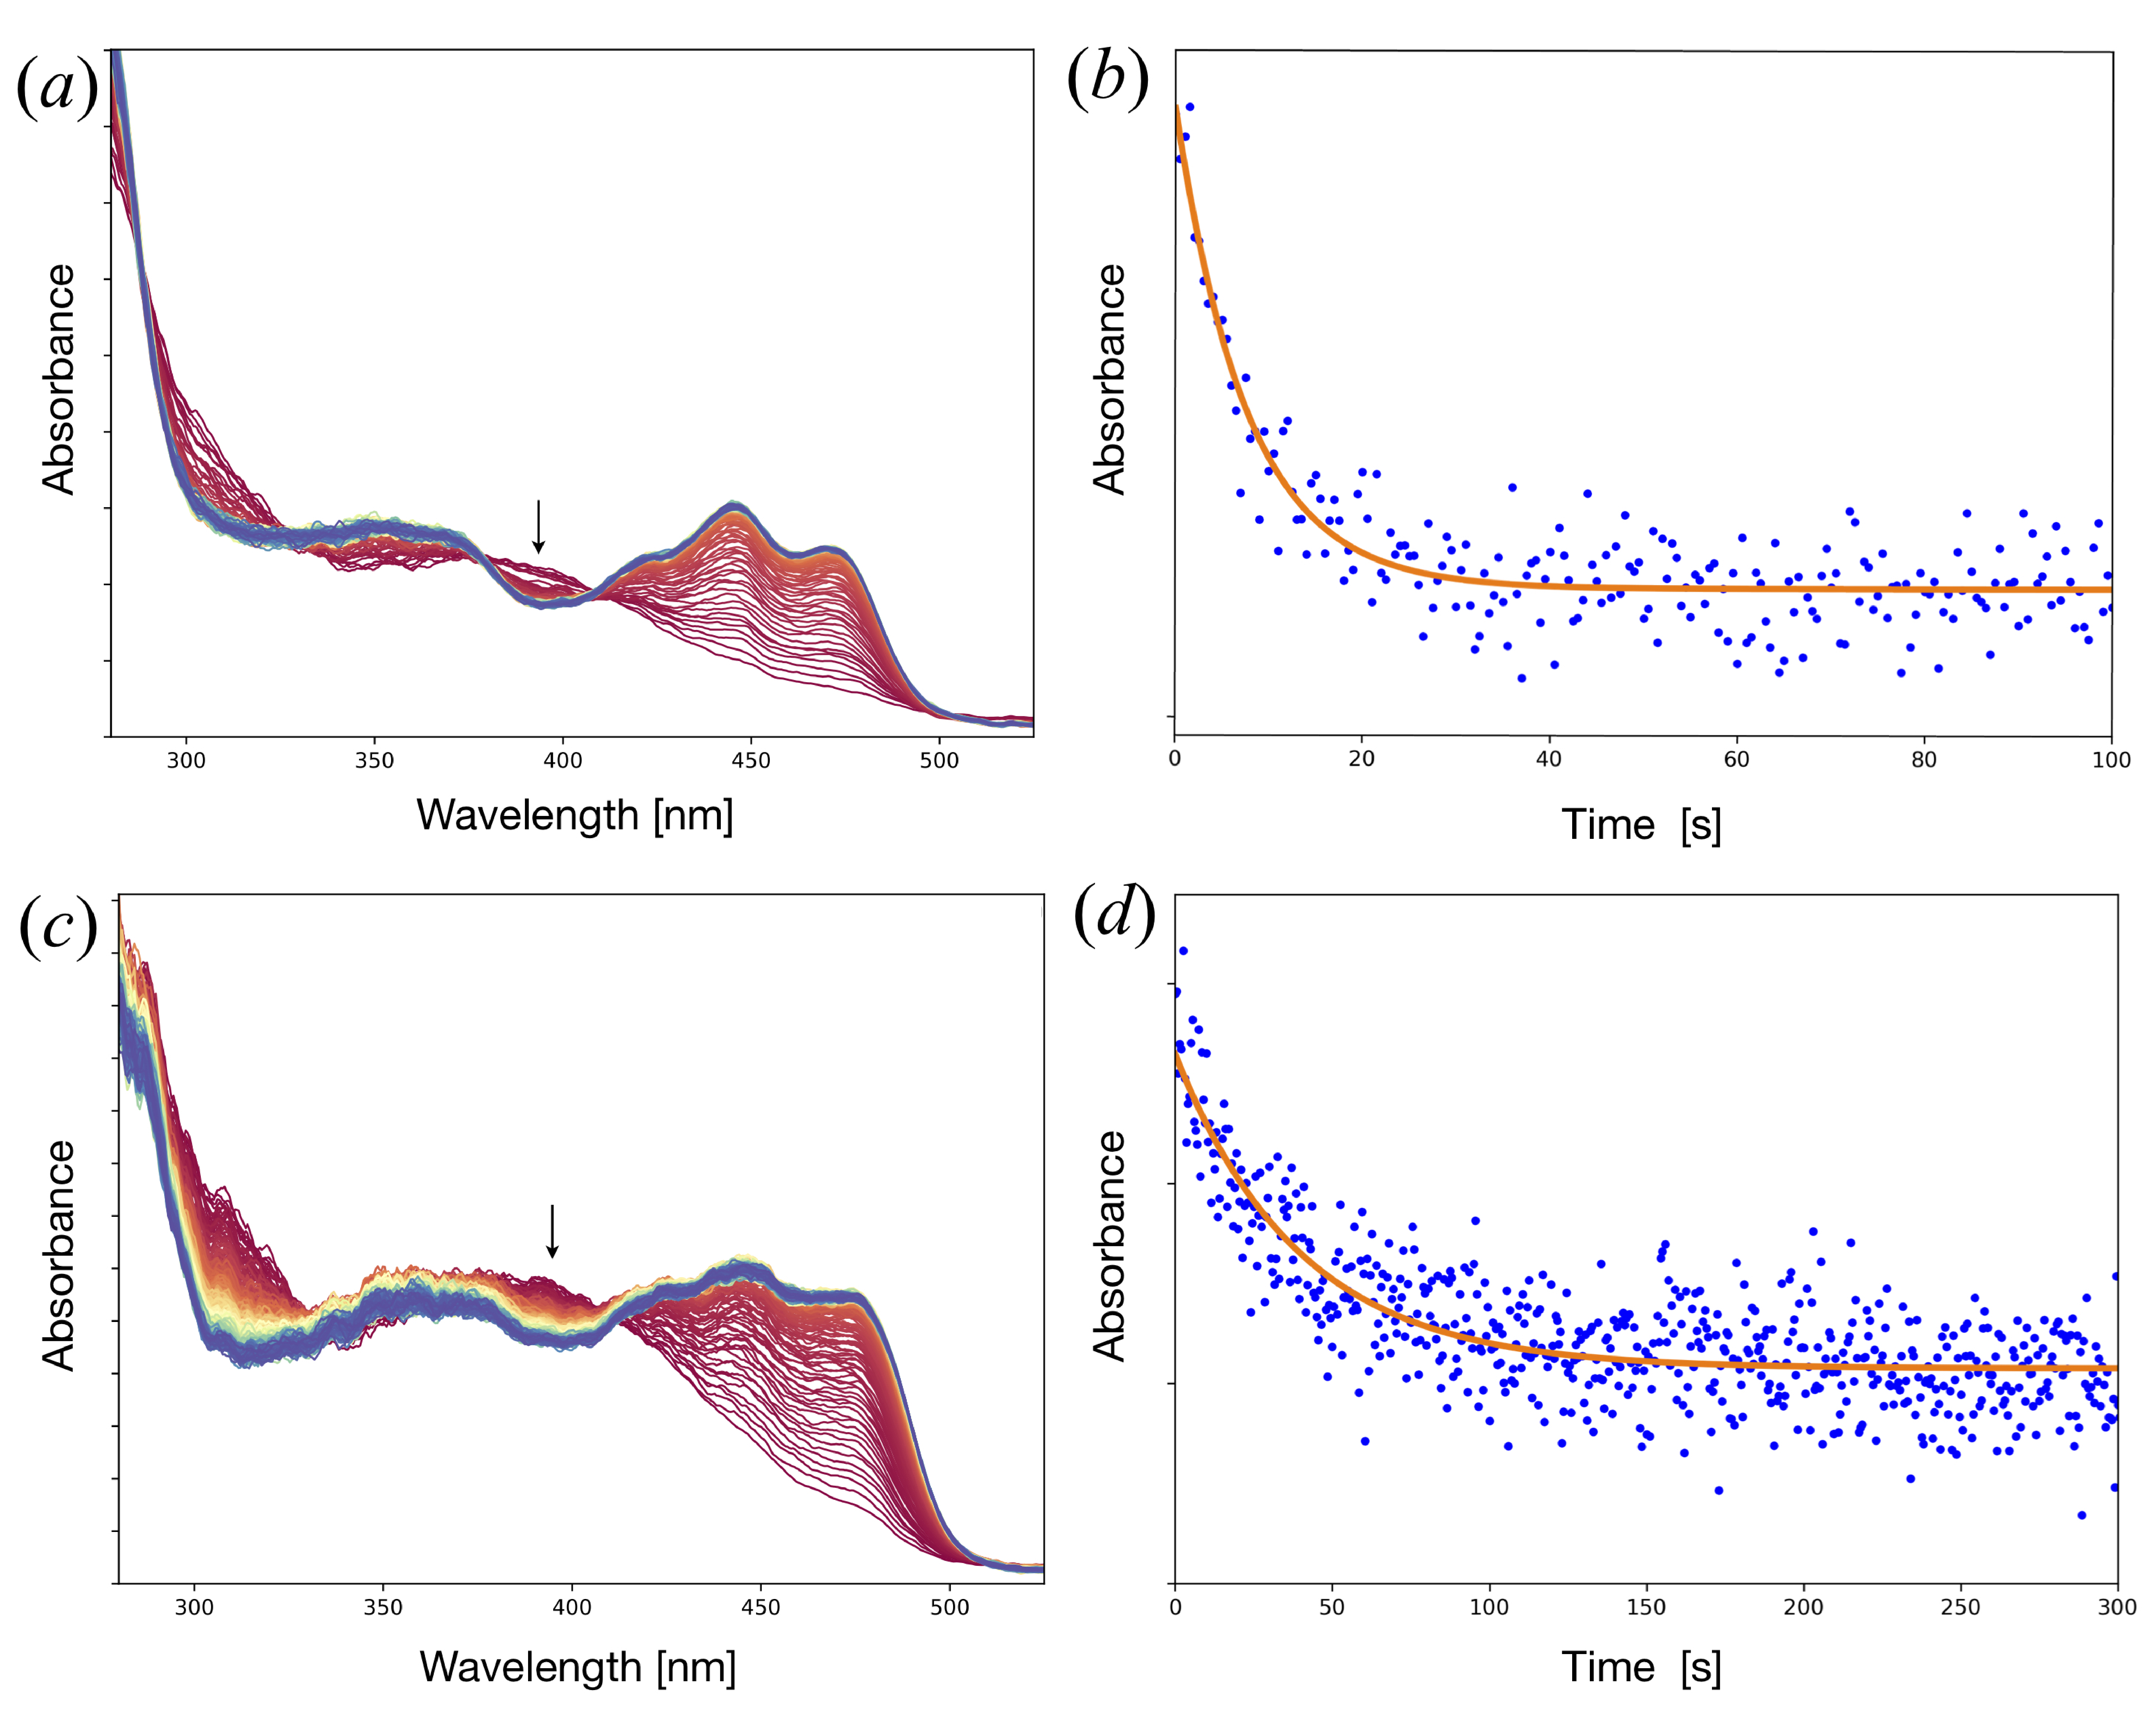
\includegraphics[width=\textwidth]{images/LOV2/LOV2slow_Fig2.pdf}
    \hfill
    \caption{PS equilibrium relaxation monitored by UV–Vis absorption spectroscopy. (\textit{a}) Time-dependent series of spectra recorded at 2 Hz from 0 s (red spectra) to 100 s (blue spectra) after the end of blue-light illumination of a solution of LOV2. (\textit{b}) Time evolution of the absorbance at 390 nm of the solution spectra shown in (\textit{a}), modelled with a monoexponential decay (red curve) with \(\tau\) = 6.0 s. (\textit{c}) Time-dependent series of spectra recorded at 2 Hz from 0 s (red spectra) to 300 s (blue spectra) after the end of blue-light illumination of a crystal of LOV2. (\textit{d}) Time evolution of the absorbance at 390 nm of the solution spectra shown in (\textit{c}), modelled with a monoexponential decay (red curve) with  =40 s}
    \label{fig:LOV2slowespectro}
\end{figure}

\subsection{Structure determination by RT crystallography of (photo)stationary states (ground and steady states)}
Before investigating the time-dependence of photoadduct relaxation and the existence of the crystalline phase transition, we determined the reference structures with the highest resolution possible for (i) the ‘true’ ground state D from unilluminated crystals, (ii) the structural description of the PS equilibrium consisting of a ratio of the L-state and a pseudo ground state D', and (iii) the ground state D'' recovered over a time period (1620 s) much longer than both the decay time constant determined by spectroscopy (40 s) and the appearance of the expected crystalline phase transition (<200 s).
\subsubsection{Structural differences between the ground-state component D' of the PS equilibrium and the D-state.}
A characteristic of the structure of the ground state D, determined at 1.58 \AA\ resolution at room temperature in the space group \textit{P}4\textsubscript{3}2\textsubscript{1}2 to \textit{P}2\textsubscript{1}2\textsubscript{1}2\textsubscript{1} (Table S1), is the presence of two alternate conformations A (major) and B (minor) of the C426 side chain [Fig. \ref{fig:LOV2slowdiffstates}(\textit{a})] and a well ordered C-terminus folded into a short \textalpha-helix (Fig. S2). We then recorded datasets under conditions yielding the PS equilibrium, i.e. under constant illumination initiated at least 1 min before data collection. The seven resulting datasets were determined in the space group \textit{P}4\textsubscript{3}2\textsubscript{1}2 to \textit{P}2\textsubscript{1}2\textsubscript{1}2\textsubscript{1} at a resolution between 1.73 and 2.23 \AA. We deposited the best compromise in terms of resolution, data reduction quality and L-state occupancy, which varied between 60 and 90\%. The combination of two states (D' and L) in the crystals made model building somewhat difficult. To facilitate manual rebuilding, and because the D and PS datasets were not isomorphous, we calculated Fourier difference maps between PS datasets and datasets recorded at early time points of the time-resolved series (see thereafter), highlighting very clearly the reorganization of side chains, whole residues and stretches of residues (Fig. \ref{fig:LOV2slowQ489mech}). We thus obtained a representative structure of the PS equilibrium, which consists of 60 to 90\% L-state structure (see Section 3.3.2) and 10 to 40\% pseudo ground D'state structure, which differs from the D-state structure by the conformation of C426 (one single conformation A versus conformations A and B) [Fig. \ref{fig:LOV2slowdiffstates}(\textit{b})] and a fully disordered C-terminus starting from residue 496 [Fig. \ref{fig:LOV2slowdiffstates}(\textit{e})]. In addition, the precise orientation of the Q489 side chain in D', which is hydrogen-bonded to a carbonyl group of the FMN in D [Fig. \ref{fig:LOV2slowdiffstates}(\textit{a})], cannot be ascertained from our data [question mark in Fig. \ref{fig:LOV2slowdiffstates}(\textit{b})].

\begin{figure}[H] %bt!]
    \centering
    \noindent 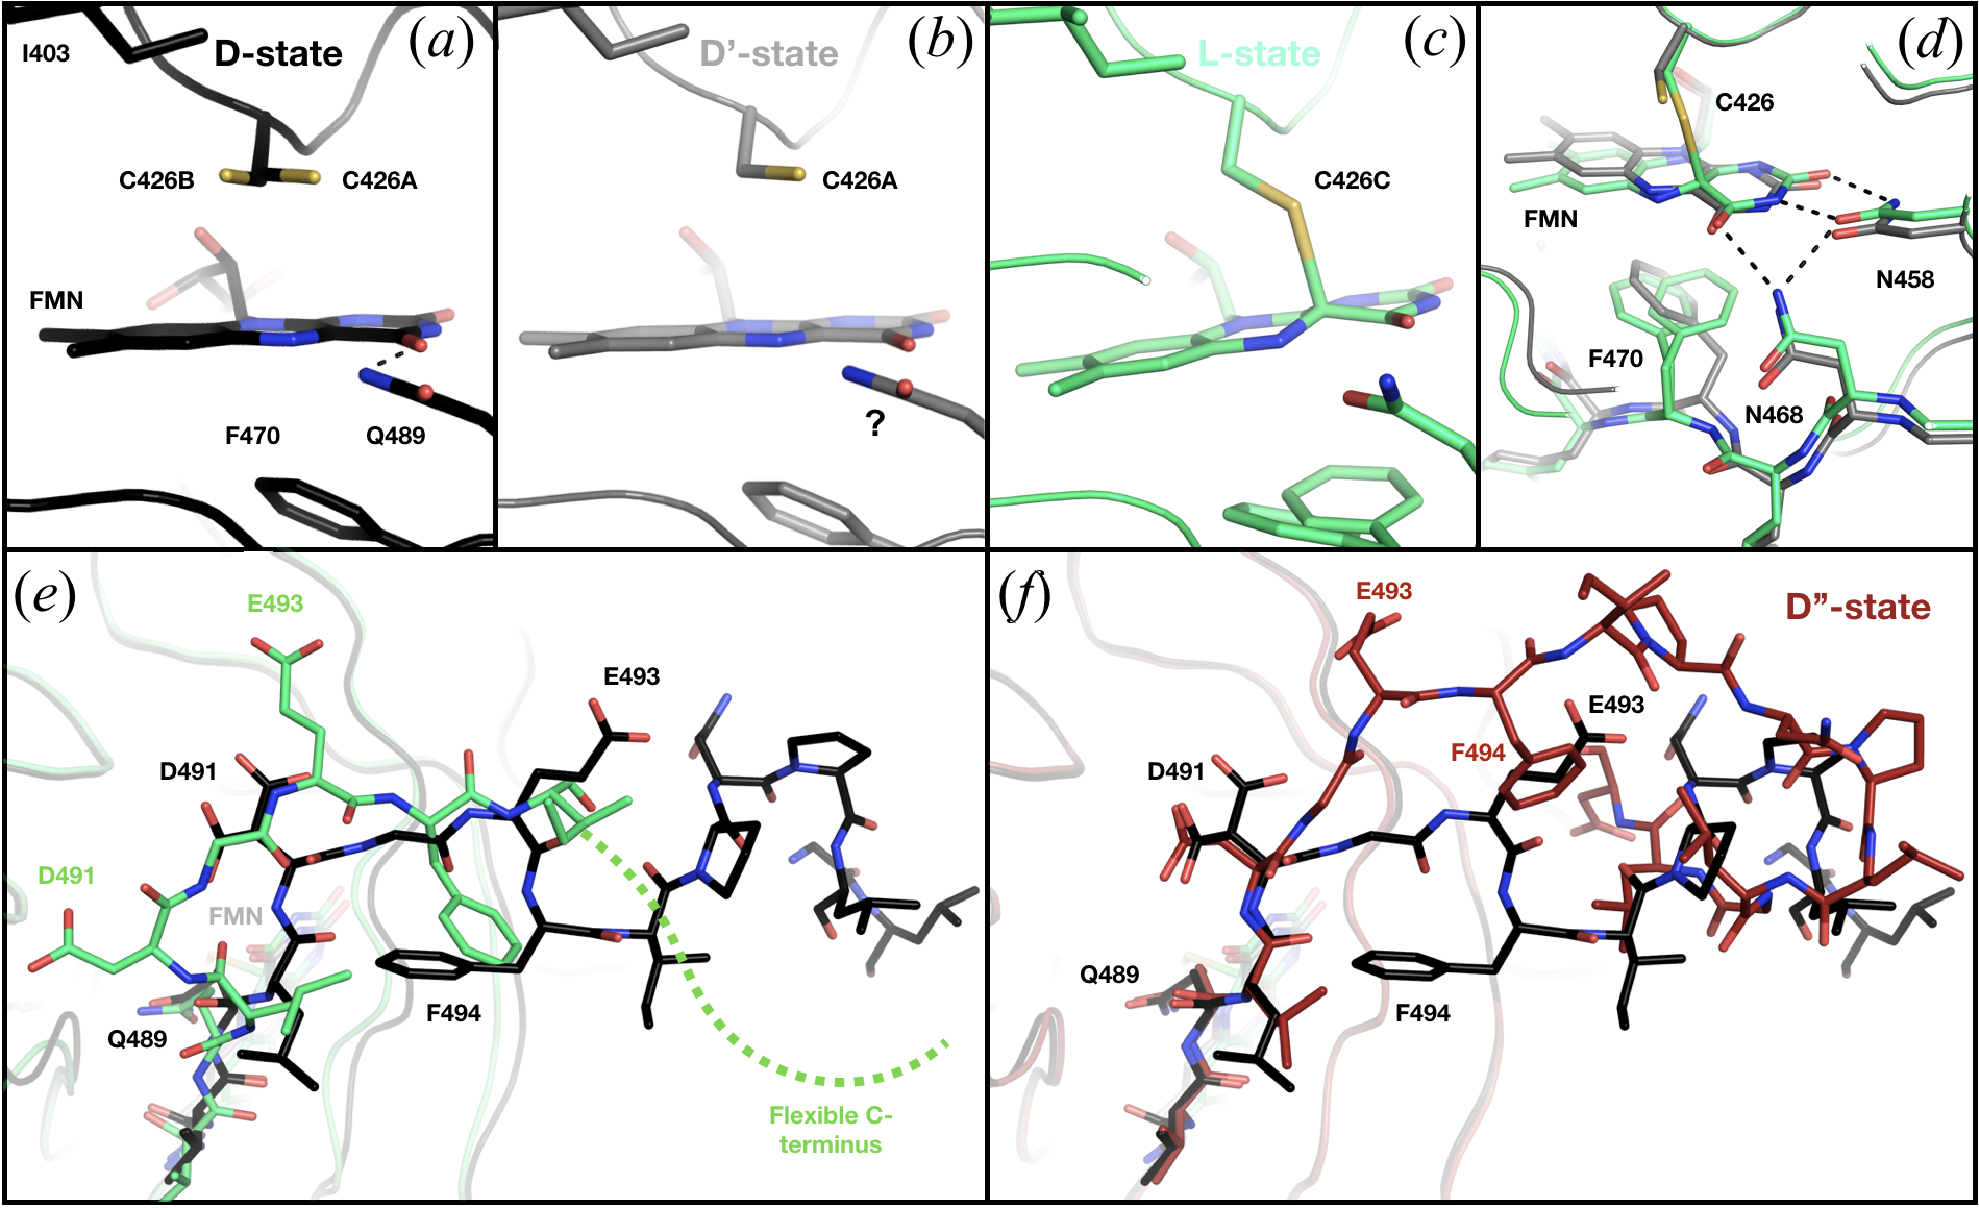
\includegraphics[width=\textwidth]{images/LOV2/LOV2slow_Fig3.pdf}
    \hfill
    \caption{Comparison of the various structures of the ground state and that of the L-state intermediate. Chromophore environments in (\textit{a}) the ‘true’ ground state structure D (carbon atoms in black), (\textit{b}) the ground state structure D' present in the PS equilibrium (carbon atoms in grey) and (\textit{c}) the intermediate state structure L present in the PS equilibrium (carbon atoms in green). The question mark in panel (\textit{b}) illustrates the fact that the precise orientation of the Q489 side chain in D' cannot be ascertained from our data. C426 has two conformations in D, and only one in D'.(\textit{d}) Superposition of the D' and L structures on one side of the chromophore in the PS equilibrium. (\textit{e}) Comparison of the conformation of the C-terminus in D and L. In D, residues 496 to 502 form a short \textalpha-helix, which cannot be modelled in either of the structures of the PS equilibrium. (\textit{f}) Comparison of the structure of the C-terminus in D(\textalpha-helical) and in one of the two molecules of D'' (hook-shaped, firebrick).}
    \label{fig:LOV2slowdiffstates}
\end{figure}

\subsubsection{Structural differences between the L-state and the D-state.}
In the L-state structure, C426 is engaged in a covalent bond with atom C4a of the FMN [Fig. \ref{fig:LOV2slowdiffstates}(\textit{c})]. Our data do not allow us to unambiguously determine the \textasciitilde180\degree  rotation of the Q489 head group observed for other LOV domains, but at the minimum, the distance between the N"2 atom of Q489 and the O4 atom of the FMN has increased, supporting the documented loss of the hydrogen bond \parencite{iulianoUnravelingMechanismLOV2020}. This is coupled with an upward movement of the hydrophilic side of the isoalloxazine ring of the FMN, triggering side-chain rearrangements [Fig. \ref{fig:LOV2slowdiffstates}(\textit{d})] which propagate to the C-terminus, eventually leading to disordering [Fig. \ref{fig:LOV2slowdiffstates}(\textit{e})]. The disordering of the C-terminus is concomitant with a marked reorganization of the N-terminus spearheaded by the reorientation of D491, located at the beginning of the C-terminus (Fig. S3).

\begin{figure}[H] %bt!]
    \centering
    \noindent 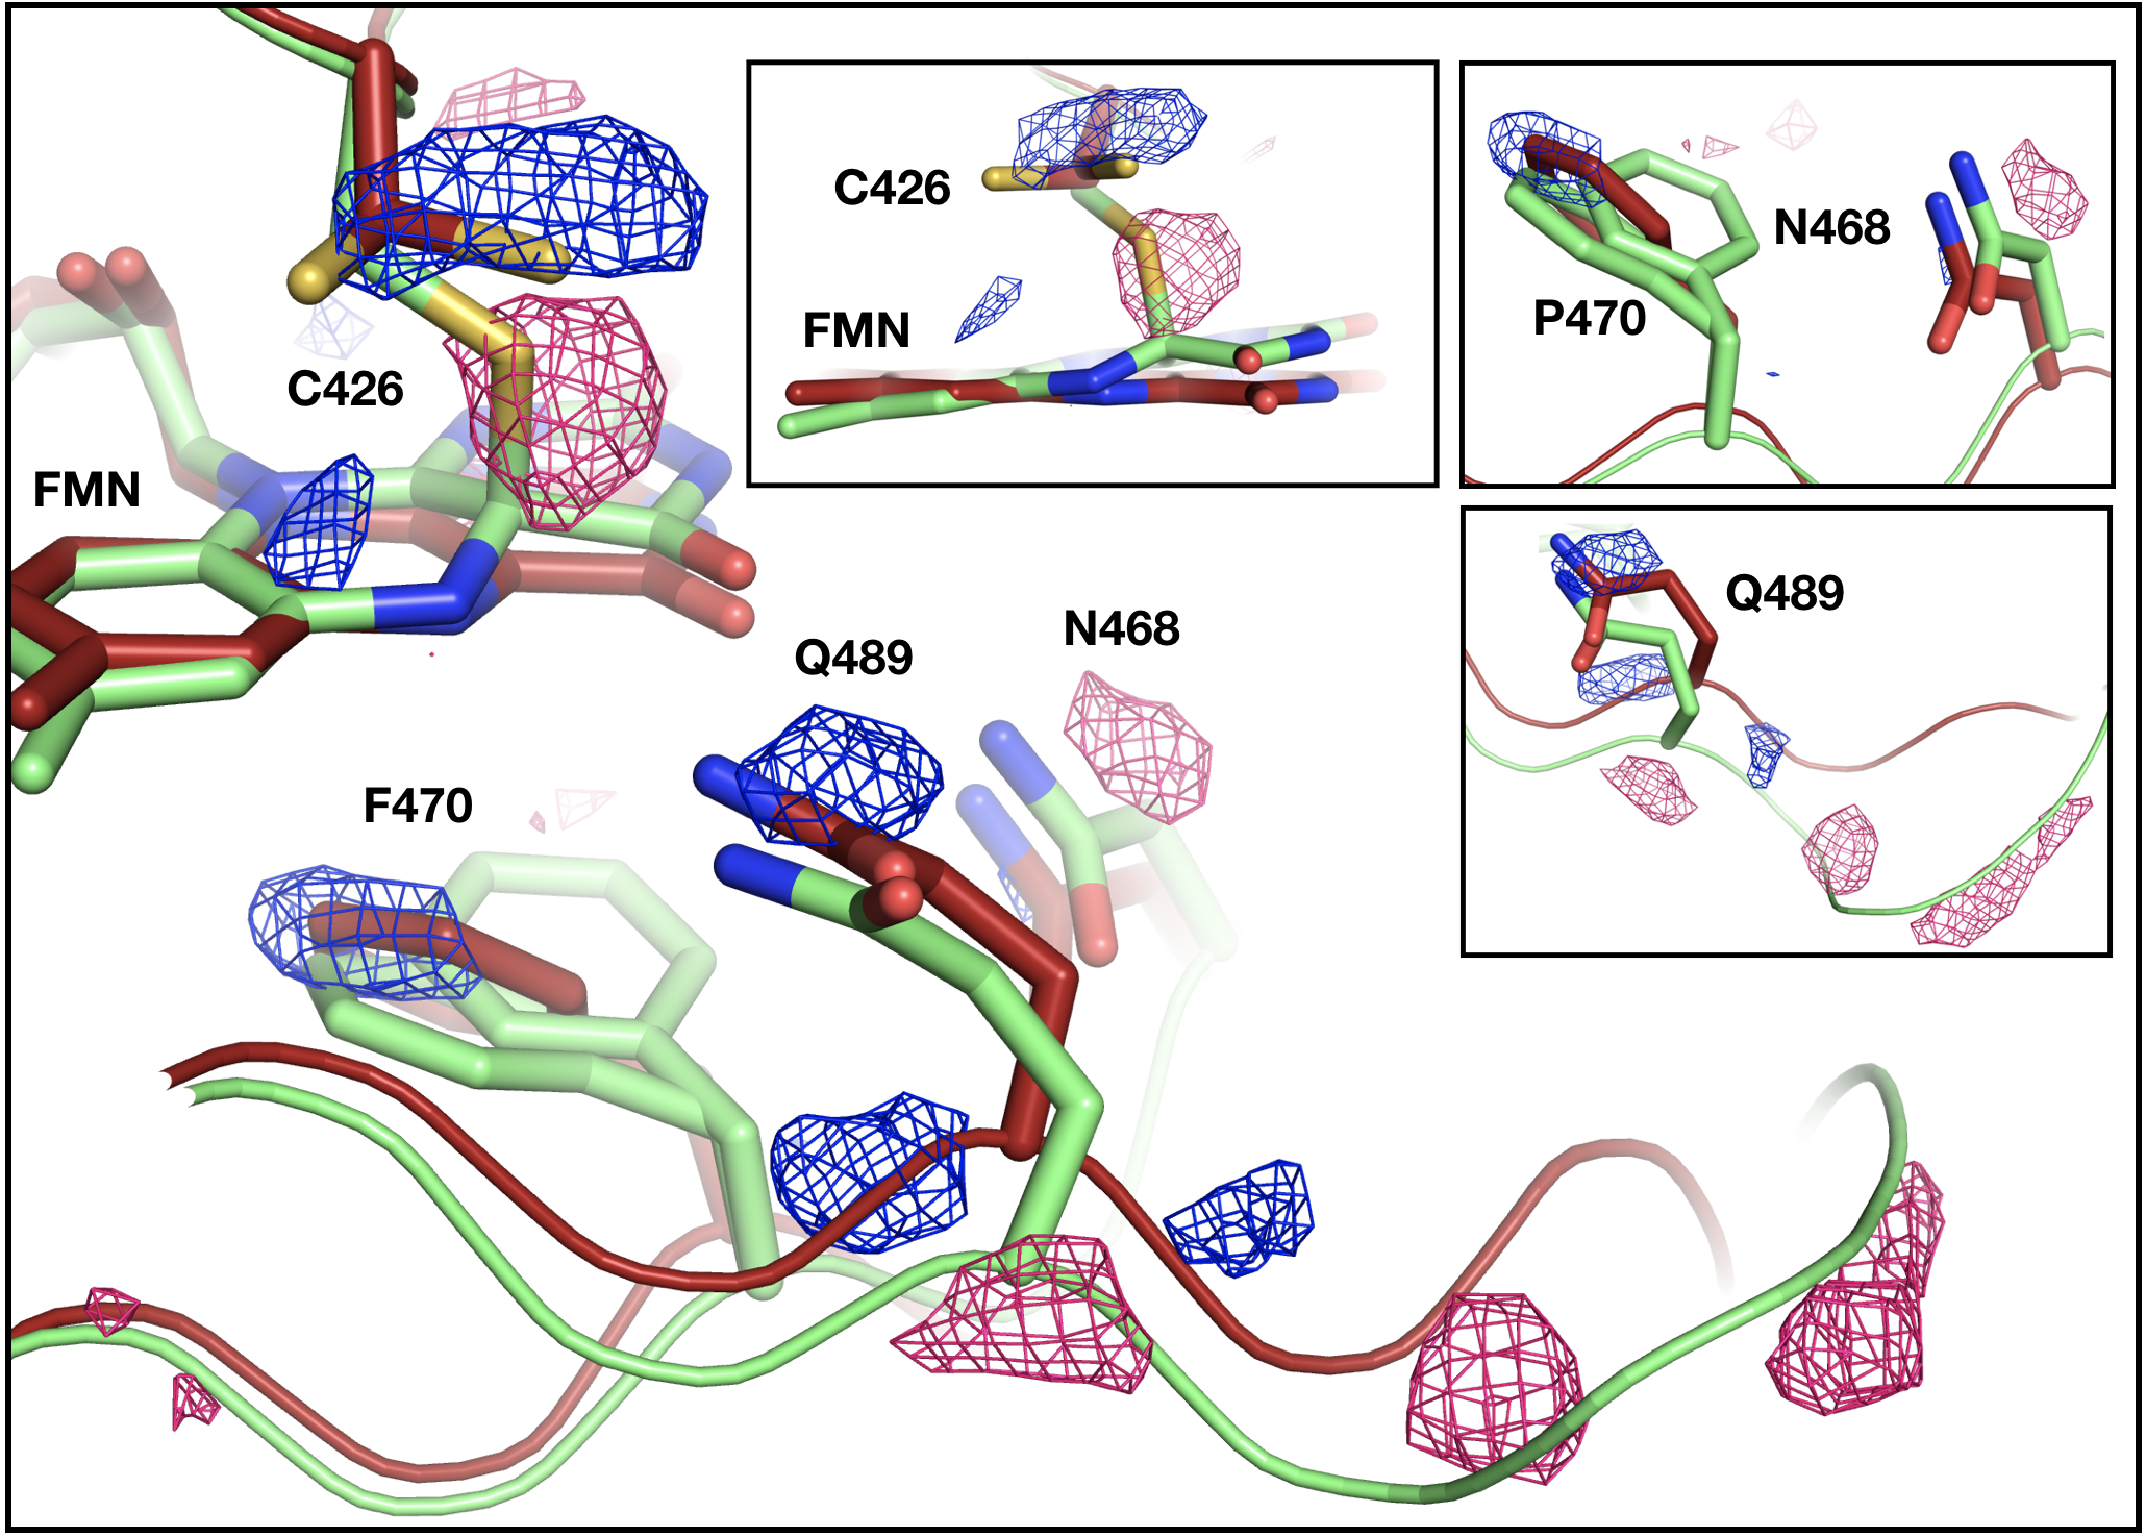
\includegraphics[width=\textwidth]{images/LOV2/LOV2slow_Fig4.pdf}
    \hfill
    \caption{Identification of structural rearrangements around the FMN occurring during the relaxation process. Fourier difference map calculated between R\textsubscript{35''} and a dataset for the PS equilibrium. Positive and negative peaks are displayed as blue and dark pink meshes, respectively. The L-state (green) and D''-state (firebrick) models are displayed as ribbons and sticks. Alternate orientations for key residues are shown as insets.}
    \label{fig:LOV2slowQ489mech}
\end{figure}

\subsubsection{Crystal phase transition leading to a different ground state structure D''}
While all datasets corresponding to the ground state D and to the PS equilibrium could be indexed and reduced in the space group \textit{P}4\textsubscript{3}2\textsubscript{1}2 to \textit{P}2\textsubscript{1}2\textsubscript{1}2\textsubscript{1} with one monomer in the asymmetric unit, the dataset corresponding to the end of the relaxation period we probed (see Fig. S3), and thus to a return to the ground state, can only be indexed and reduced in the space group \textit{P}2\textsubscript{1}2\textsubscript{1}2\textsubscript{1} with a dimer in the asymmetric unit. 

\begin{figure}[H] %bt!]
    \centering
    \noindent 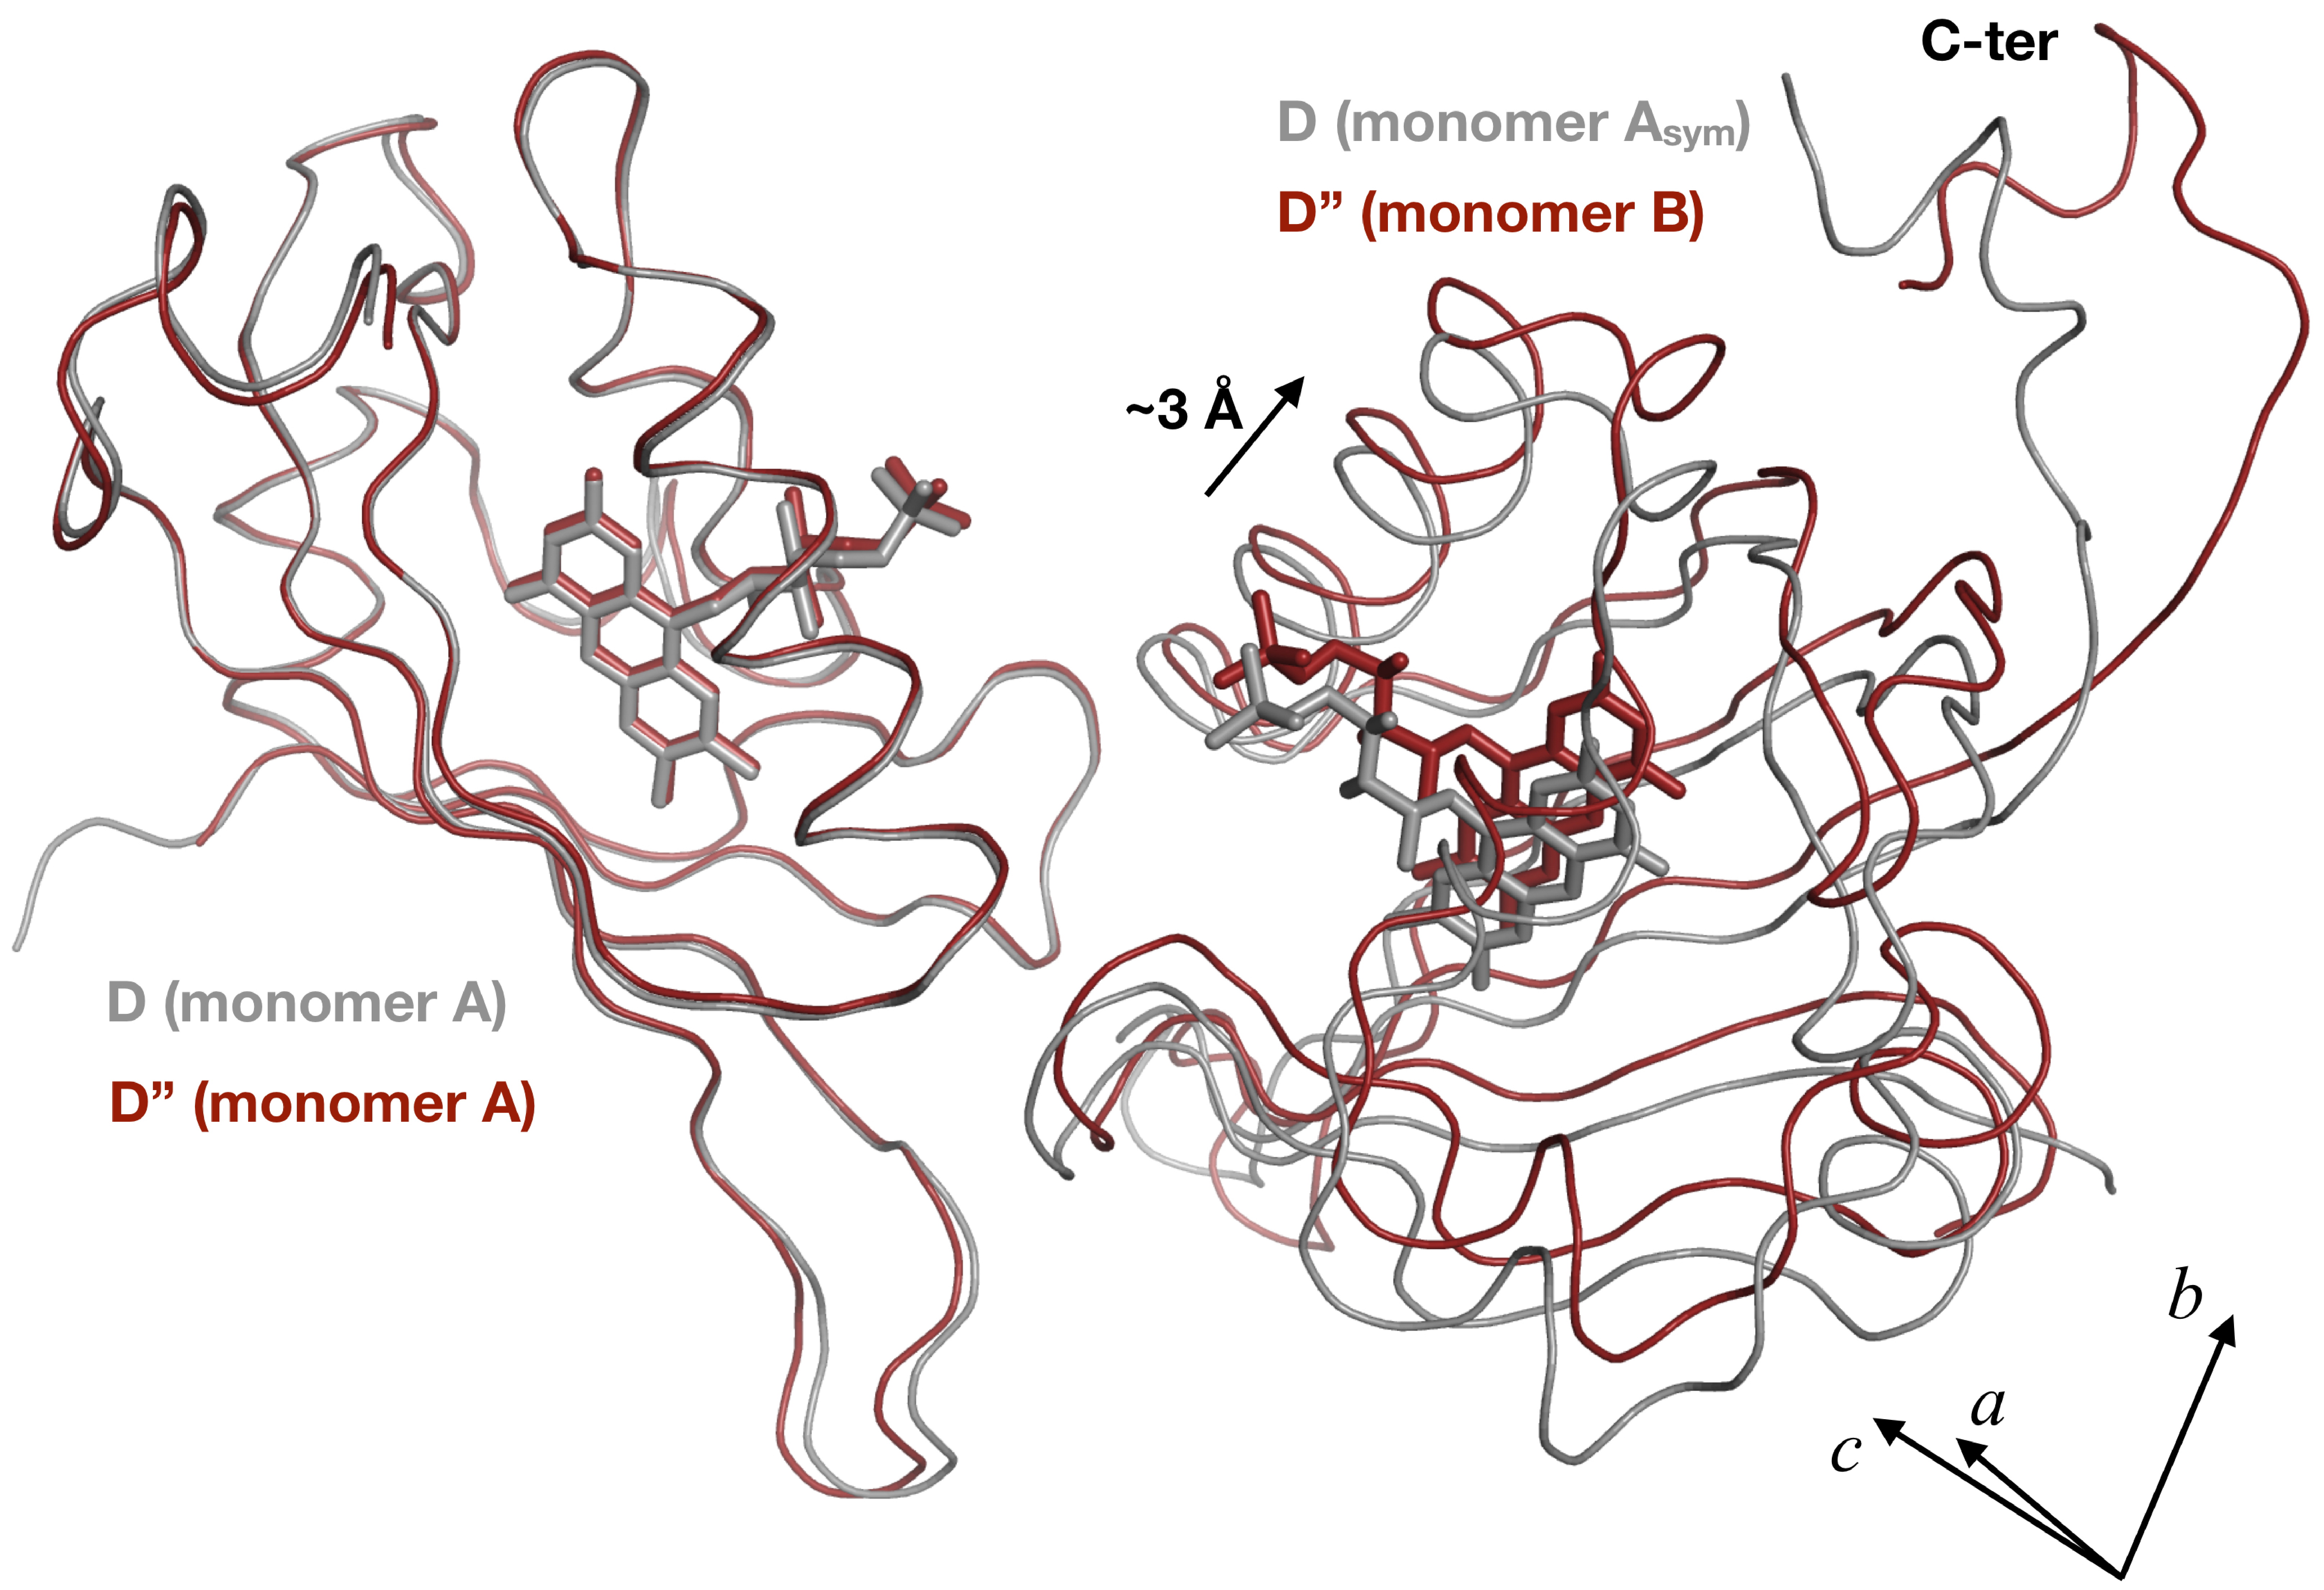
\includegraphics[width=\textwidth]{images/LOV2/LOV2slow_Fig5.pdf}
    \hfill
    \caption{Comparison of the crystallographic dimer from the dark structure D (grey ribbon) with the non-crystallographic dimer from structure D'' (firebrick ribbon). Both dimers were superposed on their chain A. A translation of \textasciitilde3\AA\  between chain Asym (from D) and chain B (from D'') along the b axis is reported.}
    \label{fig:LOV2slowtwodark}
\end{figure}

In practice, this corresponds to the loss of one symmetry element in the crystal. Both monomers A and B of the dimer show complete absence of the photoadduct, demonstrating that the time point corresponds a new ground state D'' that is structurally different from D. They differ significantly in the conformation of their C-termini, which, in monomer A, exhibits the \textalpha-helical conformation observed in the D structure but, in monomer B, adopts a hook-shaped structure [Figs. 3( f) and S4]. When comparing the crystal packing in both ground state structures, the non-crystallographic dimer of D'' differs from the crystallographic dimer observed in D by an \textasciitilde3\AA\ translation of chain B, which amounts to a subtle sliding of one molecule compared with the other [Fig. \ref{fig:LOV2slowtwodark}]. This leads to the crystal lattice offering different volumes to the two C-termini of the crystallographic dimer, the larger corresponding to the less structured, hook-shaped C-terminus.

\begin{figure}[H] %bt!]
    \centering
    \noindent 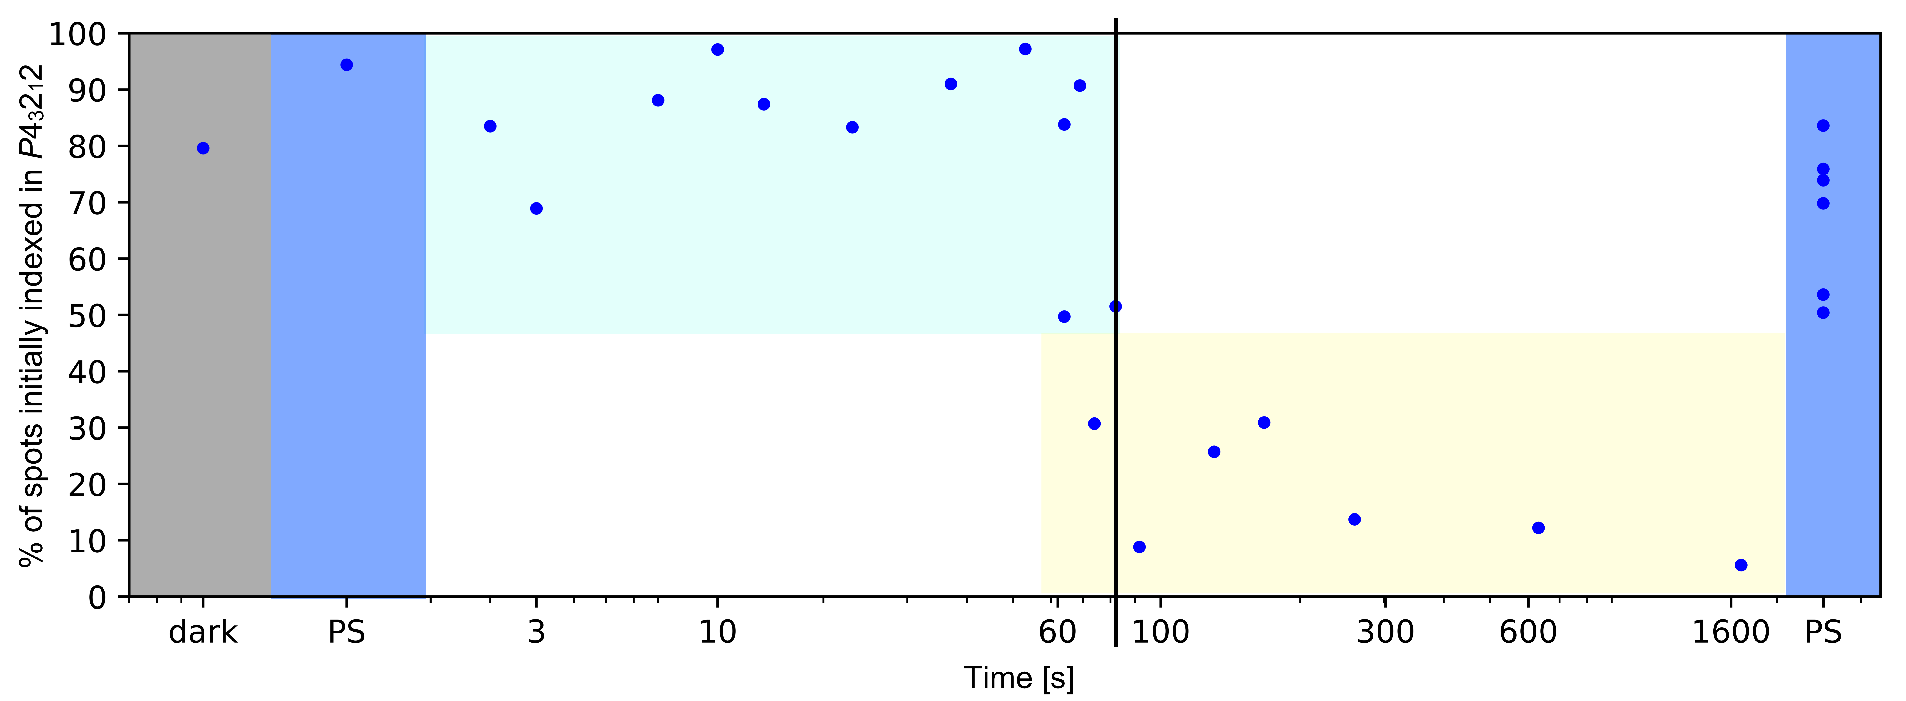
\includegraphics[width=\textwidth]{images/LOV2/LOV2slow_Fig6.pdf}
    \hfill
    \caption{Initial indexing of the various datasets recorded along the illumination scheme. Each dataset was indexed by autoPROC with the space group \textit{P}4\textsubscript{3}2\textsubscript{1}2 to \textit{P}2\textsubscript{1}2\textsubscript{1}2\textsubscript{1} as input. The percentage of spots indexed in the space group \textit{P}4\textsubscript{3}2\textsubscript{1}2 to \textit{P}2\textsubscript{1}2\textsubscript{1}2\textsubscript{1} is represented as a function of time on a logarithmic timescale. All datasets recorded prior to, and during illumination can be confidently indexed in the space group \textit{P}4\textsubscript{3}2\textsubscript{1}2 to \textit{P}2\textsubscript{1}2\textsubscript{1}2\textsubscript{1} (>50\%). Datasets recorded during the first 60 to 80 s of the relaxation step also show a majority of spots initially indexed in the space group \textit{P}4\textsubscript{3}2\textsubscript{1}2 to \textit{P}2\textsubscript{1}2\textsubscript{1}2\textsubscript{1}. However, after 60 s, datasets begin to have less than 50\% spots initially indexed in the tetragonal space group. For late time points (above 200 s), datasets exhibit an indexing percentage in the space group \textit{P}4\textsubscript{3}2\textsubscript{1}2 to \textit{P}2\textsubscript{1}2\textsubscript{1}2\textsubscript{1} below 15\% and can only be reliably indexed and reduced in the space group \textit{P}2\textsubscript{1}2\textsubscript{1}2\textsubscript{1}. The fact that all datasets recorded during a second illumination step can be indexed in the space group \textit{P}4\textsubscript{3}2\textsubscript{1}2 to \textit{P}2\textsubscript{1}2\textsubscript{1}2\textsubscript{1} demonstrates the reversibility of the space group conversion.}
    \label{fig:LOV2slowindexP4}
\end{figure}

\subsection{Probing LOV2 dynamics by time-resolved oscillation crystallography}
We investigated the time-dependence of photoadduct relaxation and the existence of the crystalline phase transition by recording 1.2 s datasets at various delays after switching off actinic illumination, thus releasing the PS equilibrium. We recorded 18 datasets corresponding to delays of 2, 3, 7, 10, 13, 21, 35, 51, 62 (x2), 67, 72, 80, 90, 130, 166, 258, 630 and 1620 s at resolutions between 1.65 and 2.47 \AA. Datasets were named R\textsubscript{2''}, R\textsubscript{3''}, ... and R\textsubscript{1620''}. Note thatR\textsubscript{1620''} corresponds to the D''-state mentioned in Section 3.3. Data were best reduced in the space group \textit{P}4\textsubscript{3}2\textsubscript{1}2 to \textit{P}2\textsubscript{1}2\textsubscript{1}2\textsubscript{1} for all datasets recorded before 67 s and for the dataset recorded at t = 80 s (Fig. \ref{fig:LOV2slowindexP4}). Data were best reduced in the space group \textit{P}2\textsubscript{1}2\textsubscript{1}2\textsubscript{1} for the dataset recorded at t = 72 s and for all datasets recorded after 90 s (Fig. \ref{fig:LOV2slowindexP4}). This indicates that the expected crystal phase transition occurs in the 67–80 s time window, significantly earlier and narrower than identified in our preliminary experiments. For comparative analysis purposes, all datasets were eventually reduced in the space group \textit{P}2\textsubscript{1}2\textsubscript{1}2\textsubscript{1}, so as to be able to detect any small differences occurring to either molecules of the dimer in the asymmetric unit at earlier time points.
\subsubsection{Photoadduct relaxation}
The variation of unit-cell parameters with time (Table S1) illustrates that datasets at individual time points are not sufficiently isomorphous with others in the series to allow for the calculation of both Fourier difference maps with a high signal-to-noise ratio and reliable extrapolated structure factors. We thus devised a refinementbased method to confidently derive the proportion of the various intermediate states (L-state and D''-state) at each time point. A series of models were generated with two alternate conformations (one corresponding to the L-state, one to the D0-state) for key residues (I403, I421, C426, L429, I446, F470, Q489) and the FMN chromophore, with respective occupancies varying from 0/100\% to 100/0\% in steps of 5\%. For each of the R\textsubscript{xxxx''} datasets reduced in the space group \textit{P}2\textsubscript{1}2\textsubscript{1}2\textsubscript{1}, each of these 21 models was subject to molecular replacement, followed by rigid body and individual \textit{B}-factor refinement. \textit{F}\textsubscript{obs} - \textit{F}\textsubscript{calc} electron density maps were visually inspected at sigma levels down to 2.0 \AA\ to identify the likeliest combination of occupancies (Fig. S5). In a second step, we investigated the presence of the minor conformation of C426 (conformation B), of the \textalpha-helical C-terminus observed in monomer A of the D''-state, the hook-shaped C-terminus observed in monomer B of the D''-state and the flipping of the W467 side chain. When present, these features were added to the model, which was then subject to positional and \textit{B}-factor refinement. Fig. \ref{fig:LOV2slowphotoadductdecay}(\textit{a}) illustrates the evolution of the electron density over the photoadduct during the relaxation from the PS equilibrium to the D''-state.

\begin{figure}[H] %bt!]
    \centering
    \noindent 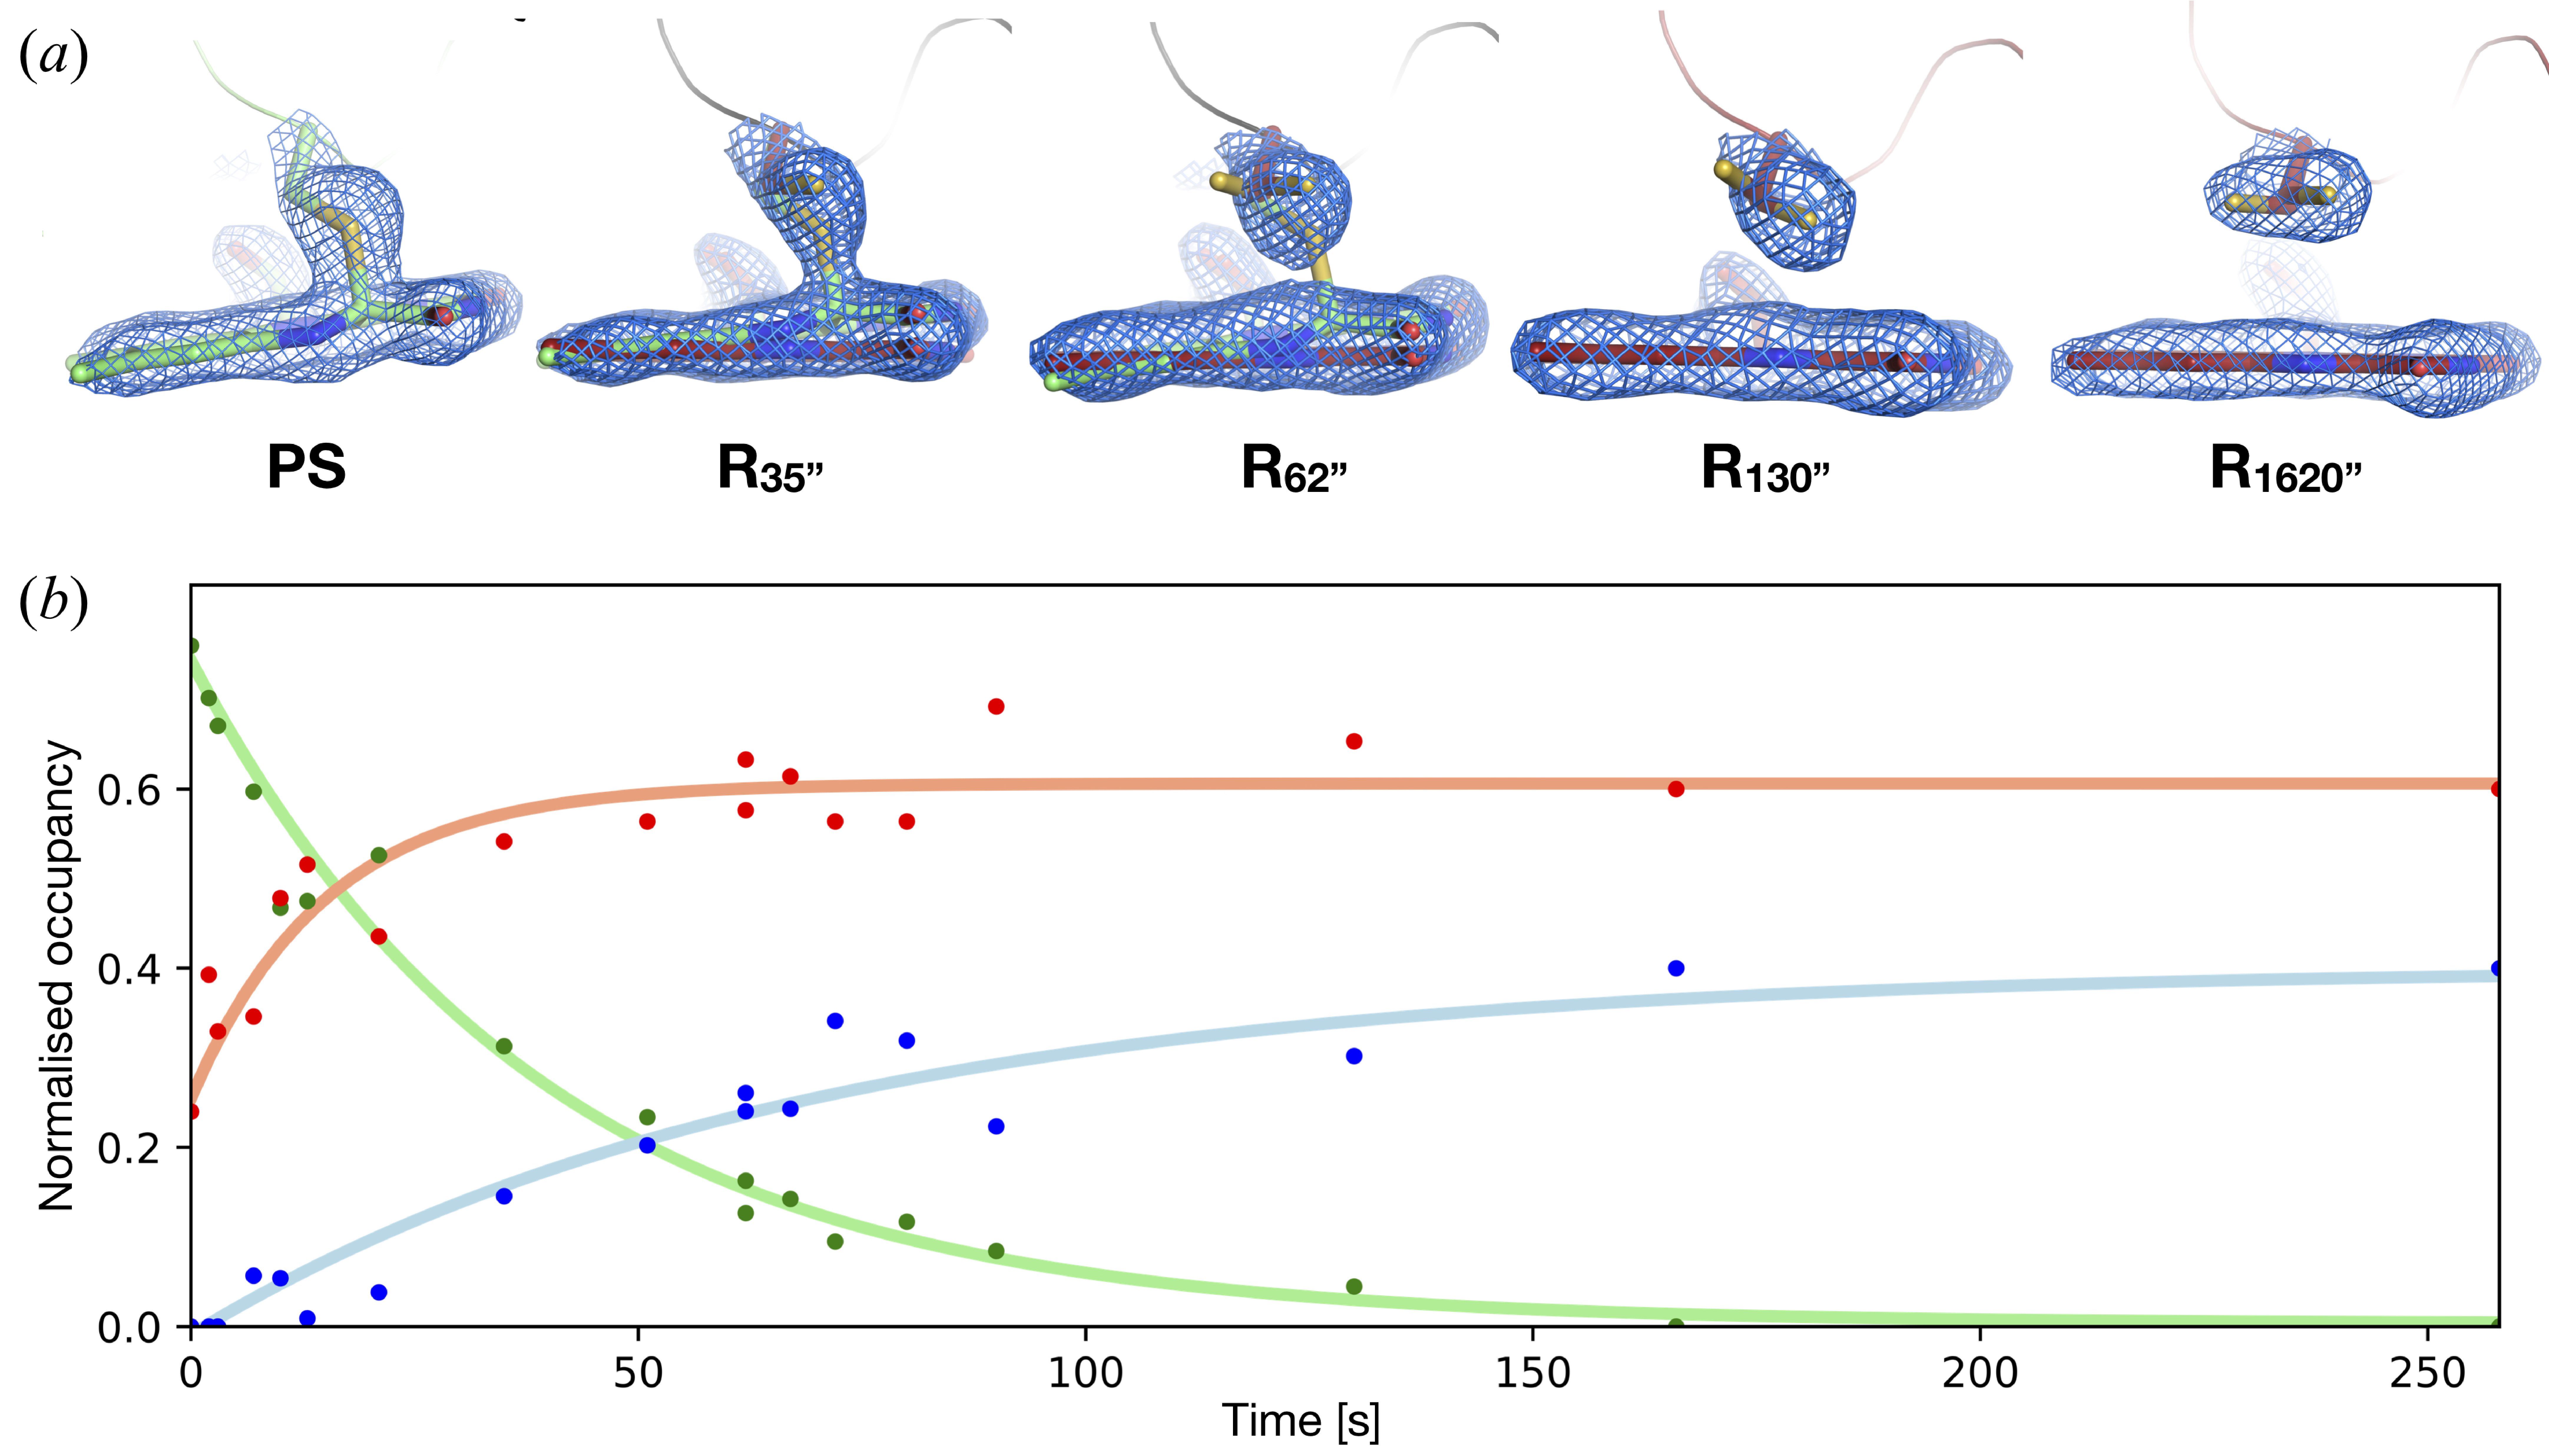
\includegraphics[width=\textwidth]{images/LOV2/LOV2slow_Fig7.pdf}
    % \hfill
    \caption{Relaxation of the photoadduct in LOV2 monitored by time-resolved crystallography. (\textit{a}) Evolution of the 2\textit{F}\textsubscript{obs} – \textit{F}\textsubscript{calc} electron density map contoured at a 1.5 \textsigma level superimposed on the C426 and the FMN chromophore at selected time points between the PS equilibrium (t < 0 s) and 1620 s (L-state in green, D''-state in firebrick). (\textit{b}) Occupancy evolution over time of the three conformations of C426 showing the progressive disappearance of the photoadduct (conformation C: green) and the appearance of the two ground state conformations (major conformation A: orange, minor conformation B: blue).}
    \label{fig:LOV2slowphotoadductdecay}
\end{figure}

The 18 datasets were obtained from distinct locations of six different crystals. The build up of the PS equilibrium in each of these crystals led to variable combinations of L-state/D'-state occupancies. As a consequence, in order to be able to plot the time evolution of occupancies during relaxation, respective occupancies were normalized with respect to the L-state/D0state occupancies in the PS equilibrium of the crystal on which a given time point was recorded. The occupancy evolution of the various conformations of C426 (A: major conformation in the ground state; B: minor conformation in the ground state; C: photoadduct conformation in the L-state) is plotted in Fig. \ref{fig:LOV2slowphotoadductdecay}(\textit{b}). The decay of the C conformation, modelled as an exponential, occurs with a time constant of 39 s, which is in very good agreement with the time constant derived by \textit{ic}AS (39.6 and 39.7 s for two different time series). The rise of the A conformation occurs significantly faster (time constant of 15 s), which may sound counterintuitive, but can be explained by a rapid plateauing to its maximum occupancy in the ground state, while the appearance of the B conformation slowly develops (time constant of 67 s) and ends up fully compensating the final disappearance of conformer C.

\subsubsection{C-terminus reordering}
The C-terminus is perfectly ordered up to residue L502 in the dark state D [Fig. \ref{fig:LOV2slowdiffstates}(\textit{e}), Fig. S2, start of photocycle in Fig. \ref{fig:LOV2slowicphotocycle}(\textit{a})]. It is then fully disordered in the PS equilibrium starting from residue I495, which applies to both the dark state D0 and the L-state, [Fig. \ref{fig:LOV2slowdiffstates}(\textit{e}), PS step of photocycle in Fig. \ref{fig:LOV2slowicphotocycle}(\textit{a})]. When determining the structures corresponding to the various R\textsubscript{xxxx''}, we already observed the progressive reappearance of electron density on the C-terminus in the early time points, \textit{i.e.} before the crystal phase transition [R6200 snapshot of photocycle in Fig. \ref{fig:LOV2slowicphotocycle}(\textit{a})]. However, immediately after the transition and the loss of a crystal symmetry element, while one monomer shows an increased level of electron density on the C-terminus (monomer A), the second monomer (monomer B) hardly shows any [R\textsubscript{130''} snapshot of photocycle in Fig. \ref{fig:LOV2slowicphotocycle}(\textit{a})]. Coincidentally, the conformation of the C-terminus in the former monomer is that of the \textalpha-helical one, and in the latter, of the hook-shaped one. Fig. \ref{fig:LOV2slowicphotocycle}(\textit{b}) indirectly illustrates the disordering/reordering of the C-termini by plotting the average \textit{B}-factor of residues 493 to 495, normalized by the average \textit{B}-factor of the whole structure. The electron density for monomer B only reappears significantly in snapshot R\textsubscript{1620''} [Figs. 8(\textit{a}) and 8(\textit{b})]. This is in stark contrast with the behaviour of the C-terminus in monomer A which settles before 100'' [Fig. \ref{fig:LOV2slowicphotocycle}(\textit{b})].
\newline The comparison of the C-terminus structure of both monomers allowed us to identify the conformation of the W467 side chain as a key determinant of their respective \textalpha-helical or hook-shaped conformations. In the D''-state, this side chain adopts in monomer A the conformation observed in the D-state (conformation W467-A) whereas in monomer B, it adopts a markedly different conformation, W467-B, where the indole ring is essentially displaced by a \textasciitilde 90\degree  rotation around the C\textalpha—C\textbeta  bond (Fig. S6). In fact, the two conformations are mutually exclusive, i.e. one conformation of the side chain sterically prevents stabilization of the opposite C-terminus conformation. Fig. \ref{fig:LOV2slowicphotocycle}(\textit{c}) illustrates the reorientation of the W467 side chain by plotting its average B-factor, normalized by the average B-factor of the whole structure. The curves are very similar at early time points but markedly diverge after 70 s. Indeed, W467 has one single conformation at the beginning of the photocycle, which is maintained in monomer A after the phase transition [Fig. \ref{fig:LOV2slowicphotocycle}(\textit{a})]. Conversely, the side chain of W467 in monomer B adopts a dynamic equilibrium between 70 and 130 s, which resolves into the single conformation W467-B from then on. Coincidentally, the (70–130 s) time range corresponds to the time period when the percentage of spots initially indexed in space group \textit{P}4\textsubscript{3}2\textsubscript{1}2 to \textit{P}2\textsubscript{1}2\textsubscript{1}2\textsubscript{1} hovers around 50\% (Fig. \ref{fig:LOV2slowindexP4}).
\subsubsection{Resetting the photocycle}
The \textit{\textit{in crystallo}} photocycle described above may appear non-reversible, at least on the timescales we probed (<30 min), since its endpoint D'' differs from its starting point D by the conformation of the C-terminus in half the molecules of the crystal. However, we discovered that, by illuminating a crystal in the D''-state (i.e. in the space group \textit{P}2\textsubscript{1}2\textsubscript{1}2\textsubscript{1}), we could restore the PS equilibrium in the space group \textit{P}4\textsubscript{3}2\textsubscript{1}2 to \textit{P}2\textsubscript{1}2\textsubscript{1}2\textsubscript{1} (Fig. \ref{fig:LOV2slowindexP4}), bypassing the D-state, and thus reset the photocycle leading to photoadduct relaxation, C-terminus reordering and W467 side-chain reorientation [Fig. \ref{fig:LOV2slowicphotocycle}(\textit{a})].
\begin{figure}[H] %bt!]
    \centering
    \noindent \includegraphics[width=0.8\textwidth]{images/LOV2/LOV2slow_Fig8.pdf}
    \hfill
    \caption{Observation of slow protein dynamics in LOV2 leading to complex C-terminus reordering concomitant with loss of crystal symmetry. (\textit{a}) Structural description of the events occurring to the LOV2 C-terminus along the illumination sequence described in Fig. \ref{fig:LOV2slowexpscheme}(\textit{b}). The 2\textit{F}\textsubscript{obs} - \textit{F}\textsubscript{calc} electron density map contoured at a 1.5\textsigma level is superimposed on the C-terminus (residues 491 to 503) and residue W467 for the ground state, then at selected time points between the between the PS equilibrium (t < 0 s) and 1620 s. The C-terminus is ordered in the D-state, disorders in the PS equilibrium, then progressively reorders until a crystal phase transition at \textasciitilde70 s, at which point each monomer in the asymmetric unit of the new space group orders dissimilarly. One monomer quickly reorders as in the D-state, and the other orders more slowly to a distinct, hook-shaped conformation. The phase transition is governed by flipping of a conserved tryptophan residue positioned in the vicinity of the C-terminus. The resulting photocycle cannot proceed back to the D-state (red cross) but can be reset by re-illumination. (\textit{b}) Illustration of C-terminus disordering/ordering by monitoring of the normalized B-factor of the stretch of residues 493 to 495 for monomer A (\textalpha-helical C-terminus) in orange, and for monomer B (hook-shaped C-terminus) in blue. (\textit{c}) Corresponding evolution of the normalized B-factor of W467, suggesting a rationale for space group transition.}
    \label{fig:LOV2slowicphotocycle}
\end{figure}

\section{Discussion}\label{sec:slowprot_discussion}
In this study, we coupled RT spectroscopy and crystallography to probe the slow protein dynamics occurring on the time scale of tens of seconds to tens of minutes, involved in the relaxation of a blue-light-induced photoadduct in LOV2. \textit{in crystallo}, we could visualize the decay of the photoadduct population following the release of the PS equilibrium, elucidating, under our experimental conditions (crystalline state, composition of the mother liquor, temperature, humidity), a decay time constant of \textasciitilde40 s. In addition to this expected result, we observed an unanticipated phase transition, which occurs 70 to 80 s after the release of the PS equilibrium. This phase transition consists of the loss of a crystal symmetry element, which corresponds to the transition of the asymmetric unit from a monomer in the tetragonal space group \textit{P}4\textsubscript{3}2\textsubscript{1}2 to \textit{P}2\textsubscript{1}2\textsubscript{1}2\textsubscript{1} to a dimer in the orthorhombic space group \textit{P}2\textsubscript{1}2\textsubscript{1}2\textsubscript{1}. The non-crystallographic dimer is obtained from a crystallographic dimer whose molecules have slid apart. The C-terminus of the protein is fully disordered in the PS equilibrium, then progressively reorders to its \textalpha-helical conformation. After the phase transition, the continuation of the ordering of the C-termini develops asymmetrically into distinct conformations and at different rates. While monomer A continues to fold in the \textalpha-helical conformation, which is completed within 130 s, monomer B refolds at a slower rate into a very different, hook-shaped conformation, which appears to be fully completed only after 1620 s. The difference in C-terminus conformation is coupled to the orientation of the side chain of a nearby bulky residue, W467, which rotates by \textasciitilde90\degree in order to accommodate the hook-shaped conformation of the C-terminus.
\newline
The formation of the photoadduct in the PS equilibrium drives the tilt of the isoalloxazine ring of the chromophore, inducing a reorganization of surrounding side chains, which eventually leads to the destabilization of the C-terminus. The release of the PS equilibrium allows the FMN and Q489 to retrieve their original orientation, and residues 489 to 491 to re-stabilize, which then sets up the conditions for C-terminus reordering. The structural origin for the crystal phase transition cannot be definitively ascertained, but the crystal packing analysis of the D-state structure [Fig. \ref{fig:LOV2slowSGswitch}(\textit{a})] reveals a large network of electrostatic interactions between three symmetry-related LOV2 molecules involving eleven charge-bearing residues (seven arginines, one glutamate, four aspartates), two uncharged polar residues (two glutamines) and the negative charges of the phosphate groups of two FMN molecules. The network of interactions is reorganized in the L-state structure upon the formation of the photoadduct: the movement of the isoalloxazine ring pulls the C426 side chain, which in turn pulls the R426 side chain [straight green arrow in Fig. \ref{fig:LOV2slowSGswitch}(\textit{b})]. Concomitantly, there are rotations of both phosphate groups [circular arrows in Fig. \ref{fig:LOV2slowSGswitch}(\textit{b})]. Relaxation of the photoadduct induces another reorganization of the network of charges [Fig.9(\textit{c})], eventually leading to the breakage of a salt bridge between R424 and E433 belonging to two different LOV2 molecules, which constitutes a key crystal contact in both the D-state and the PS equilibrium in slightly different orientations [dashed line in Figs. 9(\textit{a}) and 9(\textit{b})]. The loss of this salt bridge may drive the sliding motion associated with the phase transition. Besides, the rotation of both phosphate groups directly influences the position of adjacent residues R427 and R443 altering the charged network around R447 from a symmetry-related LOV2 molecule, thus affecting another crystal contact. Therefore, we propose that the release of crystal contacts associated with the relaxation of the photoadduct induces an asymmetric reorganization of this network of electrostatic interactions, which then drives the sliding motion of the two molecules relative to each other and thus fuels the space group change. As a consequence, the refolding volume available to the C-terminus of each of the two monomers is different, creating possibilities for new types of interactions with neighbouring residues. Most importantly, we observe that residue W467, which belongs to a well-conserved FWN sequence of residues found in LOV domains (Fig. S7), acts as a gate discriminating between the two conformations of the C-terminus.
\begin{figure}[H] %bt!]
    \centering
    \noindent 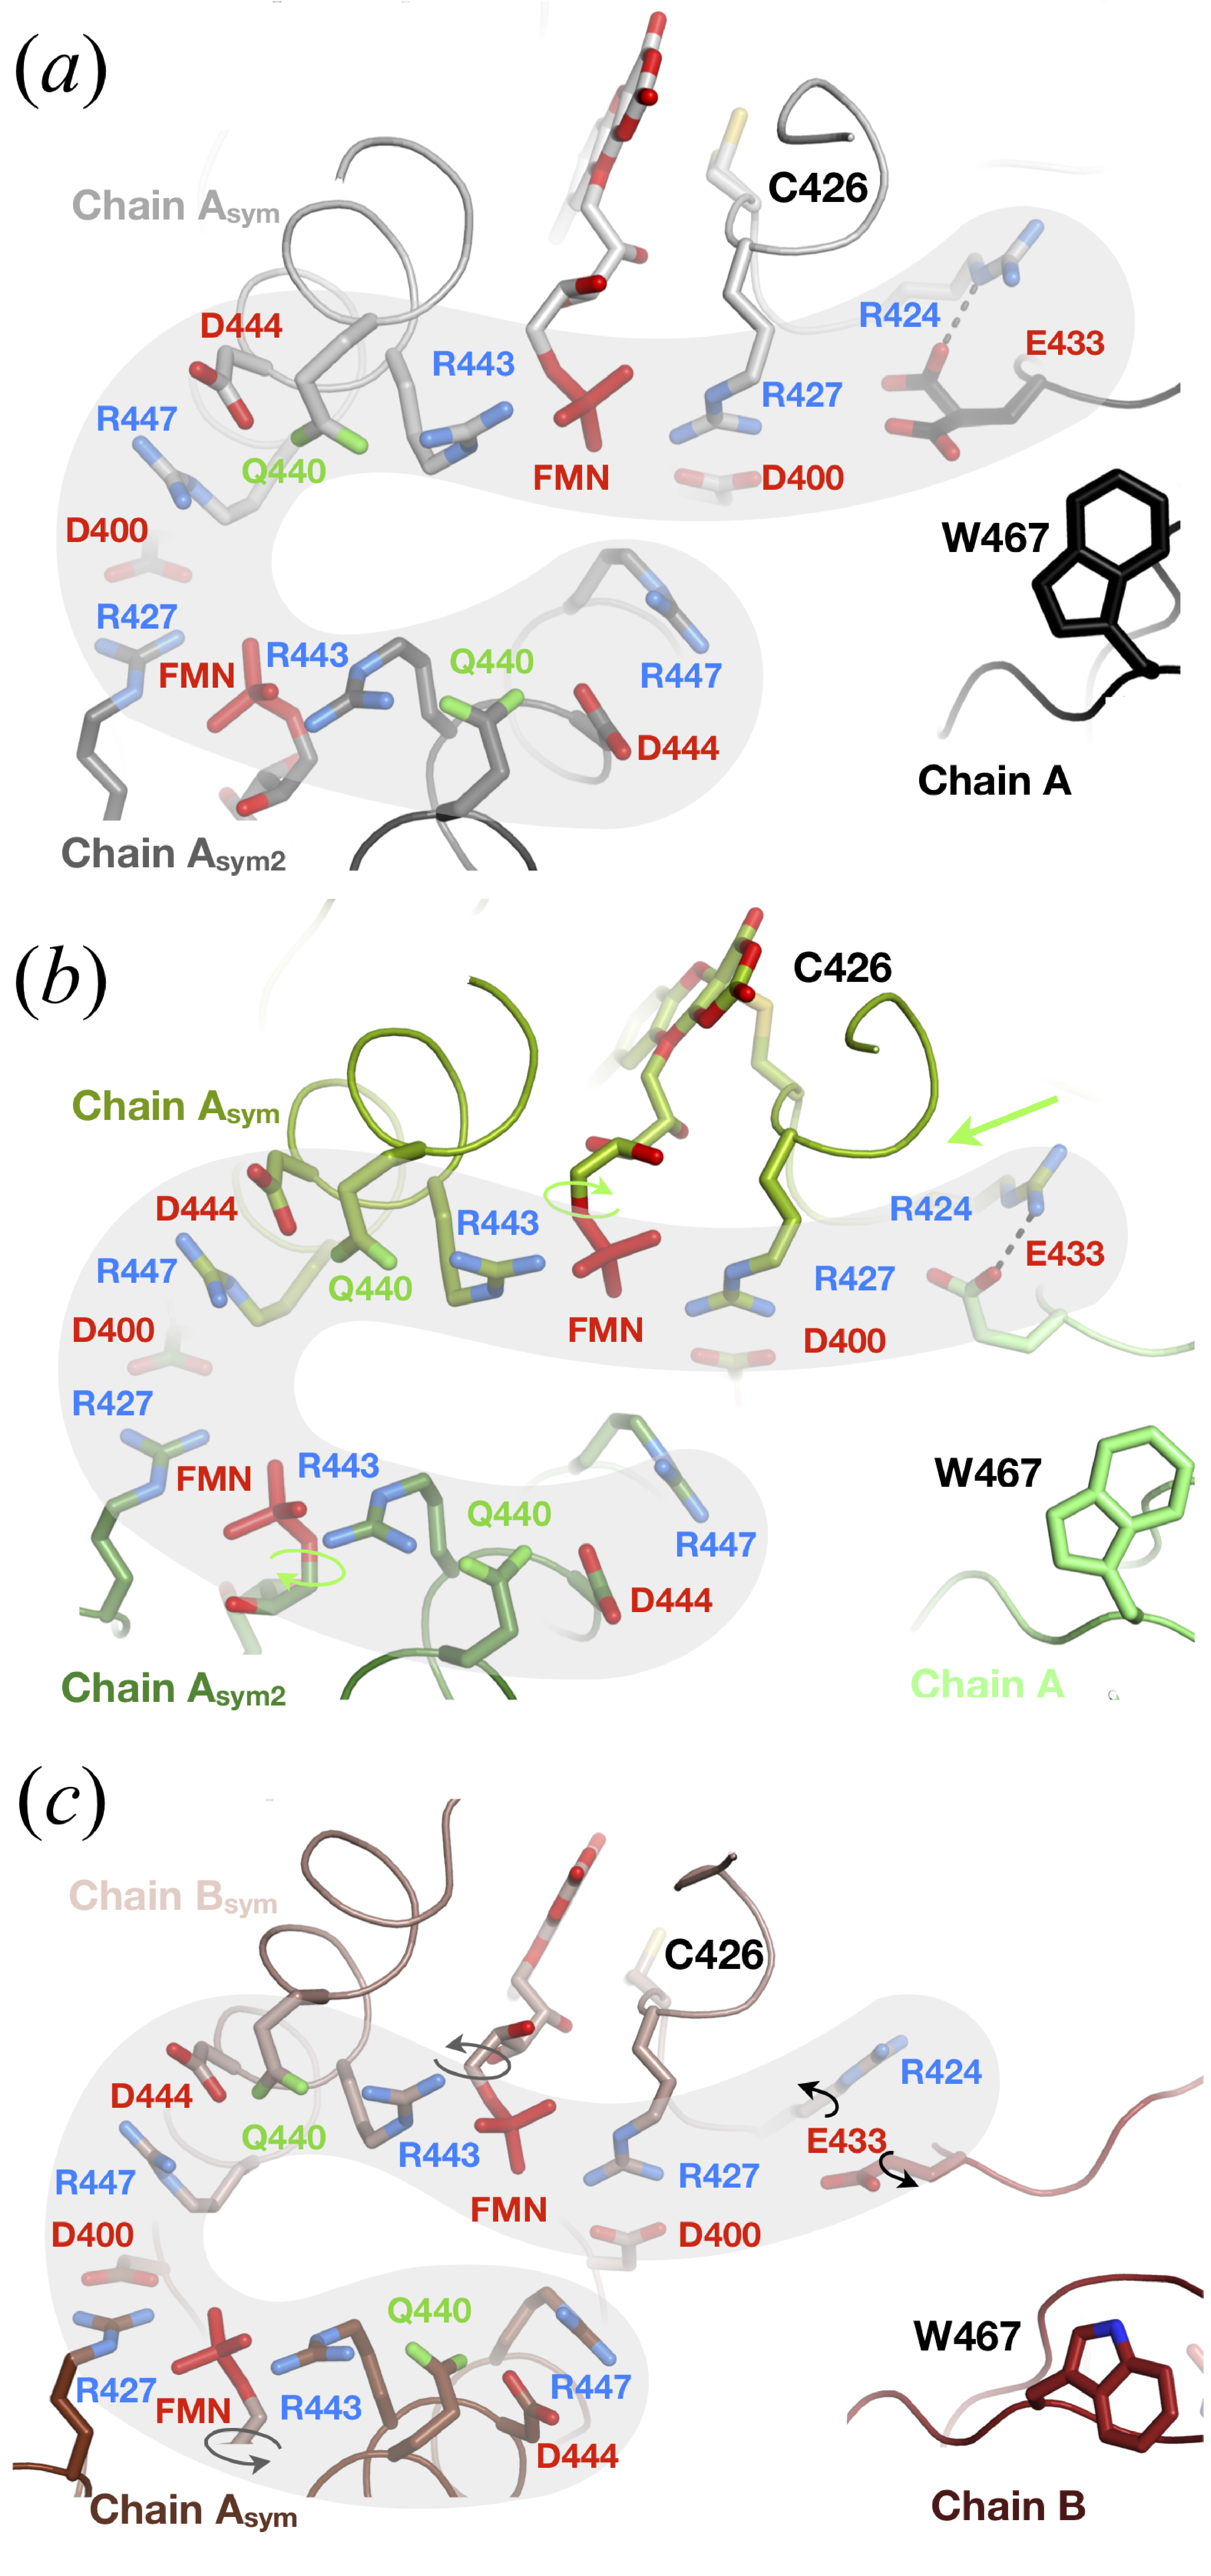
\includegraphics[width=0.6\textwidth]{images/LOV2/LOV2slow_Fig9.pdf}
    \hfill
    \caption{Effect of photoadduct relaxation on the electrostatic network connecting symmetry-related chains. (\textit{a}) The D-state structure is displayed as a black ribbon, and the symmetry-related molecules Asym and Asym2 as light-grey and dark-grey ribbons. (\textit{b}) The L-state structure is displayed as a green ribbon, and the symmetry-related molecules Asym and Asym2 as split-pea and forest-coloured ribbons. (\textit{c}) The D''-state structure is depicted as a firebrick ribbon and the symmetry-related molecules Asym and Bsym as dark salmon and chocolate, respectively. Negatively and positively charged residues are depicted in red and blue, respectively, and key residues are represented as sticks. The black dashed line highlights the presence of a salt bridge in the D-state and L-state structures.}
    \label{fig:LOV2slowSGswitch}
\end{figure}
In brief, we observed the appearance of a symmetry-breaking phenomenon during the \textit{in crystallo} relaxation of the LOV2 photoadduct. This is likely not physiologically relevant to this specific LOV domain, as AtPhot2LOV2 has been decisively shown to be monomeric \parencite{katsuraOligomericStructureLOV2009, nakasakoDomainOrganizationPlant2020} and is thus a probable artefact of the crystal packing that creates non-physiological networks between charged residues and cofactors. However, we cannot exclude that the resulting asymmetric dimer resembles a physiological homodimer or heterodimer formed between other LOV domains. Indeed, the differential C-terminus reordering in the two molecules of a given dimer is reminiscent of a cooperative interaction. Such a cooperative interaction has been described in a heterodimer formed by LOV1 and LOV2 domains within phototropin 2 from \textit{Arabidopsis thaliana}, involved in photoadduct half-life modulation \parencite{kasaharaPhotochemicalPropertiesFlavin2002} and in the conformational changes that lead to J\textalpha-helix unfolding and kinase domain activation \parencite{oideBlueLightExcited2018}. The fact that W467 belongs to a highly conserved short motif can only support this hypothesis.


\subsection{Modelling Phototropin II to assess allostery}\label{sec:PhotII_AF}
This is an extension of the work carried out in \cite{aumonierSlowProteinDynamics2022}, in which the physiological relevance of the asymmetric dimer is tentatively assessed. 

The systematic nature of the space group change over the entire crystal hints at a potential 'allostery-like' action of one monomer over the other in the F'' dimer. Further, it is the flip of a very conserved tryptophan residue, as well as a concentration of charges from the vicinity of both FMN molecules that prevent one C-terminus from properly refolding. The full-length Phototropin II comprises two LOV domains, which are packed against each other in the folded protein, and form an 'auto-dimer' in the full-length Phototropin II \parencite{oideBlueLightExcited2018}. The systematic action of one monomer over the other in D'' could replicate a physiological allosteric effect of LOV1 over LOV2, which has been documented \parencite{kasaharaPhotochemicalPropertiesFlavin2002}, but the current state of the literature does not allow us to confirm whether the crystal packing form obtained with our constructs replicates the interactions between LOV1 and LOV2.

To answer this question, we inspected the \textit{in sillico} model of Phototropin II from \textit{Arabidopsis thaliana }as modelled by AlphaFold 2 \parencite{jumperHighlyAccurateProtein2021} in the European Bioinformatics Institute (EBI) modelled protein database \parencite{varadiAlphaFoldProteinStructure2022}. The second LOV domain (blue, J\textalpha in marine) of the full-length phototropin II of \textit{Arabidopsis thaliana} (green), was aligned with the chain A of the asymmetric dimer of D'' (red). AlphaFold models Phototropin II with reasonable confidence, especially the LOV1 (residues 117:246) and LOV2 (residues 389:504) domains (Fig. \ref{fig:PhotII_AF2} (b)). 

The interface between both monomers in D'' does not match the predicted interface between the two LOV domains in the modelled full-length phototropin II \footnote{This is also true for each symmetry mates of any of the monomer of the D'' dimer.}. In particular, the folding of the C-terminal segment of the LOV2 construct (folded towards the foreground) used in this study does not match the position of the J\textalpha\ helix of the LOV2 domain from the full-length phototropin II (folded towards the background). Hence, it is unlikely that the action of chain A on chain B observed in D'' during this study has physiological relevance, and more likely that it is a crystallographic artefact \footnote{The modelling confidence at the region of the interface is high, allowing to conclude, even from a model. Of course, experimental validation would be needed, but there are currently no experimental structures of the full-length Phototropin II.}. 

\begin{figure}[H] %bt!]
    \centering
    \noindent \includegraphics[width=\textwidth]{images/LOV2/PhotII_struc.pdf}
    \hfill
    \caption{Modeling of the full-length Phototropin II from \textit{Arabidopsis thaliana}, compared with the D'' dimer. (a) Phototropin II (green) from the EBI modelled protein database from AlphaFold2, with its second LOV domain (LOV2, blue, J\textalpha\ helix in marine) aligned on the chain A of the D'' structure (red). The low confidence (<70 \%) regions have been coloured orange and the first LOV domain is coloured in purple, with its C-terminal J\textalpha\ helix in pink. The rest of the phototropin is coloured green. The D'' dimer (chain A and chain B) is coloured in red. (b) Error matrix of the prediction, showing  the LOV1 (residues 117:246) and LOV2 (residues 389:504) domains as the most confidently predicted regions.}\label{fig:PhotII_AF2}
\end{figure}

\section{Conclusion}

Our study demonstrates the feasibility of monitoring the progress of protein conformational changes at room temperature on timescales that can be considered ‘slow’, from seconds to tens of minutes, using relatively recently developed X-ray crystallography instruments (fast hybrid photon-counting detectors, sample humidity control device). Though our time-resolved approach is based on the quasi-instantaneous activation by light of a photosensitive protein, it can be extended to slower triggers such as ligand diffusion or change in physicochemical parameters (temperature, pH, ionic strength, humidity). The experiments can be carried out using crystals of any size because the timescale of monitoring (seconds to minutes) can be adjusted to well above the timescale of triggering (milliseconds to seconds). One crucial requirement guiding the choice of the biological system is the capacity of the crystalline order to withstand significant structural changes during the time frame of the phenomenon studied. This methodology should greatly expand the prospects of RT crystallography, which comes at a time when X-ray crystallography will, amid the surge of cryoelectron microscopy and deep-learning-based structure prediction tools, likely become more focused on macromolecular dynamics.

\chapter{Serial Crystallography experiment to assess the unfolding the C-terminus of LOV2}\label{chap:SSX_LOV2}

LOV2 can be activated by blue light (447-430 nm), is light sensitive and its reaction to light has been structurally characterised \parencite{aumonierMillisecondTimeresolvedSerial2020}, Additionally, LOV2 microcrystal can be produced with the method described in Section \ref{sec:microcrystallisation}. For all these reasons LOV2 has been used for the commissioning of a TR-SSX setup elaborated by Shibom Basu (European Molecular Biology Laboratory, EMBL). Briefly, a  a laser-driven white light source, which is monochromated using filters was mounted so that it is focussed through the lens of the On-Axis View (OAV) objective of beamline ID23-2 at the ESRF \parencite{nanaoID232AutomatedHighperformance2022}, producing a focal spot of \(42 \times 52 \mu m\) (knife edge scan) with 10 \textmu W at the sample position. This setup aims to introduce fixed-target TR-MX capabilities on ID23-2. The beamline is especially suited to that with a \(4\times4 \mu m\) beam and high flux (\(1.8 \times 10^{13}\) photons/seconds). 

The synchronization of the laser shutter with the micro-diffractometer (MD), detector and motors of the beamline had not been implemented yet at the time of the experiment. Thus, only a ground state dataset (dark-SSX) and one where the crystals were illuminated continuously during X-ray exposure (light-SSX) could be collected as proof of the principle of the setup. LOV2 crystals of \(20 \times 20 \mu m\) were loaded onto an SOS chip \parencite{doakCrystallographyChipChip2018} and data were collected using the no-oscillation MeshScan scheme. Owing to the greater size of the laser focal spot, crystals are illuminated before they are exposed to the X-ray beam. The estimated total illumination (at 450 nm) duration for the steady-dataset is \textasciitilde 38 ms, including the X-ray exposure time. A single MeshScan was enough to yield a reasonably complete (> 10 000 indexed images) dataset, both the dark and steady 6ms dataset diffracted to a resolution of 2.2 \AA. 

The strongest feature in an Isomorphous \(F_{obs}(light\mbox{-}ssx) - F_{obs}(dark\mbox{-}ssx)\) is the positive peak corresponding to the thioether bond formed in the photoadduct state, closely followed by the negative difference electron density peaks corresponding to the recruitment of the C426 into the bond (Fig. \ref{fig:SSX} (a)). A negative peak under the C4a atom of the FMN indicates that it is no longer planar, similar to what is observed in a long-illumination steady-state (Fig. \ref{fig:LOV2slowdiffstates} (c)). The presence of the photoadduct of LOV2 after 38 ms of illumination is expected, as it is estimated to occur in the \textmu s range after excitation of the FMN \parencite{pfeiferTimeResolvedFourierTransform2009}. The refined occupancy of the activated state is \textasciitilde 80 \% using the method described in \ref{sec:LOV2_slow_occupancy}. However, the conformation adopted by Q489 in light-SSX seems like an intermediate state between its position in dark-SSX (green) and its stabilised steady-state position (green in Fig. \ref{fig:LOV2slowQ489mech}). Accordingly, the strand carrying Q489 has started to back away from the FMN but has not reached the position visible in green in Fig. \ref{fig:LOV2slowQ489mech} either. As the strand carrying Q489 has not fully buckled, the C-terminus of LOV2 in light-SSX (Fig. \ref{fig:SSX} (c)) is still in the same conformation as it is in the dark-SSX (Fig. \ref{fig:SSX} (b)), albeit with less defined electron density. The steady-state position of the C-terminus (green in Fig. \ref{fig:LOV2slowicphotocycle}) has not been reached after 38 ms of continuous illumination, suggesting that the mechanism of its disordering could be observed via TR-SSX in the ms time domain. 
\begin{figure}[H] %bt!]
    \centering
     \includegraphics[width=\textwidth]{images/LOV2/SSX.pdf}
    \hfill
    \caption{Comparison of the dark-SSX and light-SSX datasets recorded at beamline id23-2 using the SSX fixed target scheme developed by Shibom Basu (EMBL). (a) Isomorphous \(F_{obs}(38\ ms\ steady-illuminated) - F_{obs}(dark)\) electron density difference map, cut at 3.5 \textsigma level (positive peaks in blue, negative in gold), overlaid on the dark-SSX (green) and light-SSX (red) refined atomic models. In light-SSX, the carboxamide head of Q389 has rotated 180 degrees. And the body of the side chain is tilted. (b) 2\textit{F}\textsubscript{obs} – \textit{F}\textsubscript{calc} electron density map of the dark dataset contoured at a 1.0 \textsigma level around the refined model of dark-SSX. (c) 2\textit{F}\textsubscript{obs} – \textit{F}\textsubscript{calc} electron density map of the 38 ms illuminated dataset contoured at a 1.0 \textsigma level around the refined model of dark-SSX.}
    \label{fig:SSX}
\end{figure}

After 38 ms of steady illumination, the photoadduct was already present (its occupancy was estimated to be 80\% using the method described above). To our surprise, the light-SSX did not feature the disordered C-terminus of our PS datasets. This strongly suggests that this disorganisation happens after the 38 ms time-mark. It validates that the disorganization phenomenon could be studied with this setup.

Given that the main project of this PhD is to study the structural reorganizations happening after the build-up of the photoadduct and leading to the disorganization of the C-terminal \textalpha\ helix of LOV2, any methodological or biological knowledge acquired on this construct can be used to further the main project of this PhD.





}

\pagebreak

\part{Study of a Class II CPD Photolyase and a bifunctional cryptochrome}\label{part:Photolyase-Cryptochromes}

	{\section{The Photolyase Cryptochrome superfamily}\label{sec:PCSF}
Photolyases and cryptochrome are evolutionarily linked flavoproteins \parencite{conradPhotochemistryFlavoproteinLight2014}. Photolyases harvest light to repair DNA damage \parencite{sancarMechanismsDNARepair2016}. Cryptochromes were originally discovered to be blue light sensors regulating a vast array of functions \parencite{ahmadHY4GeneThaliana1993}, they are present both in plants and animals \parencite{meiEvolutionaryHistoryPhotolyase2015} and have since been discovered to serve a vast array of additional functions. Most, but not all cryptochromes are blue-light sensors. Cryptochromes and photolyases share a similar bilobial architecture made of a flavin adenine dinucleotide (FAD) binding C-terminal domain (pink Fig. \ref{fig:PCSF}) as well as an N-terminal Rossman folded domain (coloured lavender in Fig. \ref{fig:PCSF}, often referred to as \textalpha-\textbeta domain), able to bind an antenna chromophore. In some cryptochromes, the C-terminal domain is also capable of binding nucleotides \parencite{franzStructureBifunctionalCryptochrome2018}. In cryptochromes, these two domains (pink and lavender coloured Fig. \ref{fig:PCSF} (b)) combined are referred to as the photolyase homology region (PHr) In addition to those, cryptochromes feature an additional C-terminal extension (coloured orange in Fig. \ref{fig:PCSF} (b)) which can be of different lengths. The length of that domain is tightly linked to the various functions exhibited by cryptochromes \parencite{chavesFunctionalEvolutionPhotolyase2006}. In particular, the C-terminus of the \textit{Arabidopsis thaliana} cryptochrome is responsible for mediating the response to blue light \parencite{kongCterminalKinaseFragment2007}. 

\begin{figure}[H]
  \centering
  \includegraphics[width=\textwidth]{images/cracry/Photolyase_Cryptochromes.pdf}
  \hfill
  \caption{Overview of the Photolyase and Cryptochrome secondary structures and photoreactions. (a) Photolyase (Class II, CPD, \textit{Methanosarcina mazei}, pdb structure 7YEO) in complex with a DNA strand bearing a CPD type lesion. The N-terminal domain Rossman fold is coloured in lavender, the C-terminal domain is pink, the flavin cofactor is coloured yellow, and the DNA strand is orange. The electron transfer chain tryptophan triad is coloured red. (b) Cryptochrome (\textit{Chlamydomonas reinhardtii}, unpublished dark structure) N-terminal and C-terminal domains as well as the flavin cofactor and tryptophan triad are coloured identically as for (a). Additionally, the extra tyrosine forming the original tetrad of this cryptochrome is coloured green, as well as its proton donor. The C-terminal \textalpha-22 helix is coloured in orange. (c) Photoreaction of a photolyase: two subsequent photoreduction and protonation events are needed for DNA damage repair (d) Photoreaction of a cryptochrome with an oxidised ground state: A first photoreduction event happens, creating the semiquinone FAD containing signalling state, sensitive to blue light. This state can be further protonated to form a neutral semiquinone, sensitive to red light.}\label{fig:PCSF}
\end{figure}

In addition to their global architecture, Photolyases and Cryptochrome base their functions on the different redox states of their flavin cofactor. The ground state of all discovered photolyases is believed to be the oxidised state, the flavin cofactor must undergo two rounds of photoreduction by blue light to be catalytically active (Fig. \ref{fig:PCSF} (c), \cite{liuDynamicsMechanismsDNA2015}). Whether the flavin cofactor of cryptochromes is oxidised or semi-reduced (semiquinone) in their ground states is still up for debate \parencite{berndtNovelPhotoreactionMechanism2007, ozturkMechanismPhotosignalingDrosophila2014}. Although the recent discovery of a cryptochrome capable of signalling from both blue light and red light \parencite{beelFlavinBindingCryptochrome2012} suggests that both the oxidised flavin-containing and the semiquinone-containing cryptochromes could be physiological ground states, serving as photoreceptors for different wavelengths \parencite{kavakliPhotolyaseCryptochromeFamily2017}. In its ground state, the cryptochrome is photoreduced once, the change of polarity of the FAD sets in motion the signalling sequence of events. The signalling state can optionally be protonated, which extends its light sensitivity to red, and extends its lifetime \parencite{lacombatUltrafastOxidationTyrosine2019}.

The FAD is buried deep within the protein in both cryptochromes and FAD. Consequently, it cannot steal an electron from the solvent after excitation by a blue light photon. Instead, it takes it from a conserved tryptophan, and the electron-hole left by that transfer gets passed along an electron transfer chain formed by a conserved triad of tryptophans (red on Fig. \ref{fig:transferchain} \cite{liuDeterminingCompleteElectron2013, lacombatUltrafastOxidationTyrosine2019}). This triad (optionally completed by a fourth tryptophan \parencite{celliniStructuralBasisRadical2022} or tyrosine \parencite{franz-badurStructuralChangesBifunctional2019}, coloured green in Fig. \ref{fig:PCSF} (b)) carries the electron-hole until a solvent-exposed region, where it can be regenerated if an electron donor is present. after the first round of photoreduction, the semiquinone FAD is protonated by a nearby amino acid (teal on Fig. \ref{fig:transferchain} ) acting as a proton donor. 
\begin{figure}[H]
  \centering
  \includegraphics[width=\textwidth]{images/cracry/transfer_chain.pdf}
  \hfill
  \caption{Schematic representation of the Electron and proton transfer events underlying the photoreduction of cryptochromes and photolyases, using the structure of the Class II CPD photolyase of \textit{Methanosarcina mazei}. Less than a ps after it has absorbed a blue light photon, the FAD cofactor (green) steals an electron from a nearby tryptophan (red, W1). Several tens of ps later, W1 steals an electron from W2, and more than a hundred ps later, W2 steals an electron from W3 (all in red). W1, W2 and W3 are highly conserved in the photolyase and cryptochrome superfamily and form the electron chain triad. On the ms time scale, a nearby amino acid optionally gives a proton to the FAD (teal). }\label{fig:transferchain}
\end{figure}
Despite their drastically different functions, cryptochromes and photolyases share the same chassis, and framework of photoreduction scheme, followed by an electron transfer chain and a potential protonation. 

\subsection{Photolyases}

Exposure to UV damages the DNA in cells. UVB (315 - 280 nm) are most prone to creating DNA lesions \parencite{oakUVSkinPhotocarcinogenesis2018}. These lesions primarily occur in pyrimidine-rich segments of the cell's genome. The most abundant type of lesion present on a DNA strand after exposure to UV is Cyclobutane Pyrimidine Dimers (CPD) \parencite{oakUVSkinPhotocarcinogenesis2018}: two adjacent pyrimidine bases (thymine or cytosine) by their C5 and C6 atoms, forming a cyclobutane structure (Fig. \ref{fig:damagetype} (a)). Pyrimidine 6-4 pyrimidone photoproducts (6-4PP) are also created by exposure to UV: the two adjacent pyrimidine bases become linked covalently by their C4 and C6 atoms (Fig. \ref{fig:damagetype} (b)). These lesions bend the DNA strand and end up causing mutations down the line via replication errors. 

\begin{figure}[H]
  \centering
  \includegraphics[width=\textwidth]{images/cracry/damagetypes.pdf}
  \hfill
  \caption{The main type of DNA lesion occurring on a DNA strand after exposure to UV. (a) Upon UV exposure, two following pyrimidine bases (here, thymine) become covalently bonded twice, by their respective C6 and C5 atoms, forming a cyclobutane pyrimidine dimer (b) Upon UV exposure, a covalent bond forms between the C6 atom of the first base and the C4 atom of the second base, forming a dimer called a 6-4 photoproduct. Reproduced from \parencite{oakUVSkinPhotocarcinogenesis2018}}\label{fig:damagetype}
\end{figure}
In humans, the mutations caused by these DNA lesions go on to be the leading cause of skin cancer \parencite{cadetUltravioletRadiationmediatedDamage2005}. Of note, humans use a complex enzymatic pathway, called nucleotide excision repair (NER) to repair DNA lesions. Most organisms use a more straightforward approach: a single protein powered by light, the photolyase, identifies and repairs the lesion. Photolyases are one of the three discovered photoenzymes, the only enzymes known to physiologically harvest light to catalyse chemical reactions \parencite{bjornPhotoenzymesRelatedTopics2018}. 

The existence of a light-powered DNA repair enzyme was first discovered in 1958 by Claud S. Rupert, when he realised that virus DNA which had been inactivated by exposure to UV radiation could be reactivated in the presence of a cell lysate of E. coli, and under visible light exposure \parencite{rupertPHOTOREACTIVATIONVITROULTRAVIOLET1958}. The enzyme responsible for this function was only later identified some 25 years later \parencite{sancarDNAPhotolyasesPhysical1990}. The first photolyase whose structure was solved with X-ray crystallography was the CPD photolyase of \textit{Escherichia coli} \parencite{parkCrystalStructureDNA1995}. The structure of a photolyase from \textit{Drosophila melanogaster}, capable of repairing 6-4PP was later solved \parencite{maulCrystalStructureMechanism2008}.

It was later determined that there were several families of CPD photolyases \parencite{meiEvolutionaryHistoryPhotolyase2015}. The \textit{E. coli} CPD photolyase previously mentioned belongs to the Class I subfamily, prevalent among prokaryotes. In Eukaryotes, the Class II CPD photolyase family is more present. The first structure of a Class II photolyase solved was that of \textit{Methanosarcina mazei} \parencite{kiontkeCrystalStructuresArchaeal2011}, revealing a more compact fold. A third subclass of photolyases was more recently identified \parencite{ozturkPurificationCharacterizationType2008}.

It is nowadays accepted that the common ancestor to the photolyase-cryptochrome superfamily was likely a Class I CPD photolyase \parencite{mullerStructuralBiologyDNA2009}. 

\subsection{Cryptochromes}\label{sec:cryptochrome_families}
Cryptochromes owe their cryptic name to the vast array of functions that they perform, their ubiquitous nature and the lack of knowledge of their mechanism. In 1993, a gene was identified as responsible for the elongation of the hypocotyl as a response to blue light in \textit{Arabidopsis thaliana} \parencite{ahmadHY4GeneThaliana1993}. It was later discovered that this gene encoded the first ever discovered blue-light sensor of plants, the cryptochrome. Cryptochromes were also identified in other plants, as responsible for flowering, as well as a variety of other functions\parencite{kavakliPhotolyaseCryptochromeFamily2017}. This already vast set of functions was extended by the discovery of cryptochromes in \textit{Drosophila melanogaster}, as photoreceptors regulating the circadian clock \parencite{emeryCRYDrosophilaClock1998,stanewskyCrybMutationIdentifies1998}. Mammals also feature cryptochromes, involved in the circadian clock \parencite{vitaternaDifferentialRegulationMammalian1999}. 

Animal cryptochromes (such as that of \textit{Drosophila melanogaster} share a strong homology with 6-4 photolyases, while plant cryptochromes are closer to Class I CPD photolyases \parencite{kavakliPhotolyaseCryptochromeFamily2017}. As a consequence, cryptochrome feature C-terminal domains (coloured orange on Fig. \ref{fig:PCSF} (b)) of extremely variable length (3 to 300 amino-acid long), which appear to be tightly linked to their function \parencite{partchRoleStructuralPlasticity2005}. This strong variability allows different cryptochromes to interact with different partner proteins, partially explaining how they can regulate seemingly unrelated functions \parencite{meiEvolutionaryHistoryPhotolyase2015}. A family of cryptochromes deprived of C-terminal (CRY-DASH, for \textit{Drosophila}, \textit{Arabidopsis}, \textit{Synechocystis}, and \textit{Homo}) domain was also identified \parencite{brudlerIdentificationNewCryptochrome2003}. Members of this family originate from a CPD photolyase, as is the case for plant cryptochromes, despite CRY-DASH being also present in animals \parencite{chavesCryptochromesBlueLight2011}. CRY-DASH cryptochromes have retained their ability to repair CPD DNA lesions, but only on single-strand DNA, and no longer on double-stranded DNA \parencite{selbyCryptochromePhotolyaseClass2006}. 

Many organisms possess several cryptochromes, as is the case for \textit{Arabidopsis thaliana} which possesses two plant-like cryptochromes (CRY1 and CRY2), and a CRY-DASH (CRY3) \parencite{kavakliPhotolyaseCryptochromeFamily2017}. Accordingly, a unique type of animal-like cryptochrome (animal-like cryptochrome) was more recently discovered in \textit{Chlamydomonas reinhardtii}, despite \textit{Chlamydomonas reinhardtii} already having a plant-like cryptochrome and two CRY-DASH \parencite{beelFlavinBindingCryptochrome2012}. CraCRY is sensitive to both blue and red light and has retained its 6-4PP repair function \parencite{franzStructureBifunctionalCryptochrome2018}. 

\chapter{The mechanism of DNA repair by the Class II CPD photolyase of \textit{Methanosarcina mazei}}\label{chap:MmCPDII}

\vspace{10mm}

\section{Studying photolyases with XFEL radiation}

Despite their fame as the first characterised photoenzyme and the number of crystal structures already determined \parencite{mullerStructuralBiologyDNA2009}, the mechanism of DNA repair by photolyases had not - until very recently \parencite{maestre-reynaVisualizingDNARepair2023a, christouTimeresolvedCrystallographyCaptures2023a}, been investigated with TR-MX. This is perhaps partially explained by their extreme sensibility to specific radiation damage in the form of photoreduction of the flavin by the X-ray beam \parencite{kortDNAApophotolyaseAnacystis2004}, which can go as far as eliciting DNA repair \parencite{meesCrystalStructurePhotolyase2004}.  This is why the study of DNA repair by photolyases is only achievable using the TR-SFX technique at an XFEL, where damage-free structures can be obtained. 

\section{Visualizing the DNA Repair Process by a Photolyase at Atomic Resolution.}\label{sec:prior_MmCPDII}
Only the scope, context and results of our DNA repair paper are summarised here. The unformatted version of the full paper is available in the Supplementary Material of this manuscript (supplementary material, Chapter \ref{sec:paperMmCPDII}).

The first step of the DNA repair mechanisms is photoreduction (Fig. \ref{fig:PCSF} (c)). Photoreduction of the Class II photolyase of \textit{Methanosarcina mazei} (\textit{Mm}CPDII) has been investigated by the collaboration network previously mentioned, before the beginning of this PhD \parencite{maestre-reynaSerialCrystallographyCaptures2022}, bringing the FAD cofactor of the photolyase to the fully reduced  FADH\textsuperscript{-} state. Once the photoreduction is over, DNA repair is possible upon an additional excitation, transiently bringing the FAD to the FADH\textsuperscript{•-}, which causes an electron to be transfered to the CPD. 

Based on extensive ultrafast spectroscopy studies \parencite{zhangPhotolyaseDynamicsElectrontransfer2017}, a mechanism for the repair of CPD has been proposed: First, a forward electron transfer from the reduced cofactor FADH\textsuperscript{-} produces the CPD radical anion (T<>T)\textsuperscript{•-}, where the excess electron may be shared between the two pyrimidines. The \(C5-C5'\) of the CPD is then cleaved first, producing (T\_T)\textsuperscript{•-}. after that is the \(C6-C6'\) bond cleaved too (this step is visible in visible on Fig. \ref{fig:DNArepair_schem} (b)), yielding (T+T)\textsuperscript{•-}. Finally, there is a transfer of one electron from the anionic radical thymine, back to the FAD cofactor, regenerating the FADH\textsuperscript{-} state and neutral thymine. One of the goals of this study was to catch these spectroscopic reaction intermediates to understand how the active site of the photolyase stabilises them. 

These intermediates were investigated via a time series from 100 ps to 10 ns time-domain (100, 250, 450, 650 ps; 1, 2, 3.35, 6, 10 ns), collected with a pump-probe scheme using the pulse of a fs laser as the pump on beamline ALVRA at SwissFEL.

Even bearing a CPD lesion, a double strand of DNA retains an interaction between adenosines and thymines pairs of opposing strands in the damaged region: the CPD lesion is still within the double stranded helix \parencite{parkCrystalStructureDNA2002} It is only when the strand is paired with a CPD photolyase that the CPD region flips out of double-stranded conformation to lodge within a specific groove (visible in Fig. \ref{fig:DNArepair_schem} (a), \cite{maestre-reynaTwistTurnRevised2018}). The mechanism underlying the transition from that regionally single-stranded repaired set of based to an annealed and freed-out double strand of DNA is unknown (the isomorphous \(F_{obs}(repaired\ bases) - F_{obs}(dark)\) map for lesion repair is represented over the ground state model in Fig. \ref{fig:DNArepair_schem} (b)). This is especially interesting as the photolyase has a much lower affinity for repaired DNA, indicating that it can recognise the lesion specifically, and kicks it out once the repair is over. That last step is visible in Fig. \ref{fig:DNArepair_schem} (c).

This unknown conformational mechanism was investigated by a second pump-probe time series spanning from 10 ns to 200 \textmu s (10, 100, 500 ns; 25, 200 \textmu s), collected at SACLA where the pump was the pulse of a ns laser.

\begin{figure}[H]
  \centering
  \includegraphics[width=\textwidth]{images/cracry/Science2023.pdf}
  \hfill
  \caption{Schematic representation of the reaction visualised via TR-SFX in \cite{maestre-reynaVisualizingDNARepair2023a}. (a) Dark \textit{Mm}CPDII structure with a fully reduced FADH- (magenta) in complex with a damaged DNA strand (rose) bearing a CPD (red). (b) Close-up view of the CPD pocket with overlaid \(F_{obs}(10 ns) - F_{obs}(dark)\) electron difference map (contoured at 3.5 \textsigma level, negative peaks in gold and positive peaks in blue). Colour codes same as before (c) Structure of \textit{Mm}CPDII with a repaired, annealed DNA double strand (green) exiting the protein complex, as evidenced by the overlaid \(F_{obs}(200 \mu s) - F_{obs}(dark)\) electron difference map (contoured at 3.5 \textsigma level, same colour scheme).}\label{fig:DNArepair_schem}
\end{figure}

The DNA repair mechanism can only be initiated when the FAD cofactor of the photolyase is fully reduced (FADH-). Therefore, the experiment required that crystals of fully reduced \textit{Mm}CPDII in complex with damaged DNA could be produced and maintained in a reducing (anaerobic) atmosphere, away from blue light, long enough to be brought in front of the beam. 

To meet that standard, \textit{Mm}CPDII crystals were grown no more than 12 hours before being shot with the X-ray beam. \textit{Mm}CPDII samples, frozen with 20 \% glycerol, were thawed, and gel-filtrated to remove the glycerol. The purified protein was then brought into an anaerobic chamber, after several cycles of de-gassing to remove any remaining 0\textsubscript{2}. Photoreduction was subsequently performed under blue light and with DTT (to serve as the electron donor needed to regenerate the last member of the electron chain between two rounds of photoreduction, see Fig. \ref{fig:transferchain}). 

Following photoreduction, the protein was kept under 650 nm safety light at all times so that it could be introduced to damaged DNA without the DNA repair process starting. The damaged DNA was mixed in the crystallisation condition, and \textit{Mm}CPDII was finally added. The mix was set to crystallise for 4 hours at 23 \degree C, which ensured a homogeneous crystal size from size to size. Ensuring homogeneous crystal size is paramount to light-activated pump-probe experiments, as it ensures that the fraction of the crystal which is activated remains stable from crystal to crystal and from crystal batch to crystal batch, see Section \ref{sec:twophoton} for a discussion on crystal size and light activation. 

Once ready, the crystal size was checked (\(50 \times 50 \times 50\) \textmu m\textsuperscript{3}, cube-shaped). The supernatant was discarded and the crystal slurry was embedded in a 1:9 ratio with a hydrophobic grease matrix (Superlube) to produce an emulsion containing the crystal. The emulsion was then loaded into the extrusion device \parencite{weierstallLipidicCubicPhase2014}, which was sealed in an anaerobic box until ready for collection. 

One of the challenges of time-resolved experiments is bridging the gap between the set of discrete time-points recorded, and a continuous kinetic model, with its identified intermediate steps. To bridge that gap, we performed twinned analyses: 
\begin{itemize}
  \item Isomorphous \(F_{obs}(time\ point) - F_{obs}(dark)\) maps were inspected and integrated over regions of interest, to make trends appear. This approach was inspired by the tool developed in \cite{wickstrandToolVisualizingProtein2020}.
  \item The series of isomorphous difference maps was analysed via SVD analysis, inspired by the approach proposed in \cite{schmidtApplicationSingularValue2003}.
\end{itemize}

That latter part is our main contribution to the article. 

\section{Analysis via SVD}
The series of 14 time points (9 time points collected at SwissFEL, 5 time points collected at SACLA) is presented in the main text of \cite{maestre-reynaVisualizingDNARepair2023a}, available in Section \ref{sec:paperMmCPDII}. 

\subsection{The SVD analysis pipeline}\label{sec:SVD_Methods}
Singular value decomposition (SVD) of the series of isomorphous  \(F_{obs}(time\ point) - F_{obs}(dark)\) electron difference map  can serve to extract a meaningful sequence of events from time-resolved crystlallography data \parencite{schmidtApplicationSingularValue2003,rajagopalAnalysisExperimentalTimeresolved2004} . 

Each map, composed of electron density values at position (x,y,z) can be considered as a 3D matrix. For a time-point \(i\) and its corresponding electron density map of dimensions \((o,p,q)\), \(M_{i}\) is reduced to a vector \(V_i\) of length \(n = (o+1)\times(p+1)\times(q+1), \) by stacking points, first along the z-axis, then the y axis as follows: \[[(x_0,y_0,z_0);(x_0,y_0,z_1);...;(x_0,y_0,z_q); (x_0,y_1,z_0);...;(x_0,y_p,z_q);...;(x_o,y_p,z_q)]\] (Fig. \ref{fig:SVD_dimensional reduction}). \((o,p,q)\) are determined by resolution because the resolution in most CCP4 programs determines the sampling rate of maps in the real space. 

\begin{figure}[H]
  \centering
  \includegraphics[width=\textwidth]{images/cracry/SVD_flattening.pdf}
  \hfill
  \caption{Schematic representation of the dimensional reduction process through which the isomorphous difference electron density maps are turned into one-dimensional vectors. An electron density map is a 3-D matrix, containing electron density values corresponding to points in the Unit-cell. To reduce it to a 1-D vector, the map is first sliced along the \(Z\) axis, and then all sheets created this way are stacked along the Y axis. after that, the long rectangle obtained is sliced along the \(Y\) axis, and all small vectors produced this way are stacked after the other to produce \(Vi\)}\label{fig:SVD_dimensional reduction}
\end{figure}


Because of that, all of the isomorphous \(F_{obs}(time\ point) - F_{obs}(dark)\) difference electron density maps deconvoluted had to be calculated at the same resolution so that the points in real space at which the electron density is sampled matched from one dataset to the other. The resolution of datasets in each series differs significantly (2.15 \AA\ for the ps-ns series, 2.42 \AA\ for the ns-\textmu s series). This is why the two series of isomorphous \(F_{obs}(time\ point) - F_{obs}(dark)\) difference electron density maps obtained during the ps-ns (SwissFEL) and ns-\textmu s (SACLA) experiments were analysed separately. This is also the reason for dropping the 10 ns time point dataset recorded in SACLA from the analysis of the ns - \textmu s series, as it contains the same information as the 10 ns dataset from SwissFEL (visible in Section \ref{sec:paperMmCPDII}) and reaches a much lower resolution. 

The resolution was chosen as the lowest of each series. Difference maps were calculated for the entire asymmetric unit \footnote{It was suggested during the review process that the maps analysed should be limited to the region of interest. However the sequence of events produced by the SVD decomposition of local maps was the same, and therefore, we chose to apply the more straightforward global map approach.}. 

The isomorphous \(F_{obs}(time\ point) - F_{obs}(dark)\) difference electron density maps were calculated in Phenix \parencite{liebschnerMacromolecularStructureDetermination2019}, then converted from mtz to ccp4 format using the FFT implementation of the CCP4 suite \parencite{agirreCCP4SuiteIntegrative2023}. The maps were then opened within Python using the MRCfile package \parencite{burnleyRecentDevelopmentsCCPEM2017}.  The electron density values are stored in numpy arrays, then 'flattened' using the procedure described in Fig. \ref{fig:SVD_dimensional reduction}. The resulting input matrix is decomposed using the implementation of SVD in the DASK python package, which is more lightweight and able to deal with larger matrices without running out of memory. 

For each series, a matrix \(A\) was composed of the m successive Mi vectors (\(m = 9\) for the ps-ns series, and \(m = 4\) for the ns-\textmu s series). The \(m \times n\) matrix \(A\) was decomposed into the product of three matrices: \(A=U\times \Sigma \times V\). \(U\) is a \(n \times n\) unitary (square and of rank n) matrix. \(\Sigma\) is a \(n \times m\) rectangular matrix with singular values along the diagonal with decreasing importance from left to right. \(V\) is a unitary \(m \times m\) matrix. The columns of \(U\) are left Singular Vectors (lSV) representing time-independent structural elements in decreasing importance. The row i of \(V\) is a right singular vector (rSV), and represents the magnitude of each lSV in map E\textsubscript{i}. Each lSV vector can be transformed back into an electron density map lSV for visualization. Each map M\textsubscript{i} is a linear combination of time-independent maps lSV, whose scalar is the product of the singular values (diagonal terms in matrix \(\Sigma\)) and the corresponding magnitude (each coordinate rSV\textsubscript{i} in matrix V). 

Each lSV was examined in Coot \parencite{emsleyFeaturesDevelopmentCoot2010} to assess its structural significance. Based on this assessment and the significance of the time-dependent amplitude of the associated scalar, the first two lSVs were retained in the ps-ns series (Fig. \ref{fig:SwissFEL_SVD_MmCPDII}), as well as the first three lSVs in the ns-\textmu s series (Fig. \ref{fig:SwissFEL_SVD_MmCPDII}). All other lSVs are considered as noise features. Here, significant scalar magnitudes over time can be consulted in Fig. \ref{fig:SwissFEL_SVD_MmCPDII} (a) and Fig. \ref{fig:SACLA_SVD_MmCPDII} (a) for the ps-ns and ns-\textmu s series, respectively. Significant lSV time-independent maps for the ps-ns series are represented in Fig. \ref{fig:SwissFEL_SVD_MmCPDII} (b), and for the ns-\textmu s series in Fig. \ref{fig:SACLA_SVD_MmCPDII} (b) and (c). 

The original difference electron density map can be recomposed for any given time point 'i' by summing the structural components (lSV), scaled by their singular value (SV) and time factor (rSV) for that particular time point: \(Map_i=\sum_{j=1}^{n} rSV_{i,j} \times SV_{j} \times lSV_{j}\) where \(lSV_{i}\) comes from \(U\), \(SV_{i}\) comes from \(\sigma\) and \(rSV_{i,j}\) comes from \(V\) for that time-point and n is the number of rSV in \(V\). Notably, because scalars can adopt both positive and negative values, the polarity of the lSV map can switch according to its time-dependent scalar.

Individual components produced by the decomposition are \textbf{not necessarily} reaction intermediates. In the vast majority of cases, it is their combination which produces reaction intermediate states. 

This analysis was performed by in-house developed Python scripts (available at \url{https://github.com/ncara/SVD}), adapted from an implementation of SVD as a difference map noise filter \parencite{dodsUltrafastStructuralChanges2021}.

\subsection{Analysis} \label{sec:SVD_MmCPDII}

\subsubsection{CPD repair in three steps, visualized in the ns-ps TR-SFX series}
Despite originating from difference electron density maps calculated for the two monomers contained in the unit cell of \textit{Mm}CPDII, which contained noise-like peaks scattered around the unit cell (maps visible in section \ref{sec:paperMmCPDII}), the signal of both lSV0 and lSV1 is limited to the region of the FAD and the CPD. This demonstrates the remarkable de-noising power of SVD analysis, which is already well documented \parencite{schmidtApplicationSingularValue2003, dodsUltrafastStructuralChanges2021, vallejosAppraisingProteinConformational2024}. 

rSV0 exhibits an approximately steady growth over the ns-ps time series (Fig. \ref{fig:SwissFEL_SVD_MmCPDII} (a)). In contrast, rSV1 exhibits 3 plateaus, from 100 to  650 ps, then \textasciitilde null from 1 to 3.35 ns, and finally negative from 6 ns onward. It appears that rSV0 represents the steady progress of the repair while rSV1 represents its modulation into three distinct steps. 

Accordingly, lSV0 presents a large negative electron density peak encompassing both the C5-C5' and one side of the C6-C6' bond while lSV1 features a positive peak on the C6-C6' and the bottom of the second base (Fig. \ref{fig:SwissFEL_SVD_MmCPDII} (b)), partially cancelling the signal contained in lSV1. Additionally, lSV0 presents a positive peak on the right side of the right base of the CPD, as well as negative peaks on the carbonyls of the left base of the CPD. 

Three steps can therefore be made out. From 100 to 650 ps, lSV2 cancels part of the signal of lSV0, and negative density is concentrated on the C5-C5' bond and the top part of the right base. At 100 ps, the CPD barely features any signal, as rSV0 is still weak, a negative electron density peak on the C5-C5' appears and increases in intensity with the growth of rSV0, showing that the transfer from the population from (T<>T)\textsuperscript{•-} to (T\_T)\textsuperscript{•-}. This validates that the initial electron transfer from the FAD to the CPD has happened, and that breakage of the C5-C5' bond occurs first, as proposed by ultrafast spectroscopy (discussed in Section \ref{sec:prior_MmCPDII}). But the information provided by TR-SFX here goes further: the left base of the CPD remains in place during this state (lSV1 contains positive peaks in the exact positions of the negative peaks of lSV0, on the carbonyls of the left base). The right base, however, is twisted, with its top part pushed away from the CPD while its bottom part is held in place by the intact C6-C6' bond. 

In the second step, only lSV0 is relevant: both C5-C5' and C6-C6' are covered by negative difference electron density. This suggests that C5-C5' and C6-C6' breakage has happened. Additionally, the long, vertical positive peak of lSV0 suggests that the right base of the CPD is no longer twisted, and is being separated from the left base (Fig. \ref{fig:SwissFEL_SVD_MmCPDII} (b)). This means that either species (T T)\textsuperscript{•-} or (T T) exist. 

In the last step, the polarity of lSV1 is reversed, and its signal now coherently builds into that of lSV0. The combined negative difference electron density on the C6-C6' bond and the lower region of the right base suggest that it is no longer twisted, having reached a planar conformation, positioned on the left side of the elongated positive peak of lSV0 (Fig. \ref{fig:SwissFEL_SVD_MmCPDII} (b)). Interestingly, the negative peaks on the carbonyls of the left base suggest that they match the movement of the first base and that they both engage in planar stacking. This element, as well as the loss of the twisted geometry of the right base, means that the electron transfer has happened and that the right base is no longer an anionic radical, allowing it to stack with the left base. 

\begin{figure}[H]
  \centering
  \includegraphics[width=\textwidth]{images/cracry/SwissFEL_SVD.pdf}
  \hfill
  \caption{Deconvolution of the first series of maps (ps - ns) collected at SwissFEL. (a) Time-dependent scalar (rSV) of the two relevant components for that series (SV0 in blue, SV1 in red) plotted over time. Three broad stages can be distinguished: SV0 and SV1 are positive, from 100 to 650 ps; SV0 is positive and SV1 is \textasciitilde null, from 1 to 3.35 ns and SV0 is positive and SV1 is negative, from 6ns onward. (b) Time-independent structural elements (lSV) of the two most prominent features. lSV0 features a negative peak encompassing both the C5-C5' and C6-C6' bonds and spanning over the left base of the CPD, as well as a positive peak on the side of the left base. lSV1 features a positive peak on the C6-C6' bond and the lower portion of the second base of the CPD. Reproduced from the supplementary material of \cite{maestre-reynaVisualizingDNARepair2023a}}\label{fig:SwissFEL_SVD_MmCPDII}
\end{figure}

\subsubsection{DNA release and annealing visualised by the ns-\textmu s TR-SFX series}

Whereas the ps-ns series was dominated by two components, the ns-\textmu s series presented three significant components (Fig. \ref{fig:SACLA_SVD_MmCPDII}). As was the case for the lSVs of the first series, both lSV0 and lSV2 contain signal restricted to the CPD and FAD region (Fig. \ref{fig:SACLA_SVD_MmCPDII} (c)). However, the second time-independent structural component, lSV1, contains negative difference electron density spanning all over the damaged strand of the DNA fragment (purple in Fig. \ref{fig:SACLA_SVD_MmCPDII} (c)). 

Between 100 ns and  500 ns, rSV0 is the strongest scalar (in absolute value), while rSV2 is negligible and rSV1 is moderate but negative (Fig. \ref{fig:SACLA_SVD_MmCPDII} (a)). At 25 \textmu s, rSV0 and  rSV1 are positive, while the rSV2 scalar is negative. The summation of the signal contained in lSV1 and lSV3 results in a pronounced signal around the CPD, while the relative weakness of rSV2 indicates that the rest of the DNA strand has not been strongly affected yet. Finally, at 200 \textmu s, rSV1 has overtaken even rSV0 as the dominant vector (Fig. \ref{fig:SACLA_SVD_MmCPDII} (a)), resulting in an intense signal around the DNA. The 'pendulum swing' (positive, negative, and positive again) behaviour of rSV3 suggests that it is a modulating factor, while both rSV0 and rSV1 display clear trends (decreasing and increasing from 500 ns on, respectively).

lSV0 contains mostly negative difference electron density, spanning over the entire cyclobutane portion of the CPD, as well as the lower part of the right base, and the carbonyl of the left base (Fig. \ref{fig:SACLA_SVD_MmCPDII} (b)). lSV1 contains negative peaks over the position of the bases, and lSV2 contains one large negative electron density peak spanning over the C5-C5' and C6-C6' bonds, as well as the top carbonyl of the right base. The electron density peaks of lSV0 and lSV1 do not overlap, which indicates they complement each other. However, the signal of lSV3 overlaps with that of lSV0, which confirms that lSV3 is a modulating factor of lSV0.

Again, three distinct states can be distinguished: between 100 and 500 ns, the negative electron density peak contained in lSV0 coupled by the positive peaks produced by the reversed polarity of lSV1 (Fig. \ref{fig:SACLA_SVD_MmCPDII} (b)), reproduce the signal observed at 10 ns, the end of the SwissFEL series. This indicates that the bases are lingering in their stacked conformation, similar to what was observed at the end of the first series. 

At 25 \textmu s, lSV0 decreases in intensity and is partially cancelled by a negative lSV2, and completed by a weakly positive lSV1. The resulting pattern is a thin positive peak, diagonally crossing the cyclobutane in the same position as the negative peak of lSV2 (Fig. \ref{fig:SACLA_SVD_MmCPDII} (b)). It is surrounded on both sides by negative peaks corresponding to the margin of the main peak of lSV0 and negative peaks of lSV1. This corresponds to an intermediate in the flip-back movement of the bases, where the former left base of the CPD is now diagonally crossing the former position of the cyclobutane, and the right base is lower, re-integrating into the strand. This intermediate was refined via structure factor extrapolation and is presented in the main text of the article (Section \ref{sec:paperMmCPDII}, Fig. \ref{fig:CraCRY_Cter} D).

Finally, at 200 \textmu s, the leading signal is lSV1, indicating that the damaged strand of DNA is no longer twisted to integrate the CPD into the annealing bubble of the photolyase (evidenced by the negative electron density visible on the DNA strand in Fig. \ref{fig:SACLA_SVD_MmCPDII} (c)). It is completed by the global negative electron density from positive lSV0 and lSV1, covering the entire position formerly occupied by the CPD. 

\begin{figure}[H]
  \centering
  \includegraphics[width=\textwidth]{images/cracry/SACLA_SVD.pdf}
  \hfill
  \caption{Deconvolution of the second series of maps (ns - \textmu s) collected at SACLA. (a) Time-dependent scalar (rSV) of the three relevant components for that series (SV0 in blue, SV1 in red and SV2 in yellow) plotted over time. Three broad stages can be distinguished: SV0 and SV1 are positive, from 100 to 500 ns; SV0 is positive, SV1 is negative and SV2 is \textasciitilde null, at 25 \textmu s, SV0 is positive, SV1 is \textasciitilde null and SV2 is negative, finally, at 200 \textmu s all three lSV are positive and lSV1 overtakes both lSV 0 and lSV2. (b) CPD-centered view of the time-independent structural elements (lSV) of the three most prominent features in the decomposition. lSV0 features a negative peak encompassing the entire cyclobutane, and lSV1 contains negative peaks over each side of the CPD. lSV2 features a negative peak spanning both the C5-C5' and C6-C5' bonds as well as the carbonyl on top of the second base. It also contains positive beaks on the side of the first base. (c) overview of lSV0, lSV1 and lSV2 over the entire unit cell, evidencing that the signal is concentrated on the CPD and the FAD cofactor for lSV1 and lSV2, while lSV1 also features negative peaks over the entire damaged region of the damaged strand in the DNA fragment. Reproduced from the supplementary material of \cite{maestre-reynaVisualizingDNARepair2023a}}\label{fig:SACLA_SVD_MmCPDII}
\end{figure}

Here, SVD analysis was able to validate that the rupture of the C5-C5' bond precedes that of C6-C6' bond. Further, it allowed us to identify a novel long-lived intermediate where both repaired, neutral bases are engaged in co-planar stacking. 

It was also able to identify that the conformational mechanism underlying the release of the DNA strand after repair happens via a three-step mechanism, as well as suggest the structures of the steps (stacking, flip-back, release). 

The presentation of the analysis here focused on the CPD, but the SVD analysis was able to correlate the conformational changes of the FAD with that of the CPD and link the conformation of key amino acids in the CPD pocket with the stabilisation of the intermediates of DNA release identified. 

SVD analysis constitutes a scaffold on which a kinetic model can be built. Because they can switch polarity, the rSV are difficult to translate to occupancies of an intermediate state. However, they can be used to validate the trends identified by integrating difference density. Indeed, difference density integration can produce drastically different results depending on the size and the shape of the integration volume, and validating it with a more global, less subjective method proved important to convince readers of the validity of the model we proposed. 

\chapter{The early steps in signalling from a bifunctional cryptochrome, traced by TR-SFX and TR-\textit{ic}OS}\label{chap:CraCRY_TR-SFX_1}


\noindent  Only my contributions to the study, put into context, will be discussed in this chapter.
\vspace{10mm}

In addition to the study of DNA repair by \textit{Mm}CPDII, the collaboration network described in Section \ref{sec:prior_MmCPDII} studied the photoreaction of the novel animal-like cryptochrome of \textit{Chlamydomonas reinhardtii} (CraCRY) described in Section \ref{sec:cryptochrome_families}.

\section{The animal-like cryptochrome: multi-functionality governed by the redox state of the flavin cofactor}

As mentioned in Section \ref{sec:cryptochrome_families}, cryptochromes are flavin-binding, signalling proteins. They belong to the same overarching family as photolyases and evolved from 6-4 photolyases as animal-like (animal-like cryptochrome) and Class II CPD photolyases as plant-like (pCRY, CryP) and DASH-type CRYs \parencite{meiEvolutionaryHistoryPhotolyase2015}. 

While photolyases catalyze light-driven DNA repair \parencite{sancarMechanismsDNARepair2016, essenLightdrivenDNARepair2006}, CRYs modulate plant growth, regulate circadian rhythms \parencite{chavesCryptochromesBlueLight2011}, and act even as magnetoreceptors \parencite{ritzResonanceEffectsIndicate2004, horeRadicalPairMechanismMagnetoreception2016, xuMagneticSensitivityCryptochrome2021}. As evolutionary transitional forms, some CRYs like the animal-like cryptochrome from \textit{Chlamydomonas reinhardtii} (CraCRY) act as photoreceptors \parencite{beelFlavinBindingCryptochrome2012, petersenWorldAlgaeReveals2021, zouAnimalCryptochromeControlsChlamydomonas2017} and have retained their DNA repair capabilities \parencite{franzStructureBifunctionalCryptochrome2018}. 

The biological function performed by photoreceptor cryptochromes depends on light-driven electron transfer to their FAD chromophore \parencite{kavakliPhotolyaseCryptochromeFamily2017, chavesCryptochromesBlueLight2011, brettelReactionMechanismsDNA2010}. The electron transfer pathway leading to the semi-reduced FAD cofactor in CraCRY is presented in Fig. \ref{fig:CraCRY_photoreaction}. CraCRY uses a tetrad of four aromatic residues (Fig. \ref{fig:CraCRY_photoreaction} (b), \cite{franzStructureBifunctionalCryptochrome2018, nohrExtendedElectronTransferAnimal2016,oldemeyerEssentialRoleUnusually2016}) for FAD photoreduction and subsequent formation of the signalling-relevant FADH\textsuperscript{•} state \parencite{beelFlavinBindingCryptochrome2012}, as opposed to the triad of residues used by the vast majority of cryptochromes and photolyases (Fig. \ref{fig:transferchain}). Like in other PCSf members of the animal-like cryptochrome/6-4 photolyase branch \parencite{martinUltrafastFlavinPhotoreduction2017,timmerTrackingElectronTransfer2023}, these residues (CraCRY: W399, W376, W322 visible in green and Y373 coloured in teal in Fig. \ref{fig:CraCRY_photoreaction} (b)) form a 22 \AA\ long electron transfer pathway from the surface of the C-terminal photolyase homology region (PHr, corresponding to the combined pink and blue subdomains, as well as their linkers in Fig. \ref{fig:PCSF} (b), \cite{meiEvolutionaryHistoryPhotolyase2015}) domain towards the FAD chromophore (coloured yellow in Fig. \ref{fig:CraCRY_photoreaction} (b)). 

Ultrafast spectroscopic studies on CraCRY showed that photoexcited FAD\(^\ast\) abstracts an electron from its neighbour within <0.4 ps, W399 (Fig. \ref{fig:CraCRY_photoreaction} (a), \cite{lacombatUltrafastOxidationTyrosine2019}). The resulting electron-hole at W399•+ (red in Fig. \ref{fig:CraCRY_photoreaction} (b)) then hops via aromatic residues of the electron transfer pathway towards Y373 (green in Fig. \ref{fig:CraCRY_photoreaction} (b)), with the slowest step being proton-coupled electron transfer (PCET, Fig. \ref{fig:CraCRY_photoreaction} (a)). PCET (\texttau=0.8 ns, Fig. \ref{fig:CraCRY_photoreaction} (a)) involves electron transfer between W322 and Y373 and concomitant PT within the hydrogen-bonded D321/Y373 pair (both green in Fig. \ref{fig:CraCRY_photoreaction} (b),\cite{lacombatUltrafastOxidationTyrosine2019}).  Thus, a FAD\textsuperscript{•–}/Y373\textsuperscript{•} radical pair is formed in less than a nanosecond, via an electron chain a full 22 \AA\ long. 

\begin{figure}[H]
  \centering
  \includegraphics[width=\textwidth]{images/cracry/Photocycle_CraCRY.pdf}
  \hfill
  \caption{Photoreaction of CraCRY. (a) Schematic representation of followed by CraCRY for its different functions. FAD\textsuperscript{ox} photoreduction generates the FAD\textsuperscript{•–}/Y373\textsuperscript{•} radical pair by electron transfer from Y373 (dashed boxes) within less than one nanosecond, whereas PT to FAD\textsuperscript{•–} (top) is pH-dependent and proceeds slower in the sub-second time range \parencite{lacombatUltrafastOxidationTyrosine2019}. A further reduction to FADH– allows CraCRY to act as (6-4) photolyase \parencite{franzStructureBifunctionalCryptochrome2018}. (b) Overview of the key regions of CraCRY in the TR-SFX series. The FAD cofactor (yellow) is linked to the \textalpha22 C-terminal helix (purple) by a tetrad of amino acids responsible for the electron transfer: the original tryptophan triad (W399, W376 and W222, red) and the final tyrosine (Y373, green). The proton donor of the tyrosine for PCET (D321, green) is involved in a network of salt bridges stabilising \textalpha22 via R392 (purple). A conserved asparagine stabilises the radical FAD (N395, orange). (c) AS signatures of all of the FAD cofactor redox states, obtained as steady spectra. (c) is reproduced from \parencite{lacombatUltrafastOxidationTyrosine2019}.}\label{fig:CraCRY_photoreaction}
\end{figure}

% With a sequence identity of 61\% for the PHr domain, CraCRY is highly related to  that of the European robin (\textit{Erithaculus rubecula}) CRY4a. The latter is receptive to the Earth’s magnetic field \parencite{xuMagneticSensitivityCryptochrome2021} using a spin-correlated radical pair  \parencite{ritzModelPhotoreceptorBasedMagnetoreception2000,ritzResonanceEffectsIndicate2004,horeRadicalPairMechanismMagnetoreception2016} and may hence be the bird’s compass for migration. In the following, we used our CraCRY model to show how photoreduction of an animal-like cryptochrome causes structural changes in its C-terminal region 22 \AA\ away from its FAD chromophore to foster potential downstream signalling. 
% As weak magnetic field sensitivity of RPs depends crucially on the lifetimes of their spin-correlation in the \textmu s range \parencite{horeRadicalPairMechanismMagnetoreception2016,rodgersChemicalMagnetoreceptionBirds2009}, the structural events occurring in CraCRY and affecting the lifetime of the radical pair are particularly important. 

The lifetime of the radical pair in CraCRY directly depends on whether or not fast non-productive recombination of the FAD\textsuperscript{•–}/Y373\textsuperscript{•} radical pair can happen \parencite{lacombatUltrafastOxidationTyrosine2019}. In CraCRY, the radical FAD\textsuperscript{•–} is eventually protonated, which prevents non-productive recombination and greatly extends the lifetime of the radical pair \parencite{lacombatUltrafastOxidationTyrosine2019}. However, CraCRY structures of all redox states lack such a protonation pathway leading from solvent to the flavin cofactor’s N5 nitrogen. This occlusion of FAD’s N5 from solvent access is not only found for CraCRY but also a general feature of structurally characterized members of the cryptochrome/photolyase family. 

Consequently, the TR-SFX experiment aimed at identifying structural events altering the lifetime of the radical pair, and chief among them, the protonation of the FAD\textsuperscript{•–} into FADH\textsuperscript{•}. To address these issues, a series of 18 TR-SFX time-points (10, 30, 100, 300 ns; 1, 10, 30, 100, 300 \textmu s; 1, 7, 33, 66, 100, 133, 166, 200, 233 ms) was recorded with a pump-probe scheme, using a 3 ns laser pulse at a wavelength of 450 nm as a pump at the SACLA XFEL, in Japan. Given the sub-ns rates for photochemical and electron transfer reactions \parencite{lacombatUltrafastOxidationTyrosine2019}, this series focused on achieving TR-SFX snapshots of the conformational changes of CraCRY after having accomplished FAD\textsuperscript{•-}/Y373\textsuperscript{•} radical pair formation.

When analyzing snapshots evolving from the radical pair via difference electron density maps, we observed time-dependent differences in two major regions (represented in Fig. \ref{fig:CraCRY_photoreaction} (b)). \textbf{(1)} N395 at the FAD binding site (respectively coloured orange and yellow in Fig. \ref{fig:CraCRY_photoreaction} (b), with a close-up view of the features represented in Fig. \ref{fig:CraCRY_protonation} (a), (b) and (c)), and \textbf{(2)} the C-terminal helix \textalpha22 including its interface to the PHr domain (represented in green in Fig. \ref{fig:CraCRY_photoreaction}, a close-up view is presented in Fig. \ref{fig:CraCRY_Cter}). Each of these regions will be addressed separately.

\subsection{The binding pocket of the FAD cofactor adapts to protonation}

Peaks around  isoalloxazine moiety, indicating that it bends upon formation of the FAD\textsuperscript{•-} species, appear in early difference electron density maps (10ns-dark) (Fig. \ref{fig:CraCRY_protonation} (a)). The strongest difference in electron density peaks appearing in the flavin binding pocket during the entire time course is located around the carboxamide head of N395. As suggested by previous reports for the conserved counterparts of N395 in other cryptochromes and photolyases \parencite{maestre-reynaSerialCrystallographyCaptures2022,wijayaSingleHydrogenBond2016,iwataKeyDynamicsConserved2010}, N395 is rotated by 90 \degree at the 10 ns mark, stabilising the anionic FAD radical. 

After the initial inspection of the difference electron density maps, two regions of the time course during which the protonation of the FAD\textsuperscript{•–} into FADH\textsuperscript{•} could have happened were identified. The first of these regions is from 3 and 10 \textmu s, when the strain on the FAD relaxes, as evidenced by the disappearance of the difference electron density peaks around the isoalloxazine ring (Fig. \ref{fig:CraCRY_protonation} (b)), and the difference electron density pattern around N395 transitions from a four leaved-clover to a three-leaved clover shape, suggesting that N395 is more dynamic. 

The second of these regions is from 7 to 100 ms, when the difference electron density pattern around N395 evolves yet again into a stronger pair of peaks (positive and negative), closer to the N\textdelta2 atom. This suggests that N395 has moved somewhere between the 90 \degree clockwise rotated position exhibited at the beginning of the series (Fig. \ref{fig:CraCRY_protonation} (a)), and the position of the N395 in the oxidised dark state. 

\begin{figure}[H]
  \centering
  \includegraphics[width=\textwidth]{images/cracry/CraCRY_protonation.pdf}
  \hfill
  \caption{Isomorphous \(F_{obs}(time\ point) - F_{obs}(dark)\) electron density maps features around the FAD and N395 contoured at 3.5 \textsigma level and overlaid on the oxidised state model (negative electron density is coloured gold, while positive electron density is coloured blue). (a) 10 ns after the pump laser pulse, the right moiety of the isoalloxazine ring bends down in the pocket, and a 'four-leaved clover-shaped' difference density pattern on N395 indicates that it has rotated 90 \degree. (b) 10 \textmu s after the pulse, the strain on the FAD has relaxed, and the difference pattern on N395 is now 'three-leaved'. (c) 200 ms after the pulse, the pair of peaks around the O\textdelta1 atom of N395 have increased in intensity. (d) Pairwise correlation coefficient map of the difference electron density features, showing two coherent blocks, one before 33 ms, where N395 is rotated 90 \degree\ and the N\textdelta2 atom is positioned towards N5, and one after 33ms, where the other side of the head of N395 (O\textdelta1) is positioned towards N5.}\label{fig:CraCRY_protonation}
\end{figure}

The different mechanisms of protonation of FAD\textsuperscript{•–} into FADH\textsuperscript{•} proposed for each region (\textmu s or ms)  involved very different residues: a highly conserved R360-D389 salt bridge close to the flavin cofactor for the \textmu s region, and N395 itself for the ms region. Ascertaining which residues were involved in the protonation of the flavin radical is crucial to understanding the mechanisms used to prolong the lifetime of the radical pair. 

In order to pinpoint the protonation window, we recorded \textit{ic}AS spectra at various delays after the end of the electron transfer, using the TR-\textit{ic}OS setup developed at the ESRF \parencite{engilbergeTRicOSSetupESRF2024}.

\section{Identifying the protonation event via TR-\textit{ic}OS}\label{sec:CraCRY_TR-icOS}

The anionic (FAD\textsuperscript{•–}) and protonated (FADH\textsuperscript{•}) forms of the semiquinone radical can easily be distinguished in UV-vis absorption spectroscopy, as the FAD\textsuperscript{•–} features a strong absorption band around 400 nm, while the FADH\textsuperscript{•} features a broad peak spanning over 550 - 650 nm (Fig. \ref{fig:CraCRY_photoreaction} (c)). Therefore, they can be easily deconvoluted by an AS measurement. 

\subsection{The method used to study irreversible reactions with the TR-\textit{ic}OS setup}

For pump-probe data collection at room temperature, crystals with dimensions of \((20-40) \times (100-200) \times (10-20)\) \textmu m\textmu{3} were mounted under red-light conditions and probed at various delays (10 \textmu s to 5 s) between the pulse of a nanosecond laser tuned at 450 nm and a 2 \textmu s xenon flash lamp pulse on the TR-\textit{ic}OS instrument (Fig. \ref{fig:TRicOS_CraCRY} (a), (b) and (c)). The peak energy per pulse of the laser was tuned to 482 mJ/cm\textsuperscript{2}.

Once protonated, the lifetime of the semiquinone FAD extends well into the minutes \parencite{lacombatUltrafastOxidationTyrosine2019}. Further, the lattice of CraCRY crystals is affected by the photoreaction process, and crystals could be altered after the first round of light exposure, no longer going back to the ground state. Since this photoreaction is not reversible (in a sub-minute timescale), the methodology used in \cite{engilbergeTRicOSSetupESRF2024}, where several spectra could be collected on the same crystal, was not applicable here: we could only collect one spectrum per crystal.

Several phenomena affect the baseline of \textit{ic}AS spectra (see Chapter \ref{chap:toolbox} for a discussion on these phenomena and how to deal with them). They make quantitative comparisons between spectra recorded on different crystals challenging. A specific methodology was developed to perform the analysis on CraCRY crystals. For each crystal, the raw dark UV/Vis spectrum was subtracted from the raw transient spectrum (Fig. \ref{fig:TRicOS_CraCRY} (d), (e) and (f)). Areas above an below the X-axis in the resulting difference spectrum were integrated between 380 to 410 nm (coloured pink in (Fig. \ref{fig:TRicOS_CraCRY} (d), (e) and (f)) and 600 to 640 nm (coloured salmon in Fig. \ref{fig:TRicOS_CraCRY} (d), (e) and (f)), as they correspond predominantly to the FAD\textsuperscript{•–} and FADH\textsuperscript{•} species, respectively (visible in dark blue and red, respectively in \ref{fig:CraCRY_photoreaction} (c)). The area under the curve was normalised by the integrated extinction coefficient provided by the spectra presented in Fig. \ref{fig:CraCRY_photoreaction} (c).

Once reduced, the flavin cofactor cannot decay from the FAD\textsuperscript{•–} back to its oxidised FAD state before its protonation occurs \parencite{lacombatUltrafastOxidationTyrosine2019}. Therefore, the sum of anionic and protonated semiquinone is constant. The sum of the integrated, normalised values for the FAD\textsuperscript{•–} and FADH\textsuperscript{•} band was set to 1 as a means of scaling the data for crystal size. This normalised sum was used to derive occupancies of the two redox states, and a simple mono-exponential decay model \(Occupancy(t) = a - b\times e^{-t/\tau}\) where \(a\) represents the initial occupancy of the species, and \(\tau\) represents the time-constant of the reaction converting the FAD\textsuperscript{•–} into FADH\textsuperscript{•}. 

\subsection{The FAD\textsuperscript{•–} is protonated in \textasciitilde 40 ms}

10 to 100 \textmu s after the pulse of the ns laser, the \textit{ic}AS spectrum of CraCRY presents the characteristic strong peak of the FAD\textsuperscript{•–} species centred on 380 nm (Fig. \ref{fig:TRicOS_CraCRY} (a)). 33 ms after the pulse, the spectrum presents a still strong FAD\textsuperscript{•–} band, and a visible heightened baseline between 550 and 650 nm, corresponding to the absorption band of the FADH\textsuperscript{•} species Fig. \ref{fig:TRicOS_CraCRY} (b). Finally, 5s after the pulse of the ns laser, the spectrum of CraCRY \textit{in crystallo} features a strong camel-back shaped band, characteristic of the FADH\textsuperscript{•} species Fig. \ref{fig:TRicOS_CraCRY} (c). The FADH\textsuperscript{•} remains 5 s after the pump laser, validating that the lifetime of the radical is also extremely long \textit{in crystallo}. Even with an optimal optical geometry of the TR-\textit{ic}OS setup, an important fraction of non-activated FAD remains, demonstrating that the power level chosen remains low. 

Only a small section of the FAD\textsuperscript{•–} and FADH\textsuperscript{•} absorption bands were integrated (respectively pink and orange sections in Fig. \ref{fig:TRicOS_CraCRY} (d), (e) and (f)) to minimise the effect of the absorption band of the oxidised flavin peak and maximise the signal/noise ratio. 

The occupancies show a mono-exponential decay, with a \texttau of 37 ms (Fig. \ref{fig:TRicOS_CraCRY} (g))
\begin{figure}[H]
  \centering
  \includegraphics[width=\textwidth]{images/cracry/TRicOS_cracry.pdf}
  \hfill
  \caption{Time-resolved \textit{in crystallo} UV-vis absorbance spectra analysis. (a) (b) and (c): time-point (orange) and corresponding dark (blue) spectra at 100 \textmu s, 33 ms and 5 s, respectively. The peak corresponding to the anionic semiquinone FAD\textsuperscript{•-} around 300 nm is visible at 100 \textmu s (a). The peak corresponding to the neutral semiquinone FADH\textsuperscript{•} is also visible between 550 nm and 650 nm at 5 s (c). (d), (e) and (f): \(AS_{time point}-AS_{dark}\) difference spectra for time points 100 \textmu s, 33 ms and 5 s, respectively. The area integrated to assess the anionic semiquinone FAD\textsuperscript{•-} is coloured in pink, while the area integrated to assess the neutral semiquinone FADH\textsuperscript{•} is coloured in salmon. (g) Integrated, normalised absorbance over time in logarithmic scale for FAD\textsuperscript{•-} (blue) and FADH\textsuperscript{•} (orange) represented as dots, with corresponding mono-exponential reaction curves (dashed). The time constant of the modelled curve is 37 ms.}\label{fig:TRicOS_CraCRY}
\end{figure}

The laser pulse energy was adjusted to three different light fluences at sample position (95 mJ/cm\textsuperscript{2}, 295 mJ/cm\textsuperscript{2} and 482 mJ/cm\textsuperscript{2}) to inspect whether artefacts related to multiphoton absorption occurred. For each of these three energy levels, the time-constant obtained was virtually identical, respectively of 36 and 37 ms and 37 ms.

\section{Protonation mechanism elucidated thanks to TR-\textit{ic}OS}

With the protonation window having been assigned to the 10-100 ms region of the time-course, the slight changes within the first three microseconds (Fig. \ref{fig:CraCRY_protonation} (b)) can be assigned to the relaxation of the isoalloxazine’s geometry after electron transfer. Before the flavin cofactor returns to a conformation comparable to that which it adopts in steady-dark, oxidised structure, compensatory movements of the highly conserved R360-D389 salt bridge packing against the FAD\textsuperscript{•-} isoalloxazine ring group occur. This explains their movements during the \textmu s region of the time course, despite them not being the proton donor. 

Knowing that the protonation occurs in the early ms regime, we assigned the evolution difference electron density observed on N395 patterns to its interaction with either FAD\textsuperscript{•-} or FADH\textsuperscript{•} radicals. Between 10 ns and 33 ms, a clockwise rotation relative to the dark, oxidised state (\textDelta chi2: -86.4\degree) positions the N395 sidechain within hydrogen bonding distance between its N\textdelta 2 atom and the FAD\textsuperscript{•-} N5 nitrogen (Fig. \ref{fig:CraCRY_protonation} (b)). Between 66 ms and 233 ms, a counter-clockwise rotation almost restores the dark, oxidised state conformation (\textDelta chi2: +111\degree) of this N395/FAD switch by forming now a hydrogen bond between the protonated N5 nitrogen of FADH\textsuperscript{•} and the N395 O\textdelta 1 atom. 

\section{Unravelling the C-terminal events with local SVD analysis}\label{sec:SVD_CraCRY}

The flip of the D321 side-chain is visible as early as 10 ns after the pump of the 450 nm laser and is conserved all through the TR-SFX series (Fig. \ref{fig:CraCRY_Cter}). It is even the strongest feature in all of the maps, which demonstrates the unique role of D321 as the proton acceptor in the last PCET step of the electron transfer chain (Fig. \ref{fig:CraCRY_photoreaction} (a), \cite{lacombatUltrafastOxidationTyrosine2019}).

As visible in Fig. \ref{fig:CraCRY_photoreaction} (b), \textalpha22 interacts in the FADox state with the PHr domain via hydrophobic contacts and salt-bridges, particularly two 'anchors': D321-R492 and D323-R485 (Fig. \ref{fig:CraCRY_Cter}). The change protonation of D321 after PCET results in a light-triggered strain within the D321-R492 anchor point of \textalpha22 (Fig. \ref{fig:CraCRY_Cter} (a)). The second anchor point is affected early in the \textmu s (Fig. \ref{fig:CraCRY_Cter} (b)), which ends up disordering the tip (residues R494 to R485) of helix \textalpha22 on a millisecond time scale (Fig. \ref{fig:CraCRY_Cter} (c)). Inexplicably though, the disorder does not progress much further along the helix, and the intensity of negative peaks in the isomorphous \(F_{obs}(200 ms) - F_{obs}(dark)\) electron density map has decreased, compared to the peaks visible at 1 ms (Fig. \ref{fig:CraCRY_Cter} (d)). This is unlikely to be the consequence of a radical quenching of Y373\textsuperscript{•} allowing the C-ter to re-fold, as the FADH\textsuperscript{•} absorption band remains 5 s after the actinic light pulse. 
\begin{figure}[H]
  \centering
  \includegraphics[width=\textwidth]{images/cracry/CraCRY_C-ter.pdf}
  \hfill
  \caption{Isomorphous \(F_{obs}(time\ point) - F_{obs}(dark)\) electron density maps features around the \textalpha22 (white), and its anchor points to the PHr domain (wheat) D321, contoured at 3.5 \textsigma level and overlaid on the oxidised state model (negative electron density is coloured gold, while positive electron density is coloured blue). (a) 10 ns after the pump laser pulse, a strong negative peak on D321, coupled with a strong positive peak under the backbone of its strand, indicates that it has flipped. Correspondingly, a negative peak on R392 indicates that it is head is displaced. Both these movements rupture one of the anchor points of \textalpha22. (b) 10 \textmu s after the pulse, the pair of peaks of D321 have increased in intensity, and peaks on each side of R385 show that it is now shifting too. Specks of negative peaks can be seen around the backbone of \textalpha22. (c) After 1 ms, a pair of peaks indicates that D321/R394 and D323/R385 are both shifting apart, and both anchor points are ruptured. The negative electron density around the backbone of \textalpha22 is slightly stronger and can be seen up to C482. (d) 200 ms after the pulse, the negative electron density peak on R485 has decreased, and so has the signal around the backbone of \textalpha22.}\label{fig:CraCRY_Cter}
\end{figure}
The dynamics of the C-terminus are complex, with two apparent components: an initial disordering and a later reordering of the \textalpha22 helix. They are also subtle, as the difference electron density peaks on \textalpha22 are much weaker than those caused by the flip of the nearby D321 side chain. Further, the disorder of \textalpha22 sets in long after the flip of D321. 
\vspace{2mm}

We leveraged an improved SVD analysis to deconvolute the dynamics of the C-terminus to clarify the sequence of events. 

\subsection{Improvements to the SVD analysis pipeline}

Attempts at full-maps or local SVD analyses produced lSV time-invariant structural components dominated by the movements of D321, Y373 and other amino acids of the PHr domains. To focus the analysis on \textalpha22, the maps used as inputs to the analysis were masked around the helix: electron density values in all voxels further than 1.8 \AA\ away from \textalpha22 were set to 0. This was accomplished using the \textit{mask-map-by-molecule} function of Coot \parencite{emsleyFeaturesDevelopmentCoot2010}.

The isomorphous difference electron density maps are calculated identically as in Section \ref{sec:SVD_Methods}, however, the resulting difference structure factors (in the mtz format) are loaded directly into Python using the GEMMI python package \parencite{yamashitaGEMMIServalcatRestrain2023}. From these structure factors, a real-space difference electron density map can be calculated with the desired sampling rate using the FFT implementation of the GEMMI package. With this improvement, we no longer need to cut all maps at the same resolution. The rest of the procedure is similar to what is described in Section \ref{sec:SVD_Methods}.

Once the electron density values of a map are stored in a numpy array (thanks to GEMMI), and given that we know the sampling rate of the map, we can calculate the electron density in a given volume (this is referred to as density integration). Density integration is routinely used for the analysis of TR-MX data, to identify the trends in a series of electron density maps \parencite{wickstrandToolVisualizingProtein2020, maestre-reynaVisualizingDNARepair2023a}. Re-convoluted maps can be obtained using the equation presented in Section \ref{sec:SVD_MmCPDII}, but limiting the sum to the number of components deemed meaningful in the analysis. Then, the integrated electron density in the region of interest can be plotted against time, along with the integrated electron density from the experimental maps. This plot constitutes a simple validation procedure to confirm that the dynamics of the system - here, the unfolding/refolding dynamics - are effectively captured by the components the user has chosen, taking away some of the subjectivity in SVD analysis \footnote{The original idea of integrating re-composed maps after SVD analysis comes from Yuhei Hosokawa and Manuel Maestre-Reyna, but was intended as a way to estimate the occupancy of each of the reaction states singled out by the analysis, to guide structure factor extrapolation.}. 

\subsection{Incomplete unravelling of the C-terminus}

The meaningful lSVs are presented in Fig. \ref{fig:CraCRY_Cter-SVD} (a) and (b). Their time-varying rSVs (their magnitude, which is the product of their amplitude and their polarity, over time) are plotted in Fig. \ref{fig:CraCRY_Cter-SVD} (c).  The integrated negative density for input and reconstructed maps are plotted against time in Fig. \ref{fig:CraCRY_Cter-SVD} (d).

Integrating negative difference electron density around \textalpha22 reveals that after an initial disordering phase from 1 to 100 \textmu s, the negative difference electron density around the C-terminus decreases in intensity, to reach an intermediate phase whose intensity is one-third of that of the most disordered state (black curve, Fig. \ref{fig:CraCRY_Cter-SVD} (d)). We used singular value decomposition (SVD) of difference electron density maps restricted to the volume of \textalpha22 to elucidate the reason for the apparent re-ordering of \textalpha22. 

Using the density integration validation procedure proposed above, we can validate that lSV0 and lSV1 are sufficient to explain the dynamics of \textalpha22 (Fig. \ref{fig:CraCRY_Cter-SVD} (d)), as the evolution of the integrated density of the experimental maps and re-convoluted maps follow the same trend.  We propose that lSV0 and lSV1 explain the dynamics of \textalpha22 during the late stages of CraCRY photoreduction: the main time-invariant structural component, lSV0, is characterized by an accumulation of negative difference electron density around the C-terminal half of \textalpha22 end (Fig. \ref{fig:CraCRY_Cter} (a)), we therefore suggest that it represents the disordering of \textalpha22. lSV0 also comprises the negative electron disordering of R492 and the conformational change of R485. Its magnitude, rSV0, dominates the time course from 1 \textmu s on, (black curve in Fig. \ref{fig:CraCRY_Cter} (c)), gradually increasing in amplitude until 100 \textmu s. Interestingly though, rSV0 decreases steadily after 1 ms. 

lSV1 features pairs (positive and negative) of difference electron density peaks on the entire length of \textalpha22 (Fig. \ref{fig:CraCRY_Cter} (c)). The negative peaks are located at the interface between \textalpha22 and the PHr domain, while the corresponding positive peaks are on the solvent side of the helix. Importantly, the peaks contained in lSV1 are uniformly dispersed along \textalpha22, and not only at its tip or its farthest half. This component can be interpreted as a uniform sliding movement, away from the PHr domain and into the solvent. Finally, a positive peak on R492 indicates that this slide movement comes with the restoration of the first anchor points of \textalpha22.  From 10 ns to 30 \textmu s, rSV1 is negative, and slowly decreases in amplitude (red curve in Fig. \ref{fig:CraCRY_Cter} (c)). As a consequence, the multiple positive peaks of the reversed-polarity lSV1 (Fig. \ref{fig:CraCRY_Cter} (c)) decrease in intensity, which ends up contributing to the overall rise of negative electron density on \textalpha22. From 100 \textmu s on, though, rSV1 is positive, and its amplitude increases marginally. Combined with the decay of the amplitude of rSV0, this causes the emergence of a new, shifted but stable, conformation of \textalpha22, partially replacing the disordered helix. 

Since SV1 magnitudes contribute positively in the later stages of our time course (Fig. \ref{fig:CraCRY_Cter}h), we believe it is reasonable to describe it as a long-lived intermediate in a competing reordering process, in opposition to further disordering promoted by SV0.
\begin{figure}[H]
  \centering
  \includegraphics[width=\textwidth]{images/cracry/CraCRY_C-terSVD.pdf}
  \hfill
  \caption{Local SVD analysis of the dynamics of \textalpha22 (a) and (b): main time-invariant structural component lSV0 and lSV1, overlaid over \textalpha 22 (purple), with its main switch (Y373/D321, coloured in green) and two anchor points to the PHr domain (white). (a) lSV0 features negative difference electron density all over the backbone of the tip of \textalpha22 (residues 485 to 494) and negative peaks on selected residues up to C482. R492 is entirely covered by negative electron density, indicating its disorder, while a strong pair of peaks indicates the shift of R485 away from the cluster of interaction anchoring \textalpha22. (b) lSV1 features a series of negative peaks on the entire surface of interaction with the PHr domain and  \textalpha22, coupled with a series of positive peaks on the solvent side of the helix. This suggests that lSV1 represents a sliding movement, PHr domain. (c) Time-dependent traces of rSV0 (black) and rSV1 (red) plotted over time. The amplitude of rSV0 gradually increases in the early time points but decays later. Meanwhile, the polarity of rSV1 is initially negative and switches after \textasciitilde30 \textmu s. (d) Time-dependent negative difference electron density evolution around \textalpha22 (black dots) fits a two-step kinetics model (continuous black line). The difference electron density integrated in the map re-convoluted with the two main SVD components (red) and follows the same kinetics (continuous line) as the density integrated in the experimental maps (red). }\label{fig:CraCRY_Cter-SVD}
\end{figure}
In summary, SVD analysis reveals that \textalpha22 disordering is slow, and without intermediates. This \textalpha22 transition corresponds closely to other strain-driven protein quakes \parencite{ansariProteinStatesProteinquakes1985} as initially defined by the ultrafast myoglobin-CO system and found later for the PYP \parencite{xieFormationNewBuried2001,renMolecularMovieResolution2001a}.  Meanwhile, the competing reordering process, which occurs during the later stages of our time course, follows more traditional protein-folding kinetics with a structural intermediate described by SV1. It produces the 'slid-away' conformation of \textalpha22, which is slightly dissociated from the PHr region. 

A recent characterisation of light-triggered conformational changes in CraCRY by time-resolved ion-mobility mass spectrometry identified the complete dissociation of \textalpha22 from the PHr domain as the main consequence of the illumination by a 450 nm LED \parencite{zanglTimeResolvedIonMobility2024}. A second significant finding of this article is that the dissociation of \textalpha22 from the PHr domain is reverted after the illumination ends, with a rate constant of \textasciitilde0.2 s, which is in the same order of magnitude as the time-points during which the refolding starts to happen (>33 ms). The existence of the refolded 'shifted' conformation of \textalpha22 represented by lSV1 can be explained as a refolding event. However, only the tip of \textalpha22 is disordered in the conformation represented by lSV0 (Fig. \ref{fig:CraCRY_Cter-SVD}) while the helix is fully dissociated from the PHr domain in \cite{zanglTimeResolvedIonMobility2024}. Therefore, since the state achieved in the last time-point of the series (233 ms) does not match the 'dissociated' \textalpha22 state characterised in \cite{zanglTimeResolvedIonMobility2024}, it is unclear whether the signalling state has been achieved in this series. The packed environment of the crystal may inhibit the unfolding of \textalpha22. 

\section{Conclusion}

Here, the use of TR-\textit{ic}OS as a complement to TR-SFX data was indispensable to guide the interpretation of the features present in the isomorphous \(F_{obs}(time\ point) - F_{obs}(dark)\) electron density map. Knowledge of the respective FAD\textsuperscript{•-} and FADH\textsuperscript{•} occupancies over time allowed us to identify the residues involved in a protonation pathway from the solvent to the flavin cofactor and adequately model the reaction intermediates involved in the stabilisation of the radical semiquinone flavin in its anionic and then protonated form. Additionally, an improved SVD analysis allowed us to fully elucidate the dynamics governing the disorder of the C-terminus in the series. These complementary spectroscopic and extensive crystallographic analyses were needed to optimally exploit the rich TR-SFX data. The structural interpretation of all the structural events in the rest of the protein over the series was achieved by the team of Manuel Maestre at the National Taiwan University (NTU), and will not be described here. 
\vspace{2mm}
Yet, at the end of the series - that is to say, 233 ms after the actinic light pulse - the doubt remains as to whether we have observed the putative signalling state identified in \cite{zanglTimeResolvedIonMobility2024}. This doubt begs the question: what happens at longer delays after the photoreduction of the flavin cofactor?
\vspace{2mm}
In an attempt to catch the putative signalling state in which \textalpha22 is dissociated from the PHr domain, longer delays after illumination were sampled via pump-probe TR-SFX and TR-SSX. Unfortunately, the viscous medium extruder used at SACLA and on beamlines Alvra at SwissFEL and PXI at the SLS is not well suited to measuring time points past 300 ms after the pump optical laser pulse. Past this limit, the displacement of the viscous medium between the pump and probe pulses cannot be neglected anymore: the interaction point of the optical laser and that of the X-ray beam have to be offset. Because the speed of the viscous medium is not perfectly constant, it is difficult to guarantee that the crystals illuminated by the pump are indeed the ones getting exposed to the X-ray beam after the set delay. This makes the occupancy of the activated state unstable from time-point to time-point, greatly complicating the interpretation of the data. Fixed target or tape drive setups such as the one used in Part \ref{part:T-Cer} are more suited to this kind of experiment. 
\vspace{2mm}
Crucially, Zangl and collaborators utilised continuous illumination for their time-resolved ion-mobility mass spectrometry study \parencite{zanglTimeResolvedIonMobility2024}. It is therefore also possible that more than one activation event is necessary to produce the putative signalling state where \textalpha22 is dissociated from the PHr. 
\vspace{2mm}
We leveraged an improved version of the original TR-SOX method (described in Section \ref{sec:LOV2_TR-SOX}), combining continuous illumination and sampling the ms to s time-domain to explore the transition from the initial disruption of the main anchor of \textalpha22 (the D321-R492 salt bridge) to the putative signalling state. 


\chapter{Visualising the build-up of the signalling state of a cryptochrome with the TR-SOX method}\label{chap:CraCRY_TR-SOX}

\section{A steady-light recorded on CraCRY crystals under continuous illumination}

\subsection{The diffracting power of CraCRY crystals is maintained during continuous illumination but lost with a pump-probe scheme}
During the pump-probe, long delay TR-SX experiments mentioned above, it was noted that the diffracting power of the crystal greatly decreased after illumination as time went on (past 300 ms). Conversely, we found that the diffracting power of larger (\(300 \times 50 \times 40\) \textmu m\textsuperscript{3}) oxidised CraCRY crystals, preserved at room temperature with a humidity-controlling device \parencite{sanchez-weatherbyImprovingDiffractionHumidity2009} was comparable when they were mounted under safety red lights without actinic illumination (2.2 \AA\ resolution limit) and after a 14 min illumination with a continuous wave (CW) 440 nm laser (2.4 \AA\ resolution limit). This experiment took place at beamline ID30A3, ESRF \parencite{vonstettenID30A3MASSIF3Beamline2020}, where the laser was mounted to illuminate the sample position with a 720 \textmu m radius focal spot (5 mW) (Fig \ref{fig:TR-SOX_exp} (b)). Importantly, no reducing agent was soaked in the crystal illuminated for 15 minutes, meaning that it stalled in the FADH\textsuperscript{•} state and could not transition to the fully reduced FADH\textsuperscript{-} state\parencite{lacombatUltrafastOxidationTyrosine2019}.

Strikingly, the lattice parameters of CraCRY are affected by the illumination, most notably its C-axis, which shrinks by \textasciitilde6 \AA\ (Table \ref{tab: UC_CraCRY_steady}). A possible reason why the diffraction power of the crystals is better conserved with the continuous illumination setup deployed on ID30A3 while it was lost during the pump-probe experiment is that, during the pump-probe experiment, only a fraction of the crystals get activated. In these conditions, part of the crystal lattice transforms to reach a 'steady-light lattice' while the rest remains in the 'steady-dark lattice' state, destroying the overall crystalline order of the crystal. 
\begin{table}
    \centering
    \begin{tabular}{ccccccccc}
         Dataset&   Resolution (\AA)& Symmetry&a&  b&  c&  \textalpha&  \textbeta& \textgamma\\
         dark&   2.2& P 2\textsubscript{1} 2\textsubscript{1} 2\textsubscript{1}&51.2&  66.0&  155.8&  90&  90& 90\\
         steady-light&   2.4& P 2\textsubscript{1} 2\textsubscript{1} 2\textsubscript{1}&50.9&  65.4&  150.0&  90&  90& 90\\
    \end{tabular}
    \caption{Diffraction resolution, symmetry, and lattice parameters of a crystal mounted under red safety lights before (steady-dark) and after (steady-light) illumination. CraCRY MX structures, collected at room temperature.}
    \label{tab: UC_CraCRY_steady}
\end{table}

\subsection{Comparing steady-dark and steady-light structures with a real-space difference map}

In steady-dark structure of CraCRY recorded on ID30A3 (will be referred to as steady-dark), \textalpha22 is stable, and folded exactly in the same conformation as in our dark, oxidised structure recorded at SACLA (Chapter \ref{chap:CraCRY_TR-SFX_1} )\footnote{The FAD cofactor of cryptochrome and photolyases is susceptible to specific radiation damage. This has been utilised in the past to initiate the DNA repair mechanism \parencite{meesCrystalStructurePhotolyase2004}. While the resolution of the synchrotron dark structure does not permit us to fully observe the reduction of the FAD cofactor by the X-ray beam, it cannot be ruled out. Nevertheless, this does not seem to affect the C-terminal helix, which is intact in the SSX structure.}.  Comparing this structure with the steady-illuminated might produce valuable insight on exactly which regions of the proteins are exposed to the solvent after \textalpha22 dissociates from the PHr domain and are therefore free to interact with protein partners to further relay their signal to a cell. 
\vspace{2mm}
The large difference in the c-axis value between steady-dark and steady-light prevents the use of an isomorphous difference \(F_{obs}(steady\mbox{-}state) - F_{obs}(dark)\) electron density map. Thus, steady-dark and steady illuminated structures were first analysed via a \(steady\mbox{-}state - dark\) real-space electron density difference map, obtained using a newly published methodology \parencite{brooknerMatchMapsNonisomorphousDifference2024}. 
\vspace{2mm}
All of the difference electron density peaks of this map are concentrated in the region of \textalpha22 and, the strands stabilising it (Fig. \ref{fig:TR-SOX_ligh_dark_steady_CraCRY} (a)). Negative difference electron density all over \textalpha22 indicates that it is fully unfolded, while a strong positive peak above the helix indicates that the disordered hinge region is now pointing away from the PHr domain. Close by, a series of positive peaks on the left side of the loop formed by residues 415 to 420 indicates that it has shifted away from \textalpha22. A series of positive peaks over the strand carrying Y373 indicate that the entire strand has switched conformation in the illuminated structure, and is not simply disordered. Strikingly, the main feature of the TR-SFX series, the pair of peaks around D321 (Fig. \ref{fig:CraCRY_Cter}), are not visible in the map, Instead, most strands interacting with \textalpha22 seem fully disordered. 

The negative difference electron density on the strands of the PHr domain are much stronger than those on \textalpha22, possibly because the PHr domain is already much more stable in steady-dark, and therefore, its disordering creates a larger change than the disordering of \textalpha22, which sits at the edge of the protein. 

The atomic model of steady-light (coloured blue) structures differs the most from the model of steady-dark (coloured beige) in the region of \textalpha22 (Fig. \ref{fig:TR-SOX_ligh_dark_steady_CraCRY} (b)). In steady-light, \textalpha22 is fully disordered, in perfect accordance with the state described in \cite{zanglTimeResolvedIonMobility2024}. Additionally, two regions nearby, N314-D324 (which includes D321 and Y373) in the α13/α14 loop as well as A404-Q410  in the α18/α19 loop (background of the panel (b)), are disordered in steady-light (Fig. \ref{fig:TR-SOX_ligh_dark_steady_CraCRY} (b)). Conversely, the loop carrying Y373 shifts 'up' to into the space previously occupied by \textalpha22. With W322 and D321 released from their tight interaction with Y373, the electron transfer chain described in Fig. \ref{fig:CraCRY_photoreaction} (b) is severed in steady-light. 
\vspace{2mm}
This finding is quite significant: when the putative signalling state (represented by steady-light) is achieved, further photoreduction of the flavin cofactor into the fully reduced FADH\textsuperscript{-} state, i.e. CraCRY’s catalytically competent form as photolyase is impossible. This suggests that CraCRY will go down the photolyase route if a partner is capable of reducing Y373\textsuperscript{•} back into a neutral state before the large-scale disordering of the \textalpha22 occurs, and will otherwise go down the 'signalling route', which forbids electron transfer for the entire lifetime of the signalling state. 
\vspace{2mm}

Strikingly though, effects around the flavin cofactor are extremely moderate (Fig. \ref{supfig:TR-SOX_qFo_FAD} ), in opposition with the ample movements observed upon photoreduction and DNA repair of a Class II photolyase \parencite{maestre-reynaSerialCrystallographyCaptures2022, maestre-reynaVisualizingDNARepair2023a}. This is easily explained however, as animal-like cryptochromes (such as CraCRY) evolved from 6-4 photolyases \parencite{meiEvolutionaryHistoryPhotolyase2015}, and recent structural studies of a 6-4 photolyase display a consistent lack of angular perturbation of the FAD upon photoreduction \parencite{celliniStructuralBasisRadical2022, celliniDirectedUltrafastConformational2024}. Most notably, N395 is in the same position in steady-light and steady-dark (Fig. \ref{supfig:TR-SOX_qFo_FAD} (f)), which indicates that the change of conformation observed during photoreduction and protonation of the flavin cofactor (Fig. \ref{fig:CraCRY_protonation}) is only a mean of transient stabilisation. 
The large-scale disordering of \textalpha22 and its support strand (N314-D324) is likely the cause of the changed lattice parameters for the illuminated state (Table \ref{tab: UC_CraCRY_steady}). 
\begin{figure}[H]
  \centering
  \includegraphics[width=0.8\textwidth]{images/cracry/light-dark_MX.pdf}
  \hfill
  \caption{Comparing steady-dark and steady (15 min) illuminated synchrotron room-temperature structures of CraCRY. (a) Real-space electron density \(steady\mbox{-}state - dark\) computed with \cite{brooknerMatchMapsNonisomorphousDifference2024}. Negative peaks are shown in gold, positive peaks in blue, and the signal is contoured at 3.5 \textsigma level Very strong negative electron density covers the strands involved in the support of \textalpha22 and the helix itself. The signal in this map is concentrated on the 'southeast' section of the protein.  The strand carrying D321 and W222 is entirely covered in negative difference electron density. Positive peaks near residues 415: 420 indicate that their strand has shifted away from \textalpha22. Positive peaks near Y373 indicate that its strand has switched conformation. (b) refined models corresponding to steady-dark (wheat, residues unaffected by the illumination are coloured in white) and illuminated steady-light structures (blue). The entire \textalpha22 helix is disordered. The loop carrying Y373 has shifted down, allowing Y373 to twist and shift into the space previously occupied by \textalpha22. The strand carrying D321 and W322 is entirely disordered.}\label{fig:TR-SOX_ligh_dark_steady_CraCRY}
\end{figure}

Since continuous illumination does not seem to affect the diffraction power of crystals of 100s of \textmu m, we investigated the late stages of the transition from ground to signalling state of CraCRY via the TR-SOX method \parencite{aumonierMillisecondTimeresolvedSerial2020}. 

\section{Appraising the transition to a steady-state with a TR-SOX series}

\subsection{Improvements made to the TR-SOX technique}
Briefly, with the TR-SOX method (described in Section \ref{sec:LOV2_TR-SOX}), large (\(> 100\) \textmu m\textsuperscript{3} crystals are mounted on the axis of the goniometer of a standard MX beamline (here, ID30A3-MASSIF3 at the ESRF, sample environment is visible in Fig \ref{fig:TR-SOX_exp} (b)) and maintained at 97 \% humidity, at room temperature using a humidity controller \parencite{sanchez-weatherbyImprovingDiffractionHumidity2009}. An oscillation data collection starts synchronously with a continuous actinic illumination. The process is repeated for tens to hundreds of crystals. These datasets are then chopped into wedges, which form time-points linearly dispersed along the data-collection time. 
\subsection{Data collection scheme}
In original study of the LOV2 domain of the Phototropin II of \textit{Arabidopsis thaliana} via the TR-SOX technique \parencite{aumonierMillisecondTimeresolvedSerial2020}, isomorphous difference \(F_{obs}(time\ point) - F_{obs}(dark)\) maps could not be calculated, presumably because of a lack of isomorphism. In an attempt to remediate that issue, the procedure was altered to delay the start of the actinic illumination compared to the start of data collection (Fig \ref{fig:TR-SOX_exp} (a)). As a result, the first wedges of each crystal can be merged to produce a dark dataset (dark-SOX), which should be more isomorphous to the rest of the time-point than an MX structure would be. To create the delay, the TTL signal sent to the X-ray detector by the timing module of the micro diffractometer of the beamline was replicated, after a set delay, and passed on to the actinic laser (Fig \ref{fig:TR-SOX_exp} (c)). 
\vspace{2mm}
In solution, under blue light illumination, the '\textalpha22 dissociated' putative signalling state is achieved with a rate constant of 0.12 s in \cite{zanglTimeResolvedIonMobility2024}. \textit{In crystallo}, large domain rearrangement can often be delayed because of the crystalline packing induced rigidity, decreased hydration or the viscosity of crystallisation conditions (compared kinetics in solution and \textit{in crystallo} are discussed in more detail in Chapter \ref{chap:toolbox}.). Therefore, we chose to explore a relatively long delay after the start of illumination (5.8 s) to have a chance to observe the true signalling state. 

For each crystal, a dataset of 600 images corresponding to a full rotation of  180 \degree\  \footnote{twice the minimal range needed for a full dataset of a crystal in space-group P 2\textsubscript{1} 2\textsubscript{1} 2\textsubscript{1}} and a duration of 6 s was collected (Fig. \ref{fig:TR-SOX_exp} (a)). These datasets were chopped into 30 wedges of 20 images (200 ms). Accordingly, we then set a delay of 200 ms between the beginning of data collection and illumination, resulting of 20 images for the dark-SOX wedge. This process was repeated on 88 crystals of CraCRY, resulting in dark-SOX, and 29 \(n\)-SOX datasets, each separated by 200 ms, spanning from 200 ms to 5.8 s after the start of the illumination.
\begin{figure}[H]
  \centering
  \includegraphics[width=\textwidth]{images/cracry/TR-SOX_exp.pdf}
  \hfill
  \caption{The TR-SOX experimental scheme. (a) Crystals of CraCRY are manually mounted and centred at room temperature, on beamline ID30A3-MASSIF3, at the ESRF. Their humidity is maintained by a humidity controller \parencite{sanchez-weatherbyImprovingDiffractionHumidity2009}. A standard MX data-collection is started, with 0.3 \degree of oscillation range, 10 ms of exposure and a total rotation of 180 \degree (6 s). After 200 ms, a 450 nm, continuous wave laser is turned on. The 6s dataset is chopped into wedges of 200 ms (6 \degree, 20 images), with the first wedge being the resting state. This process is repeated several times over, and wedges corresponding to the same time scale are processed together. (b) On beamline ID30A3, the micro diffractometer (MD2) synchronizes the data collection elements through its timing module (PCAM box). Upon receiving the signal from MxCube, the MD2 primes its motor and accelerates to reach the desired rotation speed. Then, when data collection starts, a TTL signal is sent to the fast shutter, the X-ray detector and to an electronic delay generator so that the signal would only reach the continuous wave laser 200 ms
after the beginning of data collection, allowing part of the dataset to correspond to the dark state.}\label{fig:TR-SOX_exp}
\end{figure}
\subsubsection{Data-processing}

The data-processing procedure was significantly altered from that of \cite{aumonierMillisecondTimeresolvedSerial2020}, in favour of a custom analysis pipeline, branching from KAMO \parencite{yamashitaKAMOAutomatedData2018} (Fig. \ref{fig:TR-SOX_proc}). We chose not to use the full KAMO package because it performs a series of tests inside each wedge, in particular, removing the images exhibiting particularly mosaic spots.  As the reaction progresses in the crystal, mosaicity inevitably increases, meaning that KAMO would remove precisely the images containing the most information for a TR-MX experiment. 

Each wedge in a pack was indexed and integrated with XDS \parencite{kabschXDS2010} with no prior knowledge. Then its space group was determined by pointless \parencite{evansIntroductionDataReduction2011} \footnote{It was empirically found that the space group determined by pointless was more likely to be the correct P 2\textsubscript{1} 2\textsubscript{1} 2\textsubscript{1} than that found by XDS.}. At that point, the most abundant space group (consensus) was chosen. The lattice parameters of all datasets indexed in the same point group as the consensus were averaged. This provided prior knowledge for a second round of data processing by XDS. This 'consensus reprocessing' step greatly increased the wedge-to-wedge isomorphism. 

It was important to increase inter-wedge isomorphism because the sets of structure factors obtained with XDS were clustered using the distance metric defined in \cite{giordanoApplicationHierarchicalCluster2012}, based on the correlation coefficient of intensities, which is more meaningful for isomorphous datasets \parencite{diederichsBetterModelsDiscarding2013}. Only clusters maintaining overall completeness above 93 \%, with a \(CC_{1/2}\) of 40 \% and an \(I/\sigma I\) ratio of 1 in their outer resolution shell were kept. Among them, the highest resolution cluster was selected. All these steps were automated using bash scripts. 
\begin{figure}[H]
  \centering
  \includegraphics[width=\textwidth]{images/cracry/TR-SOX_data-analysis.pdf}
  \hfill
  \caption{Data processing scheme: All wedges with the same timestamp are processed jointly. First, the individual wedges are indexed with XDS \parencite{kabschXDS2010}, and their symmetry is determined by Pointless \parencite{evansIntroductionDataReduction2011}. Then, the most abundant symmetry is chosen, and an average of all lattice parameters from wedges presenting this symmetry is calculated as the consensus set of lattice parameters. All wedges undergo a second round of indexing by XDS, using this majority symmetry and consensus lattice parameters as prior knowledge. All sets of structure factors produced this way are clustered using a distance metric based on the correlation coefficient of the intensities. The Cluster with the highest \(CC_{1/2}\) in its outer shell while maintaining an I/\textsigma(I) of 1.5, as well as an overall completeness of 93 \%, is automatically chosen.  This data processing scheme is based on Kamo \parencite{yamashitaKAMOAutomatedData2018}, with added automation of particular steps.}\label{fig:TR-SOX_proc}
\end{figure}

\subsection{Observing the unravelling of \textalpha22 with TR-MX, at last}

Throughout the data collection, the C-axis maintains its length from 0 to 2.5 s and then shrinks from 154.0 \AA\ initially to 150.5 \AA\ (red diamonds in Fig. \ref{fig:TR-SOX_qFo} (f)), close to the lattice parameters of steady-light. This suggests that the steady illuminated-state might be achieved by the 5.8 s mark. However, this lack of isomorphism prevents us from analysing the last datasets in the series via isomorphous difference \(F_{obs}(wedge_i) - F_{obs}(dark\mbox{-}SOX)\) electron density map. Unfortunately, the real-space difference map approach used for steady-light and dark structures (Fig. \ref{fig:TR-SOX_ligh_dark_steady_CraCRY} (a)) did not produce meaningful results for these 'late' (> 3 s) datasets. This is likely a consequence of the lower data quality of these last datasets compared to the steady-illuminated and dark structures discussed previously. Indeed, as X-ray dose piles up on the crystals (797 kGy for the full rotation, meaning 26 additional kGy per wedge, calculated with RADDOSE 3D, \cite{buryEstimateYourDose2018}), diffraction resolution of the datasets decreases sharply because of global radiation damage (blue dots in Fig. \ref{fig:TR-SOX_qFo} (f)). 


Therefore, at first, only wedges recorded from 200 ms to 2.8 s after the start of the illumination were analysed. The isomorphous maps were Q-weighted \parencite{ursbyImprovedEstimationStructureFactor1997} using XtraPol8 \parencite{dezitterXtrapol8EnablesAutomatic2022} for representation purposes, as they are more readable than the non-weighted experimental maps when observed over the entire protein. Crucially, the experimental and weighted maps present the same features; only the signal/noise ration is affected by the weighting. 

200 ms after the beginning of the illumination, the Q-weighted difference map features the same pair of peaks around D321 (coloured green in Fig. \ref{fig:TR-SOX_qFo} (a)) as that visible in the 200 ms pump-probe TR-SFX time point (Fig. \ref{fig:CraCRY_Cter} (d)). A pair of peaks around N395 (Fig. \ref{supfig:TR-SOX_qFo_FAD} (a)) indicates that the O\textdelta1 atom of its carboxamide head has moved closer to the N5 atom of the isoalloxazine ring of the flavin, in the same fashion to the 200 ms pump-probe TR-SFX time point (Fig. \ref{fig:CraCRY_protonation} (c)), albeit with a greatly weaker signal.  A negative electron density peak on R492 (coloured purple in Fig. \ref{supfig:TR-SOX_qFo_FAD} (a)) indicates that the D321/R492 interaction has indeed been ruptured. This map resembles a lower-resolution version of the 200 ms pump-probe time-point, validating the overlap between the TR-SFX and TR-SOX series. 

400 ms after the beginning of the illumination, and in every later time point, more negative difference electron density builds up on \textalpha22, indicating that the helix gradually becomes disordered. However, the signal around N395 disappears past 200 ms (Fig. \ref{supfig:TR-SOX_qFo_FAD} (b), (c), (d) and (e)) while the pair of peaks on D321 weakens until 600 ms and has completely disappeared at the 800 ms mark. Whether these precise features disappear because of the disordering of the strand carrying D321, and decay of the transient stabilisation of the FADH\textsuperscript{•}, or whether they are lost because of a loss of signal due to the global decay in resolution of the datasets over time (Fig. \ref{fig:TR-SOX_qFo} (f)) is difficult to ascertain. 

\begin{figure}[H]
  \centering
  \includegraphics[width=\textwidth]{images/cracry/TR-SOX_qFo.pdf}
  \hfill
  \caption{TR-SOX data up to 3 s. Overall view of Q weighted \parencite{bourgeoisNewProcessingTools1999, dezitterXtrapol8EnablesAutomatic2022} Isomorphous \(F_{obs}(time\ point) - F_{obs}(dark)\) maps from the TR-SOX experiment, contoured at 3.0 \textsigma level (the \textsigma level had to be lowered from 3.5 to 3.0 to represent the maps because their resolution is much lower than those produced by the TR-SFX experiment). (a) In 200-SOX, (b) 400-SOX, (c) 600-SOX, (d) 800-SOX, (e) 2500-SOX.  In 200-SOX, a pair of peaks on D321 indicates that its side chain has flipped. Light negative density on \textalpha22 indicated that it is starting to become flexible. In 400-SOX and until 800-SOX, the signal on D321 dwindles, while the strength of the negative electron density on \textalpha22 builds up. In 2500-SOX, overall signal levels have decreased significantly. Negative peaks on \textalpha22 and the strands involved in its stabilisation are still visible. (f) Decrease of resolution and shrinking of the unit cell over time. Resolution initially decreases extremely fast from 2.2 to 2.8 \AA\ over the first second, then plateaus until 5 s, at which point it drops drastically again. The value of the C-axis lattice parameter stays stable until \textasciitilde3.0 s, at which point the C-axis start shrinking extremely fast.}\label{fig:TR-SOX_qFo}
\end{figure}

\subsection{SVD deconvolution of a TR-SOX series}\label{sec:TR-SOX_SVD}

SVD analysis of the TR-SOX series from 200 ms to 2.8 s yields two meaningful components. The signal in the first time-invariant structural component lSV0 is concentrated in the region surrounding \textalpha22 (Fig. \ref{fig:TR-SOX_SVD} (a)), similarly to the \(steady\mbox{-}state - dark\) real space difference map (Fig. \ref{fig:TR-SOX_ligh_dark_steady_CraCRY} (a)). Negative difference electron density covers the entirety of  the backbone of \textalpha22 (coloured purple) as well as the strands carrying D321 (coloured green). Pairs of peaks around Y373 reveal that it is adopting the same conformation as the one it occupies in steady-light (blue in Fig. \ref{fig:TR-SOX_ligh_dark_steady_CraCRY} (b)). 

There are, however, two substantial differences between lSV0 and the \(steady\mbox{-}state - dark\) real space difference map. \textbf{(1)} The absence of negative difference electron density on the N314: C317 (bottom half of CraCRY in Fig. \ref{fig:TR-SOX_ligh_dark_steady_CraCRY} (a)) in lSV0, hints that the disordering of the PHr domain is not fully achieved in the intermediate represented by lSV0. \textbf{(2)} The positive electron peaks on the loop positioned over \textalpha22 (P442: P453) and the helix over the flavin cofactor (T337: W352) visible in lSV0 (Fig. \ref{fig:TR-SOX_SVD} (a)), which are not present in the \(steady\mbox{-}state - dark\) real space difference map. That second point suggests that the intermediate represented by lSV0 corresponds to a state of CraCRY in which the loops between the flavin cofactor and the hinge region of the helix are transiently adjusting to the newly disordered \textalpha22, and the N-terminal part of the strand carrying D321 has not fully disordered yet.

The signal in the second time-invariant structural component lSV1 (Fig. \ref{fig:TR-SOX_SVD} (b)) is focused on D321 and N395. Its main feature is the pair of peaks pattern indicating the flip of the D321 side chain (close-up view in Fig. \ref{fig:TR-SOX_SVD} (d)), and its second feature is the shift of the O\textdelta1 atom of N395 towards the N5 atom of the flavin chromophore (Fig. \ref{fig:TR-SOX_SVD} (c)). 

The amplitude of rSV0 (coloured black) grows in two steps over the TR-SOX series, a first seemingly logarithmic growth from 0 to 1.2 s, and then a second more linear growth phase from 1.6 s to the end of the series (Fig. \ref{fig:TR-SOX_SVD} (e)). While the amplitude of the second component rSV1 (red) is initially barely stronger than rSV0, it plateaus around 10 until 1.4 s, meaning it starts to be overtaken by rSV0. In a second phase, it decreases until its polarity is inverted from 1.6 s to 2.8 s. With that in mind, it is clear that lSV1 is a modulating factor of lSV0 (similar to the case of the SwissFEL ps-ns series of DNA repair in \textit{Mm}CPDII presented in Fig. \ref{fig:SwissFEL_SVD_MmCPDII}). The combination of equally weighted lSV0 and lSV1 at 200 ms produces the state observed at the end of the TR-SFX series (Fig. \ref{fig:CraCRY_Cter} (d) and Fig. \ref{fig:CraCRY_protonation} (c)). 

The SVD analysis demonstrates that the flip of D321 and the transient stabilisation of the FADH\textsuperscript{•} do not disappear quickly after 200 ms as a simple observation of the Q-weighted isomorphous difference \(F_{obs}(wedge_i) - F_{obs}(dark\ wedge)\) suggested (Fig. \ref{fig:TR-SOX_qFo}). Rather, the signal corresponding to these features (represented by the trend of rSV1 over time in Fig. \ref{fig:TR-SOX_SVD} (c)) remains, but is increasingly dominated by the signal corresponding to the increasing disorder of \textalpha 22, and the nearby strands of the PHr domain. Instead, the signal from the flip of D321 seems to disappear from the 1.5 s mark. 

\begin{figure}[H]
  \centering
  \includegraphics[width=\textwidth]{images/cracry/TR-SOX_SVD.pdf}
  \hfill
  \caption{SVD analysis illustrates the transition from local perturbation of the D321/Y492 interaction to the unravelling of \textalpha22 and supporting PHr strands. lSVx the signal is contoured at 3.0 \textsigma level (positive peaks in blue, negative peaks in gold). (a) The main time-invariant structural component (lSV0) features negative difference electron density all along \textalpha22, as well as the strands involved in the interaction with \textalpha22. A pair of positive and negative peaks around Y373 indicate that it shifts to a new position to occupy the space vacated by R485. (b) The signal contained in lSV1 is focused, compared to that of lSV0: it contains the pair of peaks of the flipped D321, and the positive peak between N395 and the FAD, reminiscent of the post-protonation stabilisation of the FAD radical observed in Chapter \ref{chap:CraCRY_TR-SFX_1}. (c) FAD-centred view of the N395 feature contained in lVS1. (d) Close-up view of the D321 flip feature present in lSV1. (e) Evolution of the time-dependent rSVs over the first half of the series (0-2.8 s). rSV0 (black) is initially weaker than rSV1, and overtakes it by 400 ms, before building up steadily over the series. rSV1 (red) is the main component of the first time point of the series (200 ms), then plateaus until 1.4 s. From 1.4 s to 2.5 s, it decays very quickly and switches polarity.}\label{fig:TR-SOX_SVD}
\end{figure}

\subsection{A domino mechanism from the rupture of D321/R494 to the disordering of \textalpha22 and its support strands}

The difference in kinetics between the large-scale disordering of \textalpha22 and its support strands (beige-coloured segments in Fig. \ref{fig:TR-SOX_ligh_dark_steady_CraCRY} (b)) represented by the trend of rSV0, and the disruption of the strand carrying D321 and W322 suggests a disordering mechanism consisting in at least three elements, with each causing the next in the same fashion as a domino falls over the next. The first of these elements is the disordering of the D321/R492 interaction, represented by the features of lSV1 (Fig. \ref{fig:TR-SOX_SVD} (b)), which causes the disorder of the tip of the \textalpha22 helix, as visible in the local SVD analysis of the TR-SFX series (lSV0, represented in \ref{fig:CraCRY_Cter-SVD} (a)). 

Once the tip of \textalpha22 becomes disordered, the strand carrying D321 is exposed to the solvent and unfolds quickly (relative to the time-scale of the TR-SOX experiment) at the 1.6 s mark. This is evidenced by the brutal decay of rSV1 at the 1.6 s mark; the loss of the pair of peaks around D321 indicates that it has become disordered. This is the second element of the mechanism. 

As a consequence of the unfolding of the strand carrying D321, the mid-section of \textalpha22 is exposed to the solvent, and quickly dissociates from the PHr domain, allowing Y373 to twist, as evidenced by the existence of the second growth phase of rSV0 (Fig. \ref{fig:TR-SOX_SVD} (e)). This rapid dissociation causes transient rearrangements in the loop over and the helix under the hinge connecting \textalpha22 to the rest of the PHr domain. This is the third element of the mechanism and is represented by the features of lSV0 (Fig. \ref{fig:TR-SOX_SVD} (a)). 

The putative signalling state identified in steady-light structure (coloured blue in \ref{fig:TR-SOX_ligh_dark_steady_CraCRY} (b)) is not achieved at the 2.8 s mark when the SVD analysis ends. At some point after 2.8 seconds, the N-terminal end of the loop carrying D321 (N314: C317) becomes disordered, while the transient rearrangements around the hinge of \textalpha22 begin to stabilize. This is quite probably linked to the shrinkage of the C-axis observed from 4 s to 5.8 s. An analysis of the remaining wedges using methods that do not rely on isomorphism and are tolerant to low resolution is currently underway in collaboration with Yuhei Hosokawa, from Manuel Maestre-Reyna's group at the NTU. At the time of writing this manuscript, it has not fully converged yet. 

\section{Conclusion}

Despite its lower resolution, the TR-SOX series perfectly complements the high-resolution data collected in the ns-ms time scale at SACLA. This could only be achieved through the use of the SVD analysis, which is especially suited to the analysis of TR-SOX data. The combined TR-SFX and TR-SOX series draft a sequence of events from the last step of the electron transfer chain, the proton-coupled electron transfer between D321 and Y373 (corresponding to the state represented in \ref{fig:CraCRY_Cter} (a)), and the rise of a signalling state (blue model in Fig. \ref{fig:TR-SOX_ligh_dark_steady_CraCRY} (b)) which is consistent with the results of a recent study of CraCRY in solutions \parencite{zanglTimeResolvedIonMobility2024}. In combination with the recent study of the closely related 6-4 photolyase from \textit{Drosophila melanogaster} by TR-SFX \parencite{celliniDirectedUltrafastConformational2024}, our TR-SFX and TR-SOX results map the entire photoreaction of CraCRY as a photoreceptor. }

\pagebreak

\part{Spectroscopy \textit{in crystallo} as a complement to crystallography}\label{part:Spectro}

	{\chapter{The TR-\textit{ic}OS setup at the ESRF: time-resolved microsecond UV-Vis absorption spectroscopy on protein crystals}\label{chap:TR-icOS}

\vspace{10mm}

The technique of time-resolved macromolecular crystallography (TR-MX) has recently been rejuvenated at synchrotrons, resulting in the design of dedicated beamlines. Using pump-probe schemes should make the mechanistic study of photoactive proteins and other suitable systems possible with time resolutions down to microseconds. To identify relevant time delays, time-resolved spectroscopic experiments directly performed on protein crystals are often desirable. To this end, an instrument has been built at the \textit{ic}OS Lab (\textit{in crystallo} Optical Spectroscopy Laboratory) at the European Synchrotron Radiation Facility using reflective focusing objectives with a tuneable nanosecond laser as a pump and a microsecond xenon flash lamp as a probe, called the TR-\textit{ic}OS (time-resolved \textit{ic}OS) setup. Using this instrument, pump-probe spectra can rapidly be recorded from single crystals with time delays ranging from a few microseconds to seconds and beyond. This can be repeated at various laser pulse energies to track the potential presence of artefacts arising from two-photon absorption, which amounts to a power titration of a photoreaction. This approach has been applied to monitor the rise and decay of the M state in the photocycle of crystallized bacteriorhodopsin and showed that the photocycle is increasingly altered with laser pulses of peak fluence greater than 100 mJ.cm\textsuperscript{-2}, providing experimental laser and delay parameters for a successful TR-MX experiment.


\section{Introduction}
Time-resolved macromolecular crystallography (TR-MX) was successfully developed in the 1990s, taking advantage of the polychromatic, intense single X-ray pulses of third-generation synchrotron storage rings \parencite{moffatLaueDiffractionTimeresolved2019}. The experiments were performed using a pump-probe scheme (Fig. \ref{fig:TRicOS_pumpprobe}) with a picosecond optical laser as the pump. The maximum time resolution of these experiments eventually reached the \textasciitilde100 ps duration of a single X-ray bunch. Laue TR-MX produced remarkable molecular movies of the photolysis and rebinding reaction of carbon monoxide in complex with myoglobin \parencite{schotteWatchingProteinIt2003} and of the photocycle of the photoactive yellow protein (PYP) \parencite{jungVolumeconservingTransCis2013}. However, the technique remained limited to biological systems which could yield low-mosaicity crystals of significant size (hundreds of micrometres in at least two directions) and for which the photoreaction could be repeatedly cycled without compromising the diffraction quality of the crystals.
The development of hard X-ray free-electron lasers (XFELs) revived the field of TR-MX \parencite{brandenAdvancesChallengesTimeresolved2021}. The duration of the very intense X-ray pulses that they produce can be as low as a few femtoseconds (resulting in the technique being called TR-SFX, ‘time-resolved serial femtosecond crystallography), but in contrast to Laue TR-MX the limitation on the time resolution is the pulse duration of the pumping optical laser (\textasciitilde100 fs; Fig. \ref{fig:TRicOS_pumpprobe} Fig. \ref{fig:TRicOS_pumpprobe}). The principle of recording one single diffraction image from a given sample at an XFEL before it is destroyed called for the use of a large number of micrometre-sized crystals (‘microcrystals’) and led to the development of serial crystallography (SX). It was soon realized that SX could be performed at third-generation synchrotrons, eventually leading to TR-SMX (serial millisecond crystallography; \cite{noglyLipidicCubicPhase2015}) and TR-SSX (serial synchrotron X-ray crystallography; \parencite{diederichsSerialSynchrotronXRay2017}). In particular, TR-SSX was applied to microbial rhodopsins, such as bacteriorhodopsin, to reach 5 \textmu s time resolution \parencite{weinertProtonUptakeMechanism2019} and, very recently, to a xenorhodopsin with 500 \textmu s time resolution \parencite{kovalevMechanismsInwardTransmembrane2023}.
\begin{figure}[H] %bt!]
    \centering
    \noindent \includegraphics[width=\textwidth]{images/Spectroscopy/TRicOS_Fig1.pdf}
    \hfill
    \caption{Schematics showing the principles of a time-resolved pump-probe experiment using picosecond Laue diffraction on single crystals at third-generation synchrotrons (top), SFX at XFELs on microcrystals (middle) and SSX at fourth-generation synchrotrons (bottom). The optical laser pump signal is shown in green, X-ray pulses in grey and white-light pulses in rainbow colours. The crystal colours correspond to the prototypal photoactive yellow protein (PYP) studied by Laue diffraction and to bacteriorhodopsin for XFEL and monochromatic synchrotron diffraction. The microsecond X-ray pulse in the lower panel is shown for simplicity with a Gaussian profile when it should have a trapezoidal shape since it is generated using a rotating chopper.}
    \label{fig:TRicOS_pumpprobe}
\end{figure}
Over the last decade, third-generation synchrotrons have planned the design and construction of significantly improved machine layouts leading to much higher brilliance and coherence of the X-ray beams produced. The European Synchrotron Radiation Facility (ESRF) in Grenoble, France and MAX IV in Lund, Sweden are the first two fourth generation synchrotrons to have carried out the construction of specific TR-SSX beamlines, taking advantage of the much higher brilliance to produce large-bandwidth monochromatic microsecond pulses. ID29-SMX at the ESRF is the first such beamline (\href{https://www.esrf.fr/id29}{esrf.fr/id29} and will be followed by MicroMAX at MAX IV (\href{https://www.maxiv.lu.se/micromax}{maxiv.lu.se/micromax}).
Photoreactions of proteins do not necessarily proceed in the crystalline state exactly as in solution (see, for instance, the identification of an intermediate state that exists in the \textit{in crystallo} photocycle of PYP but not in the photocycle in solution; \cite{konoldConfinementCrystalLattice2020}), hence it is highly desirable to perform spectroscopic experiments on crystalline samples prior to any TR-MX experiment. This helps to validate the rise and decay of various intermediates so that relevant time points can be chosen (see for instance, the build-up of the late L and M intermediate states in the photocycle of bacteriorhodopsin; \cite{nangoThreedimensionalMovieStructural2016}). Moreover, it has recently been pointed out that the absorption of multiple photons from the pump laser could affect the photoreaction and potentially lead to artefacts in the interpretation of structural intermediates \parencite{millerThreedimensionalViewUltrafast2020, barendsInfluencePumpLaser2024,bertrandStructuralEffectsHigh2024}. Power-titration spectroscopic experiments prior to the diffraction experiment should help to identify these potential artefacts.
In order to prepare and support TR-SSX experiments, we have built a setup that is capable of measuring time-resolved UV–Vis absorption spectra on macromolecular crystals on the microsecond-to-second timescale. The TR-\textit{ic}OS instrument is located in the \textit{ic}OS Lab at the ESRF (\href{https://www.esrf.fr/icOS}{esrf.fr/\textit{ic}OS}; \cite{vonstettenCrystalloOpticalSpectroscopy2015}) beside the new serial crystallography beamline ID29-SMX. The \textit{ic}OS Lab groups together a number of instruments that can be used to perform various types of spectroscopies (UV–Vis absorption, fluorescence emission, Raman) on crystals at cryogenic or room temperature, either in a static or slow-time-resolved (time resolution of tens of milliseconds) manner. TR-\textit{ic}OS has been developed to identify spectroscopic transitions occurring \textit{in crystallo} for a given photoactivatable biological system upon nanosecond light activation. The setup has two main purposes in future TR-MX experiments: it will facilitate the identification of interesting delays and it will provide complementary information to cross-validate diffraction data.



\section{Experimental procedure}


Two types of samples can be loaded: either single crystals obtained in a crystallization plate or slurries of microcrystals obtained in batches. In the former case, 2 ml of the crystallization mother liquor is loaded into one well of the sample holder and a handful of crystals are manually transferred into this drop using a crystallization loop. In the latter case, the microcrystal slurries are diluted several times and 2 ml of each resulting solution is loaded into a different well of the sample holder. The microscope objectives are first used to locate a suitable crystal upon iterative horizontal translation of the sample stage. The sample Z position is then adjusted by vertically translating the stage until a sharp image is obtained with the camera using the reflective objective, meaning that both the laser and flash-lamp focal spots are positioned at the top surface of the crystal. However, having inserted a large object between the two reflective objectives with a refractive index different from that of air, the focal volumes (of \textasciitilde20 mm thickness) of both objectives no longer match. Thus, the bottom objective is then translated along the Z-axis until the transmitted light signal is maximized. From then onwards, only minimal recentring is needed to move from one crystal to the other within a given well of the sample holder. Reference and dark spectra are first recorded in the vicinity of the crystal of interest and are used for all subsequent \textit{ic}AS spectra. A typical pump-probe experiment starts with the recording of ground-state spectra. The OPO shutter is then manually opened and a series of pump-probe spectra can be obtained by varying the delay between the nanosecond laser and xenon flash-lamp pulses in the CITY module terminal. The resulting pump-probe spectra series corresponds to a given laser pulse energy and can be repeated at different energies by rotating the energy-attenuating wheel.

\section{Results}


We used the membrane proton pump bacteriorhodopsin from \textit{Halobacterium salinarum} (BR) as a benchmark photoactive protein for our setup. The photocycle of BR in its native environment, the so-called purple membrane, develops over many orders of magnitude in time from the spectroscopic intermediate states I (rise time of \textasciitilde200 fs), J (\textasciitilde450 fs), K (\textasciitilde4 ps), L (\textasciitilde1 \textmu s), M1 (\textasciitilde40 \textmu s), M2 (\textasciitilde350 \textmu s), N (\textasciitilde5 \textmu s) and, finally, O (\textasciitilde5 \textmu s), as determined by various spectroscopic methods \parencite{doigPicosecondTimeresolvedResonance1991, neutzeBacteriorhodopsinHighresolutionStructural2002}. The whole photocycle is completed within \textasciitilde20 m s and is reversible in crystals. However, the rise times of these intermediate states vary between the purple membrane and a crystalline environment \parencite{efremovTimeResolvedMicrospectroscopySingle2006, weinertProtonUptakeMechanism2019}; thus, UV–Vis absorption spectroscopy experiments directly performed on crystals are required to determine the time points of interest in TR-MX experiments on BR crystals. The time resolution of our instrument (2 \textmu s) is suited to probe the buildup of late intermediates, starting with the M1 state.
Crystals of BR, expressed and purified as described by \cite{gordeliyCrystallizationLipidicCubic2003}, were crystallized as described by \cite{borshchevskiyTrueatomicresolutionInsightsStructure2022}, resulting in hexagonal plates with dimensions of \textasciitilde50–200 \textasciitilde 50–200 \textasciitilde 10–20 mm3 (Fig. \ref{fig:TRicOS_results}a). Crystals were placed in the sample holder after manual harvesting in the lipidic cubic phase (LCP) using a standard MiTeGen loop (\href{https://www.mitegen.com}{www.mitegen.com}).
To identify the time range during which occupancy of the M state is maximal, we recorded \textit{ic}AS spectra with pump-probe delays ranging from 3 \textmu s to 1 s (Fig. \ref{fig:TRicOS_results}a). A given experiment is performed at a certain pulse energy (75 mJ.cm\textsuperscript{-2}; Fig. \ref{fig:TRicOS_results}a). To assess the complete reversibility of the photoreaction and thus the possibility of performing several time-resolved measurements on the same crystal, a ground-state spectrum is recorded prior to a pump-probe transient spectrum. The lack of bleaching of the photoactive protein can be verified by the iterative superimposition of successive ground-state spectra. The build-up and decay of the M state can be visualized by monitoring the absorbance at 415 nm. As expected, the M state is already present in the crystal 3 \textmu s after light excitation, and its occupancy is maximal between 100 \textmu s and 1 ms (black trace in Fig. \ref{fig:TRicOS_results}b). The build-up/ decay profile matches published data recorded on BR crystals \parencite{efremovTimeResolvedMicrospectroscopySingle2006}.
This experiment was repeated at various laser-pulse energies, thus producing a power titration (or, more rigorously, a peak-fluence titration) of the M-state build-up and decay profile. The peak fluence was varied from 18 to 633 mJ.cm\textsuperscript{-2} (calculations were performed as in \cite{nasskovacsThreedimensionalViewUltrafast2019}). The resulting profiles can be divided into three groups. The first, grouping seven experiments with fluences between 18 and 75 mJ.cm\textsuperscript{-2}, resembles the profile determined by \cite{efremovTimeResolvedMicrospectroscopySingle2006}, except that the ratio of the respective M-state amplitudes at 10 \textmu s and 300 \textmu s (close to the maximum M-state occupancy) is \textasciitilde60\% in the former and \textasciitilde30\% in the latter. The second groups three experiments with fluences between 81 and 151 mJ.cm\textsuperscript{-2}, for which the profile is distorted with a 10 \textmu s:300 \textmu s amplitude ratio nearing 100\%. Finally, the third group (between 163 and 633 mJ.cm\textsuperscript{-2}) exhibits a profile that clearly deviates from the expected profile, with a monotonous decay from a maximum occupancy at 3 \textmu s.

\begin{figure}[H] %bt!]
    \centering
    \noindent \includegraphics[width=\textwidth]{images/Spectroscopy/TRicOS_Fig8.pdf}
    \hfill
    \caption{(\textit{a}) Time-resolved series of \textit{ic}AS spectra obtained on a single BR crystal (see insert) with delays varying logarithmically between 3 \textmu ss and 1 s (purple to blue to green). The initial ground-state spectrum is shown as a thick black line. The excitation wavelength is 532 nm and the pulse energy is 75 mJ.cm\textsuperscript{-2} at the sample position. (\textit{b}) Power titration of the M-state time evolution. For each spectrum of the time series recorded at a given fluence, the optical density at 415 nm (OD\textsubscript{415}, from which the OD\textsubscript{415} of the ground state has been subtracted) is plotted as a function of time. The resulting profiles have been scaled to each other using the OD\textsubscript{415} value at 1 ms. The black trace corresponds to the profile of the experiment depicted in (\textit{a}).}
    \label{fig:TRicOS_results}
\end{figure}

These results suggest that the fluence used for the first profile group corresponds to a functional photocycle in the crystals and that increasing fluences lead to the build-up of an artefactual M state, which, we postulate, could well correspond to direct chromophore deprotonation upon multiphoton absorption. The population of this artefactual M state adds up to that of the expected M state at early time points (the second group) and then eventually dominates (the third group). This suggests limiting peak fluences in diffraction experiments to values below 100 mJ.cm\textsuperscript{-2}. Fortunately, several recent TR-MX experiments performed on BR at XFELs and synchrotrons have been conducted using fluences in this regime. Ultrafast intermediate states I to K have been probed at 42 mJ.cm\textsuperscript{-2} \parencite{noglyRetinalIsomerizationBacteriorhodopsin2018} and 69 mJ.cm\textsuperscript{-2} \parencite{nasskovacsThreedimensionalViewUltrafast2019} (these values were calculated without taking into account scattering from the carrying medium). Later intermediate states K to M have been studied at 110 mJ.cm\textsuperscript{-2} \parencite{nangoThreedimensionalMovieStructural2016}. Finally, the large structural changes of the late intermediate states M2 to N have been visualized at 50 mJ.cm\textsuperscript{-2} (recalculated from \cite{weinertProtonUptakeMechanism2019}). Of note, the early study focused on \textit{in crystallo} spectroscopic characterization \parencite{efremovTimeResolvedMicrospectroscopySingle2006} reported a peak fluence of 3 mJ.cm\textsuperscript{-2} and thus constitutes the \textit{in crystallo} study of the BR photocycle with the lowest reported fluence.  While the fluence of the Nango study may appear to be slightly higher than the identified threshold, the loss of photons via scattering at the surface, and through the LCP microjet, likely led to an effective fluence below this threshold. Overall, these results confirm the proposition by Brändén and Neutze that multiphoton regimes may not systematically deviate from the single-photon regime and that they could be used to maximize crystallographic occupancy \parencite{brandenAdvancesChallengesTimeresolved2021}.

\section{Perspectives}

Fourth-generation synchrotrons have reached unprecedented brilliance thanks to their low emittance, offering the possibility of intense monochromatic microsecond X-ray pulses. This, coupled with the recent revival of TR-MX at synchrotrons, has triggered the design of dedicated beamlines, starting with ID29 at the ESRF and MicroMAX at MAX IV, at which microsecond time resolution can be achieved. Other existing state-of-the-art beamlines already performing millisecond time-resolution TR-MX, such as TREXX at PETRA III \parencite{schulzHitandreturnSystemEnables2018}, I24 at Diamond Light Source \parencite{baxterObservationCationChromophore2022} and X06SA at the Swiss Light Source \parencite{weinertProtonUptakeMechanism2019}, will likely be upgraded so they can also achieve microsecond time resolution. This should bolster the field of dynamic photobiology as studied by TR-MX. In order to best prepare diffraction experiments on photoactive proteins, prior characterization of crystals by time-resolved spectroscopy is essential for the identification of time points of interest and for optimization of the choice of laser fluence. In particular, the latter should help to maximize intermediate-state occupancy in the diffraction data, while preventing or minimizing the possibility of artefactual photoreactions. We have built the TR-\textit{ic}OS instrument to serve these purposes. It is also meant to evolve, for instance, to probe flowing microcrystals in a suitable microfluidic device and, using photocaged substrates or cofactors, to exploit non-photoactive proteins in which the UV–Vis absorption properties of a certain chemical group evolve with time.

\section{Acknowledgements}

Thomas Vigouroux is acknowledged for his contribution to software writing at an early stage of the project. Kirill Kovalev, Manuel Maestre-Reyna, Po-Hsun Wang, Anaïs Chrétien, Robin Schubert and Valerie Panneels are acknowledged for help and discussion during instrument commissioning. VG highly appreciates support within the framework of Commissariat à l’Energie Atomique et aux Energies Alternatives (Institut de Biologie Structurale) - HelmholtzGemeinschaft Deutscher Forschungszentren (Forschungszentrum Jülich).


\chapter{The \textit{in crystallo} Optical Spectroscopy toolbox}\label{chap:toolbox}

\textbf{Abstract }Over the last ten years, there has been a surge in the demand for \textit{in crystallo} optical spectroscopy (\textit{ic}OS), as optical spectroscopy is one of the few biophysical characterisation method applicable to both solutions and crystals of proteins. Historically, \textit{ic}OS has been used to compare the state of proteins in crystals and in solution, and to assess their functionality by determining the redox state of metal ions, cofactors, or chromophores. The recent rejuvenation of time-resolved crystallography experiments has sparked a renewed interest in optical spectroscopy as a bridge between kinetic studies in solution and in the crystalline state. \textit{ic}OS can be defined as the ensemble of spectroscopic techniques in the UV-Visible-infrared range that can be applied to crystals. It has also been instrumental in understanding specific X-radiation damage to redox sensitive parts of proteins. Spectra recorded from crystals are affected by crystal orientation, shape, or position due to various optical phenomena. Fortunately, these can be modelled and corrected. The \textit{ic}OS Lab, at the ESRF, specialises in the recording of UV-Vis absorption, fluorescence emission and Raman spectra from protein crystals. Here we present a suite of utilities that streamline the analysis and correction of UV-Vis absorption \textit{ic}OS data, encased in a graphical interface. This was originally developed for the \textit{ic}OS Lab at the European Synchrotron Radiation Facility (ESRF) but is available as a standalone package, with the aim to make \textit{ic}OS more accessible.

\section{Introduction}

\textit{In crystallo} optical spectroscopy (\textit{ic}OS) was born of the need for the first protein crystallographers to assess how comparable their crystal structures were to the conformations of biomolecules in solution \parencite{mozzarelliProteinFunctionCrystal1996}. This validation was achieved by performing kinetic assays using UV-Vis absorption spectroscopy (AS) on a suspension of crystals instead of a protein solution. AS studies conducted on slurries of crystals within their mother liquor validated that ribonuclease S \parencite{doscherActivityEnzymeCrystalline1963}, alpha-chymotrypsin \parencite{kallosCatalyticActivityChymotrypsin1964}, Carboxypeptidase-A \parencite{quiochoEnzymicBehaviorCarboxypeptidaseA1966}, as well as many other enzymes both at physiological and sub-zero temperatures \parencite{finkFormationStableCrystalline1976,makinenReactivityCryoenzymologyEnzymes1977}, were active in the crystalline state. AS spectra of solutions are recorded in UV-Vis absorption spectrophotometers producing millimetre-sized collimated light beams traversing quartz cuvettes. Because of the beam size, such devices are not suited for single macromolecular crystals, and crystal suspensions needed to be used, resulting in significant light scattering and spectra with poor signal-to-noise ratio. Microspectrophotometers were developed to record AS from single crystals by focussing the incident beam down to a few µm \parencite{hadfieldFastPortableMicrospectrophotometer1993}. This allowed the recording of spectra from the same sample that was used for diffraction, either directly at the beamline or in a nearby offline facility \parencite{pearsonMicrospectrophotometryStructuralEnzymology2004}. Since then, \textit{ic}OS has become the technique of choice for functionally characterising crystallised biomolecules such as metalloproteins \parencite{berglundCatalyticPathwayHorseradish2002,roseSpectroscopicallyValidatedPHdependent2024}, fluorescent proteins \parencite{royantAdvancesSpectroscopicMethods2007,dezitterMechanisticInvestigationsGreen2020}, photoactive proteins \parencite{edmanHighresolutionXrayStructure1999,kovalevMechanismsInwardTransmembrane2023}, and enzymes with coloured cofactors \parencite{orruSnapshotsEnzymaticBaeyerVilliger2011,safariTimeresolvedSerialCrystallography2023}. 

Interest in tracking the molecular details of biological processes via X-ray crystallography soon evolved into a wide range of methods designed to characterise reaction intermediate states (RIS), either by chemically or thermally altering a reaction \parencite{finkFormationStableCrystalline1976,edmanHighresolutionXrayStructure1999} or recording time resolved Laue diffraction patterns on the fly during a reaction, using isolated electron bunches at synchrotron sources \parencite{srajerPhotolysisCarbonMonoxide1996}. Key to both experimental design and the validation of the trapped or caught RIS was \textit{ic}OS \parencite{bourgeoisAdvancesKineticProtein2005}. However, it rapidly became apparent that the X-ray radiation used for the measurement itself was altering the structure of the biomolecules in the crystal \parencite{ravelliFingerprintThatXrays2000}. This soon became a sizeable issue for kinetic crystallography experiments when it was demonstrated that X-ray induced features around redox sensitive moieties could be mistaken for RIS \parencite{matsuiSpecificDamageInduced2002}. In crystallo UV-Vis absorption (\textit{ic}AS) \parencite{mcgeehanColouringCryocooledCrystals2009} and Raman \parencite{carpentierRamanAssistedCrystallographySuggests2010} spectroscopy were leveraged to assess both the nature and the extent of the effect of the radicals generated in protein crystals. While originally identified in cryo-cooled crystal structures, specific radiation damage remains a concern for diffraction data obtained at room temperature \parencite{naveUnderstandingRadiationDamage2005,garmanRadiationDamageMacromolecular2010,garmanRadiationDamageBiological2023}, although its impact on the resulting electron density map depends on the single-crystal or serial-crystallography nature of the experiment \parencite{gotthardSpecificRadiationDamage2019,delamoraRadiationDamageDose2020}. 
Time-resolved macromolecular crystallography (TR-MX) experienced a renaissance when it was demonstrated that the femtosecond-long X-ray pulses created by XFEL sources could produce diffraction images from single micro or nano crystals \parencite{neutzePotentialBiomolecularImaging2000,chapmanFemtosecondXrayProtein2011}. The resulting time-resolved serial crystallography methodology has since been applied to study many different macromolecular systems, predominantly those that could be activated by light \parencite{brandenAdvancesChallengesTimeresolved2021}. This developing field builds on the knowledge of in-solution reaction kinetics obtained from transient and steady-state optical spectroscopy. For example, the RIS identified in the first ultrafast SFX study on Photoactive Yellow Protein \parencite{pandeFemtosecondStructuralDynamics2016} are named after the intermediates identified via ultrafast spectroscopy studies \parencite{lincolnPhotoisomerisationQuantumYield2012}. Recording a crystallographic dataset of a RIS by serial crystallography requires large amounts of protein sample, hence, when possible, these experiments are often planned using the information from preliminary biophysical studies. Spectroscopy, when available, is becoming the biophysical technique of choice for both the validation and the planning of transient state structural characterization \parencite{nasskovacsThreedimensionalViewUltrafast2019}. 
Importantly, the densely packed environment of a crystal can hinder or even prevent the movements required for a protein to perform its function. Very often, reaction kinetics are altered in crystallo. This can be because of the crystal packing itself \parencite{kortCharacterizationPhotocycleIntermediates2003,konoldConfinementCrystalLattice2020,aumonierSlowProteinDynamics2022}, the hydration level \parencite{efremovTimeResolvedMicrospectroscopySingle2006,konoldConfinementCrystalLattice2020}, or a crystallisation pH different from that of the in-solution studies \parencite{makinenReactivityCryoenzymologyEnzymes1977,mozzarelliProteinFunctionCrystal1996}. The presence of viscous precipitants such as polyethylene glycol can also alter kinetics in proteins \parencite{saxenaProteinDynamicsControl2005}. Because of this, whenever possible, reaction timescales must also be assessed in crystallo. The assumption that the crystal packing, crystallisation condition or slow cryo-trapping technique has not driven the reaction off the physiological pathway must be verified \parencite{wilmot27DefiningRedox2002,caramelloFemtosecondsMinutesTimeresolved2024}. This can be achieved using a complementary biophysical characterization technique which can be applied both in crystallo and in solution, such as \textit{ic}OS.


TR-MX experiments relying on photoactivation usually require pulsed laser sources. Because macromolecular crystals are optically dense, high peak fluences are often used to ensure activation of a significant proportion of the molecules in the crystal so that RIS can be detected in the diffraction data. Using these high peak fluences increases the likelihood of two-photon absorption in parts of the crystal. This possibility must be evaluated, as multiphoton absorption can lead to artefactual reaction pathways \parencite{barendsInfluencePumpLaser2024,bertrandStructuralEffectsHigh2024}. Indeed, artefacts created by pump laser intensity have been observed for reactions in crystals both by time-resolved \textit{ic}OS (TR-\textit{ic}OS) absorption spectroscopy \parencite{engilbergeTRicOSSetupESRF2024} and TR-MX \parencite{barendsInfluencePumpLaser2024}.


\textit{ic}OS can also help estimate the occupancy of a RIS-state over time or with respect to pump light fluence \parencite{engilbergeTRicOSSetupESRF2024}. This information is crucial to guide the refinement of TR-MX structures and particularly relevant for structure factor extrapolation \parencite{dezitterXtrapol8EnablesAutomatic2022,vallejosAppraisingProteinConformational2024}. 


\section{Challenges for \textit{in crystallo} absorption spectroscopy}
\subsection{Background subtraction}

In AS, the baseline of a spectrum is defined by one, or several wavelength ranges, where the sample does not have significant absorption. Using a reference cuvette in which the molecule of interest is missing allows subtraction of the contribution of the sample holder and solvent components. Thus solution spectra of non-turbid solutions (e.g. where there is no aggregation when the protein of interest is added or during the studied reaction) recorded from cuvettes exhibit flat baselines (Fig. \ref{fig:toolbox_phenomena} 1a, orange curve). Such a subtraction is not possible for \textit{ic}AS since the sample holder cannot be mimicked, as it consists of a complex ensemble of a loop, a mother liquor droplet and a crystal scaffold. The latter particularly contributes to loss of transmitted photons via diverse optical phenomena. 


Due to the high density of scattering material in biomacromolecular crystals, as well as the grating effect of their surface, the amount of photons diverted from the downstream (after the sample) objective focal cone is much higher in crystals than in solution \parencite{dworkowskiChallengesSolutionsAnalysis2015,vonstettenCrystalloOpticalSpectroscopy2015}. This loss, and associated apparent increase in absorption throughout the spectrum, can be broken down into distinct phenomena: reflectivity and refraction of light at interfaces \parencite{coleDeterminationLocalRefractive1995}, and diffuse Rayleigh scattering (Fig. \ref{fig:toolbox_phenomena}b). Reflectivity and refraction depend on the refractive indices of the various media and the angle of the incident light ray. Refraction of light at the interfaces can be neglected with the reasonable hypothesis that the refraction index of the crystal is constant throughout and that its faces are parallel (Fig. \ref{fig:toolbox_phenomena} b), but reflectivity cannot. The refractive index of a medium is a function of the wavelength of the incoming light. Therefore, achromatic reflectivity will contribute to the background of the \textit{ic}AS spectrum. In order to minimise reflectivity, the crystal should be aligned to present a flat face to both incoming and downstream objective. This orientation usually yields the ‘flattest’ baseline. Rayleigh scattering occurs when the incoming light interacts with particles that are much smaller than the wavelength of the light \parencite{lahiriChapterDiffractionScattering2016}. The incoming photons are elastically scattered in a random direction (Fig. \ref{fig:toolbox_phenomena}b). Rayleigh scattering scales inversely proportional to wavelength (\textlambda )  with a 1/\textlambda 4 dependence, meaning more and more photons are scattered away from the measuring objective as the wavelength decreases (Fig. \ref{fig:toolbox_phenomena} (b)). Consequently, the baseline of an \textit{ic}AS spectrum is not flat but instead progressively increases as the wavelength decreases (Fig. \ref{fig:toolbox_phenomena} (a), green curve). In order to make the \textit{ic}AS spectrum comparable to the corresponding solution spectrum this background must be modelled and subtracted from the observed signal.

An additional contribution to the absolute absorption measured is the crystal size, or variation in the thickness of material probed by the incoming light. The height of the absorbance peaks and signal to noise ratio increases for bigger crystals, up to the point where the peak of interest can become saturated because all of the incoming light at that particular wavelength is absorbed.


\begin{figure}[H] %bt!]
    \centering
    \noindent \includegraphics[width=\textwidth]{images/Spectroscopy/icOS_toolbox_Fig.1.pdf}
    \hfill
    \caption{Optical phenomena occurring in a protein crystal. \textbf{(a)} Comparison of an in solution (orange curve) and in crystallo (green curve, with a non-null, non-flat baseline) AS spectra. \textbf{(b)} Representation of several optical phenomena occurring in crystals that can contribute to the background: reflectivity (green rays), refraction (orange rays), which does not per se cause photon loss, and Rayleigh scattering (blue rays) which causes photon loss \textbf{(c)} Schematic representation of a single crystal microspectrophotometry setup. The crystal is mounted in a loop and surrounded by its mother liquor. The focal cones of the upstream (top-right, focussing the incident beam) and downstream (to the spectrophotometer, bottom-left) objectives are shown in yellow. The downstream focal cone is larger than the upstream one to mitigate the displacement of the focal point effect described in \cite{vonstettenCrystalloOpticalSpectroscopy2015}.}
    \label{fig:toolbox_phenomena}
\end{figure}
\subsection{Focal spot displacement}

The light beam used for in solution AS is collimated, whereas it must be focussed on the crystal for \textit{ic}AS. Refraction of light at the interfaces of both the crystal and its mother liquor displaces the focal point of the objective, contributing to photon loss \parencite{vonstettenCrystalloOpticalSpectroscopy2015}. This effect artificially increases the measured optical density in \textit{ic}AS across the whole spectrum with a ‘flat baseline’ (Fig. \ref{fig:toolbox_phenomena} (a)). This effect can be mitigated by choosing an optical fibre with a larger diameter for the downstream objective than for the upstream objective, thereby increasing the downstream focal cone and catching most stray refracted photons (Fig. \ref{fig:toolbox_phenomena} (c)). 

\subsection{Spectral anisotropy}

The anisotropic properties of protein crystals also cause spectral artefacts. Photons are maximally absorbed when their electric vector (polarisation) is parallel to the dipole transition moment of a chromophore \parencite{eaton16PolarizedAbsorption1981}. In a solution with randomly-oriented chromophores, this does not matter, and photons polarised in any direction are absorbed with an equal probability. This is no longer true in protein crystals, because the chromophores are oriented along a restricted number of directions as a result of the crystallographic and non crystallographic symmetry axes \parencite{eatonSingleCrystalSpectra1968}. As a consequence, protein crystals exhibit different extinction coefficients depending on crystal orientation with respect to the incident light beam \parencite{eatonSingleCrystalSpectra1968}, thus breaking the Beer-Lambert law. An extreme example of optical anisotropy can be observed for the Orange Carotenoid protein (OCP), where the two carotenoid chromophores are positioned almost parallel to each other in the asymmetric unit \parencite{kerfeldCrystalStructureCyanobacterial2003}. If observed through a polarised filter, OCP crystals appear totally colourless in some orientations and orange in others, in other words, the crystals are birefringent \parencite{kerfeldCrystalsCarotenoidProtein1997}. While OCP is an extreme example, all protein crystals exhibit anisotropic optical properties to varying degrees. Because the protein crystal also acts as a light polariser, the shape of an \textit{ic}AS spectrum will depend strongly on the crystal orientation. In order to record quantitative absorbance in crystals, the incoming and downstream light must be polarised along one of the symmetry axes of the crystals. In this case the probability of absorption is equal for all photons and the Beer-Lambert law is again applicable \parencite{mozzarelliProteinFunctionCrystal1996}. 

\subsection{Artefacts associated with fluorescence}
Other phenomena can unfortunately not be reliably modelled and corrected. Owing to the density of fluorophores in protein crystals (including aromatic amino acids), a significant part of the absorbed light will generate fluorescent photons, some of which are collected by the measuring objective, creating negative features in the absorption spectrum (Fig. \ref{fig:toolbox_correction}.(b), red spectrum) \parencite{vonstettenCrystalloOpticalSpectroscopy2015}. Conversely, when measuring fluorescence emission spectra, the focusing volumes of the cones for both the excitation light and the measured signal need to be carefully chosen to prevent the so-called ‘self-absorption’ phenomenon leading to apparent red shifts of emission maxima \parencite{barrosCrystalStructurePlant2009,vonstettenCrystalloOpticalSpectroscopy2015}. 

\section{Correction of \textit{in crystallo} UV-vis absorption spectra in the \textit{ic}OS toolbox}
The exemplar spectra analysed here have been recorded on various instruments on beamlines at the European Synchrotron Radiation Facility (ESRF) or on offline setups nearby: the \textit{ic}OS Lab at the ESRF \parencite{vonstettenCrystalloOpticalSpectroscopy2015} or the CAL(AI)²DOSCOPE at the Institut de Biologie Structurale (IBS) \parencite{byrdinCALAI2DOSCOPE2016}. The CAL(AI)²DOSCOPE has been specifically, but not exclusively, designed for the study of fluorescent proteins \parencite{dezitterMechanisticInvestigationMEos4b2019,dezitterMechanisticInvestigationsGreen2020}.


All the phenomena discussed above complicate the direct comparison of \textit{ic}AS data to in-solution AS data. Before an \textit{ic}AS spectrum is measured, the orientation of the crystal must be carefully chosen to minimise the effect of focal spot displacement, anisotropy and potentially fluorescence. Further, the contribution of Rayleigh scattering as well as that of remaining focal spot displacement and reflection must be modelled to allow \textit{ic}AS data recorded on different crystals to be compared. Here we present a workflow for these correction procedures. This python application is wrapped in a graphical interface, able to apply these corrections to \textit{ic}AS and in crystallo fluorescence spectra, as well as analyse and compare spectra and prepare publication-ready figures. 


Recording meaningful \textit{ic}OS data with minimal optical artefacts requires a detailed knowledge of the setup used and its limitations. Online spectroscopy setups are scarce and often only temporarily available for dedicated beamtimes. Live feedback on the quality and correction of recorded \textit{ic}OS data either directly at the beamline or at the \textit{ic}OS lab can make or break a beamtime, especially if the analysis depends on data from different crystals. To that end, we have developed a user-friendly graphical application (Fig. \ref{fig:toolbox_GUI} a) into which AS and fluorescence spectra can be loaded from a text format. Several types of background and data correction are available, each of them addressing a specific optical artefact. In addition, the \textit{ic}OS toolbox provides a tool for live kinetic analysis of the data (Fig. \ref{fig:toolbox_GUI} b). Finally, figures are generated using the wxmplot package \parencite{newvilleNewvilleWxmplot2024}, and can be fully customized to reach publication quality (Fig. \ref{fig:toolbox_GUI} c).  The corrected data can be saved to ASCII format. This software is already deployed at the \textit{ic}OS Lab of the ESRF (HR2000+ or QE65Pro spectrophotometer (Ocean Optics), spectra recorded using SpectraSuite (Ocean Optics)), on the TR-\textit{ic}OS instrument \parencite{engilbergeTRicOSSetupESRF2024} (AvaSpec-ULS2048CL-EVO-RS-UA spectrophotometer (Avantes), spectra recorded using AvaSoft v 8.11 (Avantes)), as well as on the BM07-FIP2 online microspectrophotometry setup (QE65Pro spectrophotometer (Ocean Optics), spectra recorded using OceanView (Ocean Optics)) and the CAL(AI)²DOSCOPE setup at the IBS. It is also available for offline use at \url{https://github.com/ncara/icOS} and has been adapted to process solution data from JASCO spectrophotometers as well as online \textit{ic}AS data recorded on beamline I24 at Diamond Light Source \parencite{roseSpectroscopicallyValidatedPHdependent2024}. It can also be used to treat data recorded on solutions and on small molecule crystals.


\begin{figure}[H] %bt!]
    \centering
    \noindent \includegraphics[width=\textwidth]{images/Spectroscopy/icOS_toolbox_Fig.2.pdf}
    \hfill
    \caption{The \textit{ic}OS app GUI (\textit{a}) main panel (\textit{b}) kinetic analysis panel (\textit{c}) figure customization panel.}
    \label{fig:toolbox_GUI}
\end{figure}

\subsection{Levelling and scaling: correcting for the displacement of the focal point and crystal size}

Various phenomena previously described contribute to uniformly raising the baseline of an \textit{ic}AS spectra (Fig. \ref{fig:toolbox_phenomena} (a); Fig. \ref{fig:toolbox_correction} (a)). This is easily corrected, provided the spectrum features a region devoid of absorption. The average of absorption in this band is subtracted from each spectrum to bring them onto a common baseline (Fig. \ref{fig:toolbox_correction} b). In the app, this function is called “constant-baseline correction”. 


Unlike solutions in spectroscopy cuvettes, the shape of protein crystals is irregular: they present an optical path of varying depth. The concentration of absorbing species in protein crystals cannot be adjusted, and their optical density is anisotropic. Therefore, the amount of absorbing material traversed by the incoming light depends on the size and shape of a crystal, but also on the orientation of the crystal with respect to the light path. Spectra from different crystals or orientations should therefore be scaled based on a conserved absorption peak. The choice of a peak can be inferred from prior knowledge in solution data. 




\begin{figure}[H] %bt!]
    \centering
    \noindent \includegraphics[width=\textwidth]{images/Spectroscopy/icOS_toolbox_Fig.3.pdf}
    \hfill
    \caption{\textit{ic}AS of a variant of different crystals of the Cerulean fluorescent protein, at several points after they were soaked from pH 8.0 to pH 4.0 (\textit{a}) without correction (\textit{b}) after constant baseline correction and smoothing (\textit{c}) example of the scattering baseline correction, with the three segments used to fit the baseline in dark green (red-side baseline), magenta (peak-less segment) and near-UV segment (lime) (\textit{d}) Scattering corrected spectra. The correction separates the red and yellow spectra from the dark green and light green spectra. The inlet shows the detail of the peak summit, 390 nm to 450 nm.}
    \label{fig:toolbox_correction}
\end{figure}

\subsection{Scattering and reflection correction}

Protein crystals are dense optical media, often surrounded by a layer of solution. The amount of light lost to reflectivity at each interface depends on the refraction indices of the crystal and its mother-liquor which are a function of the wavelength. The contribution of reflectivity to the baseline can be estimated by the Fresnel equations. Assuming the spectra have been recorded in the optimal direction, and the angle of incidence of the incoming light is mostly normal, the share of light lost to reflectivity (\textit{R}) as a function of the refractive indices (\textit{ni}) of both media at the interface corresponds to 


\begin{equation}\label{eq:reflection}
R = \left(\frac{n_1 - n_2}{n_1 + n_2}\right)^2
\end{equation}


The refractive index of each medium can be expressed as a function of the wavelength (\textlambda) with the Cauchy Equations, where \textit{a} and \textit{b} are material specific coefficients that can be derived by fitting to the measured refractive index at different wavelengths, but are used here as parameters fitted against the data to estimate the contribution of reflectivity.
\begin{equation}\label{eq:refraction_index}
n_1 =a + \frac{b}{{\lambda^2}}
\end{equation}
Therefore the contribution reflectivity to the baseline distortion of an \textit{ic}AS spectrum can be estimated as 
\begin{equation}\label{eq:reflection_f_wavelength}
R(\lambda) = \left(\frac{a+\frac{b}{\lambda^2} - c-\frac{d}{\lambda^2}}{ a+\frac{b}{\lambda^2}  + c+\frac{d}{\lambda^2}}\right)^2
\end{equation}





Where a, b, c and d are parameters which will be fitted against the data.
The amount of visible range photons Rayleigh scattered by a protein crystal scales inversely proportional to \textlambda \textsuperscript{4} \parencite{calvertGlossaryAtmosphericChemistry1990}


\begin{equation}\label{eq:rayleigh}
\sigma(\lambda) = \frac{a}{{\lambda^4}}
\end{equation}


The combined contribution of reflectivity and Rayleigh scattering to the baseline can thus be estimated as a function of the wavelength using  


\begin{equation}\label{eq:modeling_background}
    Full\ baseline(\lambda) = \left(\frac{a+\frac{b}{\lambda^2} - c-\frac{d}{\lambda^2}}{ a+\frac{b}{\lambda^2}  + c+\frac{d}{\lambda^2}}\right)^2 + \frac{e}{{\lambda^4}}
\end{equation}


In this model parameters a, b, c, d and e are fitted against the data points from three non-absorbing (supposed baseline) segments of the spectra via the least-square minimization method (lime, magenta and dark green segments in Fig. \ref{fig:toolbox_correction} (c)). Ideally, two of these segments are on either side of the recorded range (Fig. \ref{fig:toolbox_correction} (c)), one where Rayleigh scattering is respectively strongest (lime, Fig. \ref{fig:toolbox_correction} (c)), and the other where it is weakest (dark-green, Fig. \ref{fig:toolbox_correction} (c)). Because the UV segment is sometimes unreliable (loss of signal through the optics visible in Fig. \ref{fig:toolbox_TRicOS} (a)), a third segment, between the UV range and the absorption peak of interest (magenta, Fig. \ref{fig:toolbox_correction} (c)), is also used to fit the baseline model (plotted in red in Fig. \ref{fig:toolbox_correction} (c)). Additionally, a divergence factor (always positive, 1 by default) can be applied to decrease the weight of each segment in the fit of the scattering baseline (Fig. \ref{fig:toolbox_GUI} (a)). This divergence factor should be inversely proportional to the length of its segment and increased if the segment is less reliable. The segments on the left and right side of the region of interest are user inputted (Fig. \ref{fig:toolbox_GUI} (b)). If the absorbance does not go back to the baseline between the absorption peak of interest and the UV-range, a percentage of the maximum absorbance peak can be supplied to create a constant offset between the fit and the absorbance (Fig. \ref{fig:toolbox_GUI} (a)). A diagnostic plot is generated for each spectrum. In this diagnostic plot, segments used in the fit are coloured (lime, magenta and dark-green), and the fit baseline is overlaid (red) for assessment of the background correction quality (Fig. \ref{fig:toolbox_correction} (c)). The range and divergence factor of each segment should be adjusted so that the fit baseline is superposed onto the segments selected to fit against. Finally, the modelled contribution of both phenomena as well as the flat baseline can be subtracted from the raw spectrum, effectively bringing the baseline to 0 (Fig. \ref{fig:toolbox_correction} (d)). 

The data shown in Fig. \ref{fig:toolbox_correction} correspond to absorption spectra of crystals of the Cerulean Fluorescent protein grown at neutral pH and cryo-cooled at various delays after they were soaked in acidic pH buffer (behaviour of Cerulean at neutral and low pH is characterised in \parencite{gotthardChromophoreIsomerStabilization2017a}).  For these spectra, the background correction reveals a blue-shift and a change of shape of the main absorbance peak and allows grouping of spectra into two distinct families: red and yellow with a two-shouldered shape peak at 430 nm, and green and dark green spectra with a Gaussian shaped peak centred at 425 nm as well as a change of shape from the initial one peaked, two-shouldered shape (red and yellow spectra, Fig. \ref{fig:toolbox_correction} d) to a blue-shifted peak without shoulders as time goes on (green spectra, Fig. \ref{fig:toolbox_correction} d). The two families of spectra were not so easily discernible in the raw data.

In some cases, such as X-ray induced baseline alterations \parencite{boltonRedoxSwitchAllows2024}, the standard baseline model does not perform well. The user can then choose between pure Rayleigh scattering (no reflectivity) and a custom \textlambda \textsuperscript{-n} which, in our experience, has empirically performed well for X-ray induced optical artefacts. 

\subsection{Smoothing}
Depending on the shape and optical density of the crystal, the signal to noise ratio (SNR) of \textit{ic}AS data can sometimes be poor. Identification of correct peak positions and centre of mass can benefit from a noise removal step. Both a Savitzky-Golay filter (in this case, fitting of a third-degree polynomial function over windows of 21 data-points) and a rolling average are available as options in the ‘expert features’ tab for the smoothing of \textit{ic}OS data.  


\section{Kinetic \textit{ic}OS analysis}

The \textit{ic}OS lab allows recording of kinetic series on millisecond to minutes time-scales for fluorescence decay analysis, slow protein dynamic events, or deriving a photoreduction dose for an X-ray sensitive species on-line \parencite{boltonRedoxSwitchAllows2024} and off-line \parencite{aumonierSlowProteinDynamics2022}. A recent instrumentation update now allows off-line recording of time-resolved \textit{ic}AS down to the µs range \parencite{engilbergeTRicOSSetupESRF2024}. Depending on the recording procedure, different data-processing pipelines should be used. 

\subsection{Spectral series: the case of time-resolved or dose-resolved data}

In an ideal case, a kinetic series is recorded on the same crystal at the same angle and position. Even then, slight, achromatic variations of the baseline can still be observed due to fluctuations of the cryo-stream or humidifier \parencite{sanchez-weatherbyImprovingDiffractionHumidity2009}, or variation in intensity of the pulsed white lamp in the case of the TR-\textit{ic}OS instrument at ESRF. In this ideal case, only the constant baseline correction described in § 2.1.1 is needed, and potentially a smoothing of the data (Fig. \ref{fig:toolbox_TRicOS} (a), (b)). The example shown in Fig. \ref{fig:toolbox_TRicOS} depicts the correction, smoothing (Fig. \ref{fig:toolbox_TRicOS} (b)) and calculation of a series of difference absorption spectra (Fig. \ref{fig:toolbox_TRicOS} (c) of a bacteriorhodopsin (BR) crystal. These corrections allow precise assessment of the timescale of the rise of the characteristic M state 400-nm peak \parencite{efremovTimeResolvedMicrospectroscopySingle2006} and drop in absorbance of the main 600-nm peak as the sample returns to the ground state. 

\begin{figure}[H] %bt!]
    \centering
    \noindent \includegraphics[width=\textwidth]{images/Spectroscopy/icOS_toolbox_Fig.4.pdf}
    \hfill
    \caption{Time-resolved \textit{ic}OS data in the GUI (\textit{a}) series of time-resolved AS, collected on Bacteriorhodopsin (BR) crystals, after exposure to a  560-nm ns laser pulse, raw. (\textit{b}) Spectra constant-baseline corrected and smoothed, with laser trace removed.  (\textit{c}) Series of \textit{light – dark} difference spectra. For panels a-c the colour ramps from red to blue as the reaction progresses, spectra are recorded at 3 µs, 10 µs, 30 µs, 100 µs, 300 µs, 1 ms, 3 ms, 10 ms, 30 ms, 100 ms, 300 ms and 1s. (\textit{d}) Absorption at 400 nm (M state of BR), integrated from the spectra represented on panel (\textit{b}). (\textit{e}) Absorption spectrum of the spectrum recorded 3 µs after the actinic laser pulse, in which all dips in absorbance are identified by red dots. The largest dip in absorbance is identified by green dots, and corresponds to the tail of the nanosecond laser pulse. (\textit{f}) Confidence plot of the 300 µs TR-\textit{ic}OS spectrum, each data point is plotted from orange (low confidence) to green (good confidence).}
    \label{fig:toolbox_TRicOS}
\end{figure}


\subsubsection{Time-trace and Constant fitting}
Spectral regions associated with key species can be identified. Their absorbance can be extracted and plotted over time in the \textit{ic}OS toolbox GUI to create a time-trace (Fig. \ref{fig:toolbox_TRicOS} (\textit{d})). 
Provided these prerequisites are met, a kinetic model can be fitted to the data points. The \textit{ic}OS toolbox currently allows the fit of a mono-exponential decay or rise, as well as the Hill Equation. The produced reaction rate constant provides an estimation of an intermediate-state lifetime and can be used to plan a TR-MX experiment. Finally, rate constant fits are particularly suited to the detection of artefactual reaction pathway caused by non-linear multi photon absorption events 
\parencite{doTwophotonAbsorptionPhotoionization2023,engilbergeTRicOSSetupESRF2024,barendsInfluencePumpLaser2024,bertrandStructuralEffectsHigh2024}. 

\subsubsection{Laser dent removal}

Because of the duration of integration of the spectrophotometer, the tail of the nanosecond laser pulse used to initiate a reaction in a crystal can also contribute to the absorption spectrum, in the form of a negative dip, or dent in the absorption spectrum (Fig. \ref{fig:toolbox_TRicOS} (\textit{e})). To identify this the second derivative of the absorption spectra is calculated. The local minima identify the absorption dips, as well as their edges. The largest absoption dip (in amplitude) marks the contribution of the nanosecond laser to the spectrum, while all other dips are marked by red dots. The data points corresponding to the contribution of the laser are removed. For spectra of subsequent time-points, only the main dent in the area of the previously detected laser dent is marked, and the corresponding points are also removed.

\subsubsection{Confidence score}

Absorbance is calculated by comparison to a reference signal as I0, but the emission spectrum of the polychromatic light sources used for \textit{ic}OS often exhibit low photon count regions. These regions typically exhibit noisy peak-like features which might appear meaningful to the untrained eye. In order to easily assess the validity of a feature, we implemented a confidence-score based on the photon count in the reference signal for each measurement. This confidence score is visualised as a colour scale from blue (trustworthy) to red (untrustworthy) via the ‘expert features’ panel (Fig. \ref{fig:toolbox_TRicOS} (\textit{f})). When raw photon counts are available, a confidence score is calculated to identify features of a spectrum that might originate from a low count in both the I0 blank signal and the I signal. 

\subsubsection{Singular Value Decomposition}

When a series of spectra is available, it can be analysed with Singular Value Decomposition (SVD), to provide additional insights into time or dose dependent behaviour. SVD is an algebra based analysis technique which has been widely used in the fields of time-resolved spectroscopy \parencite{henryUseMatrixMethods1997,henrySingularValueDecomposition1992}. Briefly, the aim of SVD is to determine a minimal set of basis spectra, which can be linearly combined to make up any of the observed spectra across the series. It consists of the decomposition of a matrix, A containing the observed spectra in rows, in chronological order. This input-matrix traditionally contains light – dark difference spectra to remove unchanging features. A is Eigen-decomposed into U, S and V, respectively containing the basis spectra (right Singular Vector, rSV), weighing factors of each feature from U (Singular Values, SV) and scalars weighing each basis spectra from U to recreate the observed spectra from A (left Singular Vector, lSV). This corresponds, in the case of a time-resolved series of spectra, to a decomposition into basis spectra and time-evolution of these basis spectra over the studied time-range. 

\subsection{Serial Time-resolved \textit{in crystallo} UV-visible absorption spectroscopy}
When a reaction is too slow or irreversible in crystallo, only one measurement per crystal is possible. For measurements performed on the same crystal, only the constant baseline correction is needed, to account for variation in surrounding medium refraction index or flash lamp pulse intensity. After this correction, a light-dark difference spectra can be calculated for each time point. In a series of spectra (recorded on different crystals) the height of the difference peaks is influenced by the thickness of each crystal, meaning a scaling scheme has to be applied before comparison. This enables pairwise analysis if the correction of crystal shape derived baseline artefacts proves impossible. Here, once bands of interest are identified in the difference spectra, the area under the bands of interest can be integrated and plotted against time, creating a serial-\textit{ic}OS time-trace (Fig. \ref{fig:toolbox_TRicOS} (\textit{d})). Because of all the phenomena described in § 2, it is challenging to translate an integrated absorbance value into the occupancy of a reactive intermediate in this case. However, a kinetic model can be fitted to this set of points, providing a precise estimation of a reaction intermediate rise and decay time in crystallo.

\section{Dos and Don'ts}

The wavelength, or wavelength range chosen for the extraction must be devoid of any saturation (evidenced by noisy, truncated peak summits), but also reasonably high confidence (see Fig. \ref{fig:toolbox_TRicOS} (\textit{f})). 
Ideally, only the tracked species should absorb in chosen region, so that a change of absorption can be solely attributed to a change in occupancy of the tracked species. Choosing a good wavelength for the investigation of a RIS-state can mean choosing to minimise noise and contamination over maximising the intensity of the signal.


\section{Conclusion}
In this article, we have described the optical phenomena altering \textit{ic}OS data and presented various steps to treat these in subsequent data analysis. We have presented a workflow to analyse \textit{ic}OS data, and finally, set of tools which can be used to achieve each step. A graphical user interface is supplied with these tools to allow the analysis of \textit{ic}OS data directly at the beamline or on the \textit{ic}OS platform at ESRF so that the most analysis can be done during a diffraction beamtime. The \textit{ic}OS app has already been successfully used in several TR-MX projects, including by non-supervised users. The app, as well as instructions on how to use it can be found at \url{https://github.com/ncara/icOS}.

\section*{Acknowledgements}
The authors thank Sylvain Engilberge, Samuel Rose, Sergei Bukhdruker, Mohammad Chorfa and Alexander Sprott for fruitful interaction and requests. Christoph Mueller-Dieckmann and David von Stetten are also acknowledged for insightful discussion and advice. The ESRF structural Biology Group and the Pearson Research Group are acknowledged for their continuous support.


\chapter{On-line spectroscopy - the FutA example}\label{chap:online-microspec}
\noindent The paper will not be reproduced in its entirety, only my contribution will be discussed, with elements of context. 

\vspace{10mm}

The toolbox described in Chapter \ref{chap:toolbox} was of particular use during on-line spectroscopy experiments on BM07-FIP2. There, it was used to instantly derive a reaction rate from spectroscopic measurement, to identify any possible perturbation (drop of the humidity, decay of the flux in the excitation light source, slippage of the crystal).

Cyanobacteria of the ecotype \textit{Prochlorococcus} are the main contributors to global photosynthesis, fixing the same amount of carbon yearly that is produced by agriculture globally \parencite{hustonGlobalDistributionNet2009}. The photosynthetic proteins of \textit{Prochlorococcus} - and all phytoplankton - require iron for their electron transfer chains \parencite{ravenRoleTraceMetals1999}. Iron is extremely scarce in oceanic environments because it exists in its oxidised form and quickly precipitates to the ocean floor (where photosynthesis cannot happen, for lack of light) \parencite{wellsIronChemistrySeawater1995}. The bioavailability of iron is therefore one of the main limiting factors to the growth of cyanobacteria. Typically, cyanobacteria utilise several iron uptake systems, involving organic iron solubilisers, membrane transporter and cytosolic transporters. Members of the \textit{Prochlorococcus} have a reduced genome, as a trade-off for their extremely small size, which gives them an evolutionary advantage over other cyanobacteria in low-nutrient waters \parencite{billerProchlorococcusStructureFunction2015}. Consequently, they harbour only one gene, coding for one protein responsible for all of the functions listed above \parencite{rocapGenomeDivergenceTwo2003}. The protein, FutA, must bind both Fe(II) and Fe(III) to perform its functions. The study sought to identify the structural mechanism allowing this iron transporter to stabilise both redox forms of iron.  


When a protein crystal is exposed to X-rays, water, precipitant or other solvent molecules are radiolysed, releasing photoelectron \parencite{garmanRadiationDamageBiological2023}. Metals coordinated in proteins - and all other electron sinks - are reduced by these photoelectrons, thus altering the structure of the protein. This has been leveraged to activate redox enzymes at cryogenic temperatures \parencite{berglundCatalyticPathwayHorseradish2002,roseSingleCrystalSpectroscopy2022}. Expectedly, when the structure of FutA was first solved by X-ray diffraction, the crystal was partially bleached by the X-ray beam, turning from rust-coloured to burgundy. To derive the dose budget within which the coordination of the oxidised ion could be observed, \textit{in crystallo} spectroscopy under X-ray exposure was used. 

\section{On-line spectroscopy setup on BM07-FIP2}
\subsection{Geometry of the on-line microspectrophotometer}

Online micro spectrophotometry at beamline ESRF BM07-FIP2 uses 100-800 \textmu m optical fibre to connect a balanced deuterium-halogen lamp (Mikropack DH2000- BAL, Ocean Optics) to the upstream objective, while a 400-1000 \textmu m optical fibre connects the lower objective to a fixed-grating spectrophotometer equipped with a CCD detector (QE65 Pro, Ocean Optics) (Fig. \ref{fig:online_microspec_BM07}. For the FutA beamtime, spectra were acquired at 0.4 Hz (250 ms acquisition time averaged 10 times) on several crystals with a volume between \(160 x 70 x 50 \mu m^{3}\) and \(200 x 90 x 80 \mu m^{3}\). Crystals are oriented to optimize the signal-to-noise ratio of the spectra and maintained still during X-ray exposure (for reasons discussed in Chapter \ref{chap:toolbox} in a loop-mount using a humidity controller (HC-Lab, Arinax) \parencite{sanchez-weatherbyImprovingDiffractionHumidity2009}. Data analysis was carried out using the \textit{ic}OS toolbox (described in Chapter \ref{chap:toolbox}). Spectra were first baseline-corrected by subtraction of a constant corresponding to the average absorption between 800 and 880 nm. They were then smoothed using a Savitzky-Golay filter (parameters: 3rd order polynomial; 25-data point smoothing window).

\begin{figure}[H] %!ht]
\begin{center}
\noindent \includegraphics[width=0.8\textwidth]{images/Spectroscopy/geometry.pdf}
\end{center}
\caption{Geometry of the on-line spectroscopy setup of BM07. The deuterium-halogen lamp (Mikropack DH2000- BAL, Ocean Optics) lamp is focused by a first 4 \(\times\) demagnifying Schwarzschild objective (green) achromatically, onto the interaction point of the X-ray (focal volumes are represented in blue, the X-ray beam is represented by an orange arrow). The focal volume of the setup can be adjusted by changing the diameter of the optic fibres plugged into the upstream and downstream objectives. The downstream objective is connected to a microspectrophotometer (Ocean Optics, QE65 PRO). Crystals are manually mounted on the microspectrophotometer and maintained at cryogenic or room temperature.}
\label{fig:online_microspec_BM07}
\end{figure}

\section{Measuring the photoreduction rate of FutA}

\textit{in crystallo} spectra recorded on the beamline, during diffraction have been used extensively to characterise redox species and correlate them with diffraction structures, but almost exclusively at room temperature \parencite{berglundCatalyticPathwayHorseradish2002, beitlichCryoradiolyticReductionCrystalline2007,mcgeehanColouringCryocooledCrystals2009, uenoLowdoseXrayStructure2019}. Therefore, the photoreduction dose rate of FutA was first investigated with on-line spectroscopy on a crystal cryocooled and maintained at 100K. The Fe(III) absorption peak (\textlambda max = 438 nm) \parencite{orvilleStructuresCompetitiveInhibitor1997} of the absorption spectrum of a FutA crystal progressively decays on incident X-ray irradiation at a synchrotron beamline (Fig. \ref{fig:FutA_CT_RT} (\textit{c})). X-ray-induced light-absorbing species raise the baseline of the spectrum in the blue section of the spectrum, therefore, the decay was sampled at 464 nm (red side of the main absorption peak). Upon photoreduction, the Fe(III) decays monoexponentially, at 35 \(\pm\) 0.3 kGy, half of the Fe(III) is gone, and at 85 \(\pm\) 9 kGy, 80 \% is gone (dose calculated with RADDOSE 3D \parencite{buryEstimateYourDose2018}. However, while the crystals were cryocooled for the initial spectroscopy experiment, attempts at characterising the reduced structure of FutA were carried out at room temperature (220 K) so that protein movements could happen. And, perhaps expectedly, the rapid dose rate measured at 100K did not match the rate of discolouration observed for crystals exposed to the beam at room temperature (Supplementary Figure \ref{supfig:supfig_FutA}), prompting us to measure the dose rate of photoreduction at room temperature, on crystals maintained under a humid air stream of controlled saturation \parencite{sanchez-weatherbyImprovingDiffractionHumidity2009}. As X-rays induce light-absorbing chemical species in the solvent that overlap with the Fe(III) iron-specific signal, the 620 nm wavelength was chosen to minimize the effect of this artefact and characterize photoreduction of the iron centre, plotting the absorbance against accumulated radiation dose (Fig. \ref{fig:FutA_CT_RT} (\textit{a})). Measuring five different crystals, we determined a much higher half-photoreduction dose of 128 \(\pm\) 21 kGy; the dose at which 80\% of the molecules had been photoreduced was 204 \(\pm\) 27 kGy (Fig. \ref{fig:FutA_CT_RT} (\textit{b})), which was more consistent with the discolouration rate of FutA crystals as datasets were recorded.

\begin{figure}[H] %!ht]
\begin{center}
\noindent \includegraphics[width=0.8\textwidth]{images/Spectroscopy/FutA_ic_spectro_CT-vs-RT.pdf}
\end{center}
\caption{Photoreduction of iron in the FutA iron transporter, tracked via \textit{In crystallo} on-line spectroscopy. (\textit{a}) \textit{ic}AS spectra of FutA, collected at (220 K) during X-ray exposure, from 0 kGy (red) to 500 kGy (blue). Photoreduction over dose was assessed at a wavelength of 620 nm (arrow) to minimise the baseline distortion effect in the spectra blue wavelength range. (\textit{b}) Absorbance at 620 nm over dose decaying in two steps, with a half reduction dose of 128 \(\pm\) 21 kGy and an 80\% reduction dose of 204 \(\pm\) 27 kGy (red lines). The area of the crystal that was probed by the microspectrophotometry objectives' focal volume (indicated by the shaded triangles, on-axis view, in the top right insert) was completely exposed to the X-ray beam of BM07-FIP2 (depicted by the blue square representing the beam shape). (\textit{c}) \textit{ic}AS spectra of a FutA, collected at cryogenic temperature (100 K)  during X-ray exposure, from 0 kGy (red) to 500 kGy (blue) (\textit{d}) Decay of the absorbance at 464 nm (blue side of the main absorption peak of FutA) with a half reduction dose of 35 \(\pm\) 0.3 kGy, and an 80\% reduction dose of 82 \(\pm\) 9 kGy. (\textit{c}) and (\textit{d}) are not the initial 100 K spectroscopic measurement, but a latter, more resolved, reproduction of those initial results for better characterisation of the system at 100 K}
\label{fig:FutA_CT_RT}
\end{figure}

With the exact dose rate identified, intermediate species could be identified in dose-resolved structures of FutA. An experiment at the SACLA X-FEL could be scheduled to record a true oxidised structure and X-ray pump-probe intermediates (For a very nice discussion on the value of X-FEL radiation damage-free structures for the study of metalloproteins, see \cite{moreno-chicanoComplementarityNeutronXFEL2022}. 

\section{Conclusion}

Through this PhD, I developed and helped develop \textit{in crystallo} methods to help design TR-MX experiments, characterise caught reaction intermediates and guide the refinement of kinetic crystallography structures. }

\pagebreak
\part*{Discussion: Method developments, driven by biological questions}
\addcontentsline{toc}{part}{Discussion}
	{At the dawn of X-ray crystallography, diffraction data were measured at room temperature, and a full dataset could only be obtained by merging data recorded on several crystals \parencite{kendrewThreeDimensionalModelMyoglobin1958}. Early crystallographers were also particularly interested in elucidating the mechanism of enzymes via crystallography by trapping reaction intermediate states \parencite{hendersonStructureCrystallineAchymotrypsin1970,makinenReactivityCryoenzymologyEnzymes1977}. The rise of cryo-crystallography \parencite{garmanMacromolecularCryocrystallography1997} and high-throughput automated synchrotron \parencite{joachimiakHighthroughputCrystallographyStructural2009} beamlines brought along the era of Structural Genomics, focused on identifying the fold of novel proteins by solving their static structures \parencite{burleyOverviewStructuralGenomics2000,chandoniaImpactStructuralGenomics2006}. The joint effort from a few groups to characterise the dynamical events underlying the mechanism of particular systems \parencite{srajerPhotolysisCarbonMonoxide1996,schotteWatchingProteinIt2003} was unfortunately limited to the study of a few systems. With the combined rise of serial crystallography at XFELs, then synchrotrons \parencite{brandenAdvancesChallengesTimeresolved2021} and the appearance of efficient fold-solving prediction models \parencite{cramerAlphaFold2FutureStructural2021,akdelStructuralBiologyCommunity2022,mccoyImplicationsAlphaFold2Crystallographic2022} have revived the interest in non-standard diffraction experiments probing the dynamics of proteins. 

So far, only a handful of paradigm-defining reactions have been studied by TR-MX, most (not all) are activated by light. Proton pumping by the BR (Section \ref{sec:BR}), signalling by the PYP  (Section \ref{sec:PYP}) and water splitting by the Photosystem II  (Section \ref{sec:Photosystems}) were investigated in an exploratory manner, over several studies, furthering my understanding of fundamental principles governing the dynamics involved in photoreactions. Their design, however, is not suited to investigate more niche or real-life biological systems. 

By carrying out and participating in TR-MX studies, I was able to develop tools directly aimed at solving challenges. In particular, this approach allowed me to bring methodological developments at every stage of a TR-MX experiment, which can be broadly divided into four categories (sample preparation, reaction characterisation, data collection and data analysis), illustrated in Fig. \ref{fig:diagram}, with these discussed in more detail in the following sections. 

\begin{figure}[H]
    \centering
    \includegraphics[width=0.8\textwidth]{images/Introduction/TR-MX_diagram.pdf}
    \caption{The four steps needed for a TR-MX experiment}
    \label{fig:diagram}
\end{figure}

\section{Sample preparation: tailoring crystals to specific experiments}

Over the course of this PhD, I prepared samples for experiments with almost opposite requirements: diffusion-based TR-SSX experiment, where crystal size controlled diffusion efficiency, and room-temperature experiments aiming to map slow protein dynamic events, in which any increase in crystal size meant a gain in diffracting power by optimising the X-ray dose repartition over the sample. Through experience, I came up with a set of methods to nudge crystal growth into the direction required by specific experiments. These methods are presented here. 

\subsection{Decreasing the viscosity of a crystal suspension for diffusion-based experiments}
The initial crystallisation condition of T-Cer utilised very viscous precipitants (PEG 8000 or PEG 4000), which was not ideal for diffusion-based experiments. One of the roads explored to improve the sample was to grow the crystal using a salt-based, less viscous precipitant. 

Crystallising a protein with seeds enables the exploitation of the larger metastable growth zone of the crystallisation diagram \parencite{mcphersonCrystallizationProteinsPolyethylene1976, bergforsSeedsCrystals2003}. Crystallisation experiments using seeds are therefore much more tolerant to changes in the precipitation condition. Interestingly, attempts to crystallise T-Cer using (NH\textsubscript{4})\textsubscript{2}SO\textsubscript{4} as a precipitant with seeds made from crystals grown in PEG failed. This is possibly because of the difference in osmotic pressure between the solvent canals of the crystal seeds, and the new crystallisation condition in which they are plunged, which destroys the crystals. In section \ref{sec:ammonium}, I describe a protocol designed to overcome that issue, which leverages the increased tolerance of seeded crystallisation to gradually alter a crystallisation condition over several seeding cycles. 

This protocol allows switching from viscous, polymer-based precipitant in which the majority of protein crystallises, to salt-based precipitant. The viscosity of the crystallisation condition is one of the main factors delaying the diffusion of small molecules in protein crystals \parencite{makinenReactivityCryoenzymologyEnzymes1977}. Being able to grow protein microcrystals in less viscous precipitants could be beneficial to mixing-initiated TR-MX experiments. It would be interesting to see if this protocol can be applied to other, targets, the crystallisation of which is more challenging than T-Cer. 
\vspace{2mm}
A perhaps less extreme version of this idea would be to transfer crystals to increasingly less viscous solutions before they are loaded into the sample environment, with long enough 'resting times' that their solvent canals could be purged of the viscous precipitants.

\subsection{Trimming proteins to maximise their flexibility \textit{in crystallo}}
Controlled proteolysis steps have been widely used to promote crystallisation \parencite{dongSituProteolysisProtein2007,wernimontSituProteolysisGenerate2009,huangSeedingProteaseOptimize2012}. In my group, it has been used to crystallise targets of very high biological interest \parencite{gadellaMScarlet3BrilliantFastmaturing2023}. The rationale of controlled proteolysis is that it removes parts of the protein which are too disordered and could prevent crystallisation, or decrease the order in the crystals. 
\vspace{2mm}
During the T-Cer project, I leveraged limited proteolysis in a counter-intuitive way: I used it to increase the flexibility of the protein in the crystal. By removing the C-terminus of the protein, I partially restored the mobility of the 7\textsuperscript{th} strand, as evidenced by the structure recorded 1 min after a pH drop, in which a noticeable displacement of the strand is observed.  Here, controlled proteolysis removed a segment of the protein which was sticking out of the \textbeta-barrel structure, and into a crystal contact point. This has, to my knowledge, not been done before. Additionally, I simplified the procedure by designing a new construct, equivalent to the state of the protein after the controlled proteolysis step. 
\vspace{2mm}
Taking the idea of increased flexibility \textit{in crystallo} one step further, one could use molecular glues \parencite{engilbergeCrystallophoreVersatileLanthanide2017, alexCalixarenemediatedAssemblySmall2019} to create crystals with looser packings. Possibly, these would allow sufficient mobility to restore the function of proteins which are normally inert \textit{in crystallo}. While that idea has not yet been explored, molecular glues are already used to create supramolecular frameworks \parencite{engilbergeTuningProteinFrameworks2019} or porous crystals \parencite{jonesPorousProteinCrystals2024}.

\subsection{Growing large, ordered crystals}

I have developed a protocol to grow large, well-ordered crystals. Briefly, once the phase diagram of the protein is sufficiently well characterised, seeded crystallisation trials can be set-up so that the drop is maintained in the meta-stable growth zone and never dips into the nucleation zone. For T-Cer, this was achieved by using low concentrations of precipitant and a 1:1:1 ratio of protein solution, mother liquor and milliQ water, respectively. With this protocol, crystal growth can only happen around seed particles, and all the protein in solution in a crystallisation drop is funnelled towards the growth of one or several large crystals. 

Cryoprotecting crystals causes mechanical stress and can decrease their diffracting power. As a solution crystals can also be grown directly in a mother liquor containing their cryoprotectant. For T-Cer, the addition of glycerol slows crystal growth, which prevents the apparition of crystals stacked onto each other. 

\section{Characterising the kinetics of a reaction: how to monitor it, and cross-validate the results of a TR-MX experiment} 
\subsection{Why is it important to compare species identified in solution and \textit{in crystallo}}\label{sec:icOS_interest}
Kinetic crystallography experiments can generate a multitude of diffraction data. For cryo-trapping experiments, significant variations of the experimental strategy (temperature profile, illumination scheme) need to be probed. For TR-SX experiments, many orders of time magnitude have to be explored in order to isolate intermediates of interest. Performing these experiments without prior knowledge could prove to be very time-consuming both for data acquisition and analysis. As discussed in the introduction of this thesis, (Section \ref{sec:potentialbias}), a number of parameters of kinetic experiments such as light fluence for light-driven reactions, humidity level, or photoreduction of cofactors and key amino-acid by the X-ray beam can alter the pathway of a reaction. Further, proteins in the crystalline state, and in crystallising conditions (pH, salinity, temperature) might be far remote from their physiological conditions. For all these reasons, once the experimental parameters have been chosen, it is preferable to cross-validate that the structural species identified in a kinetic crystallography experiment match the species previously identified in the solution. Whether the solution state more accurately represents the physiological state than the crystalline state is a subject of open debate. Nevertheless, the comparison made possible by having access to a technique applicable to proteins in crystals and in solution is valuable. 
\subsection{\textit{in crystallo} UV-vis absorbance spectroscopy to bridge the gap between the crystalline and solution state}
For experiments on coloured proteins, UV-Vis absorption spectroscopy appears to be a suitable complementary technique to rapidly provide information on successful cryo-trapping strategies or time points of particular interest by identifying intermediates with specific spectroscopic signatures \parencite{vonstettenCrystalloOpticalSpectroscopy2015,makitaCombiningOnlineSpectroscopy2023}. A very good example of such a validation is provided in the study of microbial rhodopsin with high-resolution structures of cryo-trapped reaction intermediates. These methods can potentially be extended to non-coloured samples by the use of vibrational spectroscopy: Raman \parencite{buiDirectEvidencePeroxide2014} or infrared \parencite{nomuraShortlivedIntermediateN2O2021,mousDynamicsMechanismLightdriven2022}. 

\begin{figure}[H] %bt!]
    \centering
    \noindent \includegraphics[width=0.7\textwidth]{images/Introduction/Figure2.pdf}
    \hfill
    \caption{\textit{In crystallo} UV-Vis absorption spectra (solid lines) compared with spectra in solution (dashed lines) for the ground state (purple, fuschia) and the cryo-trapped M state (orange, light orange) in the photocycle of BcXeR (data reprised from \cite{kovalevMechanismsInwardTransmembrane2023}). The difference in respective peak heights between the solution and crystal M-state spectra may be due to a polarization effect of the crystal.}
    \label{fig:Figure2}
\end{figure}

\subsection{Making \textit{in crystallo} UV-vis absorption spectroscopy more accessible to unfamiliar users}

To pair the species of T-Cer identified \textit{in crystallo} with the species derived from the initial time-resolved in-solution spectroscopy experiment, I have had to compare many crystals of different sizes and shapes. It is the need for a workflow of spectroscopic data correction which spearheaded the development of the \textit{ic}OS toolbox (Chapter \ref{chap:toolbox}). The set of tools developed was later encased in a graphical interface so that users of the \textit{ic}OS Lab instruments, and of beamline BM07-FIP2 could process their data without the need for my supervision. The toolbox was used in every TR-MX project described in this thesis (Part \ref{part:T-Cer}, Chapters \ref{chap:slowprot}, \ref{chap:CraCRY_TR-SFX_1}, \ref{chap:TR-icOS}, \ref{chap:online-microspec}).

It is now commissioned and accessible for external users, as evidenced by the recent publication of a study in which it was used for baseline correction \parencite{roseSpectroscopicallyValidatedPHdependent2024}. 


\section{Data collection: TR-SSX vs kinetic crystallography}

\subsection{What to do when time-resolved experiments are not possible?}
I first attempted to characterise the reaction of a variant of the Cerulean fluorescent protein, named Twist-Cerulean (T-Cer). The fluorescence of T-Cer is more sensitive to pH variations than that of Cerulean. Additionally, the chromophore of T-Cer adopts a novel configuration at acidic pH. If the characteristics of this protein at acidic pH, as well as the mechanism allowing the conversion from one configuration to the other, are better understood, T-Cer could serve as a paradigm for a pH sensor. This is why I attempted to characterise the mechanism underlying the isomerisation of the chromophore of T-Cer with a TR-SSX approach where the isomerisation would be initiated by mixing crystals grown close to physiological pH with an acidic solution. 
\vspace{2mm}

Unfortunately, I soon realised that the \textit{in crystallo} dynamics of T-Cer significantly differ from its in-solution dynamics. In particular, the movements of an entire strand (7\textsuperscript{th} strand of the \textbeta-barrel structure of T-Cer, coloured orange in Fig. \ref{fig:overall}) appear to be significantly inhibited \textit{in crystallo}, while this strand is particularly mobile in solution \parencite{lelimousinIntrinsicDynamicsECFP2009}. 

Because of the rigidity of that strand \textit{in crystallo}, the isomerisation reaction, which occurs within 80 ms in solution, is prohibited \textit{in crystallo} (it takes several weeks to occur). 

In response to this obstacle, I first leveraged limited proteolysis, then a truncated construct and finally a new, less viscous, crystallisation condition of the protein, to increase the flexibility of this strand \textit{in crystallo}. While these improvements were not enough to allow the isomerisation to occur on the same time scale \textit{in crystallo} as in solution, they did allow it to take place \textit{in crystallo} over < 200 s, so that I could trap crystals while the isomerisation was occurring, by cryo-cooling them at various delays after a pH had been initiated by soaking. Comparing \textit{in crystallo} and in solution UV-vis absorption spectra, I were able to validate that the sequence of events that I derived from high-resolution structures from crystals obtained at various pH accurately reproduced the events triggered by a pH drop in my soaked crystals. Finally, I designed a variant of T-Cer in which a bulky amino acid side chain was removed to allow the chromophore to isomerise regardless of the mobility of the 7\textsuperscript{th} strand. Characterising this variant with high-resolution structures from crystals obtained at acidic and physiological pH revealed that with the reduced steric hindrance, its chromophore does isomerise, but adopts a different configuration at acidic pH than that of T-Cer. 

The role of the N-terminal section of the 7\textsuperscript{th} strand has been extensively studied in my group. Conversely, the role of the C-terminal end of the strand, where the bulky side chain is located, in controlling the conformation of the chromophore by pushing it against residues capable of stabilising it in an H-bond network was not identified until these kinetic and TR-SSX experiments were carried out.

\vspace{2mm}

The methodological novelty brought during the T-Cer was to circumvent the impossibility of recording time-resolved data by recording atomic-resolution static structures, using kinetic crystallography approaches on large crystals and cross-validation with UV-vis absorption spectroscopy. 

\subsection{Probing slow protein dynamics with room-temperature rotation data collection}

The characterisation of the decay of the photoadduct of LOV2 relied on a novel TR-MX scheme, during which an illuminated steady state was populated in the crystals. The decay was probed by recording oscillation datasets at various delays after the illumination had ceased. In TR-SX experiments, the size of the crystals is limited by the penetration depth of the actinic pump light source. Here, the illuminated state was populated with a long illumination (1 min) compared to the time needed for the light-state to be achieved after photo-excitation (\textasciitilde 3 \textmu s, \cite{kasaharaPhotochemicalPropertiesFlavin2002}), which means the entire crystal could be converted. Therefore, this method can make use of large crystals. The increase in volume probed by the X-ray beam means an increase in diffracting power. As this experiment was performed at a microfocus beamline, several datasets could be recorded on the same, large crystal, increasing the throughput.

This method is particularly suited to study systems relaxing from a metastable energy state, that can be populated over time. The decay mechanisms of photosensors are an interesting example of such systems and have not been explored thus far. Yet, the decay mechanism of a photosensor is central to its mechanism, as it regulates the lifetime of its signalling state. 

This method will also be useful to characterise reactions which occur much slower than the diffusion rate of their substrate, for instance, thermophilic enzyme catalysis at room temperature. But this is not limited to enzyme catalysis. The room-temperature soaking experiment performed on T-Cer, produced remarkable results, it could thus be extended into a more systematic sampling of time after a crystal has been delivered an acid, for instance with a nanolitre liquid dispenser. 

Finally, this method can be used to probe reactions which can be homogeneously initiated into a crystal, such as a temperature jump resulting from the pulse of an infrared laser \parencite{wolffMappingProteinDynamics2023}, or the response to an electric field applied to a crystal \parencite{hekstraElectricfieldstimulatedProteinMechanics2016}. 

\subsection{Monitoring the rise of steady-states with the TR-SOX method}

In order to decipher the mechanism leading to the apparition of the signalling state of CraCRY, I have brought several improvements to the TR-SOX methodology, namely, delaying the start of the illumination so that a few images could be recorded on the ground state of the protein. This provides a reference dataset obtained from the same crystals as the time-resolved datasets. 

A major shortcoming was met: the rise of radiation damage towards the end of the series limits the interpretation of the data. This can be addressed for future experiments in two ways: (1) helical data collection across the crystal volume would better ensure that the dose increment remains limited over the course of the data collection. (2) Recording a second series, for which the start of the illumination occurs before the start of data collection will ensure that the first (highest quality) images correspond to longer time-delays. 

Finally, the TR-SOX technique could be adapted to study diffusion-driven reactions, by replacing the actinic illumination with the substrate delivery, the rise of the rate-limiting step of the reaction could then be observed. 
\vspace{2mm}
Of course, the TR-SOX methodology will only ever be able to record the rise of a steady-state population (and eventual decay of intermediate states populations), but the oversampling of the time axis provided as a tradeoff can be utilised by deconvoluting analysis schemes to identify and separate the populations present in the crystal at all times. 

\section{Data analysis: extracting the most from TR-MX data, but no more}

\subsection{SVD analysis: towards quality metrics for each singular vector}

SVD is a powerful analysis tool for difference electron density maps, which allowed me to provide meaningful contributions to the analysis of TR-MX data despite my initially limited knowledge of protein systems studied. It has a major drawback: the choice of the number of meaningful singular vectors produced by the decomposition may be considered subjective. As a solution, I have proposed to integrate the difference electron density of the experimental maps over a region of interest and compare it to the integrated difference electron density in maps reconstructed using only the singular vectors deemed meaningful by the user. If the trend of integrated electron density of the experimental maps is reproduced by the reconstructed maps, then the chosen singular vectors are sufficient to explain the events happening over the region of interest. 

\vspace{2mm}

To go further, one could imagine calculating the average correlation coefficient between the electron density values in voxels of the experimental maps, and in the corresponding voxels of the reconstructed map. This correlation coefficient could be used as a metric revealing how much information is added by each additional singular vector. A cutoff could be defined above which the information added is not sufficient, providing an objective manner of choosing how much singular vectors are 'meaningful'. 

\subsection{SVD analysis benefits from the oversampling of the time-axis}

In TR-SFX pump-probe experiments, each additional recorded time point requires a significant amount of sample and beamtime. As a consequence, most TR-SFX experimenters carefully choose in advance a set of delays after the pump at which they will probe a chemical reaction \parencite{barendsSerialFemtosecondCrystallography2022}. They aim to isolate as best as possible a single reaction intermediate in each recorded dataset. The TR-SOX methodology operates very differently: it samples the build up of a steady state under constant excitation. In doing so, it over-samples the time course of the reaction, which increases the likelihood that a given reaction intermediate is present in a great number of time points. As a drawback, because the TR-SOX uses large crystals, the activation of molecules is not homogeneous throughout the crystal (this is beautifully illustrated in the first supporting video material of \cite{aumonierMillisecondTimeresolvedSerial2020}). Both these elements - oversampling of the time course at the cost of a mixture of states - render this data especially suitable to the SVD analysis utilised in Chapters \ref{chap:MmCPDII} and \ref{chap:CraCRY_TR-SFX_1}. Indeed, SVD greatly benefits from oversampling, the higher the number of datasets decomposed, the more meaningful the produced components are \parencite{henrySingularValueDecomposition1992}, and SVD can deconvolute the mixture of states present in each dataset \parencite{schmidtApplicationSingularValue2003}. 

\section{Consideration on the choice of experimental procedure}

\subsection{Interest of cryo-trapping studies}

Compared with cryo-trapping, time-resolved crystallography appears to be the better-suited approach to probe a reaction since the conditions are closer to the physiological conditions. However, these experiments, which are most often performed with SX, are challenging in terms of sample quantity, experimental knowhow (particularly the control of laser fluence) and diffraction data processing \parencite{barendsSerialFemtosecondCrystallography2022,barendsInfluencePumpLaser2024,bertrandStructuralEffectsHigh2024}, see section Section \ref{sec:dataprocan}. Also, diffraction resolution is often limited at room temperature. Cryo-trapping methods potentially imply a number of drawbacks: flash cooling and cryoprotection artefacts (for trigger-freeze strategies), altered conformational landscape (for freeze-trigger strategies), specific radiation damage (for synchrotron experiments) and limited time resolution, which is dictated by the flash-cooling time, which is just below 1 ms in the best case for microcrystals \parencite{clingerMillisecondMixandquenchCrystallography2021}. However, they do benefit from three significant advantages: (i) production of diffraction data usually at much higher resolution than at room temperature, (ii) ease of diffraction data analysis (for the single-crystal case) and (iii) potentially permitting the accumulation of higher intermediate-state occupancy. The latter can help to overcome the main limitation in kinetic crystallography, which is the difficulty of identifying the structural features of a poorly populated intermediate state, especially when this difficulty is aggravated by non-isomorphism between crystals. While keeping in mind the limitations of cryo-trapping, high-resolution intermediate-state structures can be used to interpret lower-resolution data obtained at room temperature. One final recommendation to navigate between time-resolved approaches and the many cryo-trapping approaches is to perform characterization experiments at various temperatures and with different light excitation schemes (light-source type, wavelength peak or range, duration), possibly via an optical spectroscopy technique applied directly to the crystals prior to diffraction experiments. This would allow researchers to identify the best experimental conditions that induce specific spectroscopic signature changes and thus are most likely to cause specific structural changes.


\subsection{Synchrotron or XFEL}

Applications for XFEL beamtime are highly competitive owing to the small number of facilities that are present around the world. Beamtime for TR-SSX experiments will start to propagate in due course with the emergence of upgraded synchrotrons and beamlines which will allow these types of experiments. One limitation of TR-SSX will be that it is reserved to probing timescales of microseconds and above. At the same time, TR-SFX will continue to enable timescales starting at hundreds of femtoseconds to be probed. However, most enzymes have a turnover in the millisecond-to-second range \parencite{bar-evenModeratelyEfficientEnzyme2011}, making them adequate targets for TR-SSX experiments. This is especially true for mixing experiments, where small-molecule diffusion into crystals will always exceed microseconds and thus is well suited for TR-SSX. As a final point, specific radiation damage does not appear to be a major issue in TR-SSX experiments; however, experiments on particularly radiosensitive samples may still prove to be challenging, for which TR-SFX would continue to be the safer option.}

\part*{Conclusion}
\addcontentsline{toc}{part}{Conclusion}
This thesis presents three overarching biological projects, comprising time-resolved serial crystallography experiments at three synchrotrons and two X-ray-free electron laser facilities. In the course of these projects, I developed protocols to adapt the size of my crystalline sample to an experiment, continued the development of a novel  technique and developed tools to analyse diffraction data. These improvements are detailed throughout the project. In the last part, I present the advances in \textit{in crystallo} UV-vis absorption spectroscopy that I grew as a complementary analysis to time-resolved crystallography. 

In Part \ref{part:T-Cer}, I presented my study of the mechanism by which the chromophore of a variant of the Cerulean fluorescent protein, called Twist-Cerulean, switches configuration in reaction to pH. This produces a configuration of the tryptophan-based chromophore which has never been observed before. I discovered that the isomerisation was prohibited by the crystalline packing of the protein, which prevents the movement of the 7\textsuperscript{th} strand of the \textbeta-barrel of the protein, known to be dynamic in solution. I applied controlled proteolysis and designed a truncated construct to restore the mobility of this strand \textit{in crystallo}, and characterised the isomerisation pathway with a combination of atomic resolution structures, TR-SSX experiments and structures of a variant, which were correlated by \textit{in crystallo} UV-vis absorbance spectroscopy. 

In Part \ref{part:LOV2}, I presented the characterisation of the mechanism leading to the refolding of the C-terminus of a blue-light sensor from \textit{Arabidopsis thaliana} after the decay of the signalling state. I identified the role of a conserved tryptophan in gating the refolding of the C-terminus. I serendipitously discovered that the crystals of this blue-light sensor undergo a space-group change as the activated state attempts to relax back into the ground state, because of an allostery-like interaction between the two monomers of a crystallographic dimer. This interaction breaks one of the symmetry axes of the crystal. 

In Part \ref{part:Photolyase-Cryptochromes}, Chapter \ref{chap:MmCPDII}, I present my analysis of two series of difference maps by singular value decomposition in the framework of a large study of the mechanism of DNA repair by a Class II photolyase. Thanks to this analysis, we were able to match our structural intermediates with the mechanism identified by ultrafast spectroscopy. My SVD analysis also identified a long-lasting intermediate in which the repaired bases are stacked, allowing the recovery of the photolyase's active site and preparing the product release. Finally, it confirmed that the release process operates with a three-step mechanism: back-flipping of the bases into the DNA strand and annealing. In Chapter \ref{chap:CraCRY_TR-SFX_1}, I present my contribution to the study of a bifunctional cryptochrome. I identified the exact time scale of the protonation of a flavin cofactor, a step crucial to prolong the lifetime of a radical until the large-scale protein rearrangements leading to the signalling state can occur, via a time-resolved \textit{in crystallo} UV-vis absorption study. I then used an improved singular value decomposition analysis to identify the two movements at play in the dynamics of the C-terminus (the domain responsible for presumed interaction with partners in the signalling state). In Chapter \ref{chap:CraCRY_TR-SOX}, I observed the remaining steps leading to the rise of the signalling state of this cryptochrome. In particular, I recognised a possible referral mechanism for deciding between signalling and DNA repair states by interrupting an electron transfer chain, as well as the new interaction surfaces uncovered by this unfolding step. These results were obtained thanks to the improvement of a unique time-resolved macromolecular crystallography technique based on the collection of rotation datasets at room temperature. The results produced by this technique are particularly suited to the singular value decomposition analysis. 


In part \ref{part:Spectro}, I present my contribution to the commissioning and development of the instrument used for time-resolved \textit{in crystallo} absorption spectroscopy at the ESRF (Chapter \ref{chap:TR-icOS}), as well as a software I developed to streamline the quality assessment and analysis of \textit{in crystallo} UV-vis absorption and fluorescence spectra. 

\vspace{2mm}

To answer the biological questions asked in the framework of my three biological projects, I developed tools for the use of \textit{in crystallo} UV-vis absorption spectroscopy as a complement to time-resolved crystallography, as well as extensive crystallographic analysis methods enabling the deconvolution of molecular mechanisms from series of \(F_{obs}(time\ point) - F_{obs}(ground\ state)\) difference electron density maps. I also developed a methodology to explore the reaction pathway of a protein by cross-validating high-resolution structures of reaction intermediates trapped at cryogenic temperatures and validating their relevance with room-temperature structures of intermediates caught via TR-SSX during the reaction, thanks to \textit{in crystallo} UV-vis absorption spectra.  Finally, I developed methods based on the collection of rotation crystallography datasets on one or several crystals to study slow (ms to minutes) protein dynamic events.

\vspace{2mm}

Overall, this thesis advocates for the importance of coupling methodological developments with specific biological questions and using a combination of kinetic crystallography (cryo-trapping) and TR-SX approaches to study protein systems. With the development of sample-efficient methods suited to the study of reactions occurring over long time scales, this thesis also proposes a way to broaden the range of targets studied by time-resolved crystallography and attract more structural biologists into the field of protein dynamics studied by time-resolved and kinetic crystallography. 

\pagebreak
	{\begin{table}[H]
    \centering
    \resizebox{\textwidth}{!}{\begin{tabular}{| m{2.5cm} |  m{1.5cm} | m{1.5cm} | m{2cm} | m{1.5cm} | m{2.5cm} | m{2.5cm} | m{3.5cm} |}
        \hline 
        Time-Resolved technique & location & date & pump & Sample & status in the experiment & performed role & results \\ 
        \hline 
        Tape-drive & DESY - P11 & 2021-06 & rapid mixing & T-Cer & remote, main experimenter & providing sample, setting protocol up & ground state structure \\ 
        \cline{2-8} 
         & DESY - P11 & 2021-12 & rapid mixing & T-Cer & main experimenter & providing sample, operating and data processing & ground state structure + 7 time points \\ 
        \cline{2-8}
          & ESRF - ID29 & 2022-09 ; 2022-11 & soaking in 1M Sodium Citrate & T-Cer \& T-Cer-short & main experimenter & providing sample, operating and data processing & ground state structure + 20 structures of various time points \\ 
        \cline{2-8}
        Fixed-target & DESY - P14-2 & 2021-12 & LAMA & T-Cer & main experimenter & providing sample, operating and data processing & ground state structure + 3s timepoints \\ 
        \hline 
         & ESRF - ID23-2 & 2022-06 & OAV laser & LOV2  & collaborator & providing sample and loading chips & ground state structure and 6ms steady illumination structure. Proof of principle \\ 
        \hline 
        Injector & ESRF - ID23-1 & 2021-07 & \textasciitilde& T-Cer & collaborator & providing sample, loading of the injectors & weak diffraction \\ 
        \cline{2-8}
         & PSI, SWISSFEL - alvra & 2021-09 & femtosecond laser & MmCPDII & collaborator & crystallization and loading of the injectors & 6 complete timepoints, article submitted \\ 
        \cline{2-8} 
         & PSI, SWISSFEL - alvra & 2023-07 & femtosecond laser & CraCRY & collaborator & data processing and analysis & 15 complete timepoints, data currently being analysed \\ 
        \cline{2-8} 
         & SACLA, SWISSFEL - alvra & 2023-05 & nanosecond laser & CraCRY + antenna chromophore & collaborator & data processing and analysis & 7 complete timepoints and power titration, data currently being analysed \\ 
        \hline 
        Microfluidic device & ESRF - ID30a3 & 2021-03 & \textasciitilde & Lysozyme & collaborator & \textasciitilde & low diffraction \\ 
        \hline 
        Acoustic Levitation Device & PSI, SLS - Px1 & 2022-07 & Liquid dispensing & T-Cer & main experimenter & providing sample, operating and data processing & ground state structure + 3 time points \\ 
        \hline 
        Single crystal TR-MX & ESRF - ID30a3 & 2022-02 & Actinic illumination extinction & LOV2  & co-first & \textasciitilde & Photostationary, ground state and 16 time points over the relaxation. Article accepted \\ 
        \cline{2-8} 
         & ESRF - ID30a3 & 2022-09 & soaking in 1M Sodium Citrate & T-Cer & main experimenter & providing sample, operating and data processing & ground state structure + 20 structures of various time points \\ 
        \hline
        TR-SOX & ESRF - ID30a3 & 2023-07 & laser steady illumination & CraCRY  & first & Data processing and analysis & Dark and three time-points, methodology being developed \\ 
        \hline
    \end{tabular}}
    \caption{Collection logs from the first Tape-drive experiment on ID29}
    \label{tab:all_TR-MX}
\end{table}}

\pagebreak
\part{ Bibliography}
\printbibliography

\pagebreak

\part*{Appendix}
\addcontentsline{toc}{part}{Appendix}
    {\section{Methods}
\section{Refinement}

\subsection{Occupancy group definition}\label{sup:occupancy}
Script written for the definition of occupancy groups, creating a file passed to Refmac for occupancy refinement. The script parses PDB and detects residues with alternate conformations, water molecules and ions. 

It runs as follow: \mintinline{bash}{write_occ_inp.sh > ref.inp}

\begin{minted}[breaklines=True]{bash}
#!/bin/bash 
if [ -z "${1}" ]  #1st param of the function
then
    read -p "Enter path to coordinate file: " model
else
    model="${1}"
fi
echo "fetching coordinates from $model"
rm ref.inp
touch ref.inp
#looping over the lines of the reslist
group_id=1
#grep all residues that have altconfs
grep "^ATOM" $model | cut -c 17-26 | grep "[A-Z][A-Z][A-Z][A-Z]" | cut -c 2-10 | sort -u | awk '{print $1,$3}' > listres
grep "^HETATM" $model | cut -c 17-26 | grep "[A-Z][A-Z][A-Z][A-Z]" | awk -F "" '{OFS="";print $2,$3,$4," ",$7,$8,$9,$10}' | sort -u >> listres 
#grep ions
grep "^HETATM" $model | grep -v "HOH" | cut -c 17-26 | grep -v "[A-Z][A-Z][A-Z][A-Z]" | awk -F "" '{OFS="";print $2,$3,$4," ",$7,$8,$9,$10}' | sort -u > tmp
awk -F "\t" 'NR==FNR{a[$1]=$1} !($1 in a) && (NR>FNR) {print $0}' listres tmp > listres_ions


while IFS='' read -r LINE || [ -n "${LINE}" ]; do   
   echo "${LINE}" > tmp
   resname=`awk '{print $1}' tmp`
   resid=`awk '{print $2}' tmp`
   #add a loop through the alphabet to categorise all altconf
   for alt in {A..Z}
   do
   #no need to run through the whole alphabet, we only need the letters corresponding to the present altconfs in the model
   is_the_alt_there=`grep "$alt$resname" $model | grep "$resid"`
   if [[ ! -z $is_the_alt_there ]]
   then
   #better safe than sorry
   echo "processing $alt$resname $resid group $group_id"
   #heavy lifting line
   if [[ "$resid" -gt 999 ]] #some duct tape to fix the annoying column based pdb format. If resid is 4 char wide it's glued to the chain and it needs to be splaced
   then
   grep "$resname" $model | grep -v "LINKR" |grep "$resid" |grep "$alt$resname" | sed "s/$alt$resname/ $resname/g" | sed "s/$resid/ $resid/g" | head -n1 |awk -v altconf="$alt" -v groupid="$group_id" '{print "occupancy", "group", "id", groupid ,"chain", $5, "residue", $6, "alt", altconf}' >> ref.inp
   else #if not, then nothing to do and we can grep as is 
   grep "$resname" $model | grep -v "LINKR" |grep "$resid" |grep "$alt$resname" | sed "s/$alt$resname/ $resname/g" | head -n1 | awk -v altconf="$alt" -v groupid="$group_id" '{print "occupancy", "group", "id", groupid ,"chain", $5, "residue", $6, "alt", altconf}' >> ref.inp
   fi
   #one group id is done, we can increment the counter and store the name of the group to write the complete instruction
   linked_groups=`echo "$linked_groups $group_id"`
   let group_id=group_id+1
   fi
   done
   echo "ensemble $linked_groups"
   echo "occupancy group alts complete$linked_groups" >> ref.inp
   #then reset the storage (but not the counter)
   linked_groups=
done < listres
while IFS='' read -r LINE || [ -n "${LINE}" ]; do   
   echo "${LINE}" > tmp
   resname=`awk '{print $1}' tmp`
   resid=`awk '{print $2}' tmp`
   echo "processing $resname $resid group $group_id"
   #heavy lifting line
   chain=`grep "$resname" $model | grep 'HETATM' | awk -F "" '{OFS="";print $22}' | sort -u`
   echo "occupancy group id $group_id chain $chain residue $resid" >> ref.inp  
   echo "occupancy group alts incomplete $group_id" >> ref.inp
   echo "ensemble $group_id"
   let group_id=group_id+1
done < listres_ions

echo "occupancy refine ncyc 5"  >> ref.inp
echo "occupancy" >> ref.inp
echo "refine" >> ref.inp
echo "eor" >> ref.inp
\end{minted}

\section{Supplementary materials - Twist-Cerulean, a pH-sensitive fluorescent protein}\label{sup:T-Cer}

\begin{figure}
    \centering
    \includegraphics{images/T-Cer/T-Cer_ic_pH8.pdf}
    \caption{ In solution, at room temperature (dashed line) and \textit{in crystallo} absorption spectra (full line) featuring the same maximum of absorbance around 438 nm. Of note, the 450 nm shoulder of the in-solution spectrum becomes a peak in the \textit{in crystallo} spectrum, and the \textit{in crystallo} spectrum features an additional shoulder around 410 nm and one around 380 nm. Finally, the dip in absorbance at 510 nm in the \textit{in crystallo} spectrum is caused by fluorescence (see Chapter \ref{chap:toolbox}).}
    \label{supfig:pH8_spec}
\end{figure}

\subsection{pH stability of T-Cer}

\begin{figure}
    \centering
    \includegraphics{images/T-Cer/suppfig_fluo_pHjumplong.pdf}
    \caption{(a) Follow-up of the time-resolved spectroscopy experiment in solution, on the second (red) to hour (blue) time-scale, showing that the peak of T-Cer remains stable after its initial fast blue-shift. (b) Fluorescence spectrum of T-Cer over pH, from neutral (blue) to acidic (red) pH. Data recorded and figure prepared by David von Stetten}
    \label{supfig:Fluo_T-Cer}
\end{figure}

\section{First time-resolved experiments: tape drive on P11}\label{sec:P11-1}

Proposals for several TR-SSX experiments studying the conformation switch of T-Cer's chromophore triggered by a pH drop were submitted at the very beginning of this PhD. Due to the COVID19 health crisis, the first experiment happened remotely in 2021, on beamline P11, at Petra III. A second beamtime on beamline P11 happened in person, in December 2021.   
P11 can accommodate a TR-SSX setup, called the CFEL tape drive \parencite{beyerleinMixanddiffuseSerialSynchrotron2017,zielinskiRapidEfficientRoomtemperature2022}. This particular setup is suited for time-delays from the 100s of ms to the tens of seconds and allows fast mixing.

\subsection{First remote beamtime}\label{sec:P11_1}

In June 2021, the first TR-SX experiment on T-Cer took place at P11 (Petra III). Due to the COVID19 health crisis, the experiment was done remotely. The protein crystals, as well as all pH buffers, precipitants, and crystal seeds were sent to Petra III ahead of time and the P11 team gracefully accepted to set up the experiment and record a series of time points previously fixed. To induce a pH drop in T-Cer crystals, they were mixed with a lower pH mother liquor solution (described in Section \ref{sec:presenting_tpd_P11}). Beamline P11 is a standard high-throughput MX beamline, with a focused beam size of \(4 \times 9 \mu m\), and a flux of \(10^{13}\) photons/s, at an energy level of 12 keV. It is operated by the Deutsches Elektronen-SYnchrotron (DESY).

The experimental plan was drafted with the results of the in-solution time-resolved absorption spectroscopy experiment in mind (see Section \ref{sec:prior_T-Cer}), with time points across the ms regime. A ground-state (neutral pH T-Cer crystals, no mixing) dataset was recorded before the mixing experiment, and after, for comparison.

The data collected during this beam-time was processed by members of the Chapman group (details of the processing are available in Section \ref{sec:T-Cer_methods}). The unit cell parameters of both room temperature neutral pH (ground-state) datasets (see Table \ref{tab:P11_tpd1}) were identical. The C axes of these room temperature neutral pH datasets (Table \ref{tab:P11_tpd1}) are longer than those of the cryogenic temperature neutral pH dataset (see Table \ref{tab:structure-list}) by 1 \AA. Such an expansion is well documented when comparing cryogenic (100 K) and room temperature (220 K) datasets. 

No meaningful differences could be identified between the two ground states, either by visual inspection or isomorphous difference map. In ideal conditions (ground, no mixing), the T-Cer crystals diffracted to 1.9 \AA. All key amino acids of the chromophore pocket, as well as the chromophore itself, were in the same conformation as in the cryogenic dataset (See Fig. \ref{fig:tpd1} (a) for the 220K dataset, and Fig. \ref{fig:T-Cer_pH8vs4}  (a) for the 100K dataset).  All datasets in the time series also diffracted to 1.9 \AA, despite containing significantly fewer indexed frames. This is somewhat expected because (1) the detector to sample distance was set so that the edge of the detector was at 2 \AA, and (2) all datasets are largely above the advised number of indexed diffraction patterns for a dataset \footnote{The resolution of an SSX dataset, as well as all its data-quality metrics, are tightly linked to the number of indexed diffraction pattern used to make it, but only up to a certain point. There is no clear-cut answer on a reasonable number of frames to get a complete serial-crystallography dataset, a survey of the literature suggests 10 000 indexed diffraction patterns to be a good estimation \parencite{pearsonSerialSynchrotronCrystallography2020, zielinskiRapidEfficientRoomtemperature2022}. Of note, in order to push resolution to its absolute limits, a much larger number of frames are needed. Such was the case for the data collected at SwissFEL for \cite{maestre-reynaVisualizingDNARepair2023a}, for instance.} and the edge of the detector was set to 2 \AA.

Unfortunately, there was no meaningful difference between any of the time points collected (see Table \ref{tab:P11_tpd1}) and the merged ground dataset (see Fig. \ref{fig:tpd1} (a) vs (b)), whether assessed by surveying a \(Fo _{light} - Fo_{dark}\) isomorphous difference map, or the \(F_{obs} - F_{calc}\) map produced by refining a dataset against the ground state model. The density on V150 remains well defined through the first second after mixing, as well as E222 and S205, as visible in the electron density of the last time point collected (760 ms, Fig. \ref{fig:tpd1}). Accordingly, the unit cells of all time points are identical to that of the ground states (Table \ref{tab:P11_tpd1}), while the acidic pH cryogenic datasets had 'shrunk' unit cell constants (Table \ref{tab:structure-list}).

\begin{figure}[H] %bt!]
    \centering
        \noindent \includegraphics[width=\textwidth]{images/T-Cer/P11_1_volumes.pdf}
    \hfill
    \caption{Electron density maps (2\(F_{obs} - F_{calc}\)) of the chromophore pocket of T-Cer (a) at neutral pH in its ground state (b) 760 ms after mixing has occurred. Both maps are contoured at 1 r.m.s.d. displayed 1.4 \AA  around the selected amino acids. Both electron density maps are almost identical, with well-defined electron density on V250, and single conformations of S205 and E222. The H-bond between E22 and S205 is visible.}
    \label{fig:tpd1}
\end{figure}
\begin{table}[H]
    \centering
    \begin{tabular}{| m{1.5cm} | m{1.2cm} | m{1.5cm} | m{1.5cm} | m{1.5cm} | m{1cm} | m{1.2cm} | m{1.2cm} |}
        \hline
        Time after pH mix (ms) & Volume used & num frames & hits & indexed crystals & hit rate & indexing rate & unit cell C-axis\\
        \hline
        ground & 498 \textmu l & 4.85E+05 & 7.47E+04 & 4.99E+04 & 0.15 & 0.56 & 70.67\\
        \hline
        ground & 83.3 \textmu l & 2.00E+05 & 1.95E+05 & 1.95E+05 & 0.97 & 0.69 & 70.68\\
        \hline
        40 & 83.3 \textmu l & 2.00E+05 & 1.38E+05 & 5.56E+04 & 0.69 & 0.34 & 70.6\\
        \hline
        67 & 83.3 \textmu l & 2.00E+05 & 1.79E+05 & 1.39E+05 & 0.89 & 0.57 & 70.73\\
        \hline
        120 & 83.3 \textmu l & 2.00E+05 & 1.98E+05 & 1.83E+05 & 0.99 & 0.64 & 70.72\\
        \hline
        320 & 83.3 \textmu l & 2.00E+05 & 1.72E+05 & 1.04E+05 & 0.86 & 0.46 & 70.66\\
        \hline
        760 & 83.3 \textmu l & 2.00E+05 & 1.97E+05 & 2.58E+05 & 0.99 & 0.79 & 70.85\\
        \hline
    \end{tabular}
    \caption{Collection logs from the tape drive experiment on P11}
    \label{tab:P11_tpd1}
\end{table}

This is likely because the time points chosen based on the time-resolved in solution spectroscopy experiment were too short to allow both a successful mixing, and any protein movements to happen, and because the pH drop was not drastic enough. During the experiment, the flow of acidic pH solution was twice as high as that of the crystal sample suspension, the resulting pH after mixing is of \textasciitilde 5.5, which might not be enough to trigger the conformation change, since at pH 6.0 in solution, the spectrum of T-Cer has lost its double-peaked nature, but has not blue-shifted yet (Fig. \ref{fig:pH_TRspectroinsolution}). For future experiments, it was decided to use pure 1 M pH buffer as the acidic pH solution, so that the mixed solution would be approximately at pH 4.0.

Despite the absence of protein movements, this experiment was a successful proof of principle since good quality datasets of T-Cer were collected. Further, the amount of sample consumed to obtain a very good quality dataset was moderate with less than 1 ml of sample used in total, 83 \textmu l for a dataset (Table \ref{tab:P11_tpd1}) out of 3 ml of sample sent and 3 ml of sample crystallised on-site at PETRA III).

\subsection{New space group for T-Cer-s}\label{sec:newspacegroup}

T-Cer-s was first crystallised using the same crystallisation condition at neutral pH as T-Cer (Section \ref{sec:T-Cer_methods}). Interestingly, crystals only grew at 14 \% PEG, and as a pile-up of plates (Fig. \ref{fig:T-Cer-fristcryst} (d)) diffracting to moderate (1.9 \AA, vs sub \AA\ for standard crystals of T-Cer bigger than 100 \textmu m) resolution, but with a novel, less dense crystal packing (See a comparison of both packings in Fig. \ref{fig:T-Cer-fristcryst} (a) vs (b)). The datasets of T-Cer-s indexed in space group 20 (C 2 2 2\textsubscript{1}), with unit cell axis lengths of (61.09\AA, 94.15\AA, 117.77\AA). However, crystals grown in the low pH condition for T-Cer (Section \ref{sec:ageing}) had the expected packing of crystals of T-Cer in space group 19, with short unit cell constants (Table \ref{tab:structure-list}).

The packing of T-Cer-s is interestingly less denser than that of T-Cer crystals (Fig. \ref{fig:T-Cer-fristcryst} (a) and (b)). It was thus explored by soaking experiments, but crystals only survived the soak for less than 2 s, at which point the lattice parameters had not changed and the chromophore pocket was still the same (Fig. \ref{fig:T-Cer-fristcryst} (c)). 

\begin{figure}[H] %bt!]
    \centering
        \noindent \includegraphics[width=\textwidth]{images/T-Cer/T-Cer-s_firstcrystals.pdf}
    \hfill
    \caption{Comparison of the packing of T-Cer P 2\textsubscript{1} 2\textsubscript{1} 2\textsubscript{1} (a) and T-Cer-s C 2 2 2\textsubscript{1} (b) crystal packing obtained by displaying all symmetry relatives located at 10 \AA of the central monomer.  The packing of T-Cer-s crystals is significantly looser. 
    Characterisation of the first T-Cer-s. (c) Electron density map (2\(F_{obs} - F_{calc}\), 2.5 \AA resolution) of the a T-Cer-s crystal soaked in 1 M pH 4.0 sodium citrate buffer. E222 is still H-bonded to S205. The electron density on all amino acids of the 7\textsuperscript{th} strand are well defined. (d) Plate shaped crystals of T-Cer-s in the C 2 2 2\textsubscript{1} crystal form}\label{fig:T-Cer-fristcryst}
\end{figure}

The C 2 2 2\textsubscript{1} crystal form of T-Cer-s diffracts to moderate resolutions and form plates stacked onto each other (Fig. \ref{fig:T-Cer-fristcryst} (d)). Despite its looser packing (Fig. \ref{fig:T-Cer-fristcryst} (c)), isomerization does not seem to happen faster in this crystal form.  Crystallising the P 2\textsubscript{1} 2\textsubscript{1} 2\textsubscript{1} crystal form was important to increase data quality. 

Several proteins have been crystallised from crystal seeds of their homolog or variants \parencite{bergforsSeedsCrystals2003}. The crystallisation condition which yielded the first, C 2 2 2\textsubscript{1} crystals of T-Cer-s were replicated, and supplemented with a 1/1000 000 dilution of a micro-seed suspension of T-Cer (See Section \ref{sec:microcrystallisation} for the protocol used to prepare a seed suspension).  Crystals of T-Cer-s in P 2\textsubscript{1} 2\textsubscript{1} 2\textsubscript{1} grew after two days, with the same shape (Elongated rectangular prisms similar to those visible on the second panel of Fig. \ref{fig:Crystallisation_T-Cer}) as T-Cer crystals. 


\section{Supplementary materials - The early steps in signalling from a bifunctional cryptochrome, traced by TR-SFX and TR-\textit{ic}OS}\label{sup:CraCRY_TR-SFX_1_sup}
\section{Supplementary materials - Visualising the rise of the signalling state of a cryptochrome with the TR-SOX method}




\begin{figure}[H]
  \centering
  \includegraphics[width=\textwidth]{images/cracry/Supp_fig_FAD_CraCRY-TR-SOX_qFo.pdf}
  \hfill
  \caption{Decay of the FAD signal. TR-SOX data up to 3 s. Q weighted \parencite{bourgeoisNewProcessingTools1999, dezitterXtrapol8EnablesAutomatic2022} Isomorphous \(F_{obs}(time\ point) - F_{obs}(dark)\) maps from the TR-SOX experiment, centred on the FAD (resolution of these maps is much lower than that of the TR-SFX experiment, which decreases the signal levels, the maps have to be observed at 3.0 r.m.s.d. to be able to see relevant features). (a) 200 ms after the start of illumination,  positive difference density between N395 (orange) and the FAD (yellow) indicates that N395 has moved closer to the N5 atom of the isoalloxazine, but not rotated 90 \degree (b) 400 ms, (c) 600 ms, (d) 800 ms or (e) 2.5 s after the start of illumination, no density can be seen around neither the flavin nor N395. (f) real space electron density \(time\ point dark\) map centred on the flavin cofactor of CraCRY, with r.m.s.d signal also cut at 3.0 for comparison purposes. No density can be seed around the FAD or N395.}\label{supfig:TR-SOX_qFo_FAD}
\end{figure}


\section{Supplementary material Iron photoreduction in FutA}

\begin{figure}[H]
  \centering
  \includegraphics[width=\textwidth]{images/Spectroscopy/supp_FutA.pdf}
  \hfill
  \caption{Crystal of FutA, mounted on-axis of beamline BM07-FIP2, visibly losing its rust colour to turn transparent as diffraction datasets are collected (flux of \(3\times10^{10}\) photons / s). The red flame symbol represents so-called 'burner datasets' where transmission of the beamline was raised from 20 to 100 \% to reach a high dose faster. This is a reproduction of the initial data collection of FutA at room temperature, for documentation purposes.}\label{supfig:supfig_FutA}
\end{figure}


\section{New constructs of LOV2}\label{supchap:new_constructs}

The construct of LOV2 used in \cite{aumonierSlowProteinDynamics2022} and all studies carried out with LOV2 in this PhD has been obtained by mutating a construct of the miniSOG oxygen singulet producing protein \parencite{torraTailingMiniSOGStructural2019} into LOV2, but the C-terminal segment of this construct is not the physiological (long) linker between the LOV2 domain and its J\textalpha\, but rather a short helix-like segment, which does not fold in the same manner as the predicted structure of LOV2 in the full length protein (Fig. \ref{fig:PhotII_AF2} (a)). This prevented us from drawing any physiologically relevant conclusion from the photoadduct relaxation study. Constructs of the physiological sequence of LOV2 were ordered without (noJ\textalpha) with a truncated (half-J\textalpha) and with the full length (full-J\textalpha) J\textalpha\ helix. The constructs have been modeled using AlphaFold2 \parencite{jumperHighlyAccurateProtein2021, mirditaColabFoldMakingProtein2022} for illustration purposes, and are represented in Fig. \ref{supfig:newconstructs} (b). These constructs were inspired by the sturcture of the LOV2 domain from the phototropin II of \textit{Avena sativa} (2v1b, \cite{halavatyCTerminalFlankingRegions2007}). 

Of these constructs, only no-J\textalpha\ was crystallised, using a streak-seeding technique with cat-hair \parencite{bergforsSucceedingSeedingPractical2007} from crystals of the orginal LOV2 construct, using the same crystallisation condition as that described in Section \ref{sec:LOV2_methods}. It diffracted at a maximum resolution of 2 \AA at cryogenic temperature, on beamline id30b (ESRF, \cite{mccarthyID30BVersatileBeamline2018}). In this structure, with a resolution of 2 \AA, most of the C-terminus is not missing (yellow in Fig. \ref{supchap:new_constructs}), and the short segment still present point in a different direction to the C-terminus of the original LOV2 construct. In fact, SDS-page purification gels reveal that truncated vesions (lower molecular weights bands in Fig \ref{supfig:newconstructs} (c)) of the no-J\textalpha\ exist, hinting that the helix might have been cleaved at some point. The cleavage is clearly continuously happening during storage and purification as the truncated species are still visible after gel-filtration. This issue was also present for the half-J\textalpha\ and full-J\textalpha\ constructs, and no amounts of protease inhibitor ever solved it. All attempts at high throughput for the three constructs screening failed, very likely because the sample contained a mixture of cleaved and uncleaved protein. 

This is very likely because of the linker region between AtPhotIILOV2 and J\textalpha, which is much longer than that of the previously crystallised AsPhotIILOV2 \parencite{halavatyCTerminalFlankingRegions2007}, and therefore, more unstable. 

\begin{figure}[H] %bt!]
    \centering
    \noindent \includegraphics[width=\textwidth]{images/LOV2/new_constructs.pdf}
    \hfill
    \caption{New constructs of the AtPhotIILOV2. (a) Models from the X-ray structures of the construct used in \cite{aumonierSlowProteinDynamics2022}, coloured green, structure 6QQH, and no-J\textalpha\ constructs solved at cryogenic temperatures at 2.0 \AA resolution, coloured yellow. The main difference in the two models is in the fold of the C-terminus, which points upwards for the no-J\textalpha\ construct, and to the background for the LOV2 construct used in \cite{aumonierSlowProteinDynamics2022}. (b) Superposition of the X-ray structure of the no-J\textalpha\ construct (yellow) with the AlphaFold2 models of the half-J\textalpha\ (salmon) and full-J\textalpha\ (red) models. (c) SDS page gels from the purification of no-J\textalpha, for affinity and size-exclusion steps.}
    \label{supfig:newconstructs}
\end{figure}

\section{Supplementary material - \textit{ic}OS toolbox}

\subsection{Formats supported by the Toolbox}

The toolbox uses a custom file parser built around the csv reader function of PANDAS, python. The file formats presented in Table S1 have currently been tested, but any character-separated column-based file with a similar column layout should be compatible. We are committed to providing support for all ASCII file formats and welcome requests to extend the support to any specific layout. 
\begin{landscape}
\thispagestyle{empty} 
\begin{table}
\caption{Currently tested and supported formats }
\label{tab:formats_input}
    \begin{tabular}{>{\centering\arraybackslash}p{2cm}>{\centering\arraybackslash}p{2cm}>{\centering\arraybackslash}p{5cm}>{\centering\arraybackslash}p{1.7cm}>{\centering\arraybackslash}p{1cm}>{\centering\arraybackslash}p{1.5cm}>{\centering\arraybackslash}p{1cm}>{\centering\arraybackslash}p{1cm}>{\centering\arraybackslash}p{5cm}}
 \multicolumn{2}{c}{Spectrophotometer}& Column layout& Column separator & Decimal & Extension (.txt, .asc, .csv) & Header & Footer &Instrument producing the file\\
         manufacturer&  model& & & & & & & \\
         Ocean Optics & HR2000+ or QE65Pro - & Wavelength; Absorbance & Tab & . & .txt & 17 lines & 2 line & Main icOS lab setup - ESRF\\
         Ocean Optics & QE65 & Wavelength; Absorbance & Tab & . & .txt & 14 lines & 1 empty line & Online spectrophotometer BM07-FIP2 - ESRF\\
         Avantes & AvaSpec-ULS2048CL-EVO-RS-UA & Wavelength; Sample photon count; Dark reference photon count; Light reference photon count; Absorbance & ; & . & .txt & 8 &  & TR-icOS instrument – ESRF\\
         JASCO & FP-8500 & Wavelength; Absorbance & ; & , & .csv& 19 & 48 lines & Benchtop spectrophotometer\\
         Andor & Newton 970 EMCCD & Wavelength; Absorbance & Space & . & .asc &  & 34 lines & Online spectrophotometer I24 – Diamond Light Source\\
    \end{tabular}
\end{table}
\end{landscape}

\begin{table}
    \centering
\caption{Format of the file output of the toolbox}
\label{tab:formats_outputs}
    \begin{tabular}{cccc}
         Content of the file & Column layout & Column separator & Decimal separator\\
         Raw spectra & Wavelength; Absorbance & , & .\\
         Constant corrected spectra & Wavelength; Absorbance & , & .\\
         Scattering corrected spectra & Wavelength; Absorbance & , & .\\
    \end{tabular}
    
    
\end{table}

\subsection{Corrections}

\begin{figure}[H] %bt!]
    \centering
    \noindent \includegraphics[width=\textwidth]{images/Spectroscopy/icOS_toolbox_FigS3.pdf}
    \hfill
    \caption{Laser dent-removal procedure for spectra of Bacteriorhodopsin at t=3 \textmu s (a), t=10 \textmu s (b), t=30 \textmu s (c), t=100 \textmu s (d). All dents are marked by red dots on the first spectrum, the laser dent - identified by the second derivative method - are marked by green dots. In the following spectra, only the main dent in the area of the previously detected laser dent. }
    \label{supfig:laserdent}
\end{figure}

\begin{figure}[H] %bt!]
    \centering
    \noindent \includegraphics[width=\textwidth]{images/Spectroscopy/icOS_toolbox_Fig.S4.pdf}
    \hfill
    \caption{Scattering correction for plateaus in spectra of LOV2 from \cite{aumonierSlowProteinDynamics2022} in the dark (lavender) and photo-equilibrated (orange) spectra (a) Raw spectra (b) Corrected spectra}
    \label{supfig:plateau_correction}
\end{figure}

\begin{figure}[H] %bt!]
    \centering
    \noindent \includegraphics[width=\textwidth]{images/Spectroscopy/quality_TR-icOS.pdf}
    \hfill
    \caption{Quality score plot for a TR-icOS spectrum, green (high signal/noise) to orange (low signal/noise)}
    \label{supfig:quality}
\end{figure}


\section{DNA repair by the Class II photolyase of \textit{Methanosarcina mazei}\label{sec:paperMmCPDII}}
}

\end{document}

